\chapter{Measuring Market Power in Homogeneous-Goods Industries}\label{ch:conduct}
\chaptermark{Measuring Market Power}

How far above marginal cost do firms set their prices, and why? \Cref{ch:theory} answers the question in theory.
Given demand, cost and a model of competition, it derives the margin. This chapter turns the question around. We
observe prices and quantities, and we want to learn how much market power firms have and how they compete. The first
difficulty is that marginal cost is almost never observed. Accounting margins rest on average costs and on accounting
valuations of capital, which is why the cross-industry studies of \cref{ch:intro} could not settle the question.
Concentration does not settle it either, because the same market structure is compatible with very different conduct.

The New Empirical Industrial Organization (NEIO) responds in three ways (\cref{sec:01-neio}). It studies one industry
at a time. It infers marginal cost from pricing behavior instead of reading it from accounts. And it treats conduct as
a parameter to be estimated. The central device is the pricing condition. If demand $Q(P)$ has been estimated and
conduct $\theta$ is known, the first-order condition can be inverted for marginal cost,
\begin{equation*}
\widehat{mc} = P + \theta\,\frac{Q(P)}{\hat Q'(P)} = P - \theta\,\frac{Q(P)}{\lvert \hat Q'(P)\rvert} .
\end{equation*}
The catch is that $\theta$ is rarely known. Data on prices and quantities must then identify demand, marginal cost and
conduct together. This chapter asks when they can, and what the resulting estimates mean.

The chapter has four movements. \Cref{sec:03-framework} sets up the supply relation that all methods share. It shows
that an unrestricted conduct parameter fits any data, and it uses \citet{Stigler1964} to explain why structure does not
pin down conduct. \Cref{sec:03-sumner,sec:03-revenue-tests,sec:03-residual-demand} study designs that move cost. They
cover tax pass-through \citep{Sumner1981} and tests that need no functional forms
\citep{Sullivan1985,AshenfelterSullivan1987,PanzarRosse1987}. They also cover residual demand with firm-specific cost
shifters \citep{BakerBresnahan1988}. These designs deliver tests and bounds. \Cref{sec:03-identification,sec:03-interpreting}
turn to demand. Rotations of demand identify conduct \citep{Bresnahan1982,Lau1982}. When conduct varies, however, an
estimated constant $\theta$ measures the slope of the supply relation, which can differ greatly from its level
\citep{Corts1999}. \Cref{sec:03-sugar,sec:03-electricity} study sugar refining and British electricity, two industries
in which marginal cost can be measured almost directly \citep{GenesoveMullin1998,Wolfram1999}. There we can compare the
estimates with the truth. The electricity section also reviews later studies of restructured markets in the United
States and Spain, several of which use firms' bids or forward positions \citep{KelloggReguant2021}.
\Cref{sec:03-synthesis} draws the lessons
together.

The chapter builds on the pricing rules, conjectural variations and pass-through theory of \cref{ch:theory}, and it
develops in full the identification argument previewed in \cref{sec:01-identification}. Its ideas recur throughout the
book. The supply relation with an ownership matrix is the differentiated-products version of the conduct parameter
(\cref{ch:diffprod,ch:blp}). Merger simulation recovers marginal cost by inverting a pricing condition, exactly as above
(\cref{ch:mergers}). Dynamic models of collusion explain why conduct varies over time
(\cref{ch:collusion-theory,ch:collusion-evidence}). The campus coffee shop of \cref{ch:intro} returns in the first
exercise, which asks which of the chapter's methods its data could support. The econometric tools of the chapter are
reviewed in \cref{app:econometrics}. Identification in simultaneous equations is treated in \cref{sec:A-identification},
instrumental variables in \cref{sec:A-iv}, standard errors for panels of states in \cref{sec:A-se}, and inference
on bounds in \cref{sec:A-npreg}.

\section{The measurement problem and the supply relation}\label{sec:03-framework}

Every method in this chapter infers market power from the way prices and quantities respond to observable shifts in
demand and cost. This section sets up the framework they share. It defines the objects we want to measure and writes
the supply relation that all later methods use. It then shows that an unrestricted conduct parameter fits any data,
explains with \citet{Stigler1964} why market structure alone cannot settle the question, and closes with a map of the
approaches.

\subsection{What we want to measure}\label{sec:03-objects}

Our main object is the \emph{Lerner index} $L = \frac{P - MC}{P}$, the gap between price and marginal cost as a share
of price (\cref{def:01-market-power}). A closely related object is the \emph{markup rate} $\frac{P - MC}{MC}$, the gap
as a share of marginal cost. The two carry the same information. A price 25 percent above marginal cost has a markup
rate of 0.25 and a Lerner index of $\frac{0.25}{1.25} = 0.2$. Both measure margins at the margin. They are not
measures of profit. Consider a firm with constant marginal cost $c$ and fixed cost $F$ that just breaks even under free
entry. It sets $P = c + \frac{F}{q}$, so its markup rate is $\frac{F}{cq} > 0$ although it earns no rents
(\cref{sec:01-fixed-costs}). A positive Lerner index measures the ability to price above marginal cost. Whether that
ability yields excess profits depends on fixed and sunk costs, which the methods of this chapter do not measure. The
same distinction runs through the recent debate on rising markups \citep{DeLoeckerEeckhoutUnger2020}, which
\cref{sec:01-rising-markups} reviews.

Two pricing rules from \cref{ch:theory} serve as benchmarks, the Lerner rule \eqref{eq:02-lerner} and
\cref{prop:02-cowling-waterson}. A monopolist with constant marginal cost $c$ facing demand $Q(P)$ with elasticity
$\varepsilon = -Q'(P)\frac{P}{Q(P)} > 0$ sets
\begin{equation*}
P - c = -\frac{Q(P)}{Q'(P)}, \qquad \frac{P - c}{P} = \frac{1}{\varepsilon}.
\end{equation*}
With $N$ Cournot firms, constant marginal costs $c_i$ and output shares $s_i = \frac{q_i}{Q}$, each firm satisfies
\begin{equation*}
\frac{P - c_i}{P} = \frac{s_i}{\varepsilon}, \qquad \sum_{i=1}^{N} s_i\,\frac{P - c_i}{P} = \frac{\HHI}{\varepsilon},
\end{equation*}
where $\HHI = \sum_i s_i^2$ is the Herfindahl index. Both rules are special cases of a single equation.

\begin{definition}[Supply relation and conduct parameter]\label{def:03-supply-relation}
Let $P(Q, Y)$ be inverse market demand, with demand shifters $Y$ and slope
$P'(Q, Y) \equiv \frac{\partial P(Q, Y)}{\partial Q} < 0$. Let $MC(Q, W)$ be industry marginal cost, with cost
shifters $W$. The \emph{supply relation} is
\begin{equation}\label{eq:03-supply-relation}
P = MC(Q, W) - \theta\, Q\, P'(Q, Y),
\end{equation}
and the number $\theta \ge 0$ is the \emph{conduct parameter}.
\end{definition}

Equation \eqref{eq:03-supply-relation} says that marginal cost equals a \emph{perceived marginal revenue}
$P + \theta Q P'$. We call it a supply relation because, outside perfect competition, firms do not have supply curves
that give output as a function of price alone \citep[p.~1016]{Bresnahan1989}. Dividing
\eqref{eq:03-supply-relation} by $P$ and using $\varepsilon = -\frac{P}{Q P'}$ gives the Lerner form
\begin{equation}\label{eq:03-lerner-theta}
\frac{P - MC}{P} = -\frac{\theta\, Q\, P'}{P} = \frac{\theta}{\varepsilon}
\qquad\Longleftrightarrow\qquad
\theta = \varepsilon\,\frac{P - MC}{P} \equiv L_\varepsilon .
\end{equation}
The conduct parameter is the \emph{elasticity-adjusted Lerner index} $L_\varepsilon$. It equals 0 under price taking,
$\frac{1}{N}$ under symmetric Cournot competition, and 1 under monopoly or joint profit maximization. Bertrand
competition with a homogeneous good and constant marginal cost gives $\theta = 0$ for any $N \ge 2$. It is also
convenient to name the \emph{markup term}
\begin{equation*}
m \equiv \frac{Q}{\left\lvert \frac{\partial Q}{\partial P}\right\rvert} = -Q\,P'(Q, Y) = \frac{P}{\varepsilon},
\end{equation*}
so that \eqref{eq:03-supply-relation} reads $P = MC + \theta m$. At $\theta = 1$, $m$ is the dollar markup of a
monopolist.

Industry data rarely come with firm-level costs and quantities. The next result shows what an industry-level
$\theta$ means when firms differ in costs and in conduct. It restates \cref{prop:02-theta-aggregate} with market
subscripts and generalizes \cref{prop:01-supply-relation}, which uses output shares as weights and constant conjectures.

\begin{proposition}[Aggregation of firm supply relations]\label{prop:03-aggregation}
Let $N$ firms produce a homogeneous good, with outputs $q_{it}$, industry output $Q_t = \sum_i q_{it}$, shares
$s_{it} = \frac{q_{it}}{Q_t}$ and market elasticity $\varepsilon_t = -\frac{P_t}{Q_t P'(Q_t)}$. Suppose each firm
satisfies the firm supply relation
\begin{equation*}
P_t = MC_{it} - \tilde\theta_{it}\, q_{it}\, P'(Q_t),
\end{equation*}
with firm-level conduct parameter $\tilde\theta_{it} \ge 0$. Then for any weights $\varphi_{it} \ge 0$ with
$\sum_i \varphi_{it} = 1$,
\begin{equation}\label{eq:03-aggregation}
P_t = \sum_{i=1}^{N} \varphi_{it}\, MC_{it} + \frac{P_t}{\varepsilon_t}\sum_{i=1}^{N} \varphi_{it}\, s_{it}\,
\tilde\theta_{it}.
\end{equation}
The industry therefore satisfies \eqref{eq:03-supply-relation} with industry marginal cost
$MC_t = \sum_i \varphi_{it} MC_{it}$ and industry conduct $\theta_t = \sum_i \varphi_{it}\, s_{it}\,\tilde\theta_{it}$.
\end{proposition}

\begin{proof}
Multiply firm $i$'s supply relation by $\varphi_{it}$ and sum over firms. The left side becomes
$\sum_i \varphi_{it} P_t = P_t$ because the weights sum to one. The right side becomes
\begin{align*}
\sum_i \varphi_{it} MC_{it} - P'(Q_t) \sum_i \varphi_{it}\,\tilde\theta_{it}\, q_{it}
&= \sum_i \varphi_{it} MC_{it} - Q_t P'(Q_t) \sum_i \varphi_{it}\,\tilde\theta_{it}\, s_{it} \\
&= \sum_i \varphi_{it} MC_{it} + \frac{P_t}{\varepsilon_t} \sum_i \varphi_{it}\,\tilde\theta_{it}\, s_{it},
\end{align*}
using $q_{it} = s_{it} Q_t$ in the first line and $-Q_t P'(Q_t) = \frac{P_t}{\varepsilon_t}$ in the second. Since
$\frac{P_t}{\varepsilon_t} = -Q_t P'(Q_t)$, equation \eqref{eq:03-aggregation} is \eqref{eq:03-supply-relation} with
the stated $MC_t$ and $\theta_t$.
\end{proof}

\begin{corollary}[Benchmarks for industry conduct]\label{cor:03-benchmarks}
Under the assumptions of \cref{prop:03-aggregation}, the following hold.
\begin{enumerate}[label=(\roman*)]
\item Cournot conduct ($\tilde\theta_{it} = 1$) gives $\theta_t = \sum_i \varphi_{it} s_{it}$. This equals
  $\frac{1}{N}$ for symmetric firms and $\HHI_t$ when $\varphi_{it} = s_{it}$.
\item Joint profit maximization gives $\tilde\theta_{it} = \frac{Q_t}{q_{it}} = \frac{1}{s_{it}}$ and hence
  $\theta_t = 1$ for any weights.
\item Price taking ($\tilde\theta_{it} = 0$) gives $\theta_t = 0$.
\item A constant conjectural variation $r_i = \frac{\dd Q_{-i}}{\dd q_i}$ gives $\tilde\theta_{it} = 1 + r_i$.
\end{enumerate}
\end{corollary}

\begin{proof}
Parts (i), (iii) and (iv) follow by substitution in $\theta_t = \sum_i \varphi_{it} s_{it}\tilde\theta_{it}$, with
$\sum_i s_{it}^2 = \HHI_t$ and, for (iv), the first-order condition
$P + q_i P'(Q)(1 + r_i) = MC_i$ of \cref{prop:01-supply-relation}. For (ii), joint profit
$P(Q)Q - \sum_j C_j(q_j)$ has derivative $P + Q P'(Q) - MC_i$ with respect to $q_i$. Setting it to zero and writing
$Q P' = \frac{Q}{q_i}\, q_i P'$ gives the firm supply relation with $\tilde\theta_{it} = \frac{Q_t}{q_{it}}$. Then
$\varphi_{it} s_{it} \tilde\theta_{it} = \varphi_{it}$, and the weights sum to one.
\end{proof}

\begin{remark}[Industry conduct is average conduct]\label{rem:03-average-conduct}
\Cref{prop:03-aggregation} says that an industry supply relation estimated on aggregate data measures a weighted
average of firms' marginal costs and a weighted average of their conduct. The weights are a choice of the analyst.
With $\varphi_{it} = s_{it}$ we recover the share-weighted margins of \citet{CowlingWaterson1976}. Firms with
different costs have different margins under most oligopoly models, so a stable industry marginal cost curve need not
exist. \citet[p.~1030]{Bresnahan1989} therefore reads the aggregate $\theta_t$ as industry average conduct. He rejects
the claim that oligopoly theory forces all firms to share the same conduct parameter. The electricity study in
\cref{sec:03-electricity} uses weights built from plant-level marginal costs and relies on this proposition.
\end{remark}

\begin{remark}[The language of conjectures]\label{rem:03-cv-language}
Much of the empirical literature writes $\tilde\theta_{it} = 1 + r_i$ and calls $r_i$ a \emph{conjectural variation},
the response of rivals' output that firm $i$ ``expects''. The two parameterizations are identical as a matter of logic
\citep[p.~1027]{Bresnahan1989}. The expectations reading is misleading near collusion. In repeated-game models of
tacit collusion, firms produce their collusive quotas because they expect a deviation to trigger a breakdown of
restraint (\cref{ch:collusion-theory}). Matching of a deviation is never observed in equilibrium. An estimated
``conjecture'' therefore measures how close behavior is to the collusive outcome. It says nothing about what rivals
would do after a deviation \citep[pp.~1028--1029]{Bresnahan1989}. \Cref{sec:01-cv-warning} develops the point.
\end{remark}

\subsection{An unrestricted conduct parameter has no content}\label{sec:03-content}

The supply relation becomes a model only once we restrict how conduct varies. To see why, index markets or firms by
$i$ and periods by $t$, and allow conduct to vary freely:
\begin{equation}\label{eq:03-general-model}
P_{it} = mc_{it} + \theta_{it}\,\frac{Q_{it}}{\left\lvert \frac{\partial Q_{it}}{\partial P_{it}}\right\rvert}.
\end{equation}
The absolute value matters. The demand slope is negative, so dividing $Q_{it}$ by the slope itself would turn the
markup term into a markdown.

\begin{proposition}[Exact fit]\label{prop:03-exact-fit}
Take any data $\{(P_{it}, Q_{it})\}$, any demand slopes $\frac{\partial Q_{it}}{\partial P_{it}} < 0$ and any marginal
cost function $mc_{it} = c(q_{it}, W_{it}; \beta)$ with any parameter $\beta$. Then
\begin{equation*}
\theta_{it} = \frac{(P_{it} - mc_{it})\left\lvert \frac{\partial Q_{it}}{\partial P_{it}}\right\rvert}{Q_{it}}
\end{equation*}
satisfies \eqref{eq:03-general-model} exactly at every observation.
\end{proposition}

This is \cref{prop:02-theta-fit}, restated because every method below responds to it. The proposition has a
sharp implication. With as many conduct parameters as observations, the model needs no error
term and rejects nothing, whatever functional form we impose on cost. The $\theta_{it}$ absorb every residual. Empirical
content comes only from restrictions on conduct. Four kinds appear in this chapter.
\begin{enumerate}[label=(\alph*)]
\item Conduct is constant, or constant within a small number of regimes such as collusion and price wars.
\item Conduct lies in $[0, 1]$, which bounds marginal cost between $P_{it} + Q_{it}P'(Q_{it})$ and $P_{it}$.
\item Conduct is uncorrelated with the instruments used to estimate it.
\item Conduct takes the value implied by a specific game, such as Cournot or joint profit maximization.
\end{enumerate}
Every method below combines one or more of these restrictions with restrictions on demand and cost. Restriction (b)
alone yields bounds (\cref{sec:03-bounds}). \Cref{sec:03-corts} shows what an estimated constant $\theta$ measures
when restriction (a) fails \citep{Corts1999}.

\subsection{Why structure does not pin down conduct: Stigler (1964)}\label{sec:03-stigler}

The structure-conduct-performance tradition took conduct to follow from structure. \citet{Stigler1964} gave the first
systematic argument for why it need not. \Cref{sec:02-stigler} develops his model, his four detection criteria and his
evidence in full, with the original tables. Here we keep the part of the argument that bears on measurement.

\casehead{The policing problem}
Stigler started from the premise that oligopolists wish to collude to maximize joint profits. He asked why collusion
succeeds in some markets and fails in others. His answer is that a collusive agreement must be policed. Any member who
can cut prices secretly earns more than by conforming. The basic evidence of a secret cut is that the cutter wins
customers it would otherwise not obtain. Policing is therefore a problem of statistical inference from sales.

In his model, $n_s$ sellers of equal size share $n_o$ old buyers. Each old buyer returns to his supplier with
probability $\phi$, as in \cref{sec:02-stigler}, and otherwise moves to one of the other sellers at random. A seller
observes only its own sales. It suspects a rival of price cutting when its own losses of old customers and the rival's
gains are both improbably large. Stigler's Criterion I \eqref{eq:02-stigler-crit1} gives the largest share of average
sales that a price cutter can take from one rival without detection. It falls with the number of buyers and with the
repeat probability, and it barely depends on the number of sellers (\cref{tab:02-stigler-t1}). With 100 old buyers, 10
sellers and $\phi = 0.9$, a firm can take 5.4 percent of average sales from each rival. That is about 50 percent from all
nine together. If the nine rivals merge or pool their information, the gain falls to 28.5 percent (Panel C of
\cref{tab:02-stigler-t234}).

The model also yields a concentration measure. If each new buyer chooses a seller with probability equal to its market
share, the sampling noise that masks secret cuts is proportional to $1 - \HHI$ \eqref{eq:02-stigler-hhi}. The Herfindahl
index thus emerges from the detection problem itself. Collusion is harder to sustain with more sellers, more and smaller
buyers, more turnover among buyers and more new buyers. It is easier with unequal sellers and against buyers who reveal
the prices they pay. \citet{GreenPorter1984} later formalized secret price cutting as a repeated game with imperfect
monitoring, in which price wars occur on the equilibrium path (\cref{ch:collusion-theory}).

\casehead{Evidence}
Stigler's own evidence is fragmentary. Newspaper advertising rates in 1939 and radio spot rates in 1961 respond little to
the number of rival sellers (\cref{tab:02-stigler-t56}). Across 17 industries, all six rank correlations between
profitability and concentration are positive (\cref{tab:02-stigler-t7}). The Herfindahl index correlates more strongly
with profitability than the four-firm share does. Stigler nonetheless finds no relation when $\HHI$ is below 0.25 or the
four-firm share below about 80 percent. Among steel products in 1939, discounts from list prices are larger where the
Herfindahl index is smaller, with a rank correlation of $-0.55$ (\cref{tab:02-stigler-t9}). Stigler called this evidence
``fairly favorable to the theory'' and added that it did not constitute strong support.

\casehead{Lessons for measurement}
In Stigler's model the map from structure to conduct depends on what sellers can observe. It also depends on the
number, size and turnover of buyers, and on the dynamics of detection and punishment. None of these is captured by
a concentration ratio. Two markets with the same Herfindahl index can therefore support very different conduct. This is
the deepest reason why the methods of this chapter measure conduct industry by industry.

Cross-sections of prices and concentration face further problems of interpretation \citep[pp.~1042--1044]{Bresnahan1989}.
Concentration is endogenous. Under free entry, larger markets hold more firms, and price equals average cost
everywhere, so a price-concentration relation need not reflect conduct. With heterogeneous costs, markets with more firms
offer more draws on a low-cost firm (\cref{prop:01-more-draws}). In the aggregate supply relation of
\cref{prop:03-aggregation}, a lower price in unconcentrated markets may reflect lower average marginal cost, lower average
conduct, or both. \Cref{sec:01-price-concentration} treats these studies in detail.

\subsection{A taxonomy of approaches}\label{sec:03-taxonomy}

\Cref{tab:03-taxonomy} organizes the approaches of this chapter by the data they need, the assumptions they maintain and
what they deliver. Some deliver tests of a single hypothesis, some deliver bounds, and some deliver point estimates of
$\theta$. \Cref{tab:01-id-strategies} gives a complementary classification by identification argument.

\begin{table}[!htb]
\centering
\begin{threeparttable}
\caption{Approaches to measuring market power in homogeneous-goods industries}
\label{tab:03-taxonomy}
\footnotesize
\setlength{\tabcolsep}{3.5pt}
\begin{tabularx}{\textwidth}{@{}>{\raggedright\arraybackslash}p{2.3cm}
  >{\raggedright\arraybackslash}X >{\raggedright\arraybackslash}X >{\raggedright\arraybackslash}X
  >{\raggedright\arraybackslash}p{1.5cm}@{}}
\toprule
Approach & Data needed & Maintained assumptions & What is identified & Section \\
\midrule
(a) Market-wide cost shifters & Prices and an observed, exogenous cost component (taxes). Quantities or revenue for
  some tests & Shape of demand and of marginal cost. Long-run equilibrium for the revenue test & Test of competition.
  Bounds on $\theta$. Sign of the revenue statistic & \ref{sec:03-sumner}, \ref{sec:03-revenue-tests} \\
\addlinespace
(b) Firm-specific cost shifters & One firm's price and quantity, its own cost shifters and rivals' cost shifters & Own
  cost shifters excluded from rivals' supply. Special conduct for a markup reading & Slope of the firm's residual
  demand & \ref{sec:03-residual-demand} \\
\addlinespace
(c) Demand rotations & Industry price and quantity, a demand shifter, a demand rotator and cost shifters & Functional
  forms of demand and marginal cost. Constant $\theta$ & Point estimate of $\theta$ and of the slope of marginal cost &
  \ref{sec:03-identification} \\
\addlinespace
(d) Observed marginal cost & Prices, quantities and engineering or accounting cost data & Correct measurement of
  marginal cost. Estimated demand elasticity & $\theta_t = \varepsilon_t L_t$ observation by observation. Validation
  of (c) & \ref{sec:03-sugar}, \ref{sec:03-electricity} \\
\addlinespace
(e) Cost and factor-demand functions & Prices, output, factor prices, input quantities & Flexible cost function
  homogeneous of degree one in factor prices. Correct price of capital & Marginal cost from factor demands, then
  $\theta$ & \ref{sec:03-taxonomy} \\
\addlinespace
(f) Regime switching & Long time series of price and quantity & Two or more conduct regimes. No other unobserved
  shifts of the supply relation & Size and frequency of shifts in conduct & \cref{ch:collusion-evidence} \\
\bottomrule
\end{tabularx}
\begin{tablenotes}\footnotesize
\item Notes: Our construction. Approach (a) covers \citet{Sumner1981}, \citet{Sullivan1985},
\citet{AshenfelterSullivan1987} and \citet{PanzarRosse1987}. Approach (b) is \citet{BakerBresnahan1988}, and (c) is
\citet{Bresnahan1982} and \citet{Lau1982}. Approach (d) covers \citet{GenesoveMullin1998} and \citet{Wolfram1999}.
Approach (e) covers \citet{GollopRoberts1979}, \citet{Appelbaum1979,Appelbaum1982} and \citet{Hall1988}, and (f) is
\citet{Porter1983}.
\end{tablenotes}
\end{threeparttable}
\end{table}

Approach (e) gets no section of its own, so we describe it here. Let $w = (w_1, \dots, w_K)$ be the vector of factor
prices, as in \cref{sec:03-panzar-rosse}. The approach estimates marginal cost from a flexible cost function $C(Q, w)$
and its factor demands $X_k = \frac{\partial C}{\partial w_k}$ (Shephard's lemma, \cref{app:math}). It estimates them
jointly with demand and the supply relation \citep[Section~3.3]{Bresnahan1989}. Its identifying idea is homogeneity
\citep[p.~1034]{Bresnahan1989}. Total cost is homogeneous of degree one in factor prices, so marginal cost is too, and
Euler's theorem gives
\begin{equation*}
MC(Q, w) = \sum_{k} w_k\,\frac{\partial MC(Q, w)}{\partial w_k}.
\end{equation*}
Every term of marginal cost therefore scales with factor prices, while the markup term $\theta m$ in $P = MC + \theta m$
does not. Scaling all factor prices by a common factor moves marginal cost proportionally and leaves the markup term
unchanged. Any part of the supply relation that does not scale with factor prices is attributed to market power.
\Cref{sec:01-id-demand} gives a worked example. The approach leans hard on the functional form of cost and on observing
the true marginal price of every input. Valuing capital services is the familiar weak point, and it revives the
accounting critiques of the cross-industry literature \citep[p.~1040]{Bresnahan1989}.

\section{Testing with cost pass-through: Sumner (1981)}\label{sec:03-sumner}

Suppose one component of marginal cost is observed and varies for reasons unrelated to demand. Then the response of
price to that component reveals the pricing rule, without any measurement of the rest of cost. Excise taxes are such
a component. \citet{Sumner1981} used state cigarette taxes to test whether the US cigarette industry behaved
competitively, collusively, or in between. This section first develops the theory of pass-through under general conduct.
It then presents Sumner's design and results, the critiques his test invites, and a replication that clarifies what the
data can and cannot reveal.

\subsection{Pass-through under conduct}\label{sec:03-passthrough-theory}

\begin{assumption}[Pass-through environment]\label{ass:03-passthrough}
A homogeneous good has twice differentiable inverse demand $P(Q)$ with $P'(Q) < 0$. Industry marginal cost $MC(Q)$ is
differentiable with $MC'(Q) \ge 0$. A specific (per-unit) tax $t$ is collected from sellers, so effective marginal cost
is $MC(Q) + t$. Conduct $\theta \ge 0$ does not vary with $t$, and the equilibrium is interior and satisfies the supply
relation
\begin{equation}\label{eq:03-supply-tax}
P(Q) + \theta\, Q\, P'(Q) = MC(Q) + t .
\end{equation}
\end{assumption}

Three local features of the primitives govern pass-through. The \emph{curvature} of inverse demand is
$\chi \equiv -\frac{Q P''(Q)}{P'(Q)}$. It is zero for linear demand and positive when inverse demand is convex. The
price elasticity of demand is $\varepsilon = -\frac{P}{Q P'(Q)}$. The elasticity of the effective marginal cost curve
is $\varepsilon_S \equiv \frac{MC + t}{Q\, MC'(Q)}$, which is infinite when marginal cost is flat. \emph{Pass-through}
is $\rho \equiv \frac{\dd P}{\dd t}$, the change in the equilibrium price per unit change in the tax.

\begin{proposition}[Pass-through under conduct]\label{prop:03-passthrough}
Under \cref{ass:03-passthrough}, let $J \equiv P'(1 + \theta) + \theta Q P'' - MC'$ and suppose the stability condition
$J < 0$ holds. \Cref{prop:02-pt-general} then gives
\begin{equation}\label{eq:03-passthrough-general}
\rho = \frac{1}{1 + \theta(1 - \chi) + \frac{MC'(Q)}{\lvert P'(Q)\rvert}}
     = \frac{1}{1 + \frac{\theta}{\varepsilon_{ms}} + \frac{\varepsilon - \theta}{\varepsilon_S}},
\qquad \varepsilon_{ms} \equiv \frac{1}{1 - \chi},
\end{equation}
and both denominators are positive.
\end{proposition}

The stability condition $J < 0$ is the condition $\Lambda < 0$ of \cref{ass:02-pt-general}, written out with
$ms' = -P'(1 - \chi)$. It says that perceived marginal revenue cuts effective marginal cost from above. Differentiating
\eqref{eq:03-supply-tax} in $t$ gives $\frac{\dd Q}{\dd t} = \frac{1}{J} < 0$, so output falls when the tax rises. The
price moves along the demand curve, so $\rho = \frac{P'}{J}$, and dividing by $P'$ gives the first form. Steps 4 and 5 of
the proof of \cref{prop:02-pt-general} show that $\frac{MC'}{\lvert P'\rvert} = \frac{\varepsilon - \theta}{\varepsilon_S}$,
which links the two forms.

The second form in \eqref{eq:03-passthrough-general} is the formula of \citet[eq.~(2), p.~548]{WeylFabinger2013} for
constant conduct. They call $\varepsilon_{ms} = \frac{ms}{Q\, ms'}$, with $ms(Q) = -QP'(Q)$, the elasticity of the
inverse marginal surplus function \citep[p.~538]{WeylFabinger2013}. Their formula adds the term
$\frac{\theta}{\varepsilon_\theta}$ to the denominator, where $\varepsilon_\theta = \frac{\theta}{Q\,\theta'(Q)}$ is the
elasticity of conduct with respect to output (\cref{sec:02-pt-general}). The term vanishes here because $\theta$ is
constant.

\begin{corollary}[Special cases]\label{cor:03-passthrough-cases}
\Cref{cor:02-pt-cases}, \cref{cor:02-bulow-pfleiderer} and \cref{ex:02-pt-examples} give the following special cases
of \cref{prop:03-passthrough}.
\begin{enumerate}[label=(\roman*)]
\item Competition with rising marginal cost ($\theta = 0$) gives
  $\rho = \frac{1}{1 + \frac{\varepsilon}{\varepsilon_S}} = \frac{\varepsilon_S}{\varepsilon_S + \varepsilon} \le 1$,
  with equality only when marginal cost is flat (\cref{cor:02-pt-cases}(i)).
\item Monopoly with flat marginal cost gives $\rho = \frac{1}{2 - \chi}$. In terms of direct demand $D(P)$,
  $\chi = \frac{D(P) D''(P)}{D'(P)^2}$, so $\rho < 1$ if and only if $D$ is log-concave
  (\cref{lem:02-chi-direct,cor:02-bulow-pfleiderer}).
\item Linear demand ($\chi = 0$) with flat marginal cost gives $\rho = \frac{1}{1 + \theta}$
  (\cref{ex:02-pt-examples}(i)).
\item Constant-elasticity demand $P = A Q^{-\frac{1}{\varepsilon}}$ has $\chi = 1 + \frac{1}{\varepsilon}$, and with
  flat marginal cost $\rho = \frac{\varepsilon}{\varepsilon - \theta}$ (\cref{ex:02-pt-examples}(iii)).
\item The Bulow-Pfleiderer family $P = a - bQ^{\gamma}$, with $b, \gamma > 0$, has $\chi = 1 - \gamma$, and with flat
  marginal cost $\rho = \frac{1}{1 + \theta\gamma}$ (\cref{ex:02-pt-examples}(ii)).
\item Log demand $P = a - b\ln Q$, with $b > 0$, has $\chi = 1$, and with flat marginal cost $\rho = 1$ for every
  $\theta$. The markup is the constant $\theta b$ (\cref{ex:02-pt-examples}(iv)).
\end{enumerate}
The symbols $A$, $a$, $b$ and $\gamma$ are local to this corollary.
\end{corollary}

Part (v) is the family of \cref{ex:02-bp} in inverse form, with $\gamma = \frac{1}{g}$. \Cref{sec:03-sugar} writes it
in direct form, as \citet{GenesoveMullin1998} do, so the exponent there is the reciprocal of the $\gamma$ used here.
The log demand of part (vi) is the inverse of exponential direct demand $Q = e^{\frac{a - P}{b}}$.

\Cref{fig:03-passthrough-curves} plots pass-through against conduct for four demand curves with flat marginal cost.
Under competition every curve passes through $\rho = 1$. As conduct rises, the curves fan out in a direction set by
curvature alone. Pass-through exceeds one only for demand more convex than log demand.

\begin{figure}[htbp]
\centering
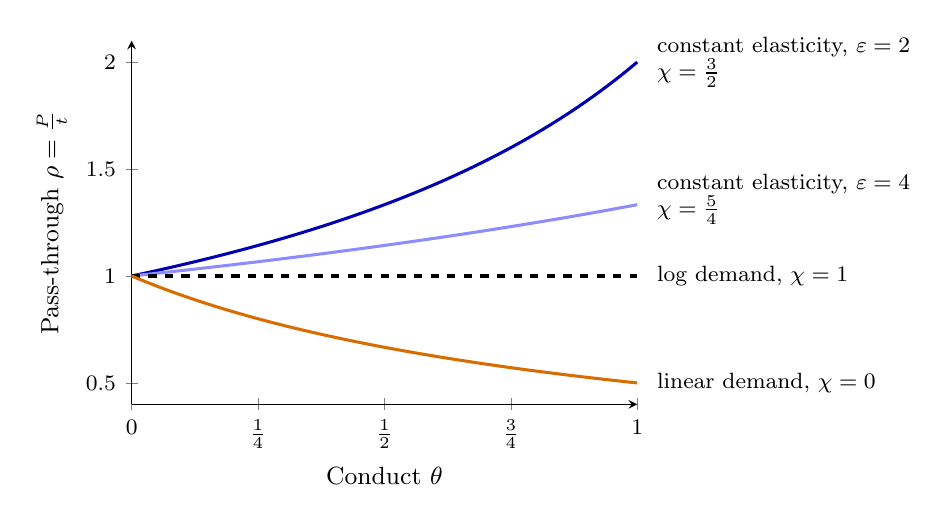
\begin{tikzpicture}
\begin{axis}[
  width=0.66\textwidth, height=6.2cm,
  xmin=0, xmax=1, ymin=0.4, ymax=2.1,
  xlabel={Conduct $\theta$}, ylabel={Pass-through $\rho = \frac{\dd P}{\dd t}$},
  xtick={0,0.25,0.5,0.75,1}, ytick={0.5,1,1.5,2},
  xticklabels={$0$,$\frac{1}{4}$,$\frac{1}{2}$,$\frac{3}{4}$,$1$},
  tick label style={font=\footnotesize}, label style={font=\small},
  axis lines=left, clip=false, every axis plot/.append style={line width=1.1pt}]
  \addplot[domain=0:1, samples=60, color=blue!70!black] {2/(2-x)};
  \addplot[domain=0:1, samples=60, color=blue!45] {4/(4-x)};
  \addplot[domain=0:1, samples=2, color=black, dashed] {1};
  \addplot[domain=0:1, samples=60, color=orange!85!black] {1/(1+x)};
  \node[anchor=west, font=\footnotesize, align=left] at (axis cs:1.02,2.0)
    {constant elasticity, $\varepsilon = 2$\\ $\chi = \frac{3}{2}$};
  \node[anchor=west, font=\footnotesize, align=left] at (axis cs:1.02,1.36)
    {constant elasticity, $\varepsilon = 4$\\ $\chi = \frac{5}{4}$};
  \node[anchor=west, font=\footnotesize, align=left] at (axis cs:1.02,1.0)
    {log demand, $\chi = 1$};
  \node[anchor=west, font=\footnotesize, align=left] at (axis cs:1.02,0.5)
    {linear demand, $\chi = 0$};
\end{axis}
\end{tikzpicture}
\caption{Pass-through of a specific tax as a function of conduct for four demand curves, with flat marginal cost. From
\cref{cor:03-passthrough-cases}, $\rho = \frac{1}{1 + \theta(1 - \chi)}$. Linear demand gives $\frac{1}{1 + \theta}$,
log demand gives 1 for every $\theta$, and constant elasticity gives $\frac{\varepsilon}{\varepsilon - \theta}$. The
dashed line is also the competitive benchmark.}
\label{fig:03-passthrough-curves}
\end{figure}

\begin{proposition}[What pass-through identifies]\label{prop:03-passthrough-id}
\Cref{cor:02-pt-reveal} gives the following. Under \cref{ass:03-passthrough} with flat marginal cost, pass-through
identifies only the composite
\begin{equation}\label{eq:03-kappa}
\kappa \equiv \theta(\chi - 1) = 1 - \frac{1}{\rho}.
\end{equation}
Consequently, the following hold.
\begin{enumerate}[label=(\roman*)]
\item $\rho > 1$ rejects $\theta = 0$ for every demand curve. Rising marginal cost only strengthens the rejection.
\item Any $\rho$ in $(0, \infty)$ is consistent with every conduct $\theta \in (0, 1]$, for a suitable curvature.
  Pass-through alone never rejects monopoly.
\item Under constant-elasticity demand with elasticity $\varepsilon$, $\theta = \varepsilon\kappa$.
\end{enumerate}
\end{proposition}

Equation \eqref{eq:03-kappa} is \eqref{eq:02-pt-kappa}. Part (i) combines parts (i) and (iii) of
\cref{cor:02-pt-reveal}. Parts (ii) and (iii) are parts (ii) and (iv) of that corollary. Given $\rho$ and conduct
$\theta > 0$, the curvature $\chi = 1 + \frac{\kappa}{\theta}$ reproduces the observed pass-through.

The proposition is the key to reading every cost pass-through study. A market-wide cost shock moves the equilibrium
along a single demand curve. What it reveals is the slope of perceived marginal revenue relative to the slope of demand,
and that slope mixes conduct with curvature. Separating them needs either an assumption on curvature, as in Sumner's
constant elasticity, or variation that changes the slope of demand at a given point (\cref{sec:03-identification}).

\subsection{Sumner's design and results}\label{sec:03-sumner-design}

\casehead{The question}
Is the US cigarette industry competitive, collusive, or in between? The industry was a textbook example of oligopoly.
In the Tobacco Case of 1946 the major manufacturers were convicted of operating an illegal cartel, and the consensus
was that their behavior did not change after the verdict \citep[p.~1010]{Sumner1981}. Earlier work had measured market
power by the ratio of price to marginal cost, which requires cost data that are rarely reliable. Sumner proposed a
scheme that avoids measuring cost: ``The coefficient of the tax rate term in a price equation identifies the ratio of
price to marginal cost'' \citep[p.~1010]{Sumner1981}.

\casehead{The setting}
Cigarettes carry a federal excise tax and state excise taxes, both specific taxes per pack. The federal tax was 8 cents
per pack for more than 25 years. The median state tax rose from 3 cents in 1954 to 12 cents in 1978. Combined taxes
nonetheless fell in real terms, from 48.7 percent of the retail price in 1954 to 35.5 percent in 1978. In 1978 state
taxes ranged from 2 cents in North Carolina to 21 cents in Florida, Connecticut and Massachusetts. The three states with
a large stake in tobacco growing and cigarette manufacturing (North Carolina, Virginia and Kentucky) all had low taxes.
Tobacco interests cannot explain the variation among the other states \citep[n.~8]{Sumner1981}.

Two features of the distribution system matter for the test. First, the institutions limit arbitrage across states.
The federal tax is paid by manufacturers, with the stamp affixed at the factory. Distributors must hold a license in the
state where they operate and must pay the state tax and affix its stamp within a few days of receiving a shipment.
Reselling out of state requires a special permit. Manufacturers therefore know the final state of sale and could, in
principle, set prices that depend on the state tax. Sumner argues that differentials of several cents per pack could
persist before arbitrage became profitable. Second, he assumes that wholesale and retail distribution are competitive,
citing the large numbers of retailers and distributors in each market.

\casehead{The data}
The panel covers 47 states and the District of Columbia annually from 1954 to 1978, 1,200 state-years. Alaska, Hawaii
and New Hampshire are excluded for lack of data and peculiar tax laws. Prices are the Tobacco Tax Council's
``weighted-average price per package'' for each state and year. The Council asks wholesalers for average retail prices
by type of cigarette (regular, king, 100 mm) and type of sale (carton, single pack, machine). It aggregates them with
national weights, so the most obvious quality differences are held fixed across states.

\casehead{The model}
Sumner starts from the markup rule of a firm $j$ facing a demand curve with elasticity $\eta_j < 0$ (his sign
convention),
\begin{equation*}
P_j = \frac{\eta_j}{\eta_j + 1}\, M_j \qquad \text{(his eq.~1)},
\end{equation*}
where $M_j$ is marginal cost. In our notation, with $\varepsilon_j = -\eta_j > 0$, this is
$P_j = \frac{\varepsilon_j}{\varepsilon_j - 1} M_j$. Under monopoly $\varepsilon_j$ is the market elasticity, and under
perfect competition it is infinite. Marginal cost is expanded as $M_j = X_j\beta + e_j + R$ (his eq.~2), with observed
cost factors $X_j$, unobserved factors $e_j$ and the tax $R$, which does not vary by firm.

Only state-average prices are observed, so Sumner aggregates. Let $S_j$ be firm $j$'s market share, $\omega_j \equiv
\frac{P_j}{M_j}$ its price-to-cost ratio, and $P = \sum_j S_j P_j$, $M = \sum_j S_j M_j$ and
$\bar\omega = \sum_j S_j\omega_j$ the share-weighted averages. Then
\begin{equation*}
P = \sum_j S_j\,\omega_j M_j = \bar\omega M + \sum_j S_j(\omega_j - \bar\omega)(M_j - M) \qquad \text{(his eq.~3)}.
\end{equation*}
To verify the identity, expand the last sum. It equals $\sum_j S_j\omega_j M_j - \bar\omega M - \bar\omega M +
\bar\omega M$, because $\sum_j S_j = 1$. Sumner also identifies $\bar\omega$ with $\frac{\bar\eta}{\bar\eta + 1}$ for
the share-weighted elasticity $\bar\eta$, which holds only approximately because the map is nonlinear. The covariance
term vanishes if price-cost ratios or marginal costs vary little across firms, or are unrelated. Sumner argues that
retail prices vary little across brands within a market and that costs are similar, since cigarettes are made in one
region with a standard technology. Dropping the covariance term gives $P = \bar\omega M$, and substituting the cost
equation gives the linear price equation
\begin{equation*}
P_{it} = X_{it}\psi + \bar\omega R_{it} + U_{it} \qquad \text{(his eq.~4)},
\end{equation*}
with states $i$, years $t$, $\psi = \bar\omega\beta$ and $U_{it} = \bar\omega e_{it}$. Sumner calls the tax coefficient
$\theta$. Under constant $\bar\omega$ it equals the pass-through $\frac{\dd P}{\dd R}$, so we write it as $\rho$.

The link to conduct is direct. With constant-elasticity market demand, flat marginal cost and conduct $\theta$,
\cref{cor:03-passthrough-cases}(iv) gives $P = \frac{\varepsilon}{\varepsilon - \theta}(k + t)$, with non-tax marginal
cost $k$ and tax $t$. Comparing with his eq.~1, Sumner's firm-level elasticity is
\begin{equation*}
\varepsilon_j = \frac{\varepsilon}{\theta},
\end{equation*}
the market elasticity divided by conduct. It is the elasticity that firms behave as if they face.

\casehead{The estimating equation and the estimator}
With states indexed by $s$ and years by $y$, the most complete specification is
\begin{equation}\label{eq:03-sumner-regression}
p_{sy} = \mu_s + \tau_y + \rho\, t_{sy} + e_{sy}.
\end{equation}
Here $p_{sy}$ is the price per pack and $t_{sy}$ the combined state and federal tax. The terms $\mu_s$ and $\tau_y$ are
state and year fixed effects. The state effects absorb $\frac{\varepsilon}{\varepsilon - \theta}k_{sy}$ to the extent that it is
constant within a state, and the year effects absorb national cost and price-level changes. Equation
\eqref{eq:03-sumner-regression} is a two-way fixed-effects, or difference-in-differences, regression
(\cref{app:econometrics}). Sumner estimates it by OLS. He also reports a specification that replaces the year effects
by the national consumer price index and drops the state effects. He estimates it by OLS and by a variance-components
(random-effects) generalized least squares (GLS) estimator with random state and year effects
\citep{FullerBattese1974}.

The hypotheses are sharp. Competition with flat marginal cost implies $\rho = 1$. Monopoly with constant-elasticity
demand implies $\rho = \frac{\varepsilon}{\varepsilon - 1} > 1$, and conduct $\theta$ implies
$\rho = \frac{\varepsilon}{\varepsilon - \theta}$. An estimate of $\rho$ can be inverted for the firm-level elasticity,
$\varepsilon_j = \frac{\rho}{\rho - 1}$.

\casehead{Identification}
Tax variation is treated as exogenous: the residual $e_{sy}$ is assumed uncorrelated with $t_{sy}$ given the fixed
effects. The state effects absorb stable differences in tax levels, such as the low taxes of producing states. What
identifies $\rho$ is therefore the timing of tax changes within states relative to other states. The assumption fails
if states raise taxes when local costs or demand change, or if taxes shift the demand for legal sales through
cross-border shopping and smuggling. The tax shifts the marginal cost of every seller in a state by the same amount, so
the test concerns market demand and industry conduct. A cost shifter specific to one firm would instead trace out that
firm's residual demand (\cref{sec:03-residual-demand}).

\casehead{Results}
\Cref{tab:03-sumner} reproduces Sumner's Table 1. With state and year effects, $\hat\rho = 1.074$ with a standard
error of 0.013. A 10-cent difference in taxes thus raises the price by 10.74 cents. The $t$-statistic for $\rho = 1$ is
$\frac{1.074 - 1}{0.013} = 5.7$. The other two specifications give 1.029 and 1.069, with $t$-statistics of 2.6 and 5.3.
All three reject competition at conventional levels. The last column of the table reports our replication on a
reconstructed panel (\cref{sec:03-sumner-replication}), which reproduces all three estimates to within 0.001.

\begin{table}[htbp]
\centering
\begin{threeparttable}
\caption{Effect of the excise tax on the retail price of cigarettes}
\label{tab:03-sumner}
\small
\begin{tabular}{@{}lccccccc@{}}
\toprule
& \multicolumn{4}{c}{Sumner (1981), Table 1} & \multicolumn{2}{c}{Implications} & Replication \\
\cmidrule(lr){2-5}\cmidrule(lr){6-7}\cmidrule(l){8-8}
& $\hat\rho$ & Elasticity & Controls & Method & $t$ for $\rho = 1$ & $\frac{\hat\rho}{\hat\rho - 1}$ &
  $\hat\rho$ \\
\midrule
(1) & \makecell{1.074\\(0.013)} & $-13.5$ & $DY_t$, $DS_i$ & OLS & 5.7 & 14.5 & \makecell{1.075\\(0.013)} \\
\addlinespace
(2) & \makecell{1.029\\(0.011)} & $-34.5$ & NCPI & OLS & 2.6 & 35.5 & \makecell{1.029\\(0.011)} \\
\addlinespace
(3) & \makecell{1.069\\(0.013)} & $-14.5$ & NCPI & VC & 5.3 & 15.5 & \makecell{1.069\\(0.013)} \\
\bottomrule
\end{tabular}
\begin{tablenotes}\footnotesize
\item Notes: The dependent variable is the retail price per pack in cents. The sample has 1,200 state-years (48 states
including DC, 1954--78). Standard errors are in parentheses. ``Elasticity'' is Sumner's implied price elasticity, with his negative sign.
$DY_t$ are year dummies (1978 excluded) and $DS_i$ state dummies (Wyoming excluded). NCPI is the national consumer
price index, and row (2) has no state dummies. VC is a variance-components (random-effects) GLS estimator with a random
effect for each state and each year. Sumner reports $R^2$ of about 0.99 with dummies and about 0.95 without. Our
replication gives 0.994 and 0.985. The column $\frac{\hat\rho}{\hat\rho - 1}$ inverts his eq.~1 exactly, in absolute
value. The replication uses OLS for rows (1) and (2) and two-way random-effects GLS for row (3), with conventional
standard errors, as in the paper.
\end{tablenotes}
\end{threeparttable}
\end{table}

The implied elasticities in the table deserve a check. Sumner's reported values equal $\frac{1}{1 - \hat\rho}$
exactly, for example $\frac{1}{1 - 1.074} = -13.5$. Inverting his eq.~1 exactly instead gives
$\eta_j = -\frac{\hat\rho}{\hat\rho - 1}$, which is $-14.5$, $-35.5$ and $-15.5$. The reported values thus treat
$\hat\rho - 1$ as the markup over cost, $\frac{P - M}{M} = -\frac{1}{\eta_j}$, in place of the Lerner condition
$\frac{P - M}{P} = -\frac{1}{\eta_j}$. The two agree to first order in $\frac{1}{\lvert\eta_j\rvert}$, so the
difference is immaterial for his conclusions. His text uses the same approximation: ``Taking $\theta = 1.05$, a 1
percent rise in the price of a firm's product would cause a 20 percent fall in the quantity sold'' \citep[p.~1019]{Sumner1981}.

\casehead{Robustness}
Sumner reports four checks. First, he estimates nonlinear versions of eq.~4 that let the price-to-cost ratio vary with
price, $\bar\omega(P) = \gamma P^{1 - \lambda}$. Substituting in $P = \bar\omega(P) M$ gives $P^{\lambda} = \gamma M$,
which he estimates by nonlinear least squares with additive and multiplicative errors (his eqs.~4$'$ and 4$''$). The
hypothesis $\lambda = 1$, under which the ratio is constant and equal to $\gamma$, is not rejected. The estimates are
$\hat\lambda = 0.972$ (0.027) and 0.981 (0.026), with $\hat\gamma = 1.029$ and 1.062 \citep[n.~9]{Sumner1981}.
Second, the pooled equation estimated separately for each year gives estimates in the range of Table 1, with no trend.
Third, a squared tax term added to the yearly equations is insignificant in most years. Smuggling would make price a
concave function of the tax, so this check speaks against a large role for smuggling. Fourth, adding New Hampshire
leaves the results essentially unchanged.

\casehead{Interpretation}
Sumner draws two conclusions. Pass-through significantly above one rejects atomistic competition. The implied
firm-level elasticities, between 13.5 and 34.5 in absolute value, are far above estimates of the industry elasticity
of demand, which ``are generally between $-0.3$ and $-0.8$'' \citep[p.~1017]{Sumner1981}. His own estimate of the
industry elasticity is about $-0.40$ (n.~10). A cartel acting as a monopolist would face the industry elasticity, so
the estimates are inconsistent with an effective cartel. A monopolist would never price on the inelastic part of
demand, so with an industry elasticity below one it would raise prices far above the observed level. Sumner concludes
that monopoly power is small relative to tax and other cost differences. Taking $\rho = 1.05$, it adds about 3 cents
to the average price of a pack.

In conduct-parameter language, the constant-elasticity model gives $\theta = \varepsilon\kappa$ with
$\kappa = 1 - \frac{1}{\rho}$ (\cref{prop:03-passthrough-id}). With $\hat\rho = 1.074$, $\hat\kappa = 0.069$. An
industry elasticity of 0.4 then gives $\theta \approx 0.028$, and the range from 0.3 to 0.8 gives $\theta$ between 0.021
and 0.055. These values are close to competition. They correspond to the conduct of a symmetric Cournot industry with
18 to 48 firms, in an industry with only six major manufacturers \citep[p.~488]{AshenfelterSullivan1987}.
Sumner's alternative explanation is Barzel's (\citeyear{Barzel1976}) quality effect, which we discuss with the other
critiques below.

\subsection{Curvature, cost, composition, and further critiques}\label{sec:03-sumner-critiques}

Sumner's rejection of competition needs only flat marginal cost. His rejection of collusion also needs
constant-elasticity demand. Three critiques address these assumptions and the price measure.

\casehead{Demand curvature}
\Cref{prop:03-passthrough-id} shows that a pass-through test identifies conduct only conditional on curvature. A
monopolist facing log demand passes through exactly one, the competitive value
(\cref{cor:03-passthrough-cases}(vi)). A monopolist facing concave or linear inverse demand passes through less than
one. A pass-through below one would then wrongly ``accept'' competition, or even suggest that firms absorb taxes.
Sumner's nonlinear check tests whether pass-through varies with the price level. Constant pass-through is consistent
with constant elasticity, but also with any other pair $(\theta, \chi)$ whose product $\theta(\chi - 1)$ stays constant.
It cannot pin down curvature on its own.

\casehead{Cost curvature}
With rising marginal cost, competitive pass-through is $\frac{\varepsilon_S}{\varepsilon_S + \varepsilon} < 1$
(\cref{cor:03-passthrough-cases}(i)). A pass-through near one is then consistent with several combinations:
competition with flat marginal cost, monopoly with log demand, or monopoly with log-convex demand and rising marginal
cost. The slope of marginal cost and conduct both enter the slope of the supply relation. This is the identification
problem of \cref{sec:03-identification} in another guise. Rising marginal cost pushes competitive pass-through below
one, so it leaves the rejection of competition intact.

\casehead{Composition}
Sumner's price is an average over brands and package types. Suppose the measured price is $\bar p = \sum_j w_j p_j$,
with quantity weights $w_j$. Then
\begin{equation*}
\frac{\dd \bar p}{\dd t} = \sum_j w_j\,\frac{\dd p_j}{\dd t} + \sum_j p_j\,\frac{\dd w_j}{\dd t}.
\end{equation*}
The first term is the average pass-through of individual prices. The second is a composition effect. A specific tax
raises the prices of cheap varieties proportionally more than those of expensive ones, so consumers may trade up. The
second term is then positive, and the regression overstates product-level pass-through. The test is biased toward
rejecting competition. The Tobacco Tax Council's fixed national weights remove composition effects across package types
and types of sale, but not across brands within a type. Sumner's observation that retail prices vary little across brands limits this
channel. \citet[p.~13]{NevoHatzitaskos2005} make a related point in another
setting. Much of the fall in the average price of tuna during Lent, a period of high demand, comes from a shift of
purchases toward cheaper products.

A close relative of the composition effect is the quality response emphasized by \citet{Barzel1976}. A per-unit tax
lowers the relative price of quality, so higher taxes should induce higher quality per unit. Measured price per pack
then rises by more than the tax even under competition. Sumner replies that the price data hold the obvious quality
dimensions fixed and that centralized manufacturing leaves little room for quality variation across states. He also
notes that a Barzel effect would bias the estimate upward, which strengthens the case against an effective cartel
\citep[p.~1018]{Sumner1981}.

\casehead{Further critiques}
Four further issues apply to any tax pass-through study. First, taxes shift demand as well as cost. Consumers in
high-tax states buy across borders or from smugglers, so legal sales respond to the tax beyond the movement along
demand. Sumner's own footnote 6 notes that smuggling can lower measured prices net of tax at both extremes. In very
low-tax states, bulk sales for export carry low transaction costs. In very high-tax states, legal sellers compete with
the illegal market. Second, timing matters. Prices are observed once a year, and announced tax increases can trigger
stockpiling and anticipatory price changes, so annual data may mix short-run and long-run pass-through. Third, the
test measures the conduct of the whole vertical chain. Market power among wholesalers or retailers, or retailers who
apply percentage markups, would also produce $\rho > 1$ with competitive manufacturers. Fourth, the regression errors
are serially correlated within states, so conventional standard errors overstate precision
\citep{BertrandDufloMullainathan2004}. \Cref{sec:03-sumner-replication} shows that clustering by state matters here.
Specific and ad valorem taxes also pass through differently. An ad valorem tax at rate $\tau$ on the consumer price
scales effective marginal cost by $\frac{1}{1 - \tau}$. Its pass-through therefore depends on the level of cost as well
as on curvature.

\subsection{A replication and what it adds}\label{sec:03-sumner-replication}

We re-estimate Sumner's regressions on a reconstructed panel with the same coverage: 47 states and the District of
Columbia, 1954 to 1978, 1,200 state-years. Prices and taxes come from \citet[Table~13]{TobaccoInstitute1983}, the historical
compilation of \emph{The Tax Burden on Tobacco}. They are nominal cents per pack on November 1 of each year. The tax is the state tax plus the
federal tax of 8 cents, and municipal taxes are excluded. We deflate by the consumer price index for all urban consumers (CPI-U) where needed. The average price rises
from 22.5 cents in 1954 to 56.6 cents in 1978. The median state tax rises from 3 to 12 cents, as in Sumner's
footnote 8. The same footnote gives a stronger check. In the reconstructed panel the median combined tax is 48.7
percent of the median price in 1954 and 35.3 percent in 1978, against Sumner's 48.7 and 35.5 percent. Of the 1,152 year-to-year transitions within states, 191 involve a tax change. Only 6 are
decreases, and the average change is 2.4 cents. The tax accounts for 46.7 percent of the retail price on average.

\Cref{tab:03-sumner} shows that the reconstructed data reproduce all three of Sumner's estimates. \Cref{tab:03-replication}
reports three extensions, and \cref{app:problems} develops the exercise in full.

\begin{table}[htbp]
\centering
\begin{threeparttable}
\caption{Replication and extensions of the pass-through regression}
\label{tab:03-replication}
\small
\setlength{\tabcolsep}{5pt}
\begin{tabular}{@{}llcc@{}}
\toprule
Specification & Statistic & Estimate & S.e. \\
\midrule
M0: nominal cents, state and year effects & $\hat\rho$ & 1.075 & 0.013 \\
  & $\hat\rho$, state-clustered s.e. & 1.075 & 0.034 \\
  & 95\% confidence interval & \multicolumn{2}{c}{$[1.006,\ 1.143]$} \\
  & $p$-value for $\rho = 1$ (clustered) & \multicolumn{2}{c}{0.033} \\
\addlinespace
M1: real cents, state and year effects & $\hat\rho$ & 1.107 & 0.026 \\
\addlinespace
M2: quadratic in the real tax & $\hat\rho$ at 10th percentile of tax & 1.097 & 0.039 \\
  & $\hat\rho$ at 90th percentile of tax & 1.113 & 0.034 \\
  & $p$-value for $b_2 = 0$ & \multicolumn{2}{c}{0.76} \\
  & 95\% interval for $\rho(p_{90}) - \rho(p_{10})$ & \multicolumn{2}{c}{$[-0.090,\ 0.122]$} \\
\addlinespace
Composite from M0 & $\hat\kappa = 1 - \frac{1}{\hat\rho}$ & 0.069 & \\
  & 95\% interval for $\kappa$ & \multicolumn{2}{c}{$[0.006,\ 0.125]$} \\
\bottomrule
\end{tabular}
\begin{tablenotes}\footnotesize
\item Notes: 1,200 state-years. All specifications include state and year fixed effects. Standard errors are clustered
by state (48 clusters) except in the first row. M1 deflates price and tax by the CPI-U. M2 regresses the real price
on $b_1(T_{sy} - \bar T) + b_2(T_{sy} - \bar T)^2$, so that $\rho(T) = b_1 + 2b_2(T - \bar T)$. The interval for
$\kappa$ maps the endpoints of the clustered interval for $\rho$. $\hat\kappa$ uses the unrounded estimate
$\hat\rho = 1.0746$.
\end{tablenotes}
\end{threeparttable}
\end{table}

\casehead{Clustering}
Sumner's conventional standard error of 0.013 ignores serial correlation of the errors within states. Clustering by
state raises it to 0.034. Pass-through remains significantly above one, with a 95 percent interval of $[1.006, 1.143]$
and $p = 0.033$. The rejection of competition survives, but its margin is much thinner than a $t$-statistic of 5.7
suggests. In real terms (M1) the estimate is 1.107 with a clustered standard error of 0.026.

\casehead{Constant pass-through}
If conduct and curvature are constant, pass-through does not vary with the tax. Specification M2 lets it vary
through a quadratic in the real tax. Estimated pass-through is 1.097 at the 10th percentile of the tax and 1.113 at
the 90th, and the test of $b_2 = 0$ gives $p = 0.76$. The test has little power, however. The 95 percent interval for
the difference between the two percentiles is wider than $\hat\rho - 1$ itself.

\casehead{The identified set}
By \cref{prop:03-passthrough-id}, the data identify $\hat\kappa = 0.069$, with 95 percent interval
$[0.006, 0.125]$. Every pair $(\chi, \theta)$ on the hyperbola $\theta(\chi - 1) = \hat\kappa$ fits the estimate
equally well. \Cref{fig:03-identified-set} plots this set. Monopoly fits with $\chi = 1.069$, a demand curve slightly
more convex than log demand. Symmetric Cournot with six firms fits with $\chi = 1.42$. Constant elasticity with an
industry elasticity of 0.4 has $\chi = 3.5$ and gives $\theta = 0.028$, with interval $[0.002, 0.050]$. The data alone
cannot choose among these. Sumner's rejection of collusion rests on the constant-elasticity assumption combined with
outside estimates of the industry elasticity.

\begin{figure}[htbp]
\centering
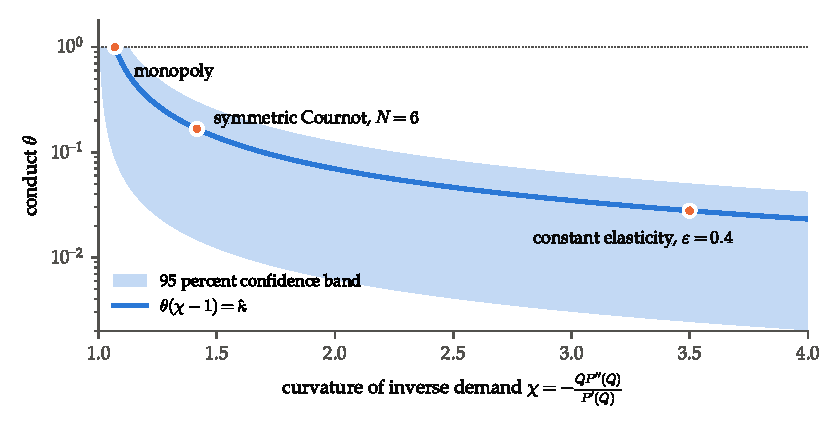
\includegraphics[width=0.9\textwidth]{figures/ch03/sumner_identified_set.pdf}
\caption{Pairs of demand curvature $\chi$ and conduct $\theta$ consistent with the estimated cigarette tax pass-through
$\hat\rho = 1.0746$. The curve is $\theta(\chi - 1) = \hat\kappa$ with $\hat\kappa = 0.069$, and the band maps the 95
percent state-clustered confidence interval for $\rho$. The marked points are monopoly ($\chi = 1.069$), symmetric
Cournot with six firms ($\chi = 1.42$, $\theta = \frac{1}{6}$) and constant-elasticity demand with $\varepsilon = 0.4$
($\chi = 3.5$, $\theta = 0.028$). The vertical axis is logarithmic.}
\label{fig:03-identified-set}
\end{figure}

\casehead{A bound that does not depend on curvature}
Outside information on the industry elasticity can rule out monopoly without any assumption on curvature. With flat
marginal cost $c \ge 0$ and tax $t$, the Lerner form of \eqref{eq:03-supply-tax} is
$\frac{P - t - c}{P} = \frac{\theta}{\varepsilon}$, where $\varepsilon$ is the elasticity at the observed equilibrium.
Since $c \ge 0$,
\begin{equation}\label{eq:03-lerner-bound}
\theta = \varepsilon\Bigl(1 - \frac{t}{P} - \frac{c}{P}\Bigr) \le \varepsilon\Bigl(1 - \frac{t}{P}\Bigr).
\end{equation}
The tax is a large share of the cigarette price. At the sample mean share of 0.467 and $\varepsilon = 0.4$, the bound
gives $\theta \le 0.213$. At the lowest share in the sample (0.229) it gives $\theta \le 0.308$. Both rule out monopoly.
Equivalently, monopoly at the mean tax share requires an elasticity of at least $\frac{1}{1 - 0.467} = 1.88$ at the
observed price. The bound uses the level of prices and taxes, and pass-through does not enter it. Sullivan's bound in
\cref{sec:03-sullivan} develops the same idea with an elasticity estimated from the tax variation itself.

\begin{remark}[Pass-through as a tool]\label{rem:03-passthrough-tool}
\Cref{prop:03-passthrough} turns pass-through into a measurement device. Given estimates of $\rho$, $\varepsilon$
and the slope of marginal cost, it pins down conduct for any assumed curvature. Conversely, given conduct, it predicts
the incidence of taxes and cost shocks. \citet{WeylFabinger2013} develop this program in general. Recent applications
combine first-order conditions of this kind with credible sources of variation. \citet{MillerOsborneSheu2017} study
the US portland cement industry from 1980 to 2010. Their estimated pass-through of fuel costs ranges from 1.03 to 1.65
across specifications (Table~4, p.~84). They combine it with conduct estimates from earlier work to measure the incidence
of a price on carbon emissions.
\citet{BergquistDinerstein2020} use the first-order-condition approach to estimate the effect of coordination among
intermediaries in the Kenyan maize market. Their field experiment supplies the instruments
\citep[p.~214, n.~86]{AskerNocke2021}.
Identification of conduct still requires curvature, which must come from demand estimated over a range of prices or
from assumption.
\end{remark}

\casehead{Contribution}
Sumner's paper introduced a design that is now standard. It uses an observed, exogenous component of marginal cost
and a fixed-effects panel to learn about the pricing rule without measuring cost. Its rejection of competition holds for
any demand curve and any non-decreasing marginal cost, although clustering weakens it. Its rejection of collusion holds
only given curvature, or given an industry elasticity and the curvature-free bound \eqref{eq:03-lerner-bound}. The
lesson extends beyond cigarettes. A market-wide cost shifter traces out demand and reveals the slope of perceived
marginal revenue, which mixes conduct with curvature. Cost shifters therefore deliver tests and bounds on conduct.
Point identification requires variation that rotates demand (\cref{sec:03-identification}), cost shifters specific to
one firm (\cref{sec:03-residual-demand}), or direct measures of cost (\cref{sec:03-sugar,sec:03-electricity}).

\section{Comparative statics in cost without functional forms}\label{sec:03-revenue-tests}

Sumner's test in \cref{sec:03-sumner} turns a cost shock into a statement about conduct. It does so by
assuming a demand curve with constant elasticity and a flat marginal cost. This section studies three tests
that drop those functional forms. Each test asks what profit maximization alone implies about the response
of an equilibrium to a change in cost. The answers are inequalities. They can reject monopoly or bound
conduct from above, but they rarely deliver a point estimate.

We proceed in three steps. We first derive the bound of \citet{Sullivan1985} and explain why cost shifters
can only produce inequalities. We then prove the revealed-preference test of \citet{AshenfelterSullivan1987}
and report its evidence from the cigarette industry. Finally we develop the revenue test of
\citet{PanzarRosse1987}, which needs data on revenue and factor prices only.

\subsection{Sullivan's bound and why cost shifters give only inequalities}\label{sec:03-sullivan}

Consider $N$ firms selling a homogeneous good. Inverse demand $P(Q)$ is stable and decreasing, $P' < 0$.
Firm $i$ has cost $C_i(q_i) + t q_i$, where $t$ is a specific tax paid by sellers and $C_i$ is increasing.
Its marginal cost is therefore $MC_i = C_i'(q_i) + t \ge t$. Following \citet[eq.~24]{Bresnahan1989}, we
write the first-order condition of firm $i$ in conjectural-variations form,
\begin{equation}\label{eq:03-cv-foc}
  P(Q) + (1 + r_i)\, q_i P'(Q) = MC_i, \qquad i = 1, \dots, N,
\end{equation}
where $r_i$ is the conjectural variation $\frac{\dd Q_{-i}}{\dd q_i}$ of \cref{sec:03-objects}. Cournot behavior is
$r_i = 0$, joint profit maximization by $N$ identical firms is $1 + r_i = N$, and price taking is the limit
$1 + r_i \to 0$. As in \cref{sec:03-objects}, $r_i$ describes how close output is to the competitive and
collusive levels. It makes no claim about what firms believe.

\begin{definition}[Numbers equivalent]\label{def:03-numbers-equivalent}
Suppose $1 + r_i > 0$ for every $i$. The \emph{numbers equivalent} of the industry is
\begin{equation*}
  N_e = \sum_{i=1}^{N} \frac{1}{1 + r_i}.
\end{equation*}
\end{definition}

In a Cournot industry $N_e = N$, so $N_e$ counts the Cournot firms that would produce the same conduct. A
cartel of $N$ identical firms has $N_e = N \cdot \frac{1}{N} = 1$, and price taking corresponds to $N_e \to
\infty$. The next lemma connects $N_e$ to the industry conduct parameter of \eqref{eq:03-supply-relation}.

\begin{lemma}\label{lem:03-cv-aggregation}
If all firms have the same marginal cost $c$, the conditions \eqref{eq:03-cv-foc} aggregate to the supply
relation $P + \theta Q P'(Q) = c$ with $\theta = \frac{1}{N_e}$.
\end{lemma}

\begin{proof}
Rearrange \eqref{eq:03-cv-foc} as $P - c = -(1 + r_i) q_i P'$ and divide by $1 + r_i$:
\begin{equation*}
  \frac{P - c}{1 + r_i} = -q_i P'.
\end{equation*}
Summing over $i$ gives $(P - c) N_e = -Q P'$. Dividing by $N_e$ gives $P + \frac{1}{N_e} Q P' = c$.
\end{proof}

The lemma is a special case of \cref{prop:03-aggregation}. With a common marginal cost, each firm's condition reads
$s_i(1 + r_i) = \varepsilon\frac{P - c}{P}$, so every firm has the same value of $s_i\tilde\theta_i$. The industry
conduct $\sum_i \varphi_i s_i \tilde\theta_i$ is then the same for all weights, and the lemma shows that it equals
$\frac{1}{N_e}$.

Now let $z_c > 0$ be any variable that shifts marginal cost and is excluded from demand. The tax is the
leading example, and a factor price is another. Write the equilibrium price and output as $P^*(z_c)$ and
$Q^*(z_c)$. The \emph{reduced-form elasticities} of price and quantity with respect to the cost shifter are
\begin{equation}\label{eq:03-EP-EQ}
  E_P = \frac{\dd \ln P^*}{\dd \ln z_c}, \qquad E_Q = \frac{\dd \ln Q^*}{\dd \ln z_c}.
\end{equation}
\citet{Bresnahan1989} writes them $H_P$ and $H_Q$. Both can be estimated from regressions of log price and log
output on the cost shifter. The first result says what they reveal.

\begin{lemma}[Cost shifters trace out demand]\label{lem:03-trace-demand}
If $z_c$ does not enter demand and $E_P \neq 0$, the demand elasticity at the observed equilibrium is
$\varepsilon = -\frac{E_Q}{E_P}$, whatever the conduct, the slope of marginal cost and the curvature of
demand.
\end{lemma}

\begin{proof}
Every equilibrium lies on the same demand curve, so $P^*(z_c) = P(Q^*(z_c))$ for all $z_c$. Differentiating
in $z_c$ gives $\frac{\dd P^*}{\dd z_c} = P'(Q^*)\frac{\dd Q^*}{\dd z_c}$. Multiply both sides by
$\frac{z_c}{P^*}$ and insert $\frac{Q^*}{Q^*}$:
\begin{equation*}
  E_P = \frac{Q^* P'(Q^*)}{P^*} \cdot \frac{z_c}{Q^*}\frac{\dd Q^*}{\dd z_c} = -\frac{1}{\varepsilon}\, E_Q .
\end{equation*}
Solving for $\varepsilon$ completes the proof.
\end{proof}

\begin{proposition}[Sullivan's bound]\label{prop:03-sullivan-bound}
Suppose $1 + r_i > 0$ and $MC_i \ge t$ for every firm, and let $z_c$ satisfy \cref{lem:03-trace-demand}. Then
\begin{equation}\label{eq:03-sullivan-bound}
  N_e \;\ge\; \frac{1}{\varepsilon\left(1 - \frac{t}{P}\right)} \;=\; -\frac{E_P}{E_Q}\cdot\frac{P}{P - t}.
\end{equation}
If, in addition, all firms share the marginal cost $c$, conduct satisfies
\begin{equation}\label{eq:03-sullivan-theta}
  \theta = \varepsilon L = -L\,\frac{E_Q}{E_P} \;\le\; -\frac{E_Q}{E_P}\left(1 - \frac{t}{P}\right).
\end{equation}
\end{proposition}

\begin{proof}
By \eqref{eq:03-cv-foc}, $P - MC_i = -(1 + r_i) q_i P' > 0$, so $P > MC_i \ge t$. Divide by $1 + r_i > 0$ and
use $MC_i \ge t$:
\begin{equation*}
  \frac{P - t}{1 + r_i} \;\ge\; \frac{P - MC_i}{1 + r_i} \;=\; -q_i P'.
\end{equation*}
Sum over $i$ and use $-QP' = \frac{P}{\varepsilon}$:
\begin{equation*}
  (P - t)\, N_e \;\ge\; -Q P' \;=\; \frac{P}{\varepsilon}.
\end{equation*}
Divide by $P - t > 0$ to get $N_e \ge \frac{P}{\varepsilon (P - t)}$, which is the first expression in
\eqref{eq:03-sullivan-bound}. Substituting $\varepsilon = -\frac{E_Q}{E_P}$ from \cref{lem:03-trace-demand}
gives the second. Under a common marginal cost, \cref{lem:03-cv-aggregation} gives $\theta = \frac{1}{N_e}$
and \eqref{eq:03-lerner-theta} gives $\theta = \varepsilon L$. Finally $c \ge t$ implies $L \le 1 -
\frac{t}{P}$.
\end{proof}

Three features of the bound matter for what follows. First, it uses two reduced-form elasticities and the
tax share of the price. Nothing depends on the curvature of demand, the slope of marginal cost or the
functional form of either. Second, it is one-sided. A large value of the right side of
\eqref{eq:03-sullivan-bound} rejects collusive conduct, but no value can reject competition, because $N_e =
\infty$ satisfies every lower bound. Third, it is the Lerner bound \eqref{eq:03-lerner-bound} of
\cref{sec:03-sumner-replication} with the demand elasticity estimated from the cost shock itself.

\citet[eq.~25]{Bresnahan1989} states the bound in the form
\begin{equation*}
  \sum_i (1 + r_i)^{-1} \;\ge\; -\frac{H_P}{H_Q L} \;\ge\; -\frac{H_P}{H_Q},
\end{equation*}
with $H_P$ and $H_Q$ our $E_P$ and $E_Q$ and $L$ the common Lerner index. The first relation holds with
equality under a common marginal cost, by \cref{lem:03-cv-aggregation}. The second uses only $L \le 1$, that
is $MC \ge 0$, and coincides with \eqref{eq:03-sullivan-bound} at $t = 0$. Using the tax as a floor on
marginal cost tightens the bound, and this is the refinement that Sullivan uses
\citep[p.~1038]{Bresnahan1989}. For a cartel ($N_e = 1$) the bound says that $\varepsilon(1 - \frac{t}{P})
\ge 1$. A monopolist never prices on the inelastic part of demand, and the tax sharpens that rule. Its Lerner
index $\frac{1}{\varepsilon}$ cannot exceed the share of the price left after tax.

\begin{example}[An illustrative calculation]\label{ex:03-sullivan}
Suppose a 10 percent tax increase raises the price by 4 percent and lowers sales by 1.6 percent. Suppose
also that the tax is 40 percent of the price. These numbers are illustrative only. Then $E_P = 0.4$, $E_Q =
-0.16$ and $\varepsilon = \frac{0.16}{0.4} = 0.4$. The bound is
\begin{equation*}
  N_e \;\ge\; \frac{1}{0.4 \times (1 - 0.4)} = \frac{1}{0.24} \approx 4.2,
  \qquad \theta \;\le\; 0.24 .
\end{equation*}
Monopoly and Cournot conduct with up to four firms are rejected. Cournot conduct with five or more firms
is not.
\end{example}

\citet{Sullivan1985} applies the bound to a panel of U.S. states and years in the cigarette industry. State
excise taxes are the cost shifter, and an analysis-of-variance procedure absorbs the other exogenous
variables. He rejects the hypothesis that cigarette prices are set as if by a cartel
\citep[p.~1038]{Bresnahan1989}. \citet[p.~496]{AshenfelterSullivan1987} summarize his finding as industry
behavior inconsistent with a numbers equivalent below two or three.

\casehead{Why cost shifters give only inequalities} The proof of \cref{lem:03-trace-demand} shows what a
cost shifter does. Demand does not move, so every observed equilibrium lies on one demand curve, and
variation in $z_c$ traces that curve out. A cost shifter therefore identifies the demand elasticity at each
observed point. Conduct, however, sits in the supply relation, which in Lerner form reads $P - MC =
\theta\frac{P}{\varepsilon}$. Once $\varepsilon$ is known, $\theta$ is pinned down only if the level of
marginal cost is known. The data restrict it only to $t \le MC \le P$. Mapping these two bounds through the
supply relation gives the identified set
\begin{equation}\label{eq:03-cost-identified-set}
  0 \;\le\; \theta \;\le\; \varepsilon\left(1 - \frac{t}{P}\right).
\end{equation}
A demand shifter works the other way round. It moves equilibria along the supply relation and so traces out
the equation that contains $\theta$. \citet[p.~1039]{Bresnahan1989} draws this contrast, and
\cref{sec:03-identification} shows when demand shifters identify conduct. Pass-through is a partial
exception. The slope of price in cost does involve $\theta$, but \cref{prop:03-passthrough-id} shows that it
confounds conduct with the curvature of demand and the slope of marginal cost.

\subsection{Ashenfelter and Sullivan (1987): a revealed-preference test}\label{sec:03-ashenfelter-sullivan}

\casehead{Question} Parametric tests of monopoly fit equations of a chosen functional form and then test
restrictions on them. \citet{AshenfelterSullivan1987} point out that such a procedure always tests a joint
hypothesis. They quote \citet[p.~99]{Varian1983}: such a procedure tests ``whatever one wants to test plus
the maintained hypothesis of functional form.'' They therefore adapt the nonparametric
revealed-preference approach of \citet{Afriat1967} and \citet{Varian1982} to monopoly. Excise taxes are
well suited to it. Large tax changes give the test power, and every tax change yields a separate prediction.
The researcher can therefore report the percentage of correct predictions, which separates a model that
fails as a rule from one that fails occasionally (p.~484).

\casehead{The test} An industry acts as a single decision maker, a monopoly or a perfect cartel. It faces a
decreasing inverse demand $P(q)$ and a cost $C(q) = C_0(q) + tq$, where $C_0$ is increasing and $t$ is the
excise tax per unit. Let $t_0 < t_1$ be two tax rates with the same $P$ and $C_0$. Let $q_0$ and $q_1$ be the
profit-maximizing outputs and $p_0 = P(q_0)$, $p_1 = P(q_1)$ the prices.

\begin{proposition}[Ashenfelter and Sullivan]\label{prop:03-as-inequality}
Under these assumptions:
\begin{enumerate}[label=(\roman*)]
  \item Output does not rise and price does not fall, $q_1 \le q_0$ and $p_1 \ge p_0$.
  \item Revenue falls by at least the old tax times the fall in output,
  \begin{equation}\label{eq:03-as-revenue}
    p_1 q_1 - p_0 q_0 \;\le\; t_0\,(q_1 - q_0).
  \end{equation}
  \item If $p_1 > p_0$, the arc elasticity of demand satisfies
  \begin{equation}\label{eq:03-as-arc}
    \frac{(q_0 - q_1)\, p_0}{(p_1 - p_0)\, q_0} \;\ge\; \frac{p_0}{p_1 - t_0}.
  \end{equation}
\end{enumerate}
\end{proposition}

\begin{proof}
Output $q_0$ is optimal at tax $t_0$, so it earns at least as much as $q_1$ would:
\begin{equation}\label{eq:03-as-rp0}
  p_0 q_0 - C_0(q_0) - t_0 q_0 \;\ge\; p_1 q_1 - C_0(q_1) - t_0 q_1 .
\end{equation}
Output $q_1$ is optimal at tax $t_1$:
\begin{equation}\label{eq:03-as-rp1}
  p_1 q_1 - C_0(q_1) - t_1 q_1 \;\ge\; p_0 q_0 - C_0(q_0) - t_1 q_0 .
\end{equation}
Add the two inequalities. Revenues and the $C_0$ terms cancel, which leaves
\begin{equation*}
  -t_0 q_0 - t_1 q_1 \;\ge\; -t_0 q_1 - t_1 q_0
  \quad\Longleftrightarrow\quad
  (t_1 - t_0)(q_0 - q_1) \;\ge\; 0 .
\end{equation*}
Since $t_1 > t_0$, $q_1 \le q_0$. Demand slopes down, so $p_1 \ge p_0$. This proves (i). Rearrange
\eqref{eq:03-as-rp0}:
\begin{equation*}
  p_1 q_1 - p_0 q_0 \;\le\; \bigl[C_0(q_1) - C_0(q_0)\bigr] + t_0 (q_1 - q_0).
\end{equation*}
The bracket is not positive because $q_1 \le q_0$ and $C_0$ is increasing. This proves (ii). For (iii),
write $p_1 q_1 - p_0 q_0 = p_1(q_1 - q_0) + q_0(p_1 - p_0)$ and substitute into \eqref{eq:03-as-revenue}:
\begin{equation*}
  q_0 (p_1 - p_0) \;\le\; (p_1 - t_0)(q_0 - q_1).
\end{equation*}
A monopolist prices above marginal cost, so $p_1 > t_1 > t_0$. Multiply both sides by the positive number
$\frac{p_0}{q_0 (p_1 - p_0)(p_1 - t_0)}$ to obtain \eqref{eq:03-as-arc}.
\end{proof}

Inequality \eqref{eq:03-as-revenue} has a direct reading. Moving from $q_0$ to $q_1$ saves $t_0(q_0 - q_1)$
in taxes at the old rate. The revenue lost by the move must exceed this saving. Otherwise the monopolist
would have chosen $q_1$ when the tax was still $t_0$. Inequality \eqref{eq:03-as-arc} extends the rule that a
monopolist never produces on the inelastic part of demand. The arc elasticity must exceed
$\frac{p_0}{p_1 - t_0}$, which is above one whenever the price rises by less than the old tax. The test uses
two observed points, no functional form, no derivatives and no convexity of cost. It is local because it
compares points close in time, where demand and cost are plausibly the same. \Cref{fig:03-as-test} draws the
logic in the plane of output and revenue.

\begin{figure}[htbp]
\centering
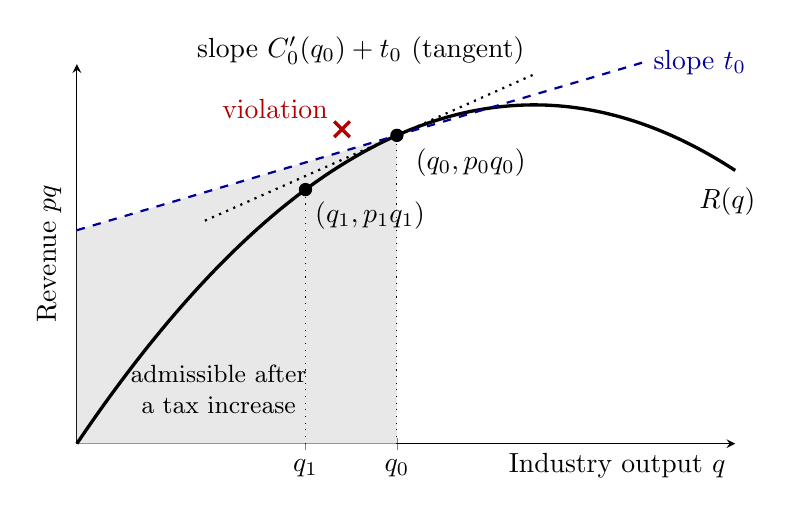
\begin{tikzpicture}
\begin{axis}[
  width=0.82\textwidth, height=6.4cm,
  xmin=0, xmax=7.2, ymin=0, ymax=28,
  axis lines=left,
  xlabel={Industry output $q$}, ylabel={Revenue $pq$},
  xtick={2.5,3.5}, xticklabels={$q_1$,$q_0$},
  ytick=\empty, clip=false,
  every axis x label/.style={at={(ticklabel* cs:1.0)}, anchor=north east}
]
  \addplot[fill=gray!18, draw=none] coordinates {(0,0) (0,15.75) (3.5,22.75) (3.5,0)} -- cycle;
  \addplot[domain=0:7.2, samples=120, very thick, black] {10*x - x^2};
  \node[anchor=north west] at (axis cs:6.7,19.6) {$R(q)$};
  \addplot[domain=0:6.2, thick, dashed, blue!60!black] {22.75 + 2*(x - 3.5)};
  \node[anchor=west, blue!60!black] at (axis cs:6.2,28.15) {slope $t_0$};
  \addplot[domain=1.4:5.0, thick, dotted, black] {22.75 + 3*(x - 3.5)};
  \node[anchor=south east] at (axis cs:5.0,27.25) {slope $C_0'(q_0) + t_0$ (tangent)};
  \addplot[only marks, mark=*, mark size=2.2pt] coordinates {(3.5,22.75) (2.5,18.75)};
  \node[anchor=north west] at (axis cs:3.6,22.5) {$(q_0, p_0 q_0)$};
  \node[anchor=north west] at (axis cs:2.5,18.6) {$(q_1, p_1 q_1)$};
  \addplot[only marks, mark=x, mark size=4pt, very thick, red!70!black] coordinates {(2.9,23.2)};
  \node[anchor=south east, red!70!black] at (axis cs:2.85,23.3) {violation};
  \draw[dotted] (axis cs:3.5,0) -- (axis cs:3.5,22.75);
  \draw[dotted] (axis cs:2.5,0) -- (axis cs:2.5,18.75);
  \node[anchor=center, align=center, font=\small] at (axis cs:1.55,4.0) {admissible after\\ a tax increase};
\end{axis}
\end{tikzpicture}
\caption{The revealed-preference logic of \cref{prop:03-as-inequality}. After the tax rises from $t_0$ to
$t_1$, the new point $(q_1, p_1q_1)$ must lie left of $q_0$ and below the line through $(q_0, p_0q_0)$ with
slope $t_0$ (shaded region). The tangent of the revenue curve at $q_0$ has slope equal to marginal revenue,
$C_0'(q_0) + t_0$, which is at least $t_0$. A point above the dashed line, such as the cross, rejects monopoly
with stable demand and cost. The curve is drawn for $R(q) = 10q - q^2$, $C_0' = 1$, $t_0 = 2$ and $t_1 =
4$.}
\label{fig:03-as-test}
\end{figure}

\casehead{A conduct index} The test extends to intermediate conduct. Following
\citet[eq.~12]{AshenfelterSullivan1987}, who call the index $\beta$, say that the industry has
\emph{conduct index} $\theta \in [0, 1]$ if, at its chosen output $q$,
\begin{equation}\label{eq:03-as-index}
  \Delta q\, P(q + \Delta q) + \theta\, q \bigl[P(q + \Delta q) - P(q)\bigr] \;\le\; C(q + \Delta q) - C(q)
  \quad \text{for all } \Delta q .
\end{equation}
With $\theta = 1$ the left side equals $(q + \Delta q)P(q + \Delta q) - qP(q)$, so \eqref{eq:03-as-index} is the
monopoly optimality condition. With $\theta = 0$ it is the revealed-preference form of price equal to marginal
cost. Dividing \eqref{eq:03-as-index} by $\Delta q > 0$ and letting $\Delta q \to 0$ gives $P + \theta q P'
\le C'$. Dividing by $\Delta q < 0$ reverses the inequality. Together they give $P + \theta q P' = C'$, which is
the supply relation \eqref{eq:03-supply-relation}. The index is therefore a finite-difference version of the
conduct parameter.

Apply \eqref{eq:03-as-index} at $q = q_0$ under tax $t_0$ with $\Delta q = q_1 - q_0$. Then drop the term
$C_0(q_1) - C_0(q_0) \le 0$. For $\theta \in (0, 1)$ the signs $q_1 \le q_0$ and $p_1 \ge p_0$ can no longer
be proved, so the test assumes them (p.~487). Under these signs,
\begin{equation*}
  p_1 (q_1 - q_0) + \theta\, q_0 (p_1 - p_0) \;\le\; t_0 (q_1 - q_0).
\end{equation*}
Solving for $\theta$ and inverting gives the two forms of the bound
\begin{equation}\label{eq:03-as-ne}
  \theta \;\le\; \frac{(p_1 - t_0)(q_0 - q_1)}{(p_1 - p_0)\, q_0},
  \qquad
  N_e = \frac{1}{\theta} \;\ge\; \frac{q_0 (p_1 - p_0)}{(q_0 - q_1)(p_1 - t_0)} .
\end{equation}
The second form is the arc version of \eqref{eq:03-sullivan-bound}.\footnote{\citet[eq.~18]{AshenfelterSullivan1987}
derive the bound on $N_e$ separately, by integrating the firms' first-order conditions over the tax change.
Their printed equation has $q_1 - q_0$ in the denominator. We reverse that factor so that the bound is
positive, as their equation (14) and their text require.} To see this, evaluate the elasticities at
some price $p$ between $p_0$ and $p_1$. Then $-\frac{E_P}{E_Q}$ becomes the ratio of the percentage price
rise to the percentage output fall, $\frac{q_0 (p_1 - p_0)}{p\,(q_0 - q_1)}$. The factor $\frac{P}{P - t}$
becomes $\frac{p}{p_1 - t_0}$, because $p_1 - t_0$ bounds the per-unit margin from above along the path.
Multiplying the two gives the right side of \eqref{eq:03-as-ne}. Like Sullivan's bound, \eqref{eq:03-as-ne} can only reject less
competitive conduct in favor of more competitive conduct (their n.~6).

\casehead{Data} The data are those of \citet{Sullivan1985}, from the Tobacco Tax Council's \emph{The Tax
Burden on Tobacco}. They cover 45 states from 1955 to 1982 and contain three variables. The tax is the sum of
the state and federal excise rates, averaged by time in force in years when the rate changed. Per capita
consumption is inferred from state tax receipts. The average retail price per pack comes from a survey taken
each November. Both dollar variables are deflated by the national consumer price index. The industry is
highly concentrated. It has six major firms, and the two and four largest firms produce 66 and 90 percent of
output. The major firms kept virtually identical list prices for thirty years and were twice convicted of
antitrust violations (p.~488).

\casehead{Design} Demand and cost may differ across states and drift over time. The test is therefore applied
only to pairs of observations from the same state at most two years apart. Each pair is ordered so that
$t_0$ is the lower real tax rate. The authors consider all consecutive-year pairs and several subsets. They
also use \emph{skip-year} pairs, separated by one year, which avoid the time-averaged tax in years of
change. The cleanest subset is \emph{flat-jump-flat}: the statutory rate is constant in both years of the
pair and rises in the year between them. For each pair they check the output and price predictions of
\cref{prop:03-as-inequality}(i) and the revenue inequality \eqref{eq:03-as-revenue}.

\begin{table}[htbp]
\centering
\caption{Ashenfelter and Sullivan (1987): percentage of monopoly predictions that hold}
\label{tab:03-as-tests}
\begin{tabular}{lrccccc}
\toprule
 & & \multicolumn{5}{c}{Percentage of pairs for which the prediction holds} \\
\cmidrule(lr){3-7}
Pairs of observations & Cases & $\Delta q \le 0$ & $\Delta p \ge 0$ & Both & Revenue & All three \\
\midrule
\multicolumn{7}{l}{\textit{Panel A: Table I}} \\
Consecutive years & 1178 & 70.8 & 75.3 & 54.6 & 36.7 & 14.9 \\
\quad real tax increases & 216 & 74.1 & 83.8 & 68.1 & 17.1 & 6.0 \\
\quad real tax decreases & 962 & 70.1 & 73.4 & 51.6 & 41.1 & 16.8 \\
\quad statutory changes & 288 & 69.8 & 81.9 & 62.5 & 22.9 & 9.7 \\
\quad no statutory change & 890 & 71.1 & 73.2 & 52.0 & 41.1 & 16.5 \\
Skip-year changes & 1133 & 71.8 & 85.0 & 62.0 & 27.4 & 15.1 \\
\quad flat-jump-flat & 199 & 68.8 & 94.0 & 66.8 & 13.6 & 10.6 \\
\addlinespace
\multicolumn{7}{l}{\textit{Panel B: Table II, skip-year changes by size of the tax change}} \\
$\Delta t < 1$ cent & 467 & 69.2 & 76.9 & 53.5 & 42.0 & 23.1 \\
$1 < \Delta t < 2$ cents & 444 & 69.1 & 86.9 & 61.0 & 23.0 & 11.9 \\
$\Delta t > 2$ cents & 222 & 82.9 & 98.2 & 81.5 & 5.9 & 4.5 \\
\bottomrule
\end{tabular}

\smallskip
\begin{minipage}{0.95\textwidth}
\footnotesize Notes: Reproduced from \citet[Tables I and II]{AshenfelterSullivan1987}. ``Revenue'' is
inequality \eqref{eq:03-as-revenue}. ``Both'' requires output to fall and price to rise. ``All three'' adds
the revenue inequality. In each pair the lower real tax rate defines $t_0$. Tax changes in Panel B are in 1967
cents. The paper's Table II labels the last row $\Delta t < 2$, but its text (pp.~491--492) identifies the row
as changes above 2 cents, and the three rows sum to the 1133 skip-year cases. Its first column header reads
$\Delta q \ge 0$, while its note defines the prediction as a decline in quantity.
\end{minipage}
\end{table}

\casehead{Results} \Cref{tab:03-as-tests} reproduces the main results. The revenue inequality, the
distinctive prediction of monopoly, holds in only 432 of 1178 consecutive-year pairs, or 36.7 percent. It
fares worse where measurement is cleanest. It holds in 13.6 percent of the flat-jump-flat pairs and in only
5.9 percent of the skip-year pairs with tax changes above 2 cents.
The output and price predictions also fail often. They hold jointly in 54.6 percent of all consecutive-year
pairs. They improve with the size of the tax change, to 81.5 percent for changes above 2 cents. The pattern
is the one the authors stress (p.~492). Large tax increases usually raise prices and lower sales, yet they
rarely lower revenue by as much as monopoly requires.

\Cref{fig:03-as-numbers} asks which oligopoly conduct the data can rationalize. It applies the bound
\eqref{eq:03-as-ne} to the pairs in which output fell and price rose. These are 702 skip-year pairs and 133
flat-jump-flat pairs. Only 24.4 and 15.8 percent of them are consistent with $N_e = 1$. A numbers equivalent of
5 rationalizes 75.1 and 76.7 percent. Even $N_e = 9$ leaves 13.5 and 12.0 percent unexplained. The authors
conclude that simple conjectural-variations models can be rejected ``unless they embody at least a moderate
amount of competition'' (p.~492).

\begin{figure}[htbp]
\centering
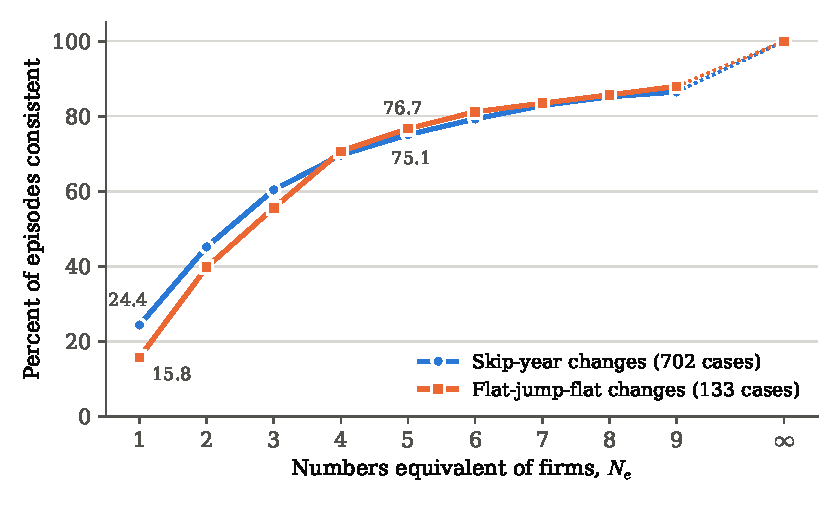
\includegraphics[width=0.78\textwidth]{figures/ch03/as_numbers_equivalent.pdf}
\caption{Share of tax-increase episodes consistent with a numbers equivalent $N_e$, from the bound
\eqref{eq:03-as-ne}. Only pairs with $\Delta q \le 0$ and $\Delta p \ge 0$ enter. At $N_e = \infty$ every
episode is consistent. The paper's table heads the second column ``Jump-Flat-Jump'', and its text calls the
sample flat-jump-flat. Redrawn from the numbers in \citet[Table III]{AshenfelterSullivan1987}.}
\label{fig:03-as-numbers}
\end{figure}

\casehead{Robustness} The authors probe the failures in four ways. First, 371 of the 1133 skip-year pairs
show price and quantity moving in the same direction, which signals a demand shift. Dropping them raises both
the output and the price predictions to 92 percent, while the revenue inequality holds in only 26 percent
(p.~493). Second, they allow for trends with a comparison group. In a simple version, the predicted change without a
tax change is the mean change in states that kept their statutory rate that year. In a two-way version, it is
the fit of a model with state and year effects to the state-years without a statutory change. The tests then ask whether quantity fell below, and price
rose above, these predictions. Their Table IV reports the results. With the simple fit, the quantity and price
predictions hold in 68.4 and 80.9 percent of the 288 consecutive-year statutory changes, and jointly in 60.1
percent. On the 199 flat-jump-flat pairs they hold in 68.8 and 92.0 percent, and jointly in 65.3 percent. The
two-way fit does better. On the statutory changes the shares are 77.8, 79.2 and 68.4 percent. On flat-jump-flat
pairs both predictions hold in 83.9 percent of cases, with 85.9 and 97.0 percent separately. The authors note the analogy with
program evaluation, where untreated units serve as controls \citep{Ashenfelter1978}. In modern terms this is a
difference-in-differences adjustment (\cref{app:econometrics}). Third, in nominal terms the price rises in 196
of the 199 flat-jump-flat pairs, though rising consumer prices make that success partly mechanical. Fourth,
they test whether tax increases follow particular movements in prices and quantities. Their sign-based
contingency tables condition on whether the tax rose in the previous year. The Pearson statistic is 3.9 when it
did not and 34.9 when it did, each with 3 degrees of freedom. The overall statistic is 38.8 with 6 degrees of
freedom. The second and the overall statistic rest on cells with very small expected counts, so the
$\chi^2$ approximation may be poor. Almost all of the 34.9 comes from the two cells in which price and quantity
both fell. The authors conclude that endogenous tax timing does not explain the failures (Table V,
pp.~495--496).

\casehead{Assessment} The test shows how far pure revealed preference can go, and it rejects monopoly
decisively. Its limits are instructive. The approach has no stochastic framework, a drawback the authors
acknowledge (n.~3). The percentages are therefore descriptive, and a single mismeasured pair can violate
\eqref{eq:03-as-revenue}. Quantities
inferred from tax receipts are suspect in exactly the years the test uses, because consumers and retailers
can stock up before a tax increase or buy across state lines. The maintained hypothesis of stable demand and
cost over one or two years is strong, as the frequent failures of the output and price predictions show.
Once a comparison group corrects for demand shifts, the test is no longer nonparametric, as the authors
concede (p.~494). Finally, a rejection of monopoly says little about which oligopoly model holds, beyond the
lower bound on $N_e$. The paper's lasting contribution is the idea of bounding conduct with inequalities
implied by optimization, which returns in \cref{sec:03-bounds}.

\subsection{Panzar and Rosse (1987): the revenue test}\label{sec:03-panzar-rosse}

\citet{PanzarRosse1987} propose two ideas \citep[pp.~1034--1035]{Bresnahan1989}. The first is to estimate a
reduced form and focus on the coefficients of factor prices. The second is to use revenue as the dependent
variable. Revenue is often observable when price and quantity are not. It also needs no quality correction,
whereas a price per unit can overstate the true price where the product is better. \Cref{sec:01-id-cost} previewed
the test. This section proves its properties.

\casehead{Setup} Firm $i$ produces output $q$ at cost $C(q, w, z)$, where $w = (w_1, \dots, w_K)$ is the
vector of factor prices and $z$ collects other cost shifters. Its revenue function is $R(q, y)$, with $y$ a
vector of demand shifters. Solving the equilibrium for the firm's revenue gives the \emph{reduced-form
revenue} $R^*(w, z, y)$. The \emph{Panzar-Rosse statistic} is the sum of the factor-price elasticities of
reduced-form revenue,
\begin{equation}\label{eq:03-pr-psi}
  \psi = \sum_{k=1}^{K} \frac{\partial R^*}{\partial w_k}\frac{w_k}{R^*}
       = \frac{\dd \ln R^*(\lambda w, z, y)}{\dd \lambda}\bigg|_{\lambda = 1},
\end{equation}
where the second equality follows from the chain rule. In words, $\psi$ is the percentage change in
equilibrium revenue after a 1 percent increase in all factor prices. \citet{Bresnahan1989} writes it $H_R$.
With a log-linear specification,
\begin{equation}\label{eq:03-pr-regression}
  \ln R_i = a + \sum_{k=1}^{K} \beta_k \ln w_{ki} + \gamma^\top x_i + e_i, \qquad \hat\psi = \sum_{k=1}^{K}
  \hat\beta_k ,
\end{equation}
where $x_i$ contains the other cost and demand shifters. Early applications either use such a
specification, which makes $\psi$ constant, or report $\psi$ near the center of the sample
\citep[n.~27]{Bresnahan1989}.

\begin{lemma}[Homogeneity of cost]\label{lem:03-homogeneity}
For a cost-minimizing firm and every $\lambda > 0$, $C(q, \lambda w, z) = \lambda C(q, w, z)$. Marginal cost
$C_q$ is also homogeneous of degree one in $w$, and $\sum_k w_k \frac{\partial C_q}{\partial w_k} = C_q$.
\end{lemma}

\begin{proof}
Scaling all factor prices by $\lambda$ leaves relative prices, and hence the cost-minimizing input bundle,
unchanged. Cost is therefore multiplied by $\lambda$. Differentiating $C(q, \lambda w, z) = \lambda C(q, w,
z)$ in $q$ gives $C_q(q, \lambda w, z) = \lambda C_q(q, w, z)$. Euler's theorem for functions homogeneous of
degree one gives the last statement.
\end{proof}

\begin{proposition}[Panzar and Rosse]\label{prop:03-panzar-rosse}
\leavevmode
\begin{enumerate}[label=(\roman*)]
  \item \emph{Monopoly.} If the firm is a monopolist, $\psi \le 0$. This holds also when it chooses a vector
  of outputs, qualities or advertising levels.
  \item \emph{Long-run competition.} Suppose free entry drives every active firm to the minimum of a U-shaped
  average cost curve. Then $\psi = 1$, and firm revenue does not depend on the demand shifters $y$.
  \item \emph{Chamberlinian competition.} Consider a symmetric free-entry equilibrium in which each firm
  maximizes profit against a downward-sloping demand. Suppose entry shifts that demand down and does not make
  it less elastic at a given output. Then $\psi \le 1$.
\end{enumerate}
\end{proposition}

\begin{proof}
\emph{(i), first proof: revealed preference.} Let $x$ be the vector of choices, with revenue $R(x)$ and cost
$C(x, w)$ homogeneous of degree one in $w$. Fix $w^0$ and $w^1 = \lambda w^0$ with $\lambda > 1$, and let $x^0$
and $x^1$ be the optimal choices. Optimality of $x^0$ at $w^0$ gives
\begin{equation*}
  R(x^0) - C(x^0, w^0) \ge R(x^1) - C(x^1, w^0)
  \quad\Longrightarrow\quad
  C(x^1, w^0) - C(x^0, w^0) \ge R(x^1) - R(x^0).
\end{equation*}
Optimality of $x^1$ at $w^1$, with $C(x, w^1) = \lambda C(x, w^0)$, gives
\begin{equation*}
  R(x^1) - R(x^0) \;\ge\; \lambda\bigl[C(x^1, w^0) - C(x^0, w^0)\bigr] \;\ge\; \lambda\bigl[R(x^1) -
  R(x^0)\bigr],
\end{equation*}
where the second step uses the first display. Hence $(1 - \lambda)[R(x^1) - R(x^0)] \ge 0$. Since $\lambda >
1$, $R(x^1) \le R(x^0)$. Equilibrium revenue cannot rise when all factor prices rise in proportion, so
$R^*(\lambda w^0) \le R^*(w^0)$ for $\lambda > 1$, and \eqref{eq:03-pr-psi} gives $\psi \le 0$.

\emph{(i), second proof: comparative statics.} With a single output, the monopolist's first-order condition
is $R_q(q^*, y) = C_q(q^*, w, z)$, and the second-order condition is $R_{qq} - C_{qq} < 0$. Differentiating the
first-order condition in $w_k$ gives
\begin{equation*}
  R_{qq}\frac{\partial q^*}{\partial w_k} = C_{qq}\frac{\partial q^*}{\partial w_k} + C_{q w_k}
  \quad\Longrightarrow\quad
  \frac{\partial q^*}{\partial w_k} = \frac{C_{q w_k}}{R_{qq} - C_{qq}} .
\end{equation*}
Equilibrium revenue is $R^* = R(q^*(w), y)$, so $\frac{\partial R^*}{\partial w_k} = R_q \frac{\partial
q^*}{\partial w_k}$. Multiply by $w_k$, sum over $k$, and apply \cref{lem:03-homogeneity} and then the
first-order condition:
\begin{equation*}
  \sum_k w_k \frac{\partial R^*}{\partial w_k}
  = \frac{R_q \sum_k w_k C_{q w_k}}{R_{qq} - C_{qq}}
  = \frac{R_q\, C_q}{R_{qq} - C_{qq}}
  = \frac{(R_q)^2}{R_{qq} - C_{qq}} .
\end{equation*}
Dividing by $R^*$ yields
\begin{equation}\label{eq:03-pr-monopoly}
  \psi = \frac{(R_q)^2}{(R_{qq} - C_{qq})\, R^*} \;\le\; 0,
\end{equation}
which is equation (23) of \citet{Bresnahan1989}. The inequality is strict when marginal cost is positive,
because then $R_q > 0$.

\emph{(ii)} Write average cost as $AC(q, w, z) = \frac{C(q, w, z)}{q}$. Each active firm produces at the output
$q^m(w, z)$ that minimizes it, and free entry sets the price equal to minimum average cost $MAC(w, z)$. By
\cref{lem:03-homogeneity}, $AC(q, \lambda w, z) = \lambda AC(q, w, z)$. Scaling by $\lambda$ does not move the
minimizer, so $q^m$ is homogeneous of degree zero in $w$, and $MAC$ is homogeneous of degree one. Firm revenue
$R^* = MAC(w, z)\, q^m(w, z)$ is then homogeneous of degree one in $w$, and Euler's theorem gives $\sum_k w_k
\frac{\partial R^*}{\partial w_k} = R^*$, that is, $\psi = 1$. Neither factor of $R^*$ involves $y$. A demand
shift changes the number of firms and leaves the revenue of each unchanged.

\emph{(iii)} Treat the number of firms $n$ as continuous. Each firm's revenue is $R(q, n)$ with $R_n < 0$,
since more rivals lower the price at which a given output sells. A symmetric equilibrium satisfies
$R_q(q, n) = C_q(q, w)$ and zero profit, $R(q, n) = C(q, w)$. Scale $w$ by $\lambda$ and differentiate both
conditions at $\lambda = 1$, using $C(q, \lambda w) = \lambda C(q, w)$:
\begin{align*}
  R_q\, \dd q + R_n\, \dd n &= C_q\, \dd q + C\, \dd\lambda, \\
  R_{qq}\, \dd q + R_{qn}\, \dd n &= C_{qq}\, \dd q + C_q\, \dd\lambda .
\end{align*}
Since $R_q = C_q$, the first line gives $R_n\, \dd n = C\, \dd\lambda$. The change in revenue is $\dd R^* = R_q\, \dd q +
R_n\, \dd n = C_q\, \dd q + C\, \dd\lambda$. Dividing by $R^* = C$ gives
\begin{equation*}
  \psi = 1 + \frac{C_q}{C}\,\frac{\dd q}{\dd\lambda},
\end{equation*}
so $\psi \le 1$ exactly when firm output does not rise. Substituting $\frac{\dd n}{\dd\lambda} = \frac{C}{R_n}$
into the second line gives
\begin{equation*}
  \frac{\dd q}{\dd\lambda} = \frac{C_q - \frac{R_{qn}}{R_n}\, C}{R_{qq} - C_{qq}} .
\end{equation*}
The denominator is negative by the second-order condition. So $\frac{\dd q}{\dd\lambda} \le 0$ if and only if $C_q
\ge \frac{R_{qn}}{R_n}C$. Use $C = R$ and $C_q = R_q$, divide by $R > 0$, and multiply by
$\frac{R_n}{R_q} < 0$. The condition becomes $\frac{R_n}{R} \le \frac{R_{qn}}{R_q}$, that is,
$\frac{\partial}{\partial n}\ln\frac{R_q}{R} \ge 0$. At a fixed $q$, $\frac{q R_q}{R} = 1 -
\frac{1}{\varepsilon_f}$, where $\varepsilon_f$ is the elasticity of the firm's demand. The condition
therefore says that entry does not lower $\varepsilon_f$.
\end{proof}

Part (iii) is Proposition~1 of \citet[p.~451]{PanzarRosse1987}. They assume that each firm's inverse demand
falls with its own output and with the number of rivals. Their Assumption~1 adds that the elasticity of each
firm's perceived demand is nondecreasing in the number of symmetric rivals (p.~450). The derivation above is
ours. Like theirs, it shows that the result rests on how entry changes the elasticity of each firm's demand.
When entry leaves $\varepsilon_f$ unchanged, firm output is fixed and $\psi = 1$, as in the long-run
competitive case. Panzar and Rosse also show that monopolistic competition, long-run competition and
conjectural-variation oligopoly are each consistent with $\psi > 0$ (p.~447). In their oligopoly model, $\psi$
has the sign opposite to that of industry marginal revenue. It is positive when industry output lies on the
inelastic part of market demand (pp.~454--455).

\begin{example}[Values of $\psi$ in standard models]\label{ex:03-pr-examples}
Let marginal cost be a constant $c(w)$, homogeneous of degree one in $w$, so that $\frac{\dd\ln c}{\dd\ln\lambda}
= 1$.
\begin{enumerate}[label=(\alph*)]
  \item Monopoly with demand $Q = AP^{-\varepsilon}$, $\varepsilon > 1$. The price is $P =
  \frac{\varepsilon}{\varepsilon - 1}c$ and revenue is $R^* = AP^{1 - \varepsilon}$, so $\psi = 1 -
  \varepsilon < 0$.
  \item Monopoly with demand $P = a - bQ$. Then $Q = \frac{a - c}{2b}$, $P = \frac{a + c}{2}$ and $R^* =
  \frac{a^2 - c^2}{4b}$, so $\psi = -\frac{2c^2}{a^2 - c^2} < 0$.
  \item Long-run competition with $C(q, w) = g(w)(f + q^2)$ and $g$ homogeneous of degree one. Average cost
  $g(w)(\frac{f}{q} + q)$ is minimized at $q^m = \sqrt{f}$, so $MAC = 2g(w)\sqrt{f}$, $R^* = 2g(w)f$ and
  $\psi = 1$.
  \item Short-run competition with $n$ fixed firms and rising marginal cost. Firm revenue is $\frac{P\,
  D(P)}{n}$, so $\psi = (1 - \varepsilon)\frac{\dd\ln P}{\dd\ln\lambda}$. Its sign is the sign of $1 -
  \varepsilon$.
  \item Cournot with $n$ fixed firms and demand $Q = AP^{-\varepsilon}$, $n\varepsilon > 1$. The Lerner
  index is $\frac{1}{n\varepsilon}$, so $P = \frac{n\varepsilon}{n\varepsilon - 1}c$. Firm revenue is
  $\frac{AP^{1 - \varepsilon}}{n}$, so $\psi = 1 - \varepsilon$, as under monopoly.
\end{enumerate}
\end{example}

Cases (d) and (e) show what the statistic cannot do. Short-run competition and oligopoly do not sign $\psi$,
and $\psi < 0$ arises without monopoly whenever demand is elastic. A negative $\hat\psi$ is therefore no proof
of monopoly, a ``false finding of monopoly'' in the words of \citet[p.~1036]{Bresnahan1989}. The usable
conclusions are one-sided. An estimate $\hat\psi > 0$ rejects monopoly. An estimate $\hat\psi < 1$ rejects
long-run competition, provided the markets are in long-run equilibrium. An estimate between zero and one
rejects both.

The specification matters as much as the sign. When the hypothesis is monopoly, $R^*$ depends on demand
shifters, and the revenue equation is misspecified if they are left out \citep[n.~28]{Bresnahan1989}. When
the hypothesis is long-run competition, demand shifters should have zero coefficients. This gives a second
testable restriction (p.~1037 and n.~30). Every factor price must be measured, and each must vary
exogenously. If a factor is omitted, $\hat\psi$ measures the response to only part of a proportional cost
increase. The long-run interpretation also requires that a cross-section of local markets reflects
differences in long-run equilibria. \citet{Rosse1970} addresses this with a ``permanent plant'' hypothesis,
and markets with rising demand should be treated separately from markets with falling demand
\citep[p.~1037]{Bresnahan1989}.

\casehead{Applications} The first applications use cross-sections of similar local markets, which suits the
long-run reading of the statistic. In a newspaper study, \citet{PanzarRosse1977} take each newspaper as an
observation, with its revenue, mostly from advertising, as the dependent variable. They reject monopoly
($\hat\psi > 0$) even for newspapers that are the only paper in their town. \citet[p.~1037]{Bresnahan1989} reads
this as evidence of competition from other media. In all but one specification the study also rejects $\psi = 1$,
and no specification rejects the Chamberlinian bound $\psi \le 1$. \citet[p.~453, n.~4]{PanzarRosse1987} call these
results suggestive rather than conclusive. \citet{Shaffer1982} applies the test to a cross-section of
banks in New York State in 1979. He rejects both monopoly and long-run competition (p.~1037). The test also bears on market definition. A rejection of monopoly for a firm or a
group of firms means they cannot be treated as acting in isolation \citep[p.~1050]{Bresnahan1989}.

\casehead{Assessment} The revenue test asks little of the data on endogenous variables and makes no
assumption about functional forms. Its demands lie elsewhere. It needs the full vector of factor prices with
exogenous variation in each, and its sharpest prediction ($\psi = 1$) requires long-run equilibrium with free
entry. Like the two tests before it, it delivers inequalities. All three reject monopoly or cartel pricing in
their applications, and none of them says how much market power remains.

\section{Residual demand: Baker and Bresnahan (1988)}\label{sec:03-residual-demand}

\subsection{The question and the idea}\label{sec:03-rd-idea}

The tests so far treat the product as homogeneous and ask about industry conduct. Most industries sell
differentiated products, and then a firm's market power depends on substitution as well as on behavior. A
firm with a unique product can have substantial power, while a firm whose rival sells a near-identical
product may have almost none. Measuring this with a full demand system is costly. Even with constant
elasticities and symmetry, $N$ products require $N$ own-price elasticities, $N$ income elasticities and
$\frac{N(N - 1)}{2}$ cross-price elasticities \citep[p.~1045]{Bresnahan1989}. With 100 products that is more
than 5,000 parameters.

\citet{BakerBresnahan1988} estimate one equation per firm instead. The \emph{residual demand curve} of a firm
is the relation between its own price and quantity after accounting for the supply response of all other
firms (p.~284). A firm in a perfectly competitive industry faces a flat residual demand curve. A monopolist's
residual demand is the industry demand. A firm selling a differentiated product lies in between.
\Cref{fig:03-residual-demand} draws the construction for a homogeneous good. The slope of residual demand
summarizes market power without identifying its source.

\subsection{Deriving the residual demand curve}\label{sec:03-rd-model}

Firm 1 is the firm of interest and sells a single product. Let $\mathbf{Q} = (Q_2, \dots, Q_N)$ be the
quantities of all other relevant products, including products of firms in other ``industries''. No market
is defined in advance. Let $Y$ be demand shifters, $W$ industry-wide cost shifters, and $W^i$ cost shifters
specific to firm $i$. The model has four blocks \citep[pp.~286--289]{BakerBresnahan1988}. Firm 1's inverse
demand is
\begin{equation}\label{eq:03-bb-demand1}
  P_1 = P^1(Q_1, \mathbf{Q}, Y).
\end{equation}
When all products are identical it reduces to $P_1 = P^1(Q_1 + \sum_{i \neq 1} Q_i, Y)$, and only then are
market definition and demand estimation straightforward. The rivals' inverse demands are
\begin{equation}\label{eq:03-bb-demand-others}
  P_i = P^i(\mathbf{Q}, Q_1, Y), \qquad i \neq 1 .
\end{equation}
Each rival's supply relation sets marginal cost equal to perceived marginal revenue,
\begin{equation}\label{eq:03-bb-supply-others}
  MC^i(Q_i, W, W^i) = P^i(\cdot) + Q_i \sum_j \frac{\partial P^i}{\partial Q_j}\frac{\partial Q_j}{\partial
  Q_i}, \qquad i \neq 1,
\end{equation}
where the conjectures $\frac{\partial Q_j}{\partial Q_i}$ are indexed by conduct parameters $\theta^i$, as in
\cref{sec:03-framework}. The firm-specific shifters $W^i$ do not appear in $W$. They may be local input prices
or the shadow rental value of an asset the firm does not trade.

Solve the $2(N - 1)$ equations \eqref{eq:03-bb-demand-others} and \eqref{eq:03-bb-supply-others} for the
rivals' prices and quantities, holding $Q_1$ fixed. Write $W^I$ for the collection of the rivals' shifters
$W^i$. The solution for quantities is the \emph{partial reduced form}
\begin{equation}\label{eq:03-bb-partial-rf}
  \mathbf{Q} = E^I(Q_1, Y, W, W^I),
\end{equation}
in which $Q_1$ is the only endogenous variable on the right. Let $e_{i1} = \frac{\partial \ln E^i}{\partial
\ln Q_1}$ be the elasticity of rival $i$'s equilibrium quantity with respect to $Q_1$. Substituting
\eqref{eq:03-bb-partial-rf} into \eqref{eq:03-bb-demand1} gives the residual inverse demand of firm 1,
\begin{equation}\label{eq:03-residual-demand}
  P_1 = P^1\bigl(Q_1, E^I(Q_1, Y, W, W^I), Y\bigr) \equiv R(Q_1, Y, W, W^I).
\end{equation}
Its observable arguments are own quantity, demand shifters and the cost shifters of other firms. Its
parameters mix demand, cost and conduct parameters, and they cannot in general be recovered from it.

The elasticity of an inverse demand function is called a \emph{flexibility}. Let $\eta_{1j} = \frac{\partial
\ln P^1}{\partial \ln Q_j}$ be the flexibilities of firm 1's structural inverse demand. Differentiate the log
of \eqref{eq:03-residual-demand} in $\ln Q_1$ by the chain rule:
\begin{equation}\label{eq:03-bb-elasticity}
  \eta^R_1 \equiv \frac{\partial \ln R}{\partial \ln Q_1}
  = \frac{\partial \ln P^1}{\partial \ln Q_1} + \sum_{i \neq 1}\frac{\partial \ln P^1}{\partial \ln Q_i}
    \frac{\partial \ln E^i}{\partial \ln Q_1}
  = \eta_{11} + \sum_{i \neq 1} \eta_{1i}\, e_{i1}.
\end{equation}
This is equation (7) of the paper.\footnote{The printed equation (7) writes the reaction elasticity with the
indices in the order $1i$. The definition two lines above it, which we follow, is $\frac{\partial \ln
E^i}{\partial \ln Q_1}$.} The \emph{inverse residual demand elasticity} $\eta^R_1$ is the parameter to be
estimated, and $\frac{1}{\eta^R_1}$ is the elasticity of residual demand. The first term is the own
flexibility. The second adds the price effect of the rivals' responses. With homogeneous products and
rivals that expand when firm 1 contracts, the second term partly offsets the first. In the competitive limit
the two cancel.

Firm 1's own supply relation closes the model:
\begin{equation}\label{eq:03-bb-supply1}
  P_1 - MC^1(Q_1, W, W^1) = M^1(\mathbf{Q}, Q_1, Y, \theta^1) = MK^1(Q_1, Y, W, W^I, \theta),
\end{equation}
where $M^1$ is the gap between price and perceived marginal revenue. The second equality substitutes
\eqref{eq:03-bb-partial-rf} for $\mathbf{Q}$, and \citet{BakerBresnahan1988} call $MK^1$ the \emph{residual
markup}. The intersection of \eqref{eq:03-residual-demand} and \eqref{eq:03-bb-supply1} determines $P_1$
and $Q_1$.

\casehead{Identification} Equations \eqref{eq:03-residual-demand} and \eqref{eq:03-bb-supply1} form a
two-equation simultaneous system in $(P_1, Q_1)$. The shifters $Y$, $W$ and $W^I$ enter both equations.
Firm 1's own cost shifter $W^1$ enters only the supply relation. It is therefore the excluded instrument for
$Q_1$ in the residual demand curve (p.~289). The order condition requires at least one firm-specific cost
shifter. The rank condition requires that firm 1's costs move independently of the costs of all other firms
\citep[n.~43]{Bresnahan1989}. Bresnahan suggests exchange rates as a natural experiment for producers in a
single country, since they move real costs across countries. Industry-wide cost shifters cannot serve,
because they shift the residual demand curve itself.

This is the central contrast with \cref{sec:03-sumner} and \cref{sec:03-sullivan}. A tax moves every firm's
marginal cost together. It therefore traces out market demand and speaks to industry conduct. A cost shifter
specific to one firm moves that firm's supply relation alone. It traces out the firm's residual demand and
speaks to the firm's market power.

\begin{example}[Dominant firm with a price-taking fringe]\label{ex:03-dominant-fringe}
Let products be homogeneous and let the rivals be price takers with supply $S(P, W, W^I)$. Firm 1's residual
demand is $Q_1 = D(P, Y) - S(P, W, W^I)$. Write $\varepsilon$ for the market demand elasticity,
$\varepsilon_S$ for the fringe supply elasticity and $s_1 = \frac{Q_1}{D}$ for firm 1's share. Differentiating
gives the residual demand elasticity
\begin{equation*}
  \varepsilon^R = -\frac{\partial Q_1}{\partial P}\frac{P}{Q_1}
  = \frac{\varepsilon D + \varepsilon_S S}{Q_1}
  = \frac{\varepsilon}{s_1} + \varepsilon_S\,\frac{1 - s_1}{s_1},
\end{equation*}
the familiar formula of \citet{LandesPosner1981}. Here $\eta^R_1 = -\frac{1}{\varepsilon^R}$. With no
fringe, $s_1 = 1$ and $\varepsilon^R = \varepsilon$. With a fringe whose marginal cost is flat,
$\varepsilon_S = \infty$ and residual demand is flat at the fringe's cost \citep[p.~1049]{Bresnahan1989}.

A linear case verifies the markup property proved below. Let $D = a - bP$, $S = dP$ and let firm 1 have
constant marginal cost $c$. Residual demand is $Q_1 = a - (b + d)P$, or $P = \frac{a - Q_1}{b + d}$. The
dominant firm's optimum is $Q_1 = \frac{a - (b + d)c}{2}$, which gives $P - c = \frac{Q_1}{b + d}$. Hence
\begin{equation*}
  \frac{P - c}{P} = \frac{Q_1}{a - Q_1} = -\frac{\partial \ln P}{\partial \ln Q_1} = -\eta^R_1 .
\end{equation*}
\end{example}

\begin{figure}[htbp]
\centering
\begin{tikzpicture}[scale=0.62, >=Stealth]
  \draw[->] (0,0) -- (11.2,0) node[below left] {quantity};
  \draw[->] (0,0) -- (0,11) node[above right] {price $P$};
  \draw[very thick] (0,10) -- (10,0) node[pos=0.06, right=2pt] {$D$};
  \draw[thick, blue!60!black] (0,2) -- (8.5,10.5) node[above] {$S_R$};
  \draw[very thick, red!70!black] (0,6) -- (8,2) -- (10,0);
  \node[red!70!black, anchor=south west] at (0.25,6.2) {$D^R$};
  \draw[thick, dashed, gray!70!black] (0,2) -- (8,2);
  \node[gray!30!black, anchor=west, align=left, font=\small] (flat) at (9.2,3.4)
     {flat $D^R$ when rivals'\\ marginal cost is flat};
  \draw[->, gray!30!black] (flat.south west) -- (7.4,2.1);
  \draw[dotted] (0,4) -- (6,4);
  \node[left] at (0,4) {$\bar P$};
  \fill (2,4) circle (2.5pt) (4,4) circle (2.5pt) (6,4) circle (2.5pt);
  \draw[dotted] (2,0) -- (2,4) (4,0) -- (4,4) (6,0) -- (6,4);
  \node[below, font=\scriptsize] at (2,0) {$S_R(\bar P)$};
  \node[below, font=\scriptsize] at (4,0) {$D^R(\bar P)$};
  \node[below, font=\scriptsize] at (6,0) {$D(\bar P)$};
\end{tikzpicture}
\caption{Residual demand. At each price $\bar P$ the residual demand of firm 1 is market demand minus the
quantity rivals supply, $D^R(\bar P) = D(\bar P) - S_R(\bar P)$. A monopolist faces $D$ itself. If rivals can
expand at a flat marginal cost, residual demand is flat at that cost (dashed). Upward-sloping rival supply
produces an intermediate slope. Drawn for $D$: $P = 10 - Q$ and $S_R$: $P = 2 + Q$, which give $D^R$: $P = 6 -
\frac{Q_1}{2}$ above the price 2.}
\label{fig:03-residual-demand}
\end{figure}

\subsection{When the residual demand slope measures the markup}\label{sec:03-rd-markup}

A firm with a flat residual demand curve cannot raise its price, so $\eta^R_1 < 0$ implies $P_1 > MC_1$
(p.~289). The exact relation between $\eta^R_1$ and the Lerner index depends on conduct.

\begin{proposition}[Baker and Bresnahan]\label{prop:03-rd-markup}
Firm 1's Lerner index equals the negative of its inverse residual demand elasticity,
\begin{equation}\label{eq:03-bb-markup}
  \frac{P_1 - MC_1}{P_1} = -\eta^R_1,
\end{equation}
in each of the following cases. (a) Firm 1 is a Stackelberg leader relative to its environment, so that it
chooses $Q_1$ knowing that rivals respond along $E^I$. A dominant firm facing a price-taking fringe is the
leading example. (b) Firms are in a consistent-conjectures equilibrium \citep{Bresnahan1981a}, in which firm
1's conjectured reaction elasticities equal the true ones. (c) The industry is perfectly competitive.
\end{proposition}

\begin{proof}
(a) Firm 1 maximizes $R(Q_1, Y, W, W^I)\, Q_1 - C_1(Q_1)$. The first-order condition is $R + Q_1
\frac{\partial R}{\partial Q_1} = MC_1$. Divide by $P_1 = R$:
\begin{equation*}
  1 + \eta^R_1 = \frac{MC_1}{P_1}
  \quad\Longleftrightarrow\quad
  \frac{P_1 - MC_1}{P_1} = -\eta^R_1 .
\end{equation*}
(b) Let $\hat e_{i1}$ be firm 1's conjectured elasticity of $Q_i$ with respect to $Q_1$. Its perceived
marginal revenue is
\begin{equation*}
  \frac{\dd (P^1 Q_1)}{\dd Q_1}
  = P^1 + Q_1\Bigl[\frac{\partial P^1}{\partial Q_1} + \sum_{i \neq 1}\frac{\partial P^1}{\partial Q_i}
    \frac{\dd Q_i}{\dd Q_1}\Bigr]
  = P^1\Bigl[1 + \eta_{11} + \sum_{i \neq 1}\eta_{1i}\,\hat e_{i1}\Bigr].
\end{equation*}
Equating it to $MC_1$ gives $\frac{P_1 - MC_1}{P_1} = -(\eta_{11} + \sum_{i \neq 1}\eta_{1i}\hat e_{i1})$,
which is equation (11) of the paper. Consistency means $\hat e_{i1} = e_{i1}$, and then the right side equals
$-\eta^R_1$ by \eqref{eq:03-bb-elasticity}. (c) Under perfect competition rivals absorb any change in $Q_1$ at
an unchanged price, so $\eta^R_1 = 0$, and price equals marginal cost.
\end{proof}

Product differentiation gives an approximate version. When products are poor substitutes, the cross
flexibilities $\eta_{1i}$ are small. Then $\eta^R_1 \approx \eta_{11}$, and the markup under any conjecture is
close to $-\eta_{11}$. Questions about strategic variables disappear in this limit \citep{Sonnenschein1968}.
\citet[p.~290]{BakerBresnahan1988} conclude that a large $-\eta^R_1$ will generally indicate substantial
market power for firms selling differentiated products. Outside these cases the equality can fail, as the
next example shows.

\begin{example}[Cournot competition: residual demand understates the markup]\label{ex:03-cournot-residual}
Let $P = a - Q$ and let $N$ identical Cournot firms have marginal cost $c$. Rival $j$'s best response is $q_j
= \frac{a - c - Q_{-j}}{2}$. Given $Q_1$, symmetric rivals each produce $q$ with $2q = a - c - Q_1 - (N -
2)q$, so $q = \frac{a - c - Q_1}{N}$. Substituting into demand gives the residual inverse demand
\begin{equation*}
  P = a - Q_1 - (N - 1)\frac{a - c - Q_1}{N} = \frac{a + (N - 1)c}{N} - \frac{Q_1}{N}.
\end{equation*}
At the Cournot equilibrium $Q_1 = \frac{a - c}{N + 1}$ and $P = \frac{a + Nc}{N + 1}$, a point on this curve.
The Lerner index is $L = \frac{a - c}{a + Nc}$. The inverse residual demand elasticity is
\begin{equation*}
  -\eta^R_1 = \frac{1}{N}\cdot\frac{Q_1}{P} = \frac{a - c}{N(a + Nc)} = \frac{L}{N} .
\end{equation*}
A Cournot firm takes rivals' outputs as given, while its residual demand incorporates their responses. With
strategic substitutes the rivals' contraction absorbs part of the price effect, so $-\eta^R_1$ understates the
markup by the factor $N$.
\end{example}

\subsection{The brewing application}\label{sec:03-bb-brewing}

\casehead{Setting} \citet{BakerBresnahan1988} estimate the residual demand curves of Anheuser-Busch (A-B),
Pabst and Coors over 1962--1982. The industry has substantial product differentiation, and no satisfactory
estimates of its demand and cross elasticities existed. Antitrust enforcers suspected market power and
blocked several proposed mergers (p.~285). A-B was the largest brewer throughout. Its share of national unit
sales rose from under 10 percent to over 30 percent, overwhelmingly through internal growth. Pabst held 7.5 to
11.5 percent of national sales over the last decade of the sample. Its regional share was much higher, about a
quarter of dollar sales in the East North Central states during the 1970s. Coors was slightly smaller than
Pabst nationally. It had the largest share in each of ten western states, averaging about 40 percent in the
mountain states and nearly 30 percent in the Pacific states (pp.~290--291). Coors brewed in a single plant in
Golden, Colorado, the largest in the industry, while A-B had ten plants. Miller's national marketing of light
beer from 1975 changed product differentiation in the industry and possibly the nature of competition.

\casehead{Data} The data are annual for 1962--1982, so each equation has 21 observations.
Price $p_j$ is the log of real average revenue, beer revenue divided by gallons sold, with revenue taken from
firm annual reports. Quantity $q_j$ is the log of per capita barrels, using the U.S. population over 18.
Monetary values are deflated by the GNP deflator. As a robustness check, the authors use the price of each firm's flagship brand
in northern California (Budweiser, Coors and Pabst Blue Ribbon). Average revenue could understate market power
if brand composition changes. The flagship prices are highly correlated with firm average revenue, at 0.96,
0.94 and 0.99 for the three firms. Correlations of average revenue across firms are lower, 0.82 for A-B and
Coors, 0.93 for A-B and Pabst, and 0.65 for Coors and Pabst (Table 1).

\casehead{Estimating equation} The authors estimate \eqref{eq:03-residual-demand} in double-log form for
each firm $j$, so that coefficients are elasticities. With lower-case letters for logs, their equation
(6$''$) is
\begin{equation}\label{eq:03-bb-estimating}
  p_j = \eta^R_j\, q_j + \delta_j^\top (w, w_I) + \gamma_j^\top y + u_j ,
\end{equation}
where $\delta_j$ and $\gamma_j$ are local symbols for coefficient vectors and $u_j$ is the error. Industry
costs $w$ consist of the log of real short-run average variable cost (\textit{sravc}), average industry plant
size (\textit{APS}) and the log of the real user cost of capital (\textit{pk}). Short-run average variable cost
summarizes all non-capital factor prices. The rivals' firm-specific costs $w_I$ are summarized by their excess capacity
$\mathit{EKTI}_j$. The demand shifters $y$ are log real per capita disposable income (\textit{pcdi}), a
time trend (\textit{TIME}) and a dummy for 1975 and later (\textit{LITE}). Advertising and two demographic
variables were tested and dropped. In the A-B equation the slope is $\eta^R_j + \eta^{LITE}\cdot \mathit{LITE}$, so the
interaction coefficient measures the change in slope after 1975. To save degrees of freedom, the three
equations share one index of rivals' marginal cost. This is the cross-equation restriction (12),
\begin{equation}\label{eq:03-bb-restriction}
  \delta_{1j}\, \mathit{sravc} + \delta_{2j}\mathit{APS} + \delta_{3j}\, \mathit{pk} + \delta_{4j}\mathit{EKTI}
  = \delta_j\bigl(\mathit{sravc} + \beta_{APS}\mathit{APS} + \beta_{PK}\, \mathit{pk} +
  \beta_{EKTI}\mathit{EKTI}\bigr) \equiv \delta_j\, \mathit{MC},
\end{equation}
with $\beta_{APS}$, $\beta_{PK}$ and $\beta_{EKTI}$ common to all firms (again local symbols). It assumes that
the other firms use inputs in the same proportions. Tests do not reject it, though they have little power
(n.~21).

\casehead{Instruments} Two variables on the right of \eqref{eq:03-bb-estimating} are endogenous. Short-run
average variable cost is endogenous if short-run marginal cost rises with output. It is instrumented by
exogenous factor prices, namely the brewing wage and the materials and advertising price indices
(\textit{pl}, \textit{pm}, \textit{pa}). Own quantity is endogenous because of the supply relation
\eqref{eq:03-bb-supply1}. All its instruments proxy for firm-specific factor prices $W^1$ (p.~293). The first
is the firm's per capita capacity $K_j$. Brewing capacity is altered infrequently and in large increments. A-B, with a quarter to a third of national sales, typically added
capacity in steps of about 20 percent of its annual production. Short-run marginal cost is therefore lowest
just after an expansion and highest just before the next one. Excess capacity would track this cycle too, but
it is endogenous even in the short run and is not used. The second instrument is the firm's average plant
size $\mathit{APS}_j$ for the multiplant firms A-B and Pabst, which tracks plant-level scale economies. For
Coors it is the log real Colorado manufacturing wage (\textit{cw}). The national brewing wage is already
among the industry cost variables, so independent movements in Colorado wages shift Coors's costs alone
(p.~294).

\casehead{Estimator} The three equations are estimated jointly by three-stage least squares. Stack them as $y
= X b + u$ and let $P_Z = Z(Z^\top Z)^{-1}Z^\top$ project on the instruments. Let $\hat\Sigma$ be the $3
\times 3$ covariance matrix of first-round two-stage least squares residuals. Without restrictions the
estimator is
\begin{equation*}
  \hat b_{3SLS} = \bigl[X^\top(\hat\Sigma^{-1} \otimes P_Z)X\bigr]^{-1} X^\top(\hat\Sigma^{-1} \otimes P_Z)\, y .
\end{equation*}
Restriction \eqref{eq:03-bb-restriction} makes the coefficients products of parameters, such as $\delta_j
\beta_{APS}$. The estimator then minimizes $u(b)^\top(\hat\Sigma^{-1} \otimes P_Z)u(b)$ over the restricted
parameters (\cref{app:econometrics}). Joint estimation uses the correlation of errors across equations, and
single-equation two-stage least squares gives similar elasticities with little loss of efficiency (n.~20). The
reported specification drops demand variables whose coefficients are smaller than their standard errors.
This removes the demographic variables, keeps \textit{LITE} only for A-B, and keeps \textit{TIME} only for
Pabst and Coors. Cost variables are kept even when insignificant, for a reason the next proposition makes
clear.

\casehead{What ordinary least squares would do} Suppose no firm-specific cost shifter were available. The
authors argue that ordinary least squares would then be biased toward finding no market power (p.~298). A
linear version of the system shows why and when.

\begin{proposition}[Bias of least squares in residual demand]\label{prop:03-ols-residual}
Let residual demand be $p = \eta q + u$ with $\eta \le 0$, and let the supply relation be $p = \lambda q +
\gamma w_1 + v$, with $\lambda > \eta$ and $\gamma \neq 0$. Let $w_1$ be uncorrelated with $(u, v)$, and write
$\sigma_u^2$, $\sigma_v^2$, $\sigma_{uv}$ and $\sigma_w^2$ for the variances and the covariance. Then
\begin{equation}\label{eq:03-ols-bias}
  \plim \hat\eta_{OLS} = \eta + (\lambda - \eta)\,
  \frac{\sigma_u^2 - \sigma_{uv}}{\sigma_u^2 + \sigma_v^2 - 2\sigma_{uv} + \gamma^2\sigma_w^2},
\end{equation}
while instrumental variables with instrument $w_1$ is consistent for $\eta$. If $\sigma_{uv} = 0$, the
least squares limit is the weighted average $(1 - \omega)\eta + \omega\lambda$ with $\omega =
\frac{\sigma_u^2}{\sigma_u^2 + \sigma_v^2 + \gamma^2\sigma_w^2} \in [0, 1)$.
\end{proposition}

\begin{proof}
Equate the two equations and solve for the equilibrium quantity:
\begin{equation*}
  q = \frac{u - v - \gamma w_1}{\lambda - \eta}.
\end{equation*}
Hence $\Cov(q, u) = \frac{\sigma_u^2 - \sigma_{uv}}{\lambda - \eta}$ and $\Var(q) = \frac{\sigma_u^2 +
\sigma_v^2 - 2\sigma_{uv} + \gamma^2\sigma_w^2}{(\lambda - \eta)^2}$. Least squares converges to $\eta +
\frac{\Cov(q, u)}{\Var(q)}$, which is \eqref{eq:03-ols-bias}. For the instrumental variables estimator,
$\Cov(w_1, q) = -\frac{\gamma\sigma_w^2}{\lambda - \eta} \neq 0$ and $\Cov(w_1, p) = \eta\Cov(w_1, q)$, so
their ratio is $\eta$. Setting $\sigma_{uv} = 0$ in \eqref{eq:03-ols-bias} gives the weighted average.
\end{proof}

With uncorrelated shocks, least squares lands between the residual demand slope and the supply slope. If the
supply relation is flat or rising, $\lambda \ge 0$, the estimate is pulled toward a flat residual demand. That
direction is conservative, since it understates market power. The proposition also shows when the argument
fails. A covariance $\sigma_{uv}$ above $\sigma_u^2$ reverses the sign of the bias. Omitted industry cost
variables create such a positive covariance, because they enter both equations. This is why the authors keep
all cost variables (n.~23).

\subsection{Results}\label{sec:03-bb-results}

\Cref{tab:03-baker-bresnahan} reproduces the paper's Table 3. The coefficient on log quantity is $\eta^R_j$.

\begin{table}[htbp]
\centering
\caption{Baker and Bresnahan (1988): residual demand estimates, three-stage least squares}
\label{tab:03-baker-bresnahan}
\begin{tabular}{lcccccc}
\toprule
 & \multicolumn{2}{c}{Anheuser-Busch} & \multicolumn{2}{c}{Pabst} & \multicolumn{2}{c}{Coors} \\
\cmidrule(lr){2-3}\cmidrule(lr){4-5}\cmidrule(lr){6-7}
Variable & Coef. & (s.e.) & Coef. & (s.e.) & Coef. & (s.e.) \\
\midrule
Constant & 2.113 & (0.505) & 3.979 & (0.362) & $-1.638$ & (0.805) \\
Own log quantity $q_j$ & $-0.312$ & (0.064) & $-0.058$ & (0.031) & $-0.745$ & (0.054) \\
$\mathit{LITE} \times q_{AB}$ & 0.282 & (0.040) & & & & \\
\textit{LITE} & 0.591 & (0.068) & & & & \\
\textit{PCDI} & 0.040 & (0.157) & $-0.041$ & (0.132) & 0.440 & (0.306) \\
\textit{MC} index & 0.278 & (0.019) & 0.107 & (0.089) & 0.266 & (0.226) \\
\textit{TIME} & & & $-0.017$ & (0.004) & 0.032 & (0.010) \\
\addlinespace
\multicolumn{7}{l}{\textit{Common parameters of the MC index}} \\
\textit{APS} & \multicolumn{6}{l}{$-0.194$ (0.291)} \\
\textit{PK} & \multicolumn{6}{l}{0.042 (0.115)} \\
\textit{EKTI} & \multicolumn{6}{l}{$-0.033$ (0.022)} \\
\addlinespace
Durbin-Watson & 2.13 & & 1.95 & & 1.70 & \\
Observations & 21 & & 21 & & 21 & \\
\bottomrule
\end{tabular}

\smallskip
\begin{minipage}{0.95\textwidth}
\footnotesize Notes: Reproduced from \citet[Table 3]{BakerBresnahan1988}. Dependent variable: log real
average revenue of the firm, 1962--1982. Estimates impose restriction \eqref{eq:03-bb-restriction}. The
\textit{MC} row reports $\delta_j$ and the common parameters report $\beta_{APS}$, $\beta_{PK}$ and
$\beta_{EKTI}$. Treating quantity as exogenous gives own-quantity coefficients of $-0.312$ (A-B),
$-0.053$ (Pabst) and $-0.738$ (Coors) (n.~26).
\end{minipage}
\end{table}

Under the markup reading of \cref{prop:03-rd-markup}, the estimates sort the three firms sharply. Coors's
coefficient of $-0.745$ has a $t$-statistic of $\frac{0.745}{0.054} \approx 13.8$. The authors read it as a
74 percent markup over marginal cost (p.~295). Strictly, $-\eta^R_1$ is a Lerner index, a margin as a share
of price. A Lerner index of 0.745 means $\frac{P}{MC} = \frac{1}{1 - 0.745} \approx 3.9$, a markup over cost
of about 290 percent (\cref{sec:03-objects}). A-B's coefficient before 1975 is $-0.312$, with $t \approx 4.9$
and $\frac{P}{MC} \approx 1.45$.

After 1975 A-B's coefficient is $-0.312 + 0.282 = -0.030$. The paper does not report the covariance of the
two estimates, so the standard error of the sum is unknown. It can still be bounded. For any correlation the
variance of a sum is at least $(0.064 - 0.040)^2$, so the standard error is at least 0.024. The
$t$-statistic for a flat residual demand after 1975 is therefore at most $\frac{0.030}{0.024} = 1.25$.
Competition cannot be rejected for A-B after 1975 at conventional levels, whatever the covariance.

Pabst's coefficient is $-0.058$ with $t \approx 1.87$, which the authors call insignificant. They report a 95
percent confidence interval for the markup of 1 to 11 percent (p.~296). The reported standard error implies
a two-sided 95 percent interval of $-0.058 \pm 1.96 \times 0.031$, or about $-0.3$ to 11.9 percent. The
interval of 1 to 11 percent corresponds to $\pm 1.645$ standard errors, a two-sided 90 percent interval. A
two-sided test at 5 percent therefore does not reject a flat residual demand for Pabst. With 21 observations,
using a $t$ distribution in place of the normal would make a rejection even less likely.

The other coefficients have no clean structural reading, since each mixes direct demand effects with the
indirect effects of rivals' adjustments \citep[p.~297]{BakerBresnahan1988}. The positive income coefficient
for Coors means that a rise in income shifts sales toward Coors after all rivals adjust. The authors label
Coors a normal good and Pabst an inferior good in residual demand. Real prices trend down by 1.7 percent a
year for Pabst and up by 3.2 percent a year for Coors, holding the other variables fixed. The Durbin-Watson
statistics of 1.70 to 2.13 show no strong first-order serial correlation in the double-log specification.

The least squares estimates in the note to \cref{tab:03-baker-bresnahan} confirm the sign of
\cref{prop:03-ols-residual}. They are slightly closer to zero than the instrumental variables estimates for
Coors and Pabst and identical for A-B. The bias is small, and the authors note that treating quantity as
endogenous matters little in their data (n.~19).

\subsection{Robustness, interpretation and critiques}\label{sec:03-bb-critique}

\casehead{Robustness} Using flagship-brand prices and quantities leaves the elasticity estimates unchanged
(p.~293). A linear specification evaluated at sample means gives the same qualitative pattern. It shows
somewhat less market power for A-B early in the sample and for Coors overall, and the two sets of
elasticities are not statistically different under an assumption of independence. The authors prefer the
double-log form because the linear errors are strongly serially correlated (pp.~296--297). Demand elasticity
results are robust to imposing restriction \eqref{eq:03-bb-restriction} (n.~21).

\casehead{Interpretation} The authors draw four inferences (p.~297). First, product differentiation is
important, and the steep residual demands of Coors and A-B probably come from products distinct in image and
geography. Second, regional market share is a poor guide to market power, since Pabst had high regional
shares and almost no power. Third, rising concentration and differentiation after 1975 reflect competition.
A-B lost most of its market power after Miller's light beer, although the new product apparently raised the
demand for all beer. Fourth, tacit collusion is unlikely. Under collusion every firm's residual demand would
slope down and prices would move closely together. Pabst shows neither. The authors concede that they cannot
reject the unlikely case in which all firms except Pabst collude to raise prices to the level of Pabst, the
high-cost producer (n.~25).

\casehead{Critiques} The markup reading requires one of the special cases of \cref{prop:03-rd-markup}. In
Cournot-like competition \cref{ex:03-cournot-residual} shows that $-\eta^R_1$ understates the markup, by a
factor of $N$ in the linear case. The authors themselves call the exact quantitative reading possibly too
strong (p.~297). The instruments raise their own questions. Capacity is added in anticipation of growth
(p.~293), so it may correlate with expected demand. The Colorado wage could move with western incomes and
hence with demand for Coors. The sample has 21 annual observations, and the specification was chosen by
dropping variables with $|t| < 1$, so reported standard errors ignore the search. National average revenue
also aggregates regional markets in which the three firms held very different positions. The light-beer dummy
is collinear with a surge in industry advertising in the mid-1970s, so its meaning is uncertain (n.~16).
Finally, the evidence against collusion leans on Pabst. Its price correlates at only 0.65 with Coors's, yet
at 0.93 with A-B's (Table 1).

\casehead{Contribution} The paper made firm-level market power measurable with one equation and modest data.
It separated two kinds of cost variation. Market-wide shifters identify market demand and industry conduct,
while firm-specific shifters identify a firm's residual demand. In Bresnahan's words, the residual demand
elasticity ``summarizes the market power of the firm'' but is ``insufficient to determine the sources of that
market power'' \citep[p.~1049]{Bresnahan1989}.

\subsection{Residual demand, market definition and mergers}\label{sec:03-bb-antitrust}

Residual demand applies equally to a group of firms \citep[n.~7]{BakerBresnahan1988}. This matters for
antitrust. A hypothetical cartel price increase of 5 percent is part of the algorithm that defines a market
under the 1984 Merger Guidelines of the U.S. Department of Justice. The residual demand of a candidate group
of firms speaks to that question directly. \citet{ScheffmanSpiller1987} extend the method in this way to
define geographic markets. The question of a group's market power is well posed even where defining a
relevant market and computing shares in it would be senseless \citep[n.~44]{Bresnahan1989}. \citet{BakerBresnahan1985} use the same tools to estimate the gains
from merger in differentiated industries. They ask how much steeper the residual demand of two firms would
be after a merger \citep[p.~1050]{Bresnahan1989}. If the two products are close substitutes and few others
are similar, each provides much of the competitive brake on the other. The steepening of the joint residual
demand measures the loss of that brake. These ideas return in \cref{ch:mergers}, and residual demand with a
full system of differentiated products is the subject of \cref{ch:diffprod}.

The studies in this section and the last share a pattern. Sullivan rejects cartel pricing in cigarettes, and
Ashenfelter and Sullivan find that only conduct with a moderate amount of competition fits the data. Panzar and
Rosse reject monopoly for newspapers, and Shaffer rejects both monopoly and long-run competition for banks. Baker
and Bresnahan place
three brewers between price taking and
substantial power. Most estimates of this generation fall between competition and monopoly, and inequalities
or special conduct cases cannot say where. Interpreting such results requires more structure on demand,
cost and conduct. \Cref{sec:03-identification} asks what that structure must provide for conduct to be
identified.

\section{The identification of conduct}\label{sec:03-identification}

The tests of \cref{sec:03-sumner,sec:03-revenue-tests} move cost and watch prices. Cost shifters trace out the
demand curve, so they speak to the supply relation only indirectly, and they deliver tests or bounds. This section
asks the reverse question. What do movements in demand reveal about conduct? The answer, due to
\citet{Bresnahan1982} and \citet{Lau1982}, has two halves. When the slope of marginal cost is unknown, demand shifts
that move the demand curve in parallel reveal nothing about conduct. Shifts that change the slope of demand identify it. \Cref{sec:01-identification} previews the
argument. Here we develop the full theory. We cover the linear model and its observational equivalence, the rotation
argument and its estimation, a general version of Lau's theorem with proof, and the other routes used in practice.

\subsection{The linear model and observational equivalence}\label{sec:03-obs-equiv}

We start from the simplest model in which the question can be posed. It is the model of \citet{Bresnahan1982}, which
\citet[Section~3.1]{Bresnahan1989} uses to explain how the data identify market power. Markets are indexed by
$t = 1, \dots, T$, which may be periods, locations or both.

\begin{assumption}[Linear market]\label{ass:03-linear}
\leavevmode
\begin{enumerate}[label=(\roman*)]
\item Market demand is $Q_t = a_0 + a_1 P_t + a_2 Y_t + u^d_t$ with $a_1 < 0$ and $a_2 \neq 0$. The variable $Y_t$ is
  an observed \emph{demand shifter}.
\item Industry marginal cost is $MC_t = b_0 + b_1 Q_t + b_2 W_t + u^s_t$ with $b_2 \neq 0$. The variable $W_t$ is an
  observed \emph{cost shifter}.
\item Conduct is a constant $\theta \ge 0$. Perceived marginal revenue $P_t + \theta Q_t \frac{\partial P_t}{\partial
  Q_t}$ equals marginal cost.
\item The errors satisfy $\E[u^d_t \mid Y_t, W_t] = \E[u^s_t \mid Y_t, W_t] = 0$, and the vector $(1, Y_t, W_t)$ has a
  nonsingular second-moment matrix.
\end{enumerate}
\end{assumption}

Part (iii) is the supply relation \eqref{eq:03-supply-relation} with a linear demand curve. The slope of inverse demand
is $\frac{\partial P_t}{\partial Q_t} = \frac{1}{a_1}$, so perceived marginal revenue is $P_t + \theta\frac{Q_t}{a_1}$.
Setting it equal to marginal cost and solving for price gives
\begin{equation*}
P_t = MC_t - \theta\frac{Q_t}{a_1} = b_0 + b_1 Q_t + \theta\left(-\frac{Q_t}{a_1}\right) + b_2 W_t + u^s_t .
\end{equation*}
The term $-\theta\frac{Q_t}{a_1} = \theta\frac{Q_t}{\lvert a_1\rvert} \ge 0$ is the markup. Collecting the two terms in
$Q_t$, the model consists of three equations:
\begin{equation}\label{eq:03-linear-system}
\begin{aligned}
\text{demand:}\quad & Q_t = a_0 + a_1 P_t + a_2 Y_t + u^d_t ,\\
\text{marginal cost:}\quad & MC_t = b_0 + b_1 Q_t + b_2 W_t + u^s_t ,\\
\text{supply relation:}\quad & P_t = b_0 + \lambda Q_t + b_2 W_t + u^s_t, \qquad \lambda \equiv b_1 - \frac{\theta}{a_1} .
\end{aligned}
\end{equation}
The \emph{composite slope} $\lambda$ adds the slope of marginal cost, $b_1$, to the conduct-weighted magnitude of the
slope of inverse demand, $\frac{\theta}{\lvert a_1 \rvert}$. Only demand and the supply relation involve observed
endogenous variables, so the estimation problem has two equations.

\casehead{The reduced form}
Substituting the supply relation into demand gives
\begin{align*}
Q_t &= a_0 + a_1\left(b_0 + \lambda Q_t + b_2 W_t + u^s_t\right) + a_2 Y_t + u^d_t ,\\
(1 - a_1\lambda)\, Q_t &= a_0 + a_1 b_0 + a_2 Y_t + a_1 b_2 W_t + u^d_t + a_1 u^s_t .
\end{align*}
Let $\Delta \equiv 1 - a_1\lambda = 1 + \theta - a_1 b_1$. It is positive whenever $b_1 \ge 0$, because $a_1 < 0$, and we
assume $\Delta > 0$ throughout. Dividing by $\Delta$ and substituting back into the supply relation yields the reduced form
\begin{equation}\label{eq:03-linear-rf}
Q_t = \frac{a_0 + a_1 b_0 + a_2 Y_t + a_1 b_2 W_t + u^d_t + a_1 u^s_t}{\Delta}, \qquad
P_t = \frac{b_0 + \lambda a_0 + \lambda a_2 Y_t + b_2 W_t + \lambda u^d_t + u^s_t}{\Delta}.
\end{equation}
The reduced-form coefficients on the shifters are $\pi_{QY} = \frac{a_2}{\Delta}$, $\pi_{PY} = \frac{\lambda a_2}{\Delta}$,
$\pi_{QW} = \frac{a_1 b_2}{\Delta}$ and $\pi_{PW} = \frac{b_2}{\Delta}$. Regressions of $P_t$ and $Q_t$ on $(1, Y_t, W_t)$
identify all four. Two ratios then deliver the slopes:
\begin{equation*}
a_1 = \frac{\pi_{QW}}{\pi_{PW}}, \qquad \lambda = \frac{\pi_{PY}}{\pi_{QY}} .
\end{equation*}
A cost shift moves the equilibrium along the demand curve, so the ratio of the quantity response to the price response
is the slope of demand. A demand shift moves the equilibrium along the supply relation, so the ratio of the price
response to the quantity response is the slope of the supply relation. With $\Delta = 1 - a_1\lambda$ in hand,
$a_2 = \Delta\pi_{QY}$ and $b_2 = \Delta\pi_{PW}$, and the intercepts follow. Each equation is exactly identified, so this
indirect least squares solution coincides with two-stage least squares (2SLS). Demand is estimated by 2SLS of $Q_t$ on
$(1, P_t, Y_t)$ with instruments $(1, Y_t, W_t)$. The supply relation is estimated by 2SLS of $P_t$ on $(1, Q_t, W_t)$
with the same instruments (\cref{app:econometrics}).

\begin{proposition}[Observational equivalence]\label{prop:03-obs-equiv}
Let the structure $(a_0, a_1, a_2, b_0, b_1, b_2, \theta)$ and the distribution of $(u^d_t, u^s_t)$ satisfy
\cref{ass:03-linear} with $\Delta > 0$. For any $\theta' \ge 0$, replace $(b_1, \theta)$ by $(b_1', \theta')$ with
\begin{equation*}
b_1' = b_1 + \frac{\theta' - \theta}{a_1},
\end{equation*}
and keep everything else. The new structure generates the same conditional distribution of $(P_t, Q_t)$ given
$(Y_t, W_t)$. Hence $\theta$ and $b_1$ are not separately identified.
\end{proposition}

\begin{proof}
The composite slope of the new structure is
\begin{equation*}
\lambda' = b_1' - \frac{\theta'}{a_1} = b_1 + \frac{\theta' - \theta}{a_1} - \frac{\theta'}{a_1} = b_1 - \frac{\theta}{a_1}
= \lambda ,
\end{equation*}
and therefore $\Delta' = 1 - a_1\lambda' = \Delta > 0$. The reduced form \eqref{eq:03-linear-rf} depends on the structure
only through $(a_0, a_1, a_2, b_0, \lambda, b_2)$ and the errors, and none of these has changed. The two structures map
every value of $(Y_t, W_t, u^d_t, u^s_t)$ into the same $(P_t, Q_t)$, so the conditional distributions coincide.
\end{proof}

The set of structures that fit the data is the line $b_1 = \lambda + \frac{\theta}{a_1}$ in the $(\theta, b_1)$ plane. It
slopes down because $a_1 < 0$. More market power must be offset by flatter marginal cost. A sign restriction on the
slope of marginal cost turns this line into an interval for conduct.

\begin{corollary}[An interval for conduct]\label{cor:03-obs-equiv-bounds}
Under \cref{ass:03-linear}, suppose $\lambda > 0$ and marginal cost does not fall with output, $b_1 \ge 0$. Then the
values of conduct consistent with the data form the interval $\theta \in [0, \lvert a_1\rvert\lambda]$. Constant marginal
cost ($b_1 = 0$) selects the upper endpoint, and price taking selects the lower endpoint. If $\lvert a_1\rvert\lambda < 1$,
the data reject monopoly with nondecreasing marginal cost.
\end{corollary}

\begin{proof}
By \cref{prop:03-obs-equiv}, every pair $(\theta, \lambda + \frac{\theta}{a_1})$ with $\theta \ge 0$ fits the data. The
restriction $b_1 \ge 0$ reads $\lambda + \frac{\theta}{a_1} \ge 0$. Multiplying by $a_1 < 0$ reverses the inequality and gives
$a_1\lambda + \theta \le 0$, that is, $\theta \le -a_1\lambda = \lvert a_1\rvert\lambda$. Together with $\theta \ge 0$ this
is the interval. Monopoly, $\theta = 1$, lies in it exactly when $1 \le \lvert a_1\rvert\lambda$.
\end{proof}

The interval is the demand-side counterpart of the cost-side bounds of \cref{sec:03-sullivan}. It also shows what the
assumption of constant marginal cost buys. It picks the largest conduct consistent with the data, because it attributes
the entire slope of the supply relation to market power.

\casehead{A graphical version}
\Cref{fig:03-bresnahan-shift} redraws Figure~1 of \citet{Bresnahan1982}, a schematic, with illustrative numbers of
our own. Inverse demand shifts from
$D_1\colon P = 10 - Q$ to $D_2\colon P = 12 - Q$, so $a_1 = -1$ in both markets. The competitive model has marginal cost
$MC^c = 2 + 1.1Q$ and $\theta = 0$. The monopoly model has $MC^m = 2 + 0.1Q$ and $\theta = 1$. Both have composite slope
$\lambda = 1.1$. Under competition the first equilibrium solves $10 - Q = 2 + 1.1Q$, so $Q = \frac{8}{2.1} = 3.81$ and
$P = 6.19$. Under monopoly, marginal revenue $MR_1 = 10 - 2Q$ equals $MC^m$ where $10 - 2Q = 2 + 0.1Q$. This gives the
same quantity $\frac{8}{2.1}$ and, reading price off demand, the same price. After the shift both models predict
$Q = \frac{10}{2.1} = 4.76$ and $P = 7.24$. The two models produce the equilibria $E_1$ and $E_2$ exactly.

\begin{figure}[htbp]
\centering
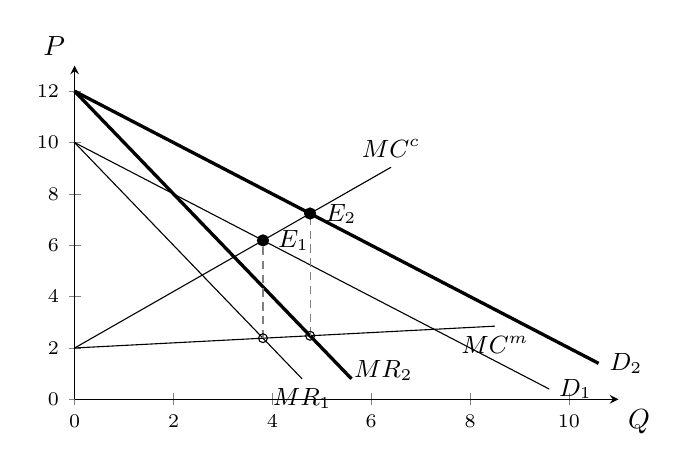
\begin{tikzpicture}
\begin{axis}[
  width=0.70\textwidth, height=0.48\textwidth,
  xmin=0, xmax=11, ymin=0, ymax=13,
  axis lines=left, xlabel={$Q$}, ylabel={$P$},
  xtick={0,2,4,6,8,10}, ytick={0,2,4,6,8,10,12},
  tick label style={font=\scriptsize},
  every axis x label/.style={at={(ticklabel* cs:1)}, anchor=north west},
  every axis y label/.style={at={(ticklabel* cs:1)}, anchor=south east},
  clip=false]
  \addplot[thin, domain=0:9.6, samples=2] {10 - x} node[pos=1, right, font=\small] {$D_1$};
  \addplot[very thick, domain=0:10.6, samples=2] {12 - x} node[pos=1, right, font=\small] {$D_2$};
  \addplot[thin, domain=0:4.6, samples=2] {10 - 2*x} node[pos=1, below, font=\small] {$MR_1$};
  \addplot[very thick, domain=0:5.6, samples=2] {12 - 2*x} node[pos=0.97, anchor=west, font=\small] {$MR_2$};
  \addplot[thin, domain=0:6.4, samples=2] {2 + 1.1*x} node[pos=1, above, font=\small] {$MC^c$};
  \addplot[thin, domain=0:8.5, samples=2] {2 + 0.1*x} node[pos=1, below, font=\small] {$MC^m$};
  \draw[densely dashed, gray] (axis cs:3.8095,2.381) -- (axis cs:3.8095,6.1905);
  \draw[densely dashed, gray] (axis cs:4.7619,2.476) -- (axis cs:4.7619,7.2381);
  \addplot[only marks, mark=*, mark size=2pt] coordinates {(3.8095,6.1905) (4.7619,7.2381)};
  \addplot[only marks, mark=o, mark size=1.6pt] coordinates {(3.8095,2.381) (4.7619,2.476)};
  \node[right, font=\small] at (axis cs:3.92,6.2) {$E_1$};
  \node[right, font=\small] at (axis cs:4.88,7.22) {$E_2$};
\end{axis}
\end{tikzpicture}
\caption[Observational equivalence under a parallel demand shift]{Observational equivalence under a parallel demand
shift. Demand shifts from $D_1\colon P = 10 - Q$ to $D_2\colon P = 12 - Q$. Competitive firms with $MC^c = 2 + 1.1Q$ and a
monopolist with $MC^m = 2 + 0.1Q$ both produce $E_1 = (3.81, 6.19)$ and $E_2 = (4.76, 7.24)$. Under monopoly, output is
set where $MR_i$ crosses $MC^m$ (open circles) and price is read off demand (dashed lines). Drawn after Figure~1 of
\citet{Bresnahan1982}, with illustrative numbers chosen here.}
\label{fig:03-bresnahan-shift}
\end{figure}

The two readings of the same data differ greatly in what they say about welfare. In the competitive reading the Lerner
index at $E_1$ is zero. In the monopoly reading marginal cost at $E_1$ is $2 + 0.1 \times 3.81 = 2.38$, so the Lerner
index is $\frac{6.19 - 2.38}{6.19} = 0.62$. The economics behind the equivalence is simple. When demand shifts out, price
rises in both models. Under competition it rises because marginal cost rises steeply with output. Under monopoly it rises
because marginal revenue shifts out while marginal cost barely moves. A parallel shift raises price either because
marginal cost rises with output or because of market power, and the ratio $\frac{\Delta P}{\Delta Q} = \lambda$ is the
same in both cases.

\subsection{Rotations of demand identify conduct}\label{sec:03-rotation}

\citet{Bresnahan1982} breaks the equivalence by letting an exogenous variable change the slope of demand. Let $Z_t$ be an
observed \emph{demand rotator}, and write demand as
\begin{equation}\label{eq:03-rotation-demand}
Q_t = a_0 + a_1 P_t + a_2 Y_t + a_3 P_t Z_t + a_4 Z_t + u^d_t ,
\end{equation}
with $a_1 + a_3 Z_t < 0$ on the support of $Z_t$. The slope of demand is $\frac{\partial Q_t}{\partial P_t} = a_1 + a_3 Z_t$,
which varies with $Z_t$ when $a_3 \neq 0$. We let $Z_t$ also shift the level of demand through $a_4$. Nothing below
requires $a_4 = 0$. Perceived marginal revenue is now $P_t + \theta\frac{Q_t}{a_1 + a_3 Z_t}$, and the supply relation
becomes
\begin{equation}\label{eq:03-rotation-supply}
P_t = b_0 + b_1 Q_t + \theta Q^*_t + b_2 W_t + u^s_t, \qquad
Q^*_t \equiv -\frac{Q_t}{a_1 + a_3 Z_t} = \frac{Q_t}{\lvert a_1 + a_3 Z_t\rvert} .
\end{equation}
The variable $Q^*_t$ is the \emph{markup term} $m_t \equiv \frac{Q_t}{\left\lvert \frac{\partial Q_t}{\partial P_t}\right\rvert} =
\frac{P_t}{\varepsilon_t}$. It is the dollar markup a monopolist would charge, so $\theta Q^*_t$ is the markup. With
$a_3 = 0$ the markup term is proportional to $Q_t$, and \eqref{eq:03-rotation-supply} collapses to the supply relation of
\eqref{eq:03-linear-system}. With $a_3 \neq 0$, the markup term moves with $Z_t$ at a given quantity, while the cost term
$b_1 Q_t$ does not.

\begin{proposition}[Rotations identify conduct]\label{prop:03-rotation}
Let demand be \eqref{eq:03-rotation-demand} with known parameters, and let the supply relation be
\eqref{eq:03-rotation-supply}. Let $X_t = (Y_t, Z_t, W_t)$, assume $\E[u^s_t \mid X_t] = 0$, and assume $Z_t$ does not
enter marginal cost. Suppose $\mu(X_t) \equiv \E[Q_t \mid X_t]$ is strictly monotone in $Y_t$ for each $(Z_t, W_t)$,
$a_3 \neq 0$, $Z_t$ takes at least two values, and $W_t$ is not degenerate. Then $(b_0, b_1, b_2, \theta)$ are identified.
\end{proposition}

\begin{proof}
Write $Q^*_t = g(Z_t)Q_t$ with $g(Z) \equiv -\frac{1}{a_1 + a_3 Z}$, a known function. Taking expectations of
\eqref{eq:03-rotation-supply} conditional on $X_t$ gives
\begin{equation*}
\E[P_t \mid X_t] = b_0 + b_1\, \mu(X_t) + \theta\, g(Z_t)\, \mu(X_t) + b_2 W_t .
\end{equation*}
The left side and $\mu(X_t)$ are features of the distribution of the data. Suppose a second vector $(b_0', b_1', b_2',
\theta')$ satisfies the same equation. Subtracting, the differences $c = (b_0 - b_0', b_1 - b_1', b_2 - b_2', \theta -
\theta')$ satisfy
\begin{equation*}
0 = c_0 + c_1\, \mu(X) + c_3\, g(Z)\, \mu(X) + c_2 W \quad \text{for all } X .
\end{equation*}
Fix $(Z, W)$ and vary $Y$. Since $\mu$ changes with $Y$, the coefficient on $\mu$ must vanish: $c_1 + c_3 g(Z) = 0$ for
every $Z$. Because $a_3 \neq 0$, the function $g$ takes different values at two values of $Z$, so $c_1 = c_3 = 0$. The
remaining condition $c_0 + c_2 W = 0$ for all $W$ gives $c_0 = c_2 = 0$.
\end{proof}

The proof has a transparent deterministic core. Suppose two markets share the same $W$ and the same quantity $Q$ but have
different rotators $Z_1 \neq Z_2$. The demand shifter $Y$ can always be chosen to make this happen. Marginal cost is then
the same in both markets, and the price difference isolates the markup:
\begin{equation*}
P_1 - P_2 = \theta\, Q\left[g(Z_1) - g(Z_2)\right] .
\end{equation*}
The bracket is nonzero when $a_3 \neq 0$, so the price difference reveals $\theta$. Once $\theta$ is known, two markets
with the same $Z$ and different $Q$ reveal $b_1$.

\casehead{Estimation}
The natural estimator has two steps. In the first step we estimate demand \eqref{eq:03-rotation-demand} by 2SLS. The
regressors $P_t$ and $P_tZ_t$ are endogenous, $(1, Y_t, Z_t)$ are included exogenous variables, and $W_t$ and $W_tZ_t$
are the excluded instruments. In the second step we construct
\begin{equation*}
\hat Q^*_t = -\frac{Q_t}{\hat a_1 + \hat a_3 Z_t}
\end{equation*}
and estimate the supply relation $P_t = b_0 + b_1 Q_t + \theta \hat Q^*_t + b_2 W_t + e_t$ by 2SLS. Here $Q_t$ and
$\hat Q^*_t$ are endogenous, $(1, W_t)$ are included exogenous variables, and $(Y_t, Z_t, Y_tZ_t)$ are the excluded
instruments. Three instruments for two endogenous regressors leave one overidentifying restriction to test. Because
$\hat Q^*_t$ is a generated regressor, conventional second-step standard errors are too small.
\citet[p.~1033, fn.~23]{Bresnahan1989} calls this explicit two-step procedure ``so ugly that no one would ever undertake
it'', while noting that it shows why more powerful techniques identify $\theta$.

The better procedure estimates both equations jointly by the generalized method of moments (GMM). Stack the parameters in
$\Theta = (a_0, \dots, a_4, b_0, b_1, b_2, \theta)$ and define the residuals
\begin{equation}\label{eq:03-rotation-gmm}
\begin{aligned}
u^d_t(\Theta) &= Q_t - a_0 - a_1 P_t - a_2 Y_t - a_3 P_t Z_t - a_4 Z_t ,\\
u^s_t(\Theta) &= P_t - b_0 - b_1 Q_t + \theta\, \frac{Q_t}{a_1 + a_3 Z_t} - b_2 W_t .
\end{aligned}
\end{equation}
With instrument vectors $h^d_t = (1, Y_t, Z_t, W_t, W_tZ_t)^\top$ and $h^s_t = (1, W_t, Y_t, Z_t, Y_tZ_t)^\top$, the
moment conditions are $\E[h^d_t u^d_t(\Theta)] = 0$ and $\E[h^s_t u^s_t(\Theta)] = 0$. GMM minimizes a quadratic form in the
sample analogues of the ten moments. The system is nonlinear in $\Theta$ because $\theta$ multiplies a ratio that involves
$(a_1, a_3)$. Joint estimation imposes the cross-equation restriction that the slope inside the markup term equals the
slope of demand, and its standard errors account for the estimation of demand automatically (\cref{app:econometrics}).

\casehead{A graphical version}
\Cref{fig:03-bresnahan-rotation} redraws Figure~2 of \citet{Bresnahan1982} in the same way. We keep $D_1$, $MC^c$, $MC^m$ and
$E_1 = (3.81, 6.19)$ from \cref{fig:03-bresnahan-shift}. Demand rotates around $E_1$ to the flatter curve
$D_3\colon P = 7.714 - 0.4Q$, which passes through $E_1$ because $6.19 + 0.4 \times 3.81 = 7.714$. The competitive
equilibrium solves $7.714 - 0.4Q = 2 + 1.1Q$, so $Q = \frac{5.714}{1.5} = 3.81$. Competition stays at $E_1$. The monopolist
sets $MR_3 = 7.714 - 0.8Q$ equal to $2 + 0.1Q$, so $Q = \frac{5.714}{0.9} = 6.35$ and $P = 7.714 - 0.4 \times 6.35 = 5.17$.
Monopoly moves to $E_3 = (6.35, 5.17)$. At $E_1$ the elasticity of demand rises from $\frac{6.19}{3.81} = 1.62$ to
$\frac{6.19}{0.4 \times 3.81} = 4.06$, and the monopolist cuts its markup.

\begin{figure}[htbp]
\centering
\begin{tikzpicture}
\begin{axis}[
  width=0.70\textwidth, height=0.45\textwidth,
  xmin=0, xmax=11, ymin=0, ymax=10.8,
  axis lines=left, xlabel={$Q$}, ylabel={$P$},
  xtick={0,2,4,6,8,10}, ytick={0,2,4,6,8,10},
  tick label style={font=\scriptsize},
  every axis x label/.style={at={(ticklabel* cs:1)}, anchor=north west},
  every axis y label/.style={at={(ticklabel* cs:1)}, anchor=south east},
  clip=false]
  \addplot[thin, domain=0:9.3, samples=2] {10 - x} node[pos=1, right, font=\small] {$D_1$};
  \addplot[thin, domain=0:4.6, samples=2] {10 - 2*x} node[pos=1, below, font=\small] {$MR_1$};
  \addplot[very thick, domain=0:10.6, samples=2] {7.7143 - 0.4*x} node[pos=1, right, font=\small] {$D_3$};
  \addplot[very thick, domain=0:8.6, samples=2] {7.7143 - 0.8*x} node[pos=1, below, font=\small] {$MR_3$};
  \addplot[thin, domain=0:6.4, samples=2] {2 + 1.1*x} node[pos=1, above, font=\small] {$MC^c$};
  \addplot[thin, domain=0:9.2, samples=2] {2 + 0.1*x} node[pos=1, right, font=\small] {$MC^m$};
  \draw[densely dashed, gray] (axis cs:6.3492,2.635) -- (axis cs:6.3492,5.1746);
  \addplot[only marks, mark=*, mark size=2.2pt] coordinates {(3.8095,6.1905)};
  \addplot[only marks, mark=*, mark size=1.6pt] coordinates {(6.3492,5.1746)};
  \addplot[only marks, mark=o, mark size=1.6pt] coordinates {(3.8095,2.381) (6.3492,2.635)};
  \node[font=\small] (e1lab) at (axis cs:3.2,7.7) {$E_1$};
  \draw[->, >=Stealth, thin] (e1lab.south east) -- (axis cs:3.74,6.33);
  \node[above right, font=\small] at (axis cs:6.35,5.25) {$E_3$};
\end{axis}
\end{tikzpicture}
\caption[A demand rotation separates competition from monopoly]{A demand rotation separates competition from monopoly.
Demand rotates around $E_1 = (3.81, 6.19)$ from $D_1\colon P = 10 - Q$ to $D_3\colon P = 7.714 - 0.4Q$. Competitive firms
with $MC^c = 2 + 1.1Q$ stay at $E_1$. A monopolist with $MC^m = 2 + 0.1Q$ sets $MR_3 = MC^m$ (open circle) and moves to
$E_3 = (6.35, 5.17)$. Drawn after Figure~2 of \citet{Bresnahan1982}, with illustrative numbers chosen here.}
\label{fig:03-bresnahan-rotation}
\end{figure}

The rotation does more than separate two polar models. The size of the response measures conduct. Write the magnitudes of
the inverse-demand slopes before and after the rotation as $g_1 = g(Z_1)$ and $g_3 = g(Z_3)$, with the function
$g(Z) = -\frac{1}{a_1 + a_3 Z} = \frac{1}{\lvert a_1 + a_3 Z\rvert}$ from the proof of \cref{prop:03-rotation}.
Every structure consistent with the original market has marginal cost slope $b_1(\theta) = \lambda_1 - \theta g_1$, where
$\lambda_1$ is the composite slope estimated before the rotation. After the rotation the supply relation has slope
$b_1(\theta) + \theta g_3 = \lambda_1 - \theta(g_1 - g_3)$. Since the original supply relation passed through $(Q_1, P_1)$,
the new one is
\begin{equation*}
P = P_1 + \left[\lambda_1 - \theta(g_1 - g_3)\right](Q - Q_1) - \theta(g_1 - g_3) Q_1 .
\end{equation*}
The rotated demand curve is $P = P_1 - g_3(Q - Q_1)$. Equating the two and solving,
\begin{align*}
(Q - Q_1)\left[g_3 + \lambda_1 - \theta(g_1 - g_3)\right] &= \theta(g_1 - g_3) Q_1 ,\\
Q_3 - Q_1 &= \frac{\theta(g_1 - g_3)Q_1}{g_3 + \lambda_1 - \theta(g_1 - g_3)} .
\end{align*}
Rearranging the first line at $Q = Q_3$ expresses conduct in terms of observables:
\begin{equation}\label{eq:03-rotation-response}
\theta = \frac{(g_3 + \lambda_1)(Q_3 - Q_1)}{(g_1 - g_3)\, Q_3} .
\end{equation}
In the example $g_1 = 1$, $g_3 = 0.4$ and $\lambda_1 = 1.1$. The response is zero under competition, $2.54$ under
monopoly, and $0.95$ when $\theta = 0.5$. Plugging the monopoly outcome into \eqref{eq:03-rotation-response} gives
$\frac{1.5 \times 2.54}{0.6 \times 6.35} = 1.00$. When demand becomes more elastic, a firm with market power cuts its
markup, and its output response rises with its conduct. At the original quantity the supply relation shifts down by
$\theta(g_1 - g_3)Q_1$, an amount proportional to conduct.

\casehead{Rotators in practice}
Applications need a natural experiment that changes the slope of demand \citep[pp.~1033--1034]{Bresnahan1989}. One
shifter might measure the size of the economy, such as national income, while a second measures the price of a
substitute. In \citet{JustChern1980} the market power lies on the buying side. Tomato processors buy from many farmers,
and the adoption of a mechanical harvester changed the elasticity of supply they faced. In
\citet{Bresnahan1981,Bresnahan1987} demand elasticities depend on how crowded the product space is, which changes with
the set of models offered (\cref{ch:discrete}). In sugar refining the canning season changes the composition of buyers
and makes demand less elastic (\cref{sec:03-sugar}). The method stands or falls with the estimated demand elasticities.
Critics offered other readings of the tomato harvester, and the automobile results depend on how products are ordered in
quality space \citep[p.~1034]{Bresnahan1989}.

Two caveats follow from the theory. First, the rotator must be excluded from marginal cost. If the canning season also
changes the slope of marginal cost, through overtime for example, then a term $b_3 Z_t Q_t$ in marginal cost competes with
$\theta g(Z_t) Q_t$. The two differ only through the curvature of $g$, a thin reed for identification. Second, the
linear model can identify $\theta$ even without a separate shifter $Y_t$, using $Z_t$ and $Z_t^2$ as instruments. That
identification comes entirely from the linearity of marginal cost in quantity, as the next theorem shows.

\subsection{Lau's theorem: identification without functional forms}\label{sec:03-lau}

The rotation argument does not depend on linearity. \citet{Lau1982} shows that it holds for general demand and cost
functions. \citet[p.~1033]{Bresnahan1989} summarizes his sufficient condition for identification. The inverse demand
function must not be writable with the demand shifters separable from quantity, which requires at least two shifters.
We state and prove a version of this result.

Let inverse demand be $P = f(Q, Y)$ with a vector of demand shifters $Y \in \R^k$ and $f_Q < 0$, and let industry
marginal cost be an unknown function $c(Q, W)$. The supply relation is
\begin{equation}\label{eq:03-lau-model}
P = c(Q, W) - \theta\, Q\, f_Q(Q, Y) .
\end{equation}
Following Lau, we work without econometric errors. The data are the equilibrium map $(Y, W) \mapsto (P, Q)$.
\citet[p.~1776]{BerryHaile2014} describe the class Lau studied as deterministic conjectural-variations models with
homogeneous goods and symmetric firms. We make three assumptions. The demand function $f$ is known, because the cost
shifters $W$ are excluded from demand and trace it out. Each structure considered has a unique equilibrium with $Q > 0$
for every $(Y, W)$. The function $f$ is twice continuously differentiable.

\begin{definition}[Single-index demand]\label{def:03-single-index}
Inverse demand has a \emph{single index} if $f(Q, Y) = \tilde g(Q, r(Y))$ for a scalar function $r$ and some
function $\tilde g$.
\end{definition}

\begin{theorem}[Lau]\label{prop:03-lau}
\leavevmode
\begin{enumerate}[label=(\roman*)]
\item Suppose demand has a single index, and for each $W$ the equilibrium quantity $Q^e(r, W)$ is strictly monotone in
  the index $r$. Then for every $\theta' \ge 0$ there is a marginal cost function $c'(Q, W)$ such that the structure
  $(f, c', \theta')$ reproduces every observed equilibrium. Conduct is not identified.
\item Suppose that at some observed equilibrium $(Q_0, Y_0, W_0)$ the $2 \times k$ Jacobian of
  $\left(f(Q_0, Y), f_Q(Q_0, Y)\right)$ with respect to $Y$ has rank two at $Y_0$. Suppose also that the equilibrium
  map is observed for all $Y$ in a neighborhood of $Y_0$ with $W = W_0$. Then $\theta$ is identified.
\end{enumerate}
\end{theorem}

\begin{proof}
(i) Fix $W$. Because $Q^e(\cdot, W)$ is strictly monotone, it has an inverse $r = H(Q, W)$ on its range. Define
\begin{equation*}
c'(Q, W) \equiv \tilde g\left(Q, H(Q, W)\right) + \theta'\, Q\, \tilde g_Q\left(Q, H(Q, W)\right) ,
\end{equation*}
which depends on $(Q, W)$ only. Take any observed equilibrium $(P, Q)$ at $(Y, W)$ and let $r = r(Y)$. Then
$Q = Q^e(r, W)$, so $H(Q, W) = r$ and $P = \tilde g(Q, r)$. Substituting,
\begin{equation*}
c'(Q, W) = P + \theta'\, Q\, \tilde g_Q(Q, r) = P + \theta'\, Q\, f_Q(Q, Y) .
\end{equation*}
Rearranging gives $P = c'(Q, W) - \theta' Q f_Q(Q, Y)$, which is the supply relation of the alternative structure. Demand
is unchanged. The observed point is therefore an equilibrium of $(f, c', \theta')$, and by uniqueness it is the only one.

(ii) Fix $W_0$ and define $\Phi(Q, Y) \equiv f(Q, Y) + \theta Q f_Q(Q, Y) - c(Q, W_0)$, so equilibria satisfy
$\Phi = 0$. Consider the set $\Gamma = \{Y : \Phi(Q_0, Y) = 0\}$ of shifter values that produce the equilibrium quantity
$Q_0$. Its gradient at $Y_0$ is $\nabla f + \theta Q_0 \nabla f_Q$, where gradients are taken with respect to $Y$. This
gradient is nonzero, because $\nabla f$ and $\nabla f_Q$ are linearly independent. By the implicit function theorem,
$\Gamma$ is locally a manifold of dimension $k - 1$ through $Y_0$, with tangent space
$T = \{v : (\nabla f + \theta Q_0 \nabla f_Q)\cdot v = 0\}$. Suppose $f_Q(Q_0, \cdot)$ were constant on $\Gamma$ near
$Y_0$. Then $\nabla f_Q \cdot v = 0$ for all $v \in T$, so $\nabla f_Q = \ell(\nabla f + \theta Q_0\nabla f_Q)$ for some
scalar $\ell$. If $\ell \ne 0$, this makes $\nabla f$ and $\nabla f_Q$ linearly dependent. If $\ell = 0$, it makes
$\nabla f_Q = 0$. Both contradict rank two. Hence some $Y_1 \in \Gamma$ has $f_Q(Q_0, Y_1) \neq f_Q(Q_0, Y_0)$. The two
equilibria share $Q_0$ and $W_0$, hence the same marginal cost $c(Q_0, W_0)$. Subtracting their supply relations,
\begin{equation}\label{eq:03-lau-theta}
P_1 - P_0 = -\theta\, Q_0 \left[f_Q(Q_0, Y_1) - f_Q(Q_0, Y_0)\right], \qquad
\theta = -\frac{P_1 - P_0}{Q_0\left[f_Q(Q_0, Y_1) - f_Q(Q_0, Y_0)\right]} .
\end{equation}
Every term on the right is observed or known, so $\theta$ is identified.
\end{proof}

The two parts fit together. Under a single index, $f$ and $f_Q$ depend on $Y$ only through $r$. Their Jacobian is
$\left(\tilde g_r \nabla r, \tilde g_{Qr}\nabla r\right)$, which has rank at most one. Part (ii) is therefore the local
failure of the single-index structure. In words, $\theta$ is identified when the demand shifters can move the slope of
demand at a given quantity independently of its level. In the data, every observation with the same $W$ lies on a single
curve $P = \phi(Q, W)$ when demand has a single index. Any conduct value can then be rationalized by a suitable marginal
cost, as part (i) constructs.

Three examples make the condition concrete. Constant-elasticity demand with a scale shifter, $Q = Y P^{-\varepsilon}$, has
inverse demand $P = (\frac{Q}{Y})^{-\frac{1}{\varepsilon}}$, a single index. Conduct is not identified without restrictions
on cost. Letting a second shifter move the elasticity, $Q = Y_1 P^{-\varepsilon(Y_2)}$, breaks the single index. In the
linear rotation model \eqref{eq:03-rotation-demand}, inverse demand is $f = \frac{Q - a_0 - a_2 Y - a_4 Z}{a_1 + a_3 Z}$ with
$f_Q = \frac{1}{a_1 + a_3 Z}$. The Jacobian with respect to $(Y, Z)$ has determinant
\begin{equation*}
\frac{\partial f}{\partial Y}\frac{\partial f_Q}{\partial Z} - \frac{\partial f}{\partial Z}\frac{\partial f_Q}{\partial Y}
= \left(-\frac{a_2}{a_1 + a_3 Z}\right)\left(-\frac{a_3}{(a_1 + a_3 Z)^2}\right) - 0
= \frac{a_2 a_3}{(a_1 + a_3 Z)^3} ,
\end{equation*}
which is nonzero exactly when both $a_2 \neq 0$ and $a_3 \neq 0$. A pure rotator without a shifter ($a_2 = 0$) leaves a
single index $r = Z$, so the identification in the linear model with $a_2 = 0$ rests on the functional form of cost. This
matches an observation of \citet[p.~1754]{BerryHaile2014}. Lau's results require exogenous variation that alters both
the level and the slope of aggregate demand, a point they credit to \citet{Nevo1998}. Nothing in the proof uses
linearity, which is the sense in which the rotation argument is nonparametric.

\subsection{Other routes to identification}\label{sec:03-other-routes}

Demand rotations are one of several ways to separate conduct from the slope of marginal cost. Each replaces the rotator
with a restriction or with extra data, and each restriction has a cost.

Constant marginal cost makes a single demand shifter enough. With $b_1 = 0$ the composite slope is $\lambda =
-\frac{\theta}{a_1}$, so $\theta = -a_1\lambda$, the upper endpoint in \cref{cor:03-obs-equiv-bounds}. Equivalently,
pass-through reveals conduct. With linear demand and constant marginal cost, $\rho = \frac{1}{1 + \theta}$ by
\cref{cor:03-passthrough-cases}(iii), which is the logic of the pass-through tests of \cref{sec:03-passthrough-theory}.
The weakness is that any slope of marginal cost is read as market power, so the method overstates $\theta$ when
$b_1 > 0$.

Observed marginal cost removes the problem. Once demand is estimated, $\theta_t = \varepsilon_t L_t$ can be computed
observation by observation from \eqref{eq:03-lerner-theta}. This is the strategy of the two validation studies of this
chapter. In British electricity, marginal cost comes from fuel prices and plant efficiencies (\cref{sec:03-electricity}).
In insurance markets, claims data can play the same role, because the cost of serving a customer is the expected claim.
A related route assumes that cost is known up to a few parameters. In sugar refining the fixed-proportions technology
gives $MC = c_0 + kP^{raw}$, and $c_0$ and $k$ can be estimated jointly with $\theta$ or set from engineering evidence
(\cref{sec:03-sugar}).

Homogeneity of marginal cost in factor prices gives another restriction. Any term of the supply relation that does not
scale with factor prices must belong to the markup, the route of \citet{Appelbaum1982} described in
\cref{sec:03-taxonomy}. Firm-specific cost shifters identify a single firm's residual demand, an object different from
industry conduct (\cref{sec:03-residual-demand}).

Changes in market structure or regulation can shift conduct while leaving cost unchanged. \citet{SpillerFavaro1984} study
Uruguayan banking across a change in the regulation of entry. They find that freer entry shifts the supply relation
downward \citep[fn.~36]{Bresnahan1989}. The identifying assumption is that the regulatory change moved conduct and left
marginal cost alone.

Supply shocks identify regimes of conduct. \citet{Porter1983} lets the supply relation switch between a price-war regime
with low conduct and a collusive regime with high conduct. \citet[Section~3.4]{Bresnahan1989} explains what identifies the
switch. Holding the exogenous variables fixed, the joint distribution of price and quantity has two modes, one per regime,
and switching-regression methods detect them. The risk is that an unobserved cost shock also shifts the supply relation.
In the railroad data the regime changes move price and quantity by about 50 percent, which, together with contemporary
discussion of cartel adherence, makes the conduct reading plausible \citep[p.~1042]{Bresnahan1989}. We study this work in
\cref{ch:collusion-evidence}.

The modern literature recasts identification of conduct as testing among a finite menu of models, such as Bertrand pricing,
joint profit maximization or pricing that internalizes common ownership. \citet{Bresnahan1987} compares collusive and
competitive models of the 1955 automobile market (\cref{ch:discrete}). \citet{Nevo2001} compares the margins implied by
alternative conduct models with accounting margins in breakfast cereal (\cref{ch:blp}). \citet[Section~6]{BerryHaile2014}
give nonparametric conditions under which cross-market and cross-product variation discriminates between conduct models.
Their argument generalizes the rotation logic beyond rotations. \citet{BackusConlonSinkinson2021} and
\citet{DuarteEtAl2024} turn it into practical tests built on the model-selection test of \citet{RiversVuong2002}. Their
instruments must move markups but be excluded from marginal cost. \citet[Section~2.2]{BackusConlonSinkinson2021} show
that the test gains power when the instrument predicts the difference between the markups of the two models.
\citet[Section~5]{DuarteEtAl2024} show that weak instruments distort the size and lower the power of the test, and they
give a diagnostic for instrument strength.

\section{Interpreting the conduct parameter}\label{sec:03-interpreting}

Suppose the identification problem is solved and we have an estimate $\hat\theta$ strictly between zero and one. What
have we learned? This section asks where the conduct parameter comes from. It shows that a constant-$\theta$ estimate
can mismeasure market power badly when conduct varies, presents a bounds alternative, and reviews the record of estimates.

\subsection{Where the conduct parameter comes from}\label{sec:03-theta-origins}

The literature reads $\theta$ in three ways. The first treats it as shorthand for a specific game. Homogeneous-good
Bertrand pricing gives $\theta = 0$, symmetric Cournot gives $\theta = \frac{1}{N}$, and joint profit maximization gives
$\theta = 1$ (\cref{ch:theory}). Dynamic games can make conduct vary over time. In \citet{GreenPorter1984}, firms cannot
observe demand shocks or rivals' outputs, low prices trigger reversion to a punishment phase, and conduct alternates
between collusion and price wars (\cref{ch:collusion-theory}). Studies in this tradition impose a lot of structure on
$\theta$ in the econometric specification.

The second reading treats $\theta$ as a continuous \emph{conjectural variation}, the firm-level parameter
$\tilde\theta_i = 1 + r_i$ of \cref{cor:03-benchmarks}. Conjectures of this kind go back to \citet{Bowley1924}. Three
criticisms followed. The first is that the approach lacks a consistent theory. In a static game firms move
simultaneously, so a nonzero response has no foundation. The attempt to discipline conjectures by requiring them to be
consistent ended with \citet{Daughety1985} and \citet{Lindh1992}. Without peculiar informational assumptions, Cournot
conjectures are the only consistent ones \citep[p.~230]{Corts1999}. The second is that the
parameter is hard to interpret as a belief. As \cref{rem:03-cv-language} explains, it describes what firms do and says
nothing about what they expect rivals to do. The third is the identification problem of \cref{sec:03-identification}.

The third reading uses $\hat\theta$ only as a specification test. We estimate $\theta$ freely and test $\theta = 0$,
$\theta = \frac{1}{N}$ or $\theta = 1$ without giving $\hat\theta$ a structural meaning. Every specification nests price
taking, so every estimate tests it (\cref{sec:01-appelbaum}).

Two normalizations coexist, and we must keep them apart. Corts writes a firm-level supply relation in which conduct equals
0 under competition, 1 under Cournot and $N$ under joint monopoly. When all firms share the same conduct, the industry
parameter of \eqref{eq:03-supply-relation} is the firm-level parameter divided by $N$ \citep[fn.~1]{Corts1999}. We use the
industry normalization throughout and say so whenever we quote a firm-level number.

The \emph{as-if} reading interprets an estimate in $(0, 1)$ through \eqref{eq:03-lerner-theta}. Whatever game firms play,
we can compute the conduct value that would rationalize the observed margin, $\theta_t = \varepsilon_t L_t$, the
\emph{elasticity-adjusted Lerner index}. It separates industries with high margins because demand is inelastic from
industries with high margins because conduct is less competitive \citep[p.~231]{Corts1999}. \citet[p.~1029]{Bresnahan1989}
states the conditions for this reading. If the estimated ``conjectures'' are constant over time and breakdowns of collusion
are infrequent, ``we can safely interpret the parameters as measuring the average collusiveness of conduct.'' The exact-fit
result of \cref{prop:03-exact-fit} shows why some such condition is needed. A conduct parameter free to vary by observation
fits any data, and a constant $\theta$ is the restriction that gives the model content. What does a constant-$\theta$
estimate measure when conduct does vary? That is the question of \citet{Corts1999}.

\subsection{The Corts critique}\label{sec:03-corts}

\subsubsection{The question}

\citet{Corts1999} asks whether what he calls the \emph{conduct parameter method} recovers the as-if conduct parameter when
behavior is generated by a game other than a conjectural-variations equilibrium. The question matters because the method
was popular when Corts wrote, and it remains in use. Its data requirements are modest and its output is a single, easily interpreted number. Corts
lists more than a dozen applications, among them \citet{Iwata1974}, \citet{Appelbaum1982}, \citet{Porter1983},
\citet{Roberts1984}, \citet{SpillerFavaro1984} and \citet{Ellison1994}.

Corts separates the method into two steps \citep[p.~229]{Corts1999}. The first estimates the slope of the supply
relation, which he calls \emph{equilibrium variation}: how equilibrium behavior responds to perturbations of demand. The
second maps this slope into the \emph{equilibrium value} of the elasticity-adjusted margin. The literature has handled the
first step with care, through constant marginal cost \citep{Iwata1974}, demand rotators \citep{Bresnahan1982,Lau1982}, or
supply shocks and regimes \citep{Porter1983}. Corts attacks the second step. He makes the first step trivial by assuming
constant marginal cost, linear demand and a symmetric equilibrium.

\subsubsection{What the conduct parameter method estimates}

We first state the result in a general form. Let the true markup satisfy
\begin{equation}\label{eq:03-corts-markup}
P_t = c_0 + c_W^\top W_t + \theta_t m_t, \qquad m_t \equiv \frac{Q_t}{\left\lvert \frac{\partial Q_t}{\partial P_t}\right\rvert} =
\frac{P_t}{\varepsilon_t},
\end{equation}
so that $\theta_t = \varepsilon_t L_t$ is the as-if conduct in market $t$. Marginal cost $c_0 + c_W^\top W_t$ is
constant in output, its level is unknown, and it shifts with observed cost shifters $W_t$. Demand is known, so $m_t$ is
observed. This is the most favorable case for the method. If marginal cost were known, $\theta_t$ could be computed
directly and nothing would need to be estimated. The researcher assumes constant conduct and estimates
$P_t = c_0 + c_W^\top W_t + \theta m_t + v_t$ by instrumental variables, using a demand shifter or rotator $Z_t$ as the
instrument for $m_t$.

\begin{proposition}[What a constant conduct parameter estimates]\label{prop:03-corts}
Let $\tilde Z_t$ be the residual from the linear projection of $Z_t$ on $(1, W_t)$, and assume $\Cov(\tilde Z_t, m_t) \neq 0$.
\begin{enumerate}[label=(\roman*)]
\item The instrumental-variables estimator converges to
  \begin{equation}\label{eq:03-corts-estimand}
  \plim \hat\theta = \frac{\Cov(\tilde Z_t, \theta_t m_t)}{\Cov(\tilde Z_t, m_t)}
  = \E[\theta_t] + \frac{\Cov\left(\tilde Z_t, (\theta_t - \E[\theta_t])\, m_t\right)}{\Cov(\tilde Z_t, m_t)} .
  \end{equation}
  It equals average conduct if conduct is constant, or if $\theta_t$ is independent of $(Z_t, W_t, m_t)$. In general the
  second term is not zero and can have either sign.
\item Suppose there are no cost shifters, $Z_t$ is continuous with support bounded below, $m_t = \mu(Z_t)$ for a
  differentiable increasing function $\mu$, and the markup is a differentiable function of the markup term,
  $\theta_t m_t = \mathcal{M}(m_t)$. Then
  \begin{equation*}
  \plim \hat\theta = \int \mathcal{M}'\left(\mu(z)\right) \omega(z)\, \dd z, \qquad
  \omega(z) = \frac{\mu'(z)\, \upsilon(z)}{\int \mu'(s)\, \upsilon(s)\, \dd s} \ge 0,
  \end{equation*}
  where $\upsilon(z) = \E\left[(Z_t - \E Z_t)\indic\{Z_t \ge z\}\right]$.
  The estimate is a weighted average of the local slopes $\mathcal{M}'$ of the supply relation.
\end{enumerate}
\end{proposition}

\begin{proof}
(i) By the Frisch-Waugh logic for instrumental variables, the coefficient on $m_t$ in a just-identified regression with
exogenous controls $(1, W_t)$ is $\frac{\Cov(\tilde Z_t, P_t)}{\Cov(\tilde Z_t, m_t)}$ in the limit. Substitute
\eqref{eq:03-corts-markup} for $P_t$. The term $c_0 + c_W^\top W_t$ is a linear function of $(1, W_t)$, so its
covariance with $\tilde Z_t$ is zero, which leaves the first expression. For the second, write $\theta_t m_t =
\E[\theta_t] m_t + (\theta_t - \E[\theta_t]) m_t$ and divide. If $\theta_t$ is independent of $(Z_t, W_t, m_t)$, then
$\Cov(\tilde Z_t, (\theta_t - \E\theta_t)m_t) = \E[\theta_t - \E\theta_t]\,\E[\tilde Z_t m_t] = 0$, because $\tilde Z_t$ is
a function of $(Z_t, W_t)$ and has mean zero.

(ii) Let $\underline z$ be the lower end of the support. For any differentiable $h$, $h(Z) = h(\underline z) +
\int \indic\{Z \ge z\} h'(z)\, \dd z$, so $\Cov(Z, h(Z)) = \int h'(z)\,\Cov(Z, \indic\{Z \ge z\})\, \dd z = \int h'(z)\upsilon(z)\,
\dd z$. The weight $\upsilon(z)$ is nonnegative. For $z \ge \E Z$ it is the expectation of a nonnegative variable. For
$z < \E Z$ it equals $-\E[(Z - \E Z)\indic\{Z < z\}]$, minus the expectation of a nonpositive variable. Apply the identity
to $h = \mathcal{M} \circ \mu$, with $h' = \mathcal{M}'(\mu)\mu'$, and to $h = \mu$, then take the ratio.
\end{proof}

Part (ii) connects the critique to the interpretation of instrumental variables in simultaneous equations as weighted
averages of derivatives, a link Corts draws in his footnote 5. He cites the 1995 NBER working paper that later appeared as
\citet{AngristGraddyImbens2000}. The level of conduct at
markup term $m$ is $\frac{\mathcal{M}(m)}{m}$, the slope of the ray from the origin. The estimate averages the slope of the
supply relation itself. A small-dispersion version makes the gap explicit. If $\theta_t = \theta(m_t)$ and $m_t$ varies
little around $\bar m$, then $\mathcal{M}(m) \approx \mathcal{M}(\bar m) + \mathcal{M}'(\bar m)(m - \bar m)$ and
\begin{equation}\label{eq:03-corts-local}
\plim \hat\theta \approx \mathcal{M}'(\bar m) = \theta(\bar m) + \bar m\, \theta'(\bar m)
= \theta(\bar m)\left(1 + \eta_\theta\right), \qquad \eta_\theta \equiv \frac{\dd\ln\theta}{\dd\ln m} .
\end{equation}
The estimate equals the level of conduct only when conduct does not vary with demand conditions. If collusion weakens when
demand is high ($\eta_\theta < 0$), the estimate understates conduct. If $\eta_\theta < -1$, it is negative.

\begin{example}[Conduct linear in the markup term]\label{ex:03-corts-linear}
Let $\theta_t = \vartheta_0 - \vartheta_1 m_t$ with $\vartheta_1 > 0$, so collusion is harder when demand is strong, as in
\citet{RotembergSaloner1986}. Then $\theta_t m_t = \vartheta_0 m_t - \vartheta_1 m_t^2$. With no cost shifters, and
writing $m_t = \bar m + d_t$ with $\bar m = \E[m_t]$,
\begin{equation*}
\Cov(Z_t, m_t^2) = 2\bar m\, \Cov(Z_t, m_t) + \E\left[(Z_t - \E Z_t)\, d_t^2\right] .
\end{equation*}
If $(Z_t, m_t)$ is jointly symmetric about its mean, the last term is zero, and \eqref{eq:03-corts-estimand} gives
\begin{equation*}
\plim\hat\theta = \vartheta_0 - \vartheta_1\frac{\Cov(Z_t, m_t^2)}{\Cov(Z_t, m_t)} = \vartheta_0 - 2\vartheta_1\bar m ,
\qquad \E[\theta_t] = \vartheta_0 - \vartheta_1\bar m .
\end{equation*}
The estimate understates average conduct by $\vartheta_1\bar m$, and it is negative whenever $\vartheta_0 < 2\vartheta_1\bar
m$. With $\vartheta_0 = 1$ and $\vartheta_1\bar m = 0.6$, average conduct is $0.4$ while the estimate is $-0.2$.
\end{example}

Corts derives the special case of linear demand. Let inverse demand be $P_t = A(x_t) - BQ_t + e_t$, where $A(x) = A_0 +
A_1 x$ with $A_1 > 0$ and $x_t$ is a demand shifter, and let marginal cost be constant in output. Each of $N$ symmetric
firms produces $q_t = \frac{Q_t}{N}$. The firm-level supply relation is $P_t = c(w_t) + \theta_i B q_t$. Two-stage least
squares with instrument $x_t$ gives a coefficient on $q_t$ equal to $\frac{A_1}{\gamma_q} - NB$ in the limit
\citep[eqs.~7--8]{Corts1999}. Here $\gamma_q$ is the first-stage coefficient of $q_t$ on $x_t$ after partialling out
$w_t$. The
firm-level conduct estimate is this coefficient divided by $B$:
\begin{equation*}
\plim\hat\theta_i = \frac{A_1}{B\gamma_q} - N \qquad \text{\citep[eq.~9]{Corts1999}}.
\end{equation*}
It depends only on demand parameters and on how equilibrium quantity responds to the demand shifter. When the optimal
quantity rule $q^*(x)$ is linear, $\gamma_q = \frac{\dd q^*}{\dd x}$ and the estimate is the slope of the margin with respect to
demand-driven quantity, $\hat\theta_i = \frac{1}{B}\left(\frac{\dd(P - c)}{\dd x}\right)\left(\frac{\dd q^*}{\dd x}\right)^{-1}$ \citep[eq.~10]{Corts1999}. The as-if
parameter is $\tilde\theta_i = \frac{P - c}{Bq^*}$. Corts's Proposition~1 follows. The method measures market power
correctly if and only if
\begin{equation*}
\frac{P - c}{q^*} = \left(\frac{\dd(P - c)}{\dd x}\right)\left(\frac{\dd q^*}{\dd x}\right)^{-1} ,
\end{equation*}
that is, if and only if the average relation between margin and output equals the marginal relation.

\Cref{fig:03-corts-slope} illustrates the point in the spirit of Corts's Figure~1. In a conjectural-variations model the
supply relation is a ray from the marginal cost intercept, so its slope and its level coincide. Another game can generate
a flatter supply relation through points with the same average markup. The method then infers lower conduct and assigns
the rest of the margin to a higher marginal cost intercept.

\begin{figure}[htbp]
\centering
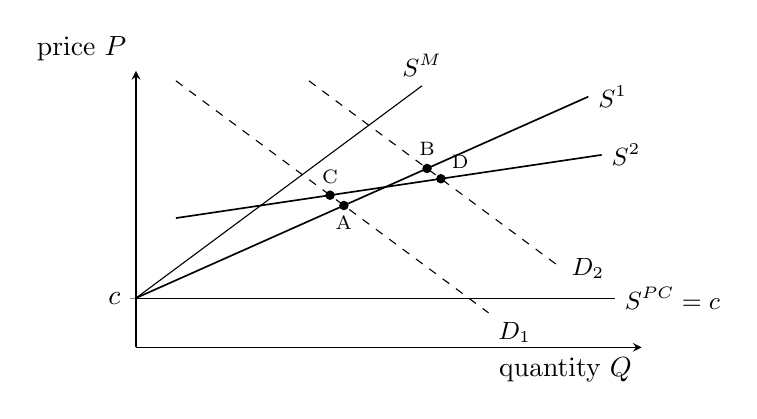
\begin{tikzpicture}
\begin{axis}[
  width=0.66\textwidth, height=0.42\textwidth,
  xmin=0, xmax=7.6, ymin=0, ymax=5.6,
  axis lines=left, xlabel={quantity $Q$}, ylabel={price $P$},
  xtick=\empty, ytick={1}, yticklabels={$c$},
  every axis x label/.style={at={(ticklabel* cs:1)}, anchor=north east},
  every axis y label/.style={at={(ticklabel* cs:1)}, anchor=south east},
  clip=false]
  \addplot[thin, domain=0:7.2, samples=2] {1} node[pos=1, right, font=\small] {$S^{PC} = c$};
  \addplot[thin, domain=0:4.3, samples=2] {1 + x} node[pos=1, above, font=\small] {$S^{M}$};
  \addplot[semithick, domain=0:6.8, samples=2] {1 + 0.6*x} node[pos=1, right, font=\small] {$S^{1}$};
  \addplot[semithick, domain=0.6:7.0, samples=2] {2.5 + 0.2*x} node[pos=1, right, font=\small] {$S^{2}$};
  \addplot[dashed, domain=0.6:5.3, samples=2] {6 - x} node[pos=1, below right, font=\small] {$D_1$};
  \addplot[dashed, domain=2.6:6.4, samples=2] {8 - x} node[pos=1, right, font=\small] {$D_2$};
  \addplot[only marks, mark=*, mark size=1.5pt] coordinates {(3.125,2.875) (4.375,3.625) (2.9167,3.0833) (4.5833,3.4167)};
  \node[below, font=\scriptsize] at (axis cs:3.125,2.85) {A};
  \node[above, font=\scriptsize] at (axis cs:4.375,3.68) {B};
  \node[above, font=\scriptsize] at (axis cs:2.9167,3.12) {C};
  \node[above right, font=\scriptsize] at (axis cs:4.6,3.42) {D};
\end{axis}
\end{tikzpicture}
\caption[Slope versus level of the supply relation]{Slope versus level of the supply relation. Inverse demand shifts from
$D_1\colon P = 6 - Q$ to $D_2\colon P = 8 - Q$, and marginal cost is $c = 1$. Industry 1 follows the conjectural-variations
supply relation $S^1\colon P = 1 + 0.6Q$ (points A and B). Industry 2 follows $S^2\colon P = 2.5 + 0.2Q$ (points C and D).
Both industries have average markup $2.25$ at average quantity $3.75$, an $m$-weighted average conduct of $0.6$. The conduct parameter
method estimates $0.6$ for industry 1 and $0.2$ for industry 2, and attributes the rest of industry 2's margin to a
marginal cost of $2.5$. $S^{PC}$ and $S^M$ are the competitive and monopoly supply relations. Drawn in the spirit of
Figure~1 of \citet{Corts1999}.}
\label{fig:03-corts-slope}
\end{figure}

The numbers in \cref{fig:03-corts-slope} are easy to check. On $S^1$, point A solves $6 - Q = 1 + 0.6Q$, so $Q = 3.125$
and the markup is $1.875$. Point B solves $8 - Q = 1 + 0.6Q$, so $Q = 4.375$ and the markup is $2.625$. On $S^2$, point C
solves $6 - Q = 2.5 + 0.2Q$, so $Q = 2.917$ and the markup is $2.083$. Point D gives $Q = 4.583$ and markup $2.417$. Both
pairs average a markup of $2.25$ at quantity $3.75$. The ratio $\frac{2.25}{3.75} = 0.6$ is the $m$-weighted average
conduct $\frac{\E[\theta_t m_t]}{\E[m_t]}$, since $m_t = Q_t$ when the slope of demand is $-1$.

\subsubsection{Corts's supergame model}

To show that the gap can be large in a coherent model, Corts studies efficient tacit collusion supported by repeated
interaction \citep[Section~3]{Corts1999}. The model is closely related to \citet{RotembergSaloner1986} when demand is
independent over time and to \citet{Kandori1991} when it is serially correlated \citep[fn.~2]{Corts1999}. We use
$\delta$ for the discount factor in the rest of this subsection. $N$
symmetric firms choose quantities every period. Inverse demand is $P_t = A(x_t) - BQ_t$ and marginal cost is $c(w_t)$,
where the demand state $x_t$ and the cost state $w_t$ are observed by all firms before they choose. A deviation is
punished by reversion to the one-shot Cournot equilibrium forever. An \emph{efficient} supergame equilibrium chooses, in
each state, the quantity that maximizes joint profit subject to the incentive constraint. Let $y_t = A(x_t) - c(w_t)$ be
the demand margin and $q$ the output of each firm.

The incentive constraint takes a simple form. A firm's collusive profit is $\pi(q) = q(y_t - BNq)$. Against rivals who
produce $(N - 1)q$, the best deviation produces $\frac{y_t - B(N - 1)q}{2B}$ and earns $\pi^b(q) = \frac{(y_t - B(N -
1)q)^2}{4B}$. The one-period gain from deviating is
\begin{align*}
\pi^b(q) - \pi(q) &= \frac{(y_t - B(N - 1)q)^2 - 4Bq(y_t - BNq)}{4B}\\
&= \frac{y_t^2 - 2B(N + 1)\, q\, y_t + B^2\left[(N - 1)^2 + 4N\right]q^2}{4B}\\
&= \frac{\left(y_t - B(N + 1)q\right)^2}{4B} .
\end{align*}
Let $\Lambda(x_t)$ be the expected discounted profit lost by entering the punishment phase \citep[eq.~15]{Corts1999}. It sums,
over future periods $i \ge 1$, $\delta^i$ times the expected excess of collusive over Cournot profit. The incentive
constraint is $\frac{(y_t - B(N + 1)q)^2}{4B} \le \Lambda(x_t)$. Collusive output lies below the Cournot output $q^c =
\frac{y_t}{B(N + 1)}$, so the constraint reads $y_t - B(N + 1)q \le 2\sqrt{B \Lambda(x_t)}$. The smallest sustainable output is
\begin{equation}\label{eq:03-corts-qtilde}
\tilde q_t = \frac{y_t}{B(N + 1)} - \frac{2\sqrt{B \Lambda(x_t)}}{B(N + 1)} \qquad \text{\citep[eq.~14]{Corts1999}}.
\end{equation}
The efficient output is the joint-monopoly output $q^m_t = \frac{y_t}{2BN}$ when it is sustainable, and $\tilde q_t$
otherwise. In industry units, conduct in state $t$ is $\theta_t = \frac{P_t - c_t}{BQ_t}$, which equals 1 at $q^m_t$ and
$\frac{1}{N}$ at $q^c$.

Equation \eqref{eq:03-corts-qtilde} shows why persistence matters. A higher demand state raises the gain from deviating,
which pushes output up toward Cournot. If demand is persistent, a higher state also raises expected future collusive
profits and so the cost of punishment $\Lambda(x_t)$, which pushes output down. When shocks are independent over time, only the
first effect operates. Then $\Lambda$ does not depend on $x_t$, and $\frac{\dd\tilde q_t}{\dd x_t} = \frac{A_1}{B(N + 1)}$, the
Cournot response.

\casehead{Simulation design and results}
Corts simulates a symmetric duopoly with linear demand and constant marginal cost. The demand and cost states each take
ten evenly spaced values. The cost state is independent over time, and its role is to identify demand. The demand state
follows a Markov chain that stays in the same state with probability $\varpi$ and moves to each other state with
probability $\frac{1 - \varpi}{9}$ (Corts calls this probability $\lambda$). Firms' quantities are computed by iterating
on $\Lambda(x_t)$ until convergence, and the conduct parameter method is applied to a sample from the resulting process.

\Cref{fig:03-corts-paper-fig2} reproduces Corts's results for positively correlated demand, in his firm-level
normalization (1 is Cournot and 2 is joint monopoly). He draws five lessons \citep[pp.~237--240]{Corts1999}. (a) For high
discount factors the method measures market power accurately whatever the demand process. (b) For low discount factors it
detects no market power when demand is independent over time. (c) It is accurate when demand is fully persistent. (d) It
becomes more accurate as demand becomes more persistent. (e) When demand states are negatively correlated, higher values
of the estimate go with lower values of the as-if parameter. The magnitudes are large. An estimate of 1.2 is consistent
with an as-if parameter of 1.3 when $\varpi = 0.9$ and of 1.9 when $\varpi = 0.5$ \citep[p.~238]{Corts1999}. Two
industries with similar estimates can thus differ greatly in collusiveness, and an industry whose demand becomes more or
less persistent can appear to change its conduct when it has not.

\begin{figure}[!htb]
\centering
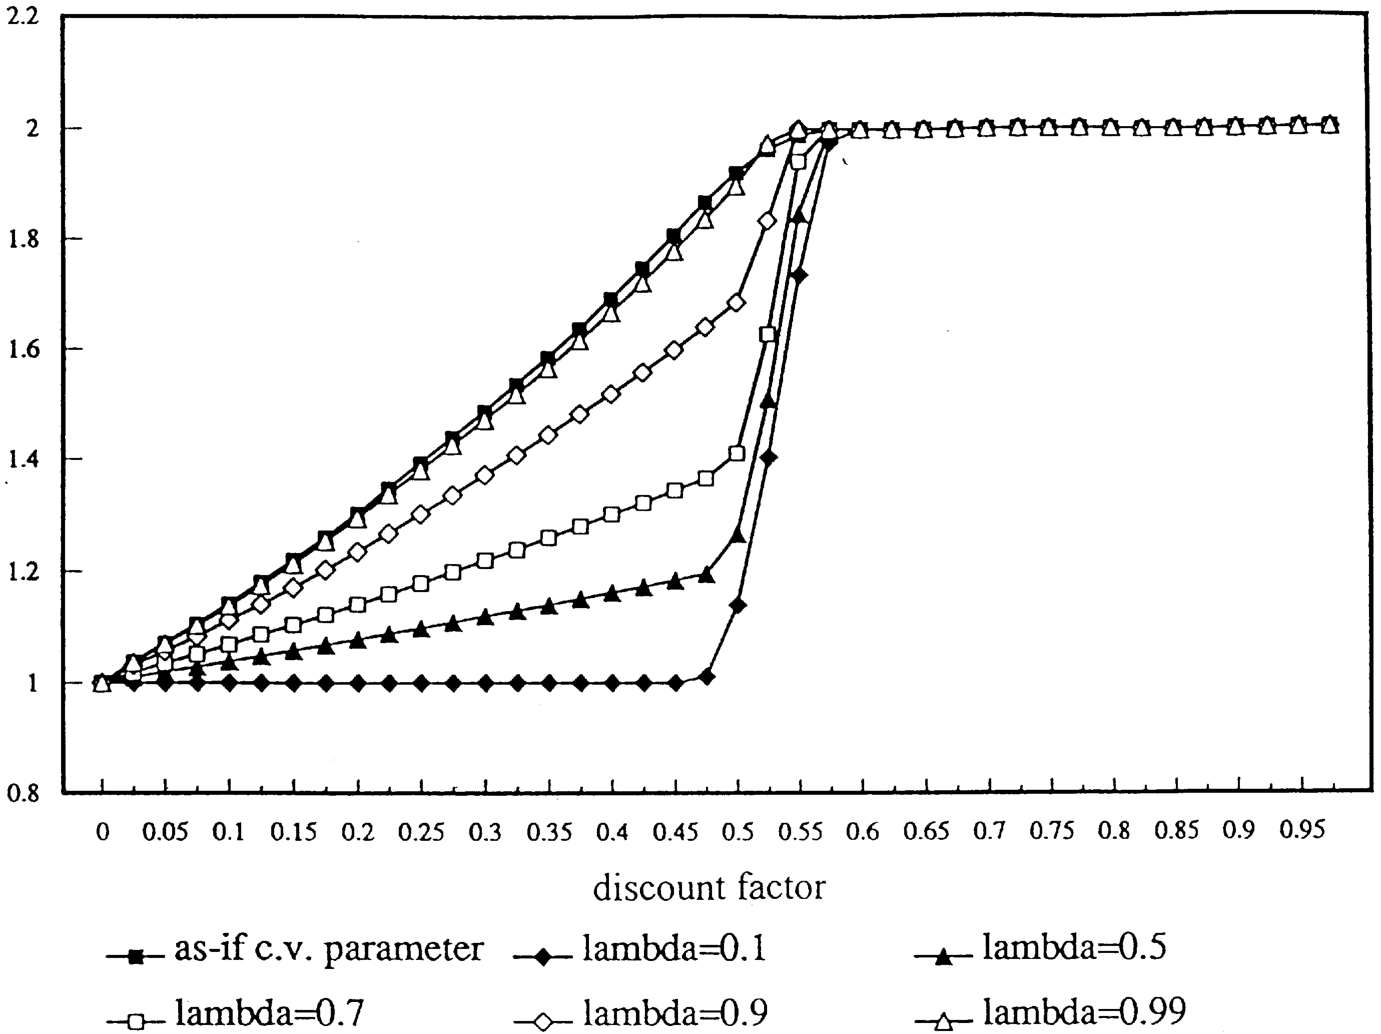
\includegraphics[width=0.85\textwidth]{figures/ch03/corts1999_fig2.png}
\caption[Conduct estimates in Corts's supergame simulations]{Conduct estimates in Corts's supergame simulations with
positively correlated demand, symmetric duopoly. The vertical axis is firm-level conduct (1 is Cournot, 2 is joint
monopoly). The top curve is the as-if conduct parameter. The other curves are conduct parameter estimates for demand
persistence $\varpi$ (``lambda'' in the original) of 0.1, 0.5, 0.7, 0.9 and 0.99. With ten states, $\varpi = 0.1$ makes
demand independent over time. Source: \citet{Corts1999},
Figure~2.}
\label{fig:03-corts-paper-fig2}
\end{figure}

Corts proves the main patterns \citep[Section~3.2]{Corts1999}. If joint monopoly is sustained in every state, the estimate
equals the as-if parameter (his Proposition~2). The monopoly supply relation is itself a conjectural-variations relation,
so it does not matter how monopoly is sustained. If demand is independent over time and monopoly is sustained in no state,
the estimate equals the Cournot value for every such discount factor (Proposition~3). Prices and profits rise with
$\delta$ over this range, yet the method detects none of the collusion. The proof is the one given above, since
$\frac{\dd\tilde q_t}{\dd x_t}$ equals the Cournot response. If demand is fully persistent, the estimate converges to the as-if
parameter (Proposition~4), because $\tilde q_t$ becomes proportional to the demand margin. If a higher demand state shifts
the distribution of future states to the right, the estimate exceeds the Cournot value whenever monopoly is sustained in no
state (Proposition~5). The method then detects some collusion but understates it. With negatively correlated demand, which
resembles seasonal variation, the estimate can fall below the Cournot value even though prices are above it. Corts warns
that seasonal dummies used as demand shifters may then fail to detect collusion, or produce estimates negatively correlated
with true conduct \citep[p.~240]{Corts1999}.

\subsubsection{A worked example: Bertrand collusion with demand shocks}\label{sec:03-corts-bertrand}

The following model is our own illustration, in the spirit of \citet{RotembergSaloner1986} and of Corts. It replaces
Cournot reversion with Bertrand reversion and delivers closed forms. $N$ symmetric firms sell a homogeneous good at constant
marginal cost $c$ and set prices every period. Demand is $Q_t = A_t - P_t$. The demand state $A_t$ is independent and
identically distributed over time with a continuous distribution on $[\underline A, \bar A]$, $\underline A > c$, and firms
observe it before pricing. Firms collude with grim-trigger strategies. Any deviation is followed by pricing at marginal cost
forever, which yields zero profit. Let $\Pi(p, A) = (p - c)(A - p)$ be industry profit and $\pi^m(A) = \frac{(A - c)^2}{4}$
monopoly profit.

\casehead{The incentive constraint}
Suppose firms charge $p \le p^m(A) = \frac{A + c}{2}$ and share the market equally. A deviator undercuts slightly, takes the
whole market and earns almost $\Pi(p, A)$ today and nothing afterward. Colluding yields $\frac{\Pi(p, A)}{N}$ today plus
$\frac{\delta}{1 - \delta}\frac{V}{N}$, where $V = \E[\Pi(p(A'), A')]$ is expected industry profit per period on the
collusive path. The incentive constraint is
\begin{equation*}
\Pi(p, A) - \frac{\Pi(p, A)}{N} \le \frac{\delta}{1 - \delta}\frac{V}{N}
\quad\Longleftrightarrow\quad
\Pi(p, A) \le K \equiv \frac{\delta V}{(1 - \delta)(N - 1)} .
\end{equation*}
Collusion thus caps industry profit at $K$ in every state. A price above $p^m(A)$ is never better. A deviator could then
undercut to $p^m(A)$ and earn $\pi^m(A)$, so the constraint would require $\pi^m(A) \le \frac{\Pi(p, A) + (N - 1)K}{N}$,
which fails whenever $\pi^m(A) > K$. The most profitable sustainable price is therefore
\begin{equation}\label{eq:03-bertrand-price}
p(A) =
\begin{cases}
\frac{A + c}{2} & \text{if } \pi^m(A) \le K ,\\[3pt]
\frac{A + c}{2} - \sqrt{\pi^m(A) - K} & \text{if } \pi^m(A) > K ,
\end{cases}
\end{equation}
where the second line is the lower root of $(p - c)(A - p) = K$. The cap binds in high-demand states, $A > A^* \equiv c +
2\sqrt K$. There the price falls as demand rises. Differentiating the second line,
$\frac{\dd p}{\dd A} = \frac{1}{2} - \frac{A - c}{4\sqrt{\pi^m(A) - K}} < 0$, because $\sqrt{\pi^m(A) - K} < \frac{A - c}{2}$.
These are the price wars during booms of \citet{RotembergSaloner1986}.

\casehead{The equilibrium cap}
Expected industry profit is $V = \E[\min\{\pi^m(A), K\}]$, so the cap solves the fixed-point equation
\begin{equation}\label{eq:03-bertrand-fixed}
K = \nu\, \E\left[\min\{\pi^m(A), K\}\right] \equiv T(K), \qquad \nu \equiv \frac{\delta}{(1 - \delta)(N - 1)} .
\end{equation}

\begin{lemma}[The most collusive equilibrium]\label{lem:03-fixed-point}
(i) If $\delta < 1 - \frac{1}{N}$, the only solution of \eqref{eq:03-bertrand-fixed} is $K = 0$, and firms price at cost.
(ii) If $\delta > 1 - \frac{1}{N}$, there is exactly one positive solution $K^*$. It is the largest fixed point, and the
iteration $K_{n+1} = T(K_n)$ started at any $K_0 \ge \nu\E[\pi^m(A)]$ decreases to $K^*$. (iii) Monopoly pricing in every
state is sustainable if and only if $\nu\,\E[\pi^m(A)] \ge \pi^m(\bar A)$.
\end{lemma}

\begin{proof}
The map $T$ is increasing and concave, because $\min\{\pi^m(A), K\}$ is increasing and concave in $K$ for every $A$. It
satisfies $T(0) = 0$, its right derivative at zero is $\nu$ (since $\pi^m(A) > 0$), and it is bounded by
$\nu\E[\pi^m(A)]$. The condition $\nu < 1$ is equivalent to $\delta < (1 - \delta)(N - 1)$, that is, to $\delta < 1 -
\frac{1}{N}$. (i) If $\nu < 1$, then $T(K) \le \nu K < K$ for every $K > 0$. (ii) If $\nu > 1$, the function
$T(K) - K$ is positive for small $K > 0$ and negative for large $K$, so it has a positive root. It is concave and equals
zero at $K = 0$ with positive slope there. A second positive root would force a concave function to be zero at two points
while positive between zero and the first, which is impossible. Starting at $K_0 \ge \nu\E[\pi^m(A)] \ge K^*$, the
sequence satisfies $K^* = T(K^*) \le T(K_n) \le K_n$, so it decreases and converges to a fixed point no smaller than
$K^*$, which must be $K^*$. (iii) If $K \ge \pi^m(\bar A)$, then $T(K) = \nu\E[\pi^m(A)]$, and the fixed point satisfies
$K \ge \pi^m(\bar A)$ exactly when $\nu\E[\pi^m(A)] \ge \pi^m(\bar A)$.
\end{proof}

Collusion above cost requires $\delta > 1 - \frac{1}{N}$, the familiar condition for Bertrand collusion with constant
demand. It plays the role of condition (i) in \citet{RotembergSaloner1986}, which requires that the number of firms not be
too large relative to the discount factor. They also select the greatest fixed point.
For any $\delta$ above it, the cap exceeds $\pi^m(\underline A)$. If $K \le \pi^m(\underline A)$, then $T(K) = \nu K >
K$, so no fixed point lies there. The lowest demand states are therefore always priced at the monopoly level.

\casehead{Conduct and the conduct parameter estimate}
The markup term is $m_t = Q_t$, because $\lvert\frac{\partial Q}{\partial P}\rvert = 1$. Conduct in state $A$ is
$\theta(A) = \frac{p(A) - c}{Q}$. In unconstrained states $p - c = Q = \frac{A - c}{2}$, so $\theta = 1$. In constrained
states $(p - c)Q = K$, so
\begin{equation*}
\theta(A) = \frac{K}{Q^2}, \qquad P - c = \frac{K}{Q} .
\end{equation*}
Conduct falls as demand rises, and the supply relation in the constrained region is a rectangular hyperbola. Its local
slope is $-\frac{K}{Q^2} = -\theta(A)$. Part (ii) of \cref{prop:03-corts} applies with $Z_t = A_t$, since $m_t = A_t - p(A_t)$
is increasing in $A_t$. The estimate is a weighted average of the local slope $+1$ in unconstrained states and $-\theta(A)$
in constrained states, so it can be negative while every $\theta(A)$ lies in $(0, 1]$.

\Cref{tab:03-corts-sim} and \cref{fig:03-corts-sim} report the numbers for $N = 2$, $c = 0$ and $A_t$ uniform on $[6, 10]$.
Population moments are computed by quadrature, and a regression on 200,000 simulated periods reproduces them to within
$0.002$. Collusion requires $\delta > 0.5$. Monopoly in every state requires $\nu\E[\pi^m(A)] \ge \pi^m(10)$, that is,
$\nu \ge \frac{25}{16.33}$, which holds for $\delta \ge 0.6048$. In between, the cap binds in the high-demand states. At
$\delta = 0.51$, conduct ranges from $0.17$ in the highest state to $1$ in the lowest, and its mean is $0.51$. The
$m$-weighted average conduct is $\frac{\E[P_t - c]}{\E[Q_t]} = \frac{2.34}{5.66} = 0.41$. The instrumental-variables
estimate is $-0.36$. A researcher would conclude that prices lie below the competitive level in an industry whose average
elasticity-adjusted Lerner index is about one half. The estimate turns positive only near $\delta = 0.56$ and catches up with
average conduct when monopoly is sustained everywhere. With $N = 3$ the pattern is the same: at $\delta = 0.677$ mean
conduct is $0.53$ and the estimate is $-0.36$.

\begin{table}[htbp]
\centering
\caption{Mean conduct and the conduct parameter estimate in the Bertrand supergame}
\label{tab:03-corts-sim}
\begin{threeparttable}
\begin{tabular}{@{}cccccc@{}}
\toprule
Discount factor & Profit cap & Cutoff state & Share of states & Mean conduct & IV estimate \\
$\delta$ & $K$ & $A^*$ & constrained & $\E[\theta_t]$ & $\hat\theta$ \\
\midrule
0.5001 & 9.30 & 6.10 & 0.98 & 0.28 & $-0.27$ \\
0.505 & 11.37 & 6.74 & 0.81 & 0.44 & $-0.35$ \\
0.51 & 12.54 & 7.08 & 0.73 & 0.51 & $-0.36$ \\
0.52 & 14.38 & 7.58 & 0.61 & 0.62 & $-0.33$ \\
0.53 & 15.94 & 7.99 & 0.50 & 0.71 & $-0.28$ \\
0.55 & 18.69 & 8.65 & 0.34 & 0.83 & $-0.10$ \\
0.57 & 21.15 & 9.20 & 0.20 & 0.92 & $0.21$ \\
0.6048 & 25.00 & 10.00 & 0.00 & 1.00 & $1.00$ \\
\bottomrule
\end{tabular}
\begin{tablenotes}[flushleft]\footnotesize
\item Notes: $N = 2$ Bertrand firms, marginal cost $c = 0$, demand $Q_t = A_t - P_t$ with $A_t$ independent and uniform on
$[6, 10]$, grim-trigger punishment at marginal cost. $K$ is the largest solution of \eqref{eq:03-bertrand-fixed}, and the
cap binds for $A_t > A^* = 2\sqrt K$. Conduct is $\theta_t = \frac{P_t - c}{Q_t}$, the elasticity-adjusted Lerner index.
The estimate is $\frac{\Cov(A_t, P_t - c)}{\Cov(A_t, Q_t)}$, the limit of the instrumental-variables estimator with a
constant and the demand state as instrument. For $\delta < 0.5$ prices equal cost and both measures are zero. Population
moments computed by quadrature.
\end{tablenotes}
\end{threeparttable}
\end{table}

\begin{figure}[htbp]
\centering
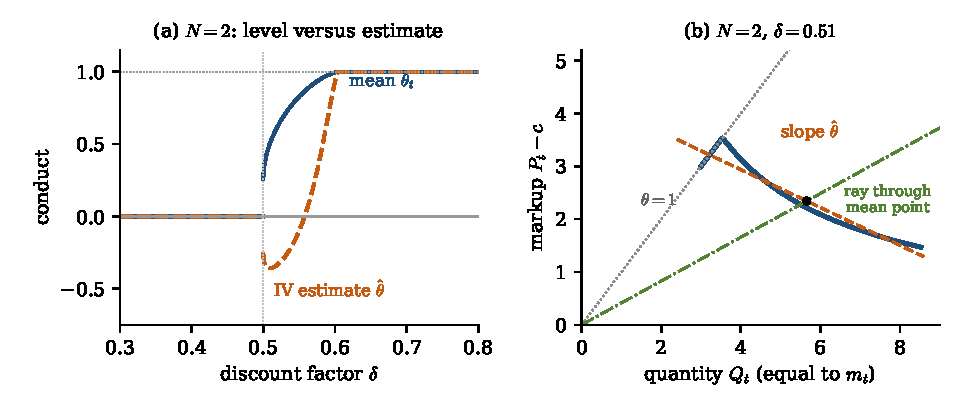
\includegraphics[width=\textwidth]{figures/ch03/corts_sim.pdf}
\caption[Level of conduct versus its estimate in a Bertrand supergame]{Level of conduct versus its estimate in a Bertrand
supergame with independent demand shocks ($N = 2$, $c = 0$, $A_t$ uniform on $[6, 10]$). Panel (a): mean conduct
$\E[\theta_t]$ and the instrumental-variables estimate $\hat\theta$ against the discount factor. Panel (b): the locus of
equilibrium markups and quantities at $\delta = 0.51$. It follows the monopoly ray $\theta = 1$ in low-demand states and the
hyperbola $P - c = \frac{K}{Q}$ in high-demand states. The dashed line through the mean point has slope $\hat\theta = -0.36$,
and the dash-dotted ray through the mean point has slope $0.41$, the $m$-weighted average conduct.}
\label{fig:03-corts-sim}
\end{figure}

The example and Corts's model reach the same conclusion by different routes. With Cournot reversion and independent
shocks, the estimate sticks at the Cournot value. With Bertrand reversion the static benchmark is price taking, and the
constant profit cap makes the constrained supply relation slope downward, so the estimate falls below zero. In both cases
the estimate reflects how the incentive constraint varies with demand, and it carries no direct information on the level
of conduct.

\subsubsection{Assessment}\label{sec:03-corts-assessment}

The critique changes how we read a conduct estimate. A constant-$\theta$ estimate measures the slope of the supply relation,
a weighted average of marginal responses of the markup to demand. Reading it as the level of conduct requires the marginal
and average relations to coincide. This holds in conjectural-variations models, under monopoly in every state, and in the
limit of fully persistent demand. Corts concludes that, when behavior results from efficient supergame collusion, the method
understates market power if demand shocks are not fully permanent. It may detect no market power at all when shocks are
transitory, even with average margins near the monopoly level \citep[pp.~244--245]{Corts1999}.

Three further points follow. First, the specification-test reading does not escape the critique. The estimate can equal
the Cournot value over a wide range of collusive equilibria. A failure to reject Cournot then carries little information,
and tests of the nested static models may lack power. Second, Corts argues that ``not even the positive correlation'' of
the estimate with the as-if parameter can be maintained across models \citep[p.~245]{Corts1999}. Comparisons of conduct
across industries or over time are therefore suspect. Third, the evidence available to Corts points the same way. In the
electricity study of \citet{Wolfram1999} and the sugar study of \citet{GenesoveMullin1998}, the estimates obtained without
cost data fall below the direct measures. Both studies were available to Corts as working papers. Corts notes that equality of the
two can be rejected in both cases \citep[p.~245]{Corts1999}. \Cref{sec:03-sugar,sec:03-electricity} examine both studies.

Genesove and Mullin frame the point in the same terms. The conduct parameter ``measures the marginal response of price, and
hence the markup, to changes in exogenous variables'' \citep[p.~2]{GenesoveMullin1995}. It therefore ``infers market power
from the marginal behavior of the markup, not from the level of the markup.'' They add an example
\citep[p.~3]{GenesoveMullin1995}. Supergame models such as \citet{RotembergSaloner1986} may make the marginal response of
price to demand shifters independent of the discount rate. It is then also independent of the price level at a baseline
state of demand.

The critique has limits. Corts's models are stylized, with linear demand, constant cost, perfect monitoring and an efficient
equilibrium, and the simulations are not calibrated to any industry. They show that the mismeasurement can be severe, and
they leave its size in a given application open. The direction of the bias depends on the persistence of demand, which the
researcher can sometimes measure.

The contribution is lasting. \citet[fn.~7]{BerryHaile2014} cite \citet{Corts1999} and \citet{ReissWolak2007} for the
fundamental problems of the conduct parameter approach. Corts calls for explicit structural models of conduct. The field
responded in three ways. It estimates dynamic models of collusion directly, as in the work on the railroad cartel of
\citet{Porter1983} and \citet{Ellison1994} (\cref{ch:collusion-evidence}). It tests a finite menu of conduct models within
richer demand systems (\cref{sec:03-other-routes}). And it validates the method where marginal cost is observed
(\cref{sec:03-sugar,sec:03-electricity}).

\subsection{Bounds instead of point estimates}\label{sec:03-bounds}

If conduct varies and a constant $\theta$ misleads, we can give up point identification. \citet[Section~2.2]{Rosen2007}
replaces the equilibrium assumption with known bounds on each firm's conduct in each period. The widest bounds are price
taking and monopoly. Conduct may vary freely within them, so the parameters of marginal cost are in general only set identified.
We present the idea in the homogeneous-good setting of this chapter.

Suppose only that industry conduct lies between price taking and joint monopoly, $\theta_t \in [0, 1]$, with no restriction
on how it varies across observations. The supply relation gives $P_t - mc_t = -\theta_t Q_t P'(Q_t)$. Since $-Q_tP'(Q_t)
\ge 0$, the bounds on $\theta_t$ imply $0 \le P_t - mc_t \le -Q_t P'(Q_t)$, that is,
\begin{equation}\label{eq:03-rosen-ineq}
P_t + Q_t P'(Q_t) \;\le\; mc_t \;\le\; P_t .
\end{equation}
Marginal cost lies between monopoly marginal revenue and price, observation by observation. With a parametric marginal
cost $mc_t = c(Q_t, W_t; \beta) + u^s_t$ and $\E[u^s_t \mid X_t] = 0$ for instruments $X_t$, the inequalities become
conditional moment inequalities:
\begin{equation*}
\E\left[P_t - c(Q_t, W_t; \beta) \mid X_t\right] \ge 0, \qquad
\E\left[c(Q_t, W_t; \beta) - P_t - Q_t P'(Q_t) \mid X_t\right] \ge 0 .
\end{equation*}
The \emph{identified set} is the set of $\beta$ that satisfy both for almost every $X_t$. Since $P'(Q_t)$ comes from an
estimated demand curve, estimation has two steps. Bounds on $\beta$ imply bounds on marginal cost, on markups and on each
$\theta_t$, without assuming that conduct is constant.

A deterministic example shows the geometry. Let $mc = b_0 + b_1 Q$ with true values $(b_0, b_1) = (2, 0.5)$, and let
inverse demand in market $t$ be $P = A_t - Q$. Four markets have $A_t = 8, 10, 12, 14$ and conduct $\theta_t = 0.2, 0.9,
0.5, 0.1$. The equilibrium solves $A_t - Q - (2 + 0.5Q) = \theta_t Q$, so $Q_t = \frac{A_t - 2}{1.5 + \theta_t}$. Each
market contributes the two half-planes $P_t - Q_t \le b_0 + b_1 Q_t \le P_t$ in the $(b_1, b_0)$ plane, and we add the
restrictions $b_0 \ge 0$ and $b_1 \ge 0$. \Cref{fig:03-rosen-bounds} shows the intersection. It is a quadrilateral with
$b_1 \in [0, 0.76]$ and $b_0 \in [0.80, 4.47]$. Without the sign restrictions the slope could range from $-1.38$ to $0.76$.
The implied bounds on conduct are informative in some markets. Conduct lies in $[0.66, 1]$ in the second market (true value
$0.9$) and in $[0.36, 0.73]$ in the third (true value $0.5$). In the first and fourth markets only the upper bound moves,
to $0.32$ and $0.42$ (true values $0.2$ and $0.1$).

\begin{figure}[htbp]
\centering
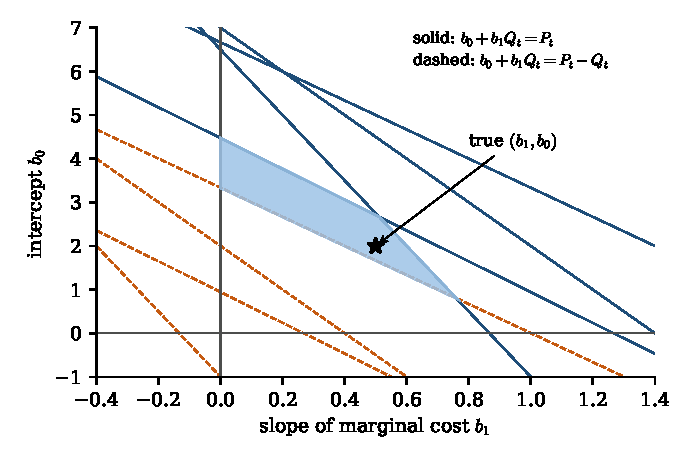
\includegraphics[width=0.60\textwidth]{figures/ch03/rosen_bounds.pdf}
\caption[Identified set for marginal cost when conduct varies freely]{Identified set for a linear marginal cost
$mc = b_0 + b_1 Q$ when conduct varies freely in $[0, 1]$. Each of four markets with inverse demand $P = A_t - Q$ restricts
$(b_1, b_0)$ to the band between a solid line (marginal cost equals price) and a dashed line (marginal cost equals monopoly
marginal revenue). The shaded region is the intersection with $b_0, b_1 \ge 0$. The star marks the true values $(0.5, 2)$.}
\label{fig:03-rosen-bounds}
\end{figure}

The set shrinks quickly when some markets sit near the extremes of conduct. Consider six markets with $A_t = 6, 8, \dots,
16$ and $\theta_t = 0.1, 0.8, 0.3, 1, 0, 0.6$, one of them competitive and one fully collusive. The identified set is then
a small triangle with $b_1 \in [0.33, 0.50]$ and $b_0 \in [2.00, 2.67]$. Every market's conduct is bounded within an
interval of width at most $0.1$. The approach trades precision for robustness. It needs no assumption on how conduct varies,
and it states plainly what the data cannot reveal. Its bounds can be wide, and inference requires methods for moment
inequalities. The Lerner bound \eqref{eq:03-lerner-bound} and Sullivan's bound in \cref{sec:03-sullivan} use the same
logic in reverse. A lower bound on marginal cost, the tax, bounds conduct from above.

\subsection{The record of conduct estimates}\label{sec:03-record}

Almost all estimates of conduct fall strictly between zero and one. The finding is unsurprising, yet it is useful against
extreme claims that an industry is perfectly competitive or fully cartelized. \Cref{tab:01-bresnahan-table} reproduces the
estimated Lerner indices that \citet[Table~17.1]{Bresnahan1989} collected from early studies. \Cref{sec:01-neio-lessons}
discusses the three conclusions he draws from them \citep[pp.~1052--1053]{Bresnahan1989}. He concludes that some
concentrated industries have high margins and that anticompetitive conduct is one cause. He also finds that the studies
reveal little about how market power relates to industry structure.

The entries of that table are margins, and they differ from conduct parameters by the factor $\varepsilon$. Bresnahan left
out studies whose estimates could not be converted into a Lerner index. These include the Panzar-Rosse and Sullivan
methods, which yield tests or bounds, and the residual demand method, whose elasticities equal the Lerner index only in
special cases \citep[fn.~47]{Bresnahan1989}. Two lessons of this section qualify the record further. A conduct estimate is
a slope, so estimates in $(0, 1)$ are compatible with conduct that swings between collusion and price wars
(\cref{sec:03-corts}). The most direct test of the methods compares them with observed costs, which is the task of
\cref{sec:03-sugar,sec:03-electricity}.

\section{Sugar refining, 1890--1914: Genesove and Mullin (1998)}\label{sec:03-sugar}

The methods of \cref{sec:03-sumner,sec:03-identification} infer market power without observing marginal
cost. Their answers are only as good as the maintained assumptions on demand, cost and conduct. Whether
those assumptions deliver the right answer in a real industry is an empirical question.
\citet{GenesoveMullin1998} answer it for American cane sugar refining between 1890 and 1914, an industry in
which marginal cost can be measured almost directly. They compute conduct twice. The first computation uses
the cost information and serves as a benchmark. The second treats cost as unknown and applies the standard
estimator of the New Empirical Industrial Organization (NEIO). Together with the electricity study of
\cref{sec:03-electricity}, this comparison is the closest the literature comes to a controlled test of the
conduct-parameter method.\footnote{We work from two versions. The article \citep{GenesoveMullin1998} is
cited by its table numbers (``Table 2'') and its published page numbers. The working paper \citep{GenesoveMullin1995} contains a longer
history, the cost evidence and several tables that the article omits. We cite those as ``WP Table 9'' and
give its printed page numbers. Published Tables 2, 3 and 4 correspond to WP Tables 4, 6, and 7 and 8.
Published Table 10 reproduces two columns of WP Table 14 with a different direct measure. Published Table 9
has no counterpart in the working paper.}

\subsection{The question and why sugar}\label{sec:03-sugar-question}

Genesove and Mullin start from the supply relation \eqref{eq:03-supply-relation} with a constant marginal
cost $c$,
\begin{equation}\label{eq:03-gm-supply}
P + \theta\, Q\, P'(Q) = c ,
\end{equation}
and from its Lerner form \eqref{eq:03-lerner-theta}, $\theta = \varepsilon(P)\frac{P - c}{P} \equiv
L_\varepsilon$. With complete cost information and an estimated demand elasticity, the elasticity-adjusted
Lerner index delivers $\theta$ period by period. Without cost information, $\theta$ must be restricted,
because an unrestricted $\theta_t$ fits any data (\cref{prop:03-exact-fit}). The usual restriction is that
$\theta$ is constant, or at least uncorrelated with the instruments (WP p.~4).

Three features make sugar refining the right place for a test (WP pp.~3--4). First, the technology is
simple. Raw sugar is turned into refined sugar at a fixed and known coefficient, both prices are observed,
and the remaining costs are documented. A true price-cost margin can therefore be computed. Second, the
harvest cycle of raw sugar and year-to-year weather generate supply variation that is plausibly exogenous to
American demand. This variation helps identify demand and, through it, conduct. Third, the industry went
through dramatic structural changes: the formation of a trust, repeated entry with price wars, renewed
consolidation, and an antitrust prosecution. These episodes let us ask whether estimated conduct moves with
structure, and whether the method can tell a change in conduct from a change in cost.

The test answers two standing objections to the NEIO (WP pp.~2--3). The first is that functional forms for
demand impose strong restrictions on the relation between price and marginal cost. The second is the point
of \citet{Corts1999} developed in \cref{sec:03-corts}. The estimated conduct parameter measures the marginal
response of the markup to the identifying shocks, and so may misstate its level. Genesove and Mullin note
that no NEIO estimate had ever been checked against an independent measure of conduct. Their design makes
three comparisons. The NEIO estimate $\hat\theta$ is compared with the direct measure $L_\varepsilon$. The
NEIO estimates of the cost parameters are compared with their documented values. Finally, the estimates for
different structural regimes are compared with the direct measures for the same regimes. Throughout, the
maintained hypothesis is that $L_\varepsilon$ measures conduct without error (WP p.~5).

\subsection{The industry, 1887--1914}\label{sec:03-sugar-history}

The American cane sugar refining industry of this period combined high concentration with repeated entry.
\Cref{tab:03-gm-chronology} lists the main events (WP Tables 1 and 13). The account below follows WP
pp.~6--8 and 13--15. These pages rely on \citet{Eichner1969}, \citet{Zerbe1969} and Willett and Gray's
\emph{Weekly Statistical Sugar Trade Journal}, the source of most of the data.

\begin{table}[htbp]
\centering
\caption{Chronology and structural regimes of the U.S. sugar refining industry}\label{tab:03-gm-chronology}
\small
\begin{tabular}{@{}ll@{}}
\toprule
\multicolumn{2}{@{}l}{\textit{Panel A. Events (WP Table 1 and text)}}\\
\midrule
1887 (Dec.) & Sugar Trust formed: 18 firms with 80 percent of capacity\\
1889--1890 & Entry by Spreckels (Philadelphia plant completed in Dec. 1889), price war\\
1891 & Trust reorganized as the American Sugar Refining Company (ASRC)\\
1891--1892 & Acquisition of Spreckels and others, ASRC reaches 95 percent of capacity\\
1892--1896 & Small-scale entry by five single-plant firms, cartel operation\\
1898 & Entry by Arbuckle Brothers (August) and Doscher (November)\\
1900 (May) & End of the Arbuckle war\\
1903 & Cuban Reciprocity Treaty: Cuban raw sugar enters at 80 percent of full duty\\
1910 & Federal antitrust suit (consent decree in 1922)\\
1914 & World War I begins, the sample ends in June 1914\\
\midrule
\multicolumn{2}{@{}l}{\textit{Panel B. Regimes used in the estimation (WP Table 13)}}\\
\midrule
Jan. 1890 to Feb. 1892 & Spreckels entry, price war\\
Mar. 1892 to Sep. 1898 & Acquisition of Spreckels, small-scale entry, cartel operation\\
Sep. 1898 to Apr. 1900 & Entry by Arbuckle Brothers and Doscher, price war\\
May 1900 to 1910 & After the Arbuckle war\\
Nov. 1910 to 1913 & Government antitrust suit\\
\bottomrule
\end{tabular}

\smallskip
\begin{minipage}{0.92\textwidth}\footnotesize
Notes: Compiled from \citet{GenesoveMullin1995}, WP Tables 1 and 13 and pp.~6--8. The two price-war regimes
in Panel B are the ``post-entry price wars'' of \cref{sec:03-sugar-wars}.
\end{minipage}
\end{table}

\casehead{Trust and first entry}
After several failed attempts at collusion, the Sugar Trust was formed in December 1887. It consolidated 18
firms that controlled 80 percent of industry capacity, and it soon reduced their 20 plants to 10. The
average refined price rose about 16 percent, from \$6.013 per hundred pounds in 1887 to \$7.007 in 1888 (WP
p.~6, fn.~2). Entry followed. Claus Spreckels, a West Coast refiner, completed a plant in Philadelphia in
December 1889, in retaliation for the Trust's purchase of a California refinery. A price war ensued. The
Trust, reorganized in 1891 as the American Sugar Refining Company (ASRC), then bought the Spreckels plant
and the remaining outsiders. By April 1892 it held 95 percent of capacity. Genesove and Mullin describe this
episode as the template for the period: high concentration, punctuated by entry, price wars, and then
acquisition of or accommodation with the entrants (WP p.~7).

\casehead{Cartel and second entry}
Between 1892 and 1896 five firms entered, each with a single plant of about 1,340 barrels of refined sugar
per day on average. ASRC and its ``friendly'' companies had 49,500 barrels per day. ASRC acted as cartel
leader, and by 1896 an understanding with the independents had evolved. The next challenge came from the
Arbuckle Brothers, wholesale grocers and the dominant American coffee roasters. Their refinery began limited
production in August 1898, and the Doscher refinery started in November. Each plant had a capacity of 3,000
barrels per day. A severe price war followed, with pricing at or below cost, shutdowns by independent
refiners and partial exit of one entrant. Apart from one respite, the war lasted until May 1900. It ended
when Doscher merged with two major independents in a transaction organized by the president of ASRC (WP
pp.~7--8).

\casehead{Tariffs, antitrust and fringes}
The tariff on refined sugar protected domestic refiners from European competition. From 1903, the Cuban
Reciprocity Treaty admitted Cuban raw sugar at 80 percent of the full duty. In antitrust, the government
challenged ASRC's purchase of several Philadelphia refineries in 1892, and the Supreme Court upheld the
acquisition in 1895 (the \emph{E.\,C.~Knight} case). In 1910 the federal government sued for dissolution.
The case ended in a consent decree only in 1922, but after the government's victories against Standard Oil
and American Tobacco in 1911, ASRC began a partial ``voluntary'' dissolution (WP p.~8). Two competitive
fringes disciplined the cane refiners. Domestic beet sugar supplied less than 1 percent of consumption until
1894, 5 percent by 1901 and 15 percent in 1908--1914. European beet refiners were a threat of imports, and
ASRC's president testified in 1888 and 1894 that ASRC set prices so that no refined sugar would be imported
(WP p.~14). Genesove and Mullin do not model the fringes. Their conduct measures are therefore ``overall''
measures that include the discipline of potential imports and beet sugar (WP p.~15).

\casehead{Product, sunk costs and capacity}
The standard grade of refined sugar, ``standard granulated,'' was a homogeneous product. Refiners shipped it
to grocers in barrels, and grocers repackaged it without identifying the manufacturer, so prices tended to
uniformity (WP pp.~13--14). A refinery of 3,000 barrels per day cost between \$1.5 and \$2.5 million in 1900.
Plant and machinery had little value outside sugar, while the waterfront land had considerable salvage value.
Entry costs were thus largely, but not completely, sunk. Industry output stayed well below capacity
throughout, and ASRC kept excess capacity even in the depths of the Arbuckle war (WP p.~13). ASRC's share
of the market fell from 91 percent in 1892 to 43 percent in 1914 (WP Table 9).

\subsection{Technology and the direct measurement of marginal cost}\label{sec:03-sugar-cost}

Refined sugar was made mostly from cane. Cane was first processed into raw sugar, which could be shipped
and stored. The standard grade, ``96 degree centrifugals,'' was 96 percent sucrose, and its sugar content
was tested with a polariscope, which made the input homogeneous. Most raw sugar came from the tropics,
especially Cuba, with Louisiana the main domestic source. Refiners melted, purified and crystallized it
into refined sugar, which is pure sucrose. Witnesses for both ASRC and an independent testified that all
refiners used a common process (WP p.~9).

\begin{assumption}[Fixed-coefficient technology]\label{ass:03-gm-cost}
The marginal cost of producing one hundred pounds of refined sugar in period $t$ is
\begin{equation}\label{eq:03-gm-cost}
c_t = c_0 + k\,P^{\mathrm{raw}}_t .
\end{equation}
Here $P^{\mathrm{raw}}_t$ is the price of one hundred pounds of raw sugar, and $k$ is the quantity of raw sugar
needed per unit of refined sugar. The term $c_0$ collects all other variable costs (labor, fuel, boneblack,
packages, brokerage, net of the value of byproducts). Both $c_0$ (in constant dollars) and $k$ are constant
over time and do not depend on output.
\end{assumption}

The assumption that marginal cost does not depend on output is natural in an industry that always operated
well below capacity. Genesove and Mullin maintain \eqref{eq:03-gm-cost} throughout, and then measure $k$ and
$c_0$ from engineering and testimonial evidence.

\casehead{The input coefficient}
Raw sugar is 96 percent sucrose, so the physical minimum is $k = \frac{1}{0.96} = 1.042$. The working paper
truncates this value and prints 1.041 (WP p.~10). Some sugar is lost
in refining. A Treasury commission found in 1898 that one hundred pounds of raw sugar yielded 92.5 pounds of
refined sugar. Genesove and Mullin put the yield at 92.5 to 93 pounds (WP p.~10). One pound of refined sugar
therefore requires about $\frac{1}{0.93} = 1.075$ pounds of raw sugar, and Genesove and Mullin set
$k = 1.075$. Audits of refiners' books by the Tariff Commission show that the coefficient did not change
during the sample period or after it.

\casehead{Non-sugar costs}
The trade spoke of ``the margin,'' the difference between the refined and the raw price. Because $k > 1$,
that margin overstates the money left after paying for raw sugar. The relevant quantity is the \emph{proper
margin}
\begin{equation}\label{eq:03-gm-proper-margin}
G_t \equiv P_t - k\,P^{\mathrm{raw}}_t = c_0 + (P_t - c_t),
\end{equation}
the refined price net of raw-sugar cost (WP pp.~10--11). By \eqref{eq:03-gm-cost}, the proper margin equals
non-sugar cost plus the price-cost margin. Five pieces of evidence pin down $c_0$, all expressed in constant
1898 dollars per hundred pounds.
\begin{enumerate}[label=(\roman*)]
\item The earliest evidence is testimony before the Industrial Commission in June 1899 (WP pp.~10--11). Henry
Havemeyer, president of ASRC, said that he had never known a cost of refining below one-half cent a pound. At the
formation of the trust it had been three-quarters of a cent. He agreed that at a margin of 50 cents a hundred pounds
``the refineries are running at a loss'' (WP p.~10, fn.~14). James Jarvie, a partner of Arbuckle Brothers, put the
cost of refining at ``50 to 60 points, or one-half to six-tenths of a cent per pound.'' He added that ``if raw sugar
costs $4\frac{1}{2}$ cents a pound, it will cost over 5 cents up to $5\frac{10}{100}$'' (WP p.~11, fn.~15). The raw price in this statement is hypothetical. Subtracting its raw-sugar cost from the two
totals gives, per hundred pounds,
\begin{equation*}
c_0 = 500 - 1.075 \times 450 = 16.25 \text{ cents},
\qquad
c_0 = 510 - 1.075 \times 450 = 26.25 \text{ cents}.
\end{equation*}
\item Another witness itemized non-sugar costs: 5 cents for brokerage and taxes, 10 cents for packages and
20 cents for wages, fuel, boneblack, repairs and sundries, less 10 cents of byproduct (syrup) revenue. The
total is 25 cents.
\item At the Hardwick Committee hearings of 1911, refiners quoted a refining cost of 60 to 65 cents when raw
sugar sold for \$4.00. A refining cost in this sense is $c - P^{\mathrm{raw}} = c_0 + (k - 1)P^{\mathrm{raw}}$,
so $c_0$ lies between $60 - 0.075 \times 400 = 30$ and $35$ cents in current dollars, or 22 to 26 cents in
1898 dollars.
\item Tariff Commission audits for 1914 give a total refinery cost of \$0.420. Removing \$0.013 of accounting
depreciation and \$0.056 of byproduct receipts leaves \$0.351 in current dollars, or 25 cents in 1898
dollars (WP p.~11, fn.~18).
\item Behavior during the Arbuckle war bounds $c_0$ as well. The independents shut down or ran at
``minimum capacity'' at times. The minimum proper margin above which they always produced was 26 cents, and
except for a couple of weeks they never produced below 9 cents. For example, they shut down when the refined
price was \$4.71 and the raw price \$4.30, a proper margin of $4.71 - 1.075 \times 4.30 = 0.0875$ (WP p.~12,
fn.~22).
\end{enumerate}
Shutdown behavior cannot reveal a single break-even margin (WP p.~12). Prices are observed only on Fridays.
Month-long contracts and the value of a reputation for reliable supply can justify producing at a loss. Costs
of shutting down and restarting open a band of margins in which a firm sometimes produces and sometimes does
not. The band is consistent with the direct estimates, however.

Genesove and Mullin adopt $c_0 = 0.26$, the value supported by the most and best evidence, and use $0.16$ as a
lower bound. The range reflects the researchers' ignorance. Cost differences among firms were small: a commission
merchant for an independent refiner estimated that larger houses might refine 3 to 5 cents more cheaply
(WP pp.~12--13). Non-sugar inputs are small:
4.5 percent of cost at $c_0 = 0.16$ and 7.5 percent at $c_0 = 0.26$ (WP p.~12). The direct measure of
marginal cost is therefore
\begin{equation}\label{eq:03-gm-direct-cost}
c_t = 0.26 + 1.075\,P^{\mathrm{raw}}_t .
\end{equation}
More than nine tenths of marginal cost is an observed input price that fluctuates a great deal. This is
what makes sugar refining so well suited to a validation exercise.

\subsection{Data, instruments and the demand system}\label{sec:03-sugar-demand}

\casehead{Data}
The sample is quarterly, from January 1890 to June 1914 (WP p.~26). Prices come from Willett and Gray's
weekly quotations. Consumption data do not exist, so quantity is measured by \emph{meltings} $M_t$, the
quantity of raw sugar melted by refiners. Meltings track consumption closely because refined sugar
deteriorates in storage and refiners produced to order with about a one-month lag (WP pp.~16--17). Prices are
in dollars per hundred pounds, deflated to constant 1898 dollars with the wholesale price index of
\citet{Hanes1993}. Meltings and Cuban imports are in hundreds of thousands of long tons per quarter. Cuban
imports were zero in the third quarter of 1897, during the Cuban war of independence, and that quarter is
dropped \citep[pp.~365, 373]{GenesoveMullin1998}. This leaves 97 quarters: 73 in the low season and 24 in
the high season defined below. \Cref{tab:03-gm-stats} reports the sample statistics.

\begin{table}[htbp]
\centering
\caption{Sample statistics, quarterly, 1890--1914}\label{tab:03-gm-stats}
\small
\begin{tabular}{@{}lcccccc@{}}
\toprule
 & \multicolumn{2}{c}{Full sample} & \multicolumn{2}{c}{Low season} & \multicolumn{2}{c}{High season}\\
\cmidrule(lr){2-3}\cmidrule(lr){4-5}\cmidrule(l){6-7}
 & Mean & S.D. & Mean & S.D. & Mean & S.D.\\
\midrule
Refined price $P$ & 4.03 & 0.62 & 3.99 & 0.63 & 4.14 & 0.58\\
Raw price $P^{\mathrm{raw}}$ & 3.30 & 0.59 & 3.28 & 0.61 & 3.36 & 0.53\\
Proper margin $P - 1.075\,P^{\mathrm{raw}}$ & 0.48 & 0.19 & 0.46 & 0.18 & 0.53 & 0.21\\
Meltings $M$ & 4.43 & 1.11 & 4.20 & 1.04 & 5.11 & 1.07\\
Cuban imports & 2.18 & 1.73 & 2.28 & 1.88 & 1.87 & 1.13\\
Observations & \multicolumn{2}{c}{97} & \multicolumn{2}{c}{73} & \multicolumn{2}{c}{24}\\
\bottomrule
\end{tabular}

\smallskip
\begin{minipage}{0.92\textwidth}\footnotesize
Notes: Reproduced from \citet{GenesoveMullin1998}, Table 2 (identical to WP Table 4). Prices in constant
1898 dollars per hundred pounds. Quantities in hundreds of thousands of long tons. The high season is the
third quarter.
\end{minipage}
\end{table}

Three facts stand out. Meltings are 22 percent higher in the high season ($\frac{5.11}{4.20} = 1.22$), while
the refined price is only 15 cents higher and the raw price 8 cents higher. The proper margin rises by about
7 cents between the seasons. Finally, the mean proper margin less $c_0 = 0.26$ is $0.48 - 0.26 = 0.22$,
which is $\frac{0.22}{4.03} = 0.055$ of the mean price. Price exceeded marginal cost by only about 5
percent.

\casehead{Frequency}
Weekly data were available, but Genesove and Mullin use quarterly data on purpose (WP p.~16). With switching
costs for grocers or consumers, short-run demand is less elastic than long-run demand. A high-frequency
elasticity would imply a monopoly price far above what a forward-looking monopolist would charge. Observed
prices would then look very competitive, and market power would be understated. Quarterly data are a
compromise. Monthly data give qualitatively similar estimates.

\casehead{The supply instrument}
Demand estimation needs a variable that shifts supply but not demand. The raw sugar price is the obvious
cost shifter, but the United States consumed about 25 percent of the world's sugar. A shock to American
demand therefore moved the world raw price, which makes the raw price an invalid instrument (WP p.~17).
Genesove and Mullin instrument instead with \emph{Cuban imports} of raw sugar. Cuba was the closest and,
after 1903, the tariff-preferred source of raw sugar for the East Coast refiners. Four arguments support
exogeneity (WP pp.~17--23).
\begin{enumerate}[label=(\alph*)]
\item Cuban exports went almost entirely to the United States. The share never fell below 85 percent and
exceeded 98 percent in every year from 1900 to 1909 (WP Table 2). Cuban imports were inframarginal for the
American market. The next destination, London, involved much higher shipping costs and the switching costs
of an industry organized around New York.
\item The sources of variation in Cuban supply were the seasonal harvest cycle, yearly weather, the war of
independence of 1895--1898 with the Spanish-American War, and a secular increase in cane planting. The first
three are exogenous to American demand. Cuban production fell from 1,004,264 tons in 1895 to 225,221 in 1896
and 212,051 in 1897 (WP Table 2). Much of the secular expansion responded to the 1903 treaty, a time trend
in demand absorbs the rest, and cane yields harvests for five years with little tending.
\item A negative American demand shock could induce Cuban suppliers to hold sugar back for a later quarter.
This was impractical. Raw sugar was not warehoused in Cuba because the hot climate caused deterioration,
and speculative storage took place in New York, which leaves imports unaffected. Delaying the harvest lost
sucrose and risked the onset of the rainy season, which made the roads impassable.
\item Quarterly aggregation further weakens any incentive to shift imports between periods.
\end{enumerate}

\casehead{A flexible family of demand curves}
Genesove and Mullin specify industry demand as
\begin{equation}\label{eq:03-gm-demand}
Q(P) = \beta\,(\alpha - P)^{\gamma} .
\end{equation}
In this section only, $\alpha$, $\beta$ and $\gamma$ denote these demand parameters, to match the paper. They
are unrelated to the price coefficient and taste parameters of the discrete-choice chapters. The parameter
$\beta > 0$ scales the market, $\gamma$ indexes convexity, and for $\gamma > 0$ the parameter $\alpha$ is the
choke price. The next lemma collects the properties we use.

\begin{lemma}[Properties of the demand family]\label{lem:03-gm-demand}
For \eqref{eq:03-gm-demand} with $\gamma > 0$ and $P < \alpha$, or with $\alpha = 0$ and $\gamma < 0$, in which case
we read the family as $Q = \beta P^{\gamma}$, the following hold.
\begin{enumerate}[label=(\roman*)]
\item The price elasticity is $\varepsilon(P) = \frac{\gamma P}{\alpha - P}$, and the markup term is
$m(P) \equiv \frac{Q(P)}{\lvert Q'(P)\rvert} = \frac{\alpha - P}{\gamma}$.
\item The family contains the quadratic ($\gamma = 2$), the linear ($\gamma = 1$) and the log-linear or
constant-elasticity form ($\alpha = 0$, $\gamma < 0$, with $\varepsilon = -\gamma$). As $\alpha, \gamma \to
\infty$ with $\frac{\gamma}{\alpha} = \lambda$ fixed (a local symbol, unrelated to the composite slope of
\cref{sec:03-identification}), demand converges to the exponential form
$Q \propto e^{-\lambda P}$, with $\varepsilon = \lambda P$ and $m = \frac{1}{\lambda}$.
\item The curvature of inverse demand, $\chi \equiv -\frac{Q P''(Q)}{P'(Q)}$, equals $1 - \frac{1}{\gamma}$.
\end{enumerate}
\end{lemma}

\begin{proof}
(i) Differentiate \eqref{eq:03-gm-demand}: $Q'(P) = -\gamma\beta(\alpha - P)^{\gamma - 1}$. Then
\begin{equation*}
\varepsilon(P) = -\frac{Q'(P)\,P}{Q(P)} = \frac{\gamma\beta(\alpha - P)^{\gamma - 1} P}{\beta(\alpha - P)^{\gamma}}
= \frac{\gamma P}{\alpha - P},
\qquad
\frac{Q(P)}{\lvert Q'(P)\rvert} = \frac{\beta(\alpha - P)^{\gamma}}{\gamma\beta(\alpha - P)^{\gamma - 1}}
= \frac{\alpha - P}{\gamma}.
\end{equation*}
In the case $\alpha = 0$, $\gamma < 0$, demand is $Q = \beta P^{\gamma}$, so $Q' = \gamma\beta P^{\gamma - 1}$,
$\varepsilon = -\gamma$ and $\frac{Q}{\lvert Q'\rvert} = -\frac{P}{\gamma}$, which equals $\frac{\alpha - P}{\gamma}$ at
$\alpha = 0$.
(ii) The first three cases are immediate. For the limit, write $\gamma = \lambda\alpha$ and
\begin{equation*}
(\alpha - P)^{\gamma} = \alpha^{\gamma}\left(1 - \frac{P}{\alpha}\right)^{\lambda\alpha}
\;\longrightarrow\; \alpha^{\gamma}\, e^{-\lambda P}
\qquad (\alpha \to \infty),
\end{equation*}
using $\left(1 - \frac{x}{n}\right)^{n} \to e^{-x}$. The factor $\alpha^{\gamma}$ is absorbed into the
scale. The elasticity and markup term follow from (i):
$\frac{\gamma P}{\alpha - P} = \frac{\lambda P}{1 - \frac{P}{\alpha}} \to \lambda P$ and
$\frac{\alpha - P}{\gamma} = \frac{1}{\lambda} - \frac{P}{\gamma} \to \frac{1}{\lambda}$.
(iii) Inverse demand is $P(Q) = \alpha - \left(\frac{Q}{\beta}\right)^{\frac{1}{\gamma}}$. Hence
\begin{equation*}
P'(Q) = -\frac{1}{\gamma}\,\beta^{-\frac{1}{\gamma}}\,Q^{\frac{1}{\gamma} - 1},
\qquad
P''(Q) = -\frac{1}{\gamma}\left(\frac{1}{\gamma} - 1\right)\beta^{-\frac{1}{\gamma}}\,Q^{\frac{1}{\gamma} - 2},
\end{equation*}
and $-\frac{QP''(Q)}{P'(Q)} = -\left(\frac{1}{\gamma} - 1\right) = 1 - \frac{1}{\gamma}$. In the case $\alpha = 0$,
$\gamma < 0$, inverse demand is $P(Q) = \left(\frac{Q}{\beta}\right)^{\frac{1}{\gamma}}$. Both derivatives change sign,
and their ratio is unchanged.
\end{proof}

Part (iii) places the family inside the pass-through analysis of \cref{sec:03-passthrough-theory}. Linear
demand has $\chi = 0$, quadratic demand $\chi = \frac{1}{2}$, exponential demand $\chi = 1$ and
constant-elasticity demand $\chi = 1 + \frac{1}{\varepsilon}$. The four forms thus span the curvatures that
\cref{prop:03-passthrough} shows to matter for the link between pass-through and conduct.

\casehead{Seasons as a demand rotator}
Sugar is a complement of fruit in canning. The canning season begins at the end of May with the first New
York strawberries and peaks in September (WP p.~24). Genesove and Mullin define the indicator $H_t = 1$ in
the third quarter and $H_t = 0$ otherwise, and call the third quarter the \emph{high season}. Write
$s(t) \in \{L, H\}$ for the season of quarter $t$. Both the scale $\beta$ and one shape parameter ($\alpha$,
$\gamma$ or $\frac{\gamma}{\alpha}$, depending on the form) may differ by season. The high season can
therefore raise demand proportionally and also change the monopoly price (WP p.~25). A change in $\beta$
alone moves quantity at every price but leaves the markup term $m(P) = \frac{\alpha - P}{\gamma}$ unchanged.
What identifies conduct here is a seasonal change in $m(P)$ at given prices, that is, in the elasticity of
demand at a given price. Because marginal cost is assumed constant in output, such a change is enough, even
when it is a parallel shift of linear demand (\cref{sec:03-other-routes}). In the estimates below, the high
season changes both the level and the slope of demand, so canning demand also rotates it.

\casehead{Estimating equations}
For each season $s$, the four forms give the estimating equations (WP eqs.~6--9)
\begin{align}
\text{Quadratic:}\quad & \ln M_t = b_s + 2\ln(\alpha_s - P_t) + e_t, \label{eq:03-gm-quad}\\
\text{Linear:}\quad & M_t = \beta_s\alpha_s - \beta_s P_t + e_t, \label{eq:03-gm-lin}\\
\text{Log-linear:}\quad & \ln M_t = b_s + \gamma_s \ln P_t + e_t, \label{eq:03-gm-loglin}\\
\text{Exponential:}\quad & \ln M_t = b_s - \lambda_s P_t + e_t. \label{eq:03-gm-exp}
\end{align}
The constant $b_s$ is the logarithm of the season's scale.\footnote{The working paper writes the constant as
$-\ln\beta$. Only the estimated constant matters for what follows.} In the three logarithmic forms the error
$e_t$ is a proportional shift of demand, a shift in $\beta$. By \eqref{eq:03-gm-cost} and the pricing rule
derived below, such a shift does not move the profit-maximizing price at any $\theta$. Demand shocks
therefore do not enter the pricing equation, which justifies treating the two errors as uncorrelated later
on.

The refined price is endogenous in \eqref{eq:03-gm-quad}--\eqref{eq:03-gm-exp}. Within each season the
instruments $z^d_t$ are a constant and the logarithm of Cuban imports, $\ln\mathit{CUBA}_t$
\citep[Table~3, notes]{GenesoveMullin1998}. The moment conditions are $\E[e_t\, z^d_t] = 0$.
Each season's equation has two parameters and two instruments, so the estimator is exactly identified. The quadratic form is nonlinear in $\alpha_s$ and is
estimated by nonlinear instrumental variables \citep{Amemiya1985}. Standard errors are robust to
heteroskedasticity and to serial correlation of up to four lags \citep{NeweyWest1987}. The pooled
specification of WP Table 5 adds a linear time trend in $\ln\beta$ and interacts price with $H_t$. Its trend
coefficients are negative and insignificant, which Genesove and Mullin attribute to the spread of beet sugar
(WP p.~26). The joint tests that both high-season terms are zero give $\chi^2_{(2)}$ statistics of 4.91,
22.73, 23.40 and 20.77 for the four forms (WP Table 5). Dropping the trend allows estimation season by season, which gives \cref{tab:03-gm-demand}. All
later calculations use these by-season estimates.

\begin{table}[htbp]
\centering
\caption{Demand for refined sugar, estimated separately by season}\label{tab:03-gm-demand}
\small
\begin{tabular}{@{}lcccc@{}}
\toprule
 & (1) Quadratic & (2) Linear & (3) Log-linear & (4) Exponential\\
 & $\gamma = 2$ & $\gamma = 1$ & $\alpha = 0$ & $\gamma, \alpha \to \infty$\\
\midrule
\multicolumn{5}{@{}l}{\textit{Low season} ($N = 73$)}\\
Price coefficient & $\alpha_L = 7.72$ & $-\beta_L = -2.30$ & $\gamma_L = -2.03$ & $-\lambda_L = -0.53$\\
 & (0.86) & (0.48) & (0.48) & (0.12)\\
Intercept & $-1.20$ & $\beta_L\alpha_L = 13.37$ & 4.19 & 3.52\\
 & (0.47) & (1.90) & (0.65) & (0.48)\\
\addlinespace
\multicolumn{5}{@{}l}{\textit{High season} ($N = 24$)}\\
Price coefficient & $\alpha_H = 11.88$ & $-\beta_H = -1.36$ & $\gamma_H = -1.10$ & $-\lambda_H = -0.26$\\
 & (2.03) & (0.36) & (0.28) & (0.07)\\
Intercept & $-2.48$ & $\beta_H\alpha_H = 10.74$ & 3.17 & 2.70\\
 & (0.54) & (1.57) & (0.40) & (0.29)\\
\addlinespace
$\chi^2_{(2)}$ test of equality across seasons & 6.90 & 28.18 & 29.17 & 25.96\\
\bottomrule
\end{tabular}

\smallskip
\begin{minipage}{0.92\textwidth}\footnotesize
Notes: Reproduced from \citet{GenesoveMullin1998}, Table 3, which prints each price coefficient next to the
parameter it identifies (the quadratic column reports the choke price $\alpha_s$ itself). Instrument: log of
Cuban imports. Newey-West standard errors (four lags) in parentheses. The $\chi^2_{(2)}$ statistic tests
equality of the price and intercept coefficients across seasons. WP Table 6 is identical except for three
rounding differences: 0.87 for the first standard error, and 4.18 and 3.16 for the log-linear intercepts.
\end{minipage}
\end{table}

\casehead{Reading the demand estimates}
Every form agrees that the high season both shifts demand out and makes it less elastic. The
$\chi^2_{(2)}$ statistics reject equality across seasons at the 5 percent level in the quadratic form
(cutoff 5.99) and at below 1 percent in the other three. In the linear form the two demand curves are
$M = 13.37 - 2.30P$ and $M = 10.74 - 1.36P$. They cross at $P = \frac{13.37 - 10.74}{2.30 - 1.36} = 2.80$,
below every observed price, so over the relevant range high-season demand is larger and steeper. Panel (a) of
\cref{fig:03-gm-pricing-rules} draws the two curves. At the full-sample mean price the elasticity is about
2.0 to 2.2 in the low season and about 1.0 to 1.1 in the high season (\cref{tab:03-gm-derived} below). The
fits are close to the data. At the season mean prices, the linear form predicts meltings of
$13.37 - 2.30 \times 3.99 = 4.19$ and $10.74 - 1.36 \times 4.14 = 5.11$, against sample means of 4.20 and
5.11. The quadratic form predicts $e^{-1.20}(7.72 - 3.99)^2 = 4.19$ and $e^{-2.48}(11.88 - 4.14)^2 = 5.02$.

\begin{figure}[htbp]
\centering
\begin{subfigure}[t]{0.48\textwidth}
\centering
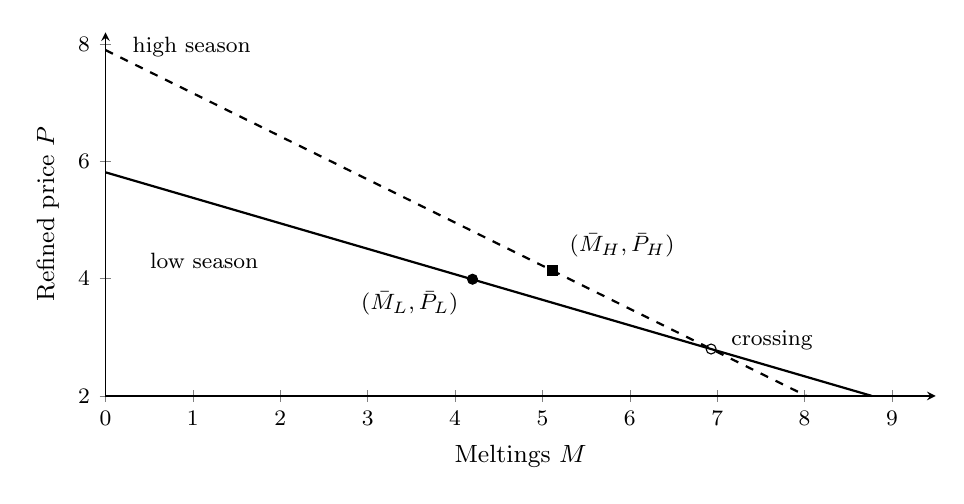
\begin{tikzpicture}
\begin{axis}[
  width=\linewidth, height=6.2cm,
  xmin=0, xmax=9.5, ymin=2, ymax=8.2,
  axis lines=left,
  xlabel={Meltings $M$}, ylabel={Refined price $P$},
  xlabel style={font=\small}, ylabel style={font=\small},
  tick label style={font=\footnotesize},
  clip=false]
\addplot[thick, black, domain=0:8.77, samples=2] {5.813 - x/2.30};
\addplot[thick, black, dashed, domain=0:8.02, samples=2] {7.897 - x/1.36};
\addplot[only marks, mark=*, mark size=1.8pt] coordinates {(4.20,3.99)};
\addplot[only marks, mark=square*, mark size=1.8pt] coordinates {(5.11,4.14)};
\addplot[only marks, mark=o, mark size=1.8pt] coordinates {(6.93,2.80)};
\node[font=\footnotesize, anchor=north west] at (axis cs:0.4,4.6) {low season};
\node[font=\footnotesize, anchor=west] at (axis cs:0.2,7.95) {high season};
\node[font=\footnotesize, anchor=south west] at (axis cs:5.2,4.2) {$(\bar M_H, \bar P_H)$};
\node[font=\footnotesize, anchor=north east] at (axis cs:4.15,3.95) {$(\bar M_L, \bar P_L)$};
\node[font=\footnotesize, anchor=west] at (axis cs:7.05,2.95) {crossing};
\end{axis}
\end{tikzpicture}
\caption{Demand: $M = 13.37 - 2.30P$ (solid) and $M = 10.74 - 1.36P$ (dashed).}
\end{subfigure}\hfill
\begin{subfigure}[t]{0.48\textwidth}
\centering
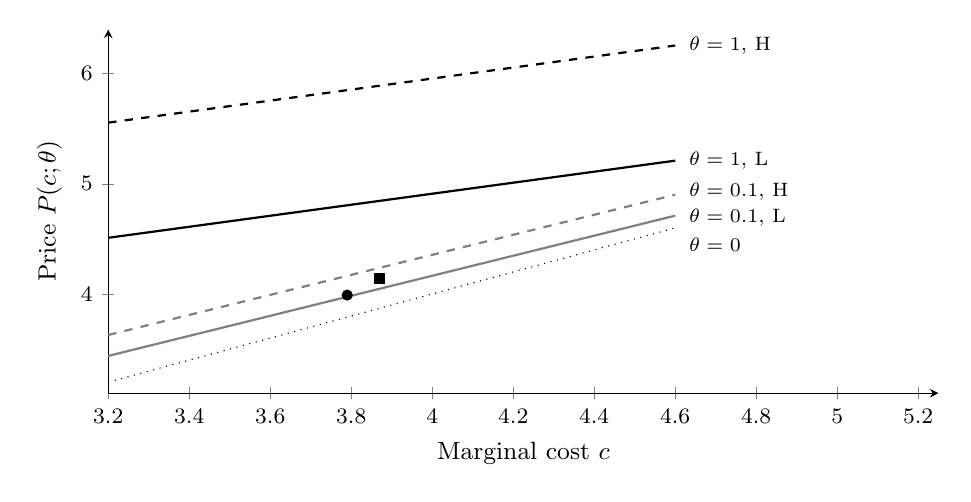
\begin{tikzpicture}
\begin{axis}[
  width=\linewidth, height=6.2cm,
  xmin=3.2, xmax=5.25, ymin=3.1, ymax=6.4,
  axis lines=left,
  xlabel={Marginal cost $c$}, ylabel={Price $P(c;\theta)$},
  xlabel style={font=\small}, ylabel style={font=\small},
  tick label style={font=\footnotesize},
  clip=false]
\addplot[thick, black, domain=3.2:4.6, samples=2] {(5.82 + x)/2};
\addplot[thick, black, dashed, domain=3.2:4.6, samples=2] {(7.91 + x)/2};
\addplot[thick, gray, domain=3.2:4.6, samples=2] {(0.582 + x)/1.1};
\addplot[thick, gray, dashed, domain=3.2:4.6, samples=2] {(0.791 + x)/1.1};
\addplot[thin, black, dotted, domain=3.2:4.6, samples=2] {x};
\addplot[only marks, mark=*, mark size=1.8pt] coordinates {(3.79,3.99)};
\addplot[only marks, mark=square*, mark size=1.8pt] coordinates {(3.87,4.14)};
\node[font=\scriptsize, anchor=west] at (axis cs:4.61,6.255) {$\theta = 1$, H};
\node[font=\scriptsize, anchor=west] at (axis cs:4.61,5.21) {$\theta = 1$, L};
\node[font=\scriptsize, anchor=west] at (axis cs:4.61,4.93) {$\theta = 0.1$, H};
\node[font=\scriptsize, anchor=west] at (axis cs:4.61,4.69) {$\theta = 0.1$, L};
\node[font=\scriptsize, anchor=west] at (axis cs:4.61,4.45) {$\theta = 0$};
\end{axis}
\end{tikzpicture}
\caption{Pricing rules $P(c;\theta) = \frac{\theta\alpha_s + c}{1 + \theta}$, low (solid) and high (dashed)
season.}
\end{subfigure}
\caption{The canning season rotates demand. Panel (a) shows the estimated linear demand curves, which cross at
$P = 2.80$, below all observed prices, and the season means. Panel (b) shows the implied pricing rules with
$\alpha_L = 5.82$ and $\alpha_H = 7.91$ (\cref{tab:03-gm-derived}). The monopoly price rises by
$\frac{\alpha_H - \alpha_L}{2} = 1.05$ in the high season at given cost, while competitive pricing does not
move. The markers are the season means of $(c_t, P_t)$ with $c_t = 0.26 + 1.075\,P^{\mathrm{raw}}_t$.
Constructed from \citet{GenesoveMullin1998}, Tables 2--4.}
\label{fig:03-gm-pricing-rules}
\end{figure}

\subsection{The direct measure of conduct}\label{sec:03-sugar-direct}

With demand in hand, the supply relation \eqref{eq:03-gm-supply} gives a pricing rule for every conduct
parameter.

\begin{proposition}[Pricing rules for the demand family]\label{prop:03-gm-pricing}
Let demand be \eqref{eq:03-gm-demand} and marginal cost $c$ be constant. The price that solves
\eqref{eq:03-gm-supply} is
\begin{equation}\label{eq:03-gm-pricing}
P(c;\theta) = \frac{\theta\alpha + \gamma c}{\gamma + \theta},
\qquad
P^M(c) \equiv P(c;1) = \frac{\alpha + \gamma c}{1 + \gamma}.
\end{equation}
In the log-linear case ($\alpha = 0$, $\gamma = -\varepsilon$) this is
$P(c;\theta) = \frac{\varepsilon}{\varepsilon - \theta}\,c$, and in the exponential limit it is
$P(c;\theta) = c + \frac{\theta}{\lambda}$. Pass-through is $\frac{\partial P}{\partial c} =
\frac{\gamma}{\gamma + \theta}$.
\end{proposition}

\begin{proof}
Since $P'(Q) = \frac{1}{Q'(P)}$, \cref{lem:03-gm-demand}(i) gives
\begin{equation*}
Q\,P'(Q) = \frac{Q(P)}{Q'(P)} = -\frac{\alpha - P}{\gamma}.
\end{equation*}
Substituting into \eqref{eq:03-gm-supply},
\begin{equation*}
P - \frac{\theta(\alpha - P)}{\gamma} = c
\;\Longleftrightarrow\;
\gamma P + \theta P = \gamma c + \theta\alpha
\;\Longleftrightarrow\;
P = \frac{\theta\alpha + \gamma c}{\gamma + \theta}.
\end{equation*}
Setting $\alpha = 0$ and $\gamma = -\varepsilon$ gives $P = \frac{-\varepsilon c}{\theta - \varepsilon} =
\frac{\varepsilon}{\varepsilon - \theta}c$. In the exponential limit, $\frac{\alpha - P}{\gamma} \to
\frac{1}{\lambda}$ by \cref{lem:03-gm-demand}(ii), so the supply relation reads $P - \frac{\theta}{\lambda} =
c$. Differentiating \eqref{eq:03-gm-pricing} in $c$ gives the pass-through.
\end{proof}

The pass-through formula agrees with \cref{prop:03-passthrough}. With flat marginal cost that proposition
gives $\rho = \frac{1}{1 + \theta(1 - \chi)}$, and $\chi = 1 - \frac{1}{\gamma}$ from
\cref{lem:03-gm-demand}(iii) yields $\rho = \frac{1}{1 + \frac{\theta}{\gamma}} = \frac{\gamma}{\gamma +
\theta}$. Two features matter below. The pricing rule is affine in cost with a slope that depends on $\theta$
and $\gamma$ only. Its intercept $\frac{\theta\alpha}{\gamma + \theta}$ moves with the season whenever
$\alpha$ does, and by more the larger is $\theta$. Under exponential demand the slope is one for every
$\theta$, so pass-through carries no information about conduct \citep{BulowPfleiderer1983}.

Monopoly requires an elastic demand at the monopoly price. At $P^M$, $\alpha - P^M = \frac{\gamma(\alpha -
c)}{1 + \gamma}$, so $\varepsilon(P^M) = \frac{\gamma P^M}{\alpha - P^M} = \frac{\alpha + \gamma c}{\alpha -
c}$. For $c > 0$ this exceeds one if and only if $\gamma > -1$ when $\alpha > c$, and $\gamma < -1$ when
$\alpha < c$ (WP p.~24). In the log-linear form, the high-season elasticity of 1.10 barely satisfies this
condition, and the implied monopoly price is enormous.

\Cref{tab:03-gm-derived} reports the implied pricing rules, the elasticities at the full-sample mean, and the
direct conduct measure.

\begin{table}[htbp]
\centering
\caption{Demand for refined sugar: derived estimates and the direct measure of conduct}\label{tab:03-gm-derived}
\small
\begin{tabular}{@{}lccccc@{}}
\toprule
 & (1) Quadratic & (2) Linear & (3) Log-linear & (4) Exponential & (5) Lerner\\
\midrule
$P^M(c)$, low season & $2.57 + 0.67c$ & $2.91 + 0.5c$ & $1.97c$ & $1.89 + c$ & \\
$P^M(c)$, high season & $3.96 + 0.67c$ & $3.96 + 0.5c$ & $10.1c$ & $3.85 + c$ & \\
\addlinespace
$P(c;\theta)$, low season & $\frac{7.72\theta + 2c}{2 + \theta}$ & $\frac{5.82\theta + c}{1 + \theta}$ &
 $\frac{2.03}{2.03 - \theta}c$ & $1.89\theta + c$ & \\[4pt]
$P(c;\theta)$, high season & $\frac{11.88\theta + 2c}{2 + \theta}$ & $\frac{7.91\theta + c}{1 + \theta}$ &
 $\frac{1.10}{1.10 - \theta}c$ & $3.85\theta + c$ & \\
\addlinespace
\multicolumn{6}{@{}l}{\textit{Elasticity $\varepsilon$ at the full-sample mean}}\\
Low season & 2.18 & 2.24 & 2.03 & 2.13 & \\
High season & 1.03 & 1.04 & 1.10 & 1.05 & \\
\addlinespace
\multicolumn{5}{@{}l}{\textit{Adjusted Lerner index $L_\varepsilon$}} & \textit{Unadjusted}\\
Mean & 0.099 & 0.107 & 0.095 & 0.097 & 0.054\\
Standard deviation & 0.097 & 0.118 & 0.083 & 0.089 & 0.045\\
Standard error & 0.024 & 0.028 & 0.021 & 0.022 & 0.0046\\
\bottomrule
\end{tabular}

\smallskip
\begin{minipage}{0.92\textwidth}\footnotesize
Notes: Reproduced from \citet{GenesoveMullin1998}, Table 4, which combines WP Tables 7 and 8. $L_\varepsilon =
\varepsilon\,\frac{P - c}{P}$ with $c = 0.26 + 1.075\,P^{\mathrm{raw}}$, computed quarter by quarter. The
standard errors account for the estimation of demand (WP Table 8, column 4). Standard errors that ignore it
are 0.010, 0.012, 0.008 and 0.009 (WP Table 8, column 3). WP Table 7 prints $7.88\theta$ in the high-season
linear rule.
\end{minipage}
\end{table}

\casehead{Checking the derived estimates}
Every entry follows from \cref{tab:03-gm-demand} and \cref{prop:03-gm-pricing}. In the quadratic form,
$P^M = \frac{7.72}{3} + \frac{2}{3}c = 2.57 + 0.67c$, and the high-season intercept is $\frac{11.88}{3} =
3.96$. In the linear form the choke prices are $\alpha_L = \frac{13.37}{2.30} = 5.81$ and $\alpha_H =
\frac{10.74}{1.36} = 7.90$, so $P^M = \frac{\alpha_s}{2} + \frac{c}{2}$ has intercepts 2.91 and 3.95. The
printed 5.82, 7.91 and 3.96 reflect unrounded coefficients. In the exponential form, $\frac{1}{0.53} = 1.89$
and $\frac{1}{0.26} = 3.85$. In the log-linear form, the monopoly markup factor
$\frac{\varepsilon}{\varepsilon - 1}$ equals $\frac{2.03}{1.03} = 1.97$ in the low season. In the high
season it equals $\frac{1.10}{0.10} = 11.0$ at $\varepsilon_H = 1.10$. The printed 10.1 corresponds to
$\varepsilon_H = \frac{10.1}{9.1} = 1.11$. Rounding cannot reconcile the two. Every elasticity in $[1.095,
1.105)$, which rounds to 1.10, gives a factor between 10.52 and 11.53. The published table is thus inconsistent
with its own elasticity, and the source does not explain why. The digits of 11.0 may have been transposed. We
reproduce the printed 10.1, which gives the high-season monopoly price of about 39 below. The factor 11.0 would
give about 43. The elasticities at $\bar P = 4.03$ follow from \cref{lem:03-gm-demand}(i). For example,
$\frac{2 \times 4.03}{7.72 - 4.03} = 2.18$ and $\frac{2 \times 4.03}{11.88 - 4.03} = 1.03$ for the quadratic,
$0.53 \times 4.03 = 2.14$ (2.13 in the table, from unrounded coefficients) and $0.26 \times 4.03 = 1.05$ for the
exponential.

\casehead{Observed prices are far below monopoly}
At the low-season means, marginal cost is $c = 0.26 + 1.075 \times 3.28 = 3.79$. The linear monopoly price
is then $2.91 + 0.5 \times 3.79 = 4.80$, against an observed mean of 3.99. In the high season, $c = 0.26 +
1.075 \times 3.36 = 3.87$ and $P^M = 3.96 + 0.5 \times 3.87 = 5.90$, against 4.14. The quadratic form puts
the monopoly prices at 5.10 and 6.54, the exponential form at 5.68 and 7.72, and the log-linear form at 7.47
and about 39. Whatever the demand form, the industry priced far below the monopoly level (WP p.~27). Panel (b) of
\cref{fig:03-gm-pricing-rules} shows the gap.

\casehead{The direct measure}
The first estimation method uses everything. Marginal cost is \eqref{eq:03-gm-direct-cost}, the elasticity
comes from the season's demand curve evaluated at the quarter's price, and conduct is computed quarter by
quarter:
\begin{equation}\label{eq:03-gm-direct}
L_{\varepsilon t} = \varepsilon_{s(t)}(P_t)\,\frac{P_t - c_t}{P_t} = \frac{P_t - c_t}{m_t},
\qquad m_t = \frac{\alpha_{s(t)} - P_t}{\gamma_{s(t)}} .
\end{equation}
The second expression uses \cref{lem:03-gm-demand}(i): conduct is the price-cost margin divided by the
markup term $m_t = \frac{Q_t}{\lvert Q'(P_t)\rvert}$ of \cref{sec:03-corts}. The direct measure is a
function of data and of the estimated demand parameters. Its standard error must reflect the second source
of noise. Genesove and Mullin stack the demand moment conditions with the moment
$\frac{1}{n}\sum_t \left(L_{\varepsilon t} - \bar L_\varepsilon\right) = 0$ and compute the usual GMM
variance for the mean $\bar L_\varepsilon$ (WP p.~31, fn.~45). Accounting for estimated demand more than
doubles the standard errors.

\casehead{Results}
The mean adjusted Lerner index lies between 0.095 and 0.107 across the four demand forms
(\cref{tab:03-gm-derived}). Genesove and Mullin take $\theta = 0.10$ as their direct measure. This is the
conduct of a static symmetric Cournot oligopoly with ten firms. Both perfect competition and monopoly are
rejected: the mean is about four standard errors above zero and far below one. The unadjusted Lerner index
of 0.054 says that price exceeded marginal cost by only 5 percent. With demand elasticities near two, even
this small margin corresponds to a conduct parameter of 0.10. With the lower bound $c_0 = 0.16$, the mean index
rises to 0.14 (log-linear and exponential), 0.15 (quadratic) and 0.16 (linear). The value $0.15$ corresponds
to a symmetric Cournot oligopoly with about seven firms, so the conclusions do not change (WP p.~37).

\begin{figure}[!htb]
\centering
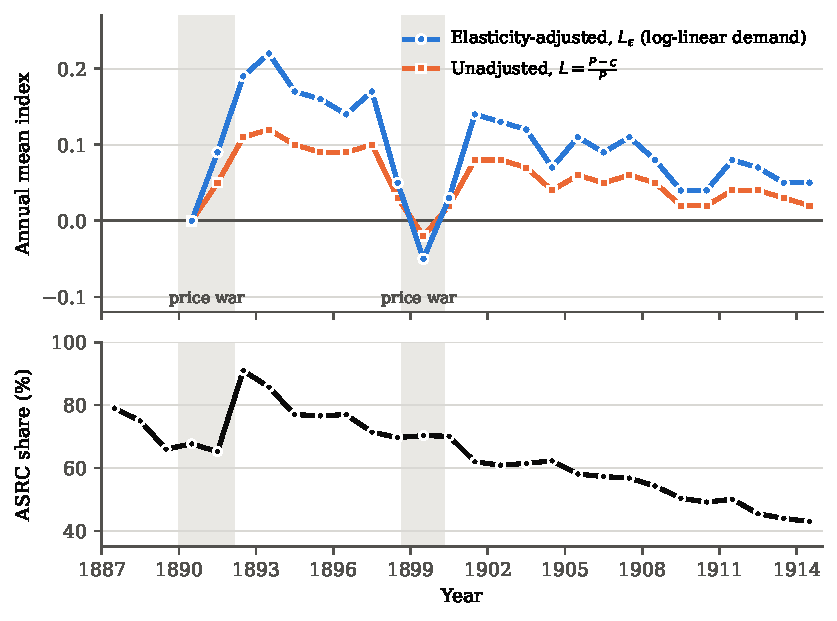
\includegraphics[width=0.86\textwidth]{figures/ch03/gm_lerner_time.pdf}
\caption{Annual means of the unadjusted Lerner index $\frac{P - c}{P}$ and of the elasticity-adjusted index
$L_\varepsilon$ (log-linear demand), top, and the market share of the American Sugar Refining Company,
bottom. Shaded bands mark the two post-entry price wars (January 1890 to February 1892 and September 1898 to
April 1900). Redrawn from \citet{GenesoveMullin1995}, WP Table 9.}
\label{fig:03-gm-lerner-time}
\end{figure}

\casehead{Conduct over time}
\Cref{fig:03-gm-lerner-time} plots the annual means of WP Table 9. Conduct follows structure. The adjusted
index is zero in 1890 during the Spreckels war. It rises to between 0.14 and 0.22 in 1892--1897, after ASRC
had consolidated 91 percent of the market. It collapses again in the Arbuckle war, to $-0.05$ in 1899,
which means pricing below the measured marginal cost. Willett and Gray themselves reported in October 1898
that refiners were selling at ``an actual loss'' (WP p.~33, fn.~47). After 1900 the index drifts down from
0.14 to about 0.05 as ASRC's share falls toward 43 percent. Across the twenty years outside the price wars (excluding 1890, 1891 and 1898--1900),
the correlation between the annual adjusted index and ASRC's share is 0.92 (our computation from WP Table 9).
The averages over 1890--1914 are 0.09 for the adjusted index, 0.05 for the unadjusted index and 63.1 percent
for ASRC's share.

\begin{table}[htbp]
\centering
\caption{Seasonality of the direct conduct measure}\label{tab:03-gm-seasonality}
\small
\begin{tabular}{@{}lcccccccc@{}}
\toprule
 & \multicolumn{2}{c}{Quarter I} & \multicolumn{2}{c}{Quarter II} & \multicolumn{2}{c}{Quarter III (high)} &
 \multicolumn{2}{c}{Quarter IV}\\
\cmidrule(lr){2-3}\cmidrule(lr){4-5}\cmidrule(lr){6-7}\cmidrule(l){8-9}
 & Mean & S.D. & Mean & S.D. & Mean & S.D. & Mean & S.D.\\
\midrule
Unadjusted $L$ & 0.048 & 0.042 & 0.065 & 0.042 & 0.064 & 0.047 & 0.038 & 0.047\\
$L_\varepsilon$, quadratic & 0.096 & 0.091 & 0.142 & 0.104 & 0.071 & 0.057 & 0.083 & 0.117\\
$L_\varepsilon$, linear & 0.102 & 0.106 & 0.162 & 0.138 & 0.075 & 0.063 & 0.086 & 0.134\\
$L_\varepsilon$, log-linear & 0.097 & 0.085 & 0.132 & 0.085 & 0.071 & 0.051 & 0.078 & 0.096\\
$L_\varepsilon$, exponential & 0.097 & 0.087 & 0.136 & 0.092 & 0.071 & 0.055 & 0.081 & 0.106\\
\bottomrule
\end{tabular}

\smallskip
\begin{minipage}{0.92\textwidth}\footnotesize
Notes: Reproduced from \citet{GenesoveMullin1995}, WP Table 10. Means and standard deviations across
quarters of the same type.
\end{minipage}
\end{table}

\casehead{Conduct over the year}
\Cref{tab:03-gm-seasonality} shows that conduct also varies within the year. It is least competitive in the
second quarter and most competitive in the third, the high season. This pattern fits dynamic oligopoly models
in which the expectation of better demand ahead helps collusion and the expectation of worse demand harms it
\citep{RotembergSaloner1986,HaltiwangerHarrington1991}. Genesove and Mullin note a caveat. The unadjusted
index is equal in the second and third quarters, so the pattern may be an artifact of attaching the
inelastic high-season demand to the third quarter alone (WP pp.~33--34). Either way, conduct that varies
systematically with a demand shifter contradicts the assumption of the NEIO method that $\theta$ is
uncorrelated with the instruments. Genesove and Mullin argue that the proper test of a method is its success in
doing what it is meant to do, whatever the truth of its assumptions (WP p.~34). The next subsection shows that this
seasonal pattern explains much of what the NEIO estimator finds.

The low level of the index, relative to the industry's concentration, has a natural explanation. Pricing was
constrained by the threat of domestic entry and of foreign imports (WP p.~34). The price wars of 1890 and
1898--1900 show that the entry threat was not idle.

\subsection{Estimating conduct with cost treated as unknown}\label{sec:03-sugar-neio}

We now put ourselves in the position of an NEIO researcher who observes prices, quantities, the raw sugar
price and the instruments, but does not know $c_0$, $k$ or both.

\casehead{The pricing equation}
Substituting \eqref{eq:03-gm-cost} into \eqref{eq:03-gm-pricing} gives the reduced-form pricing equation
(WP eq.~12)
\begin{equation}\label{eq:03-gm-reduced}
P_t = \frac{\alpha_{s}\theta + c_0\gamma_{s}}{\gamma_{s} + \theta}
 + \frac{\gamma_{s}}{\gamma_{s} + \theta}\,k\,P^{\mathrm{raw}}_t + u_t ,
\qquad s = s(t),
\end{equation}
where $u_t$ is a pricing error from unobserved cost or conduct shocks. In the exponential case the equation
is $P_t = \frac{\theta}{\lambda_s} + c_0 + kP^{\mathrm{raw}}_t + u_t$ (WP p.~34, fn.~49). Multiplying
\eqref{eq:03-gm-reduced} by $\gamma_s + \theta$ gives the moment condition that Genesove and Mullin estimate
(WP eq.~13):
\begin{equation}\label{eq:03-gm-moment}
\E\Big[\big\{(\gamma_s + \theta)P_t - \alpha_s\theta - c_0\gamma_s - \gamma_s k P^{\mathrm{raw}}_t\big\}\,z_t\Big]
= 0 .
\end{equation}
The demand parameters $(\alpha_s, \gamma_s)$ are fixed at their estimates in \cref{tab:03-gm-demand}. The
unknowns are $\theta$ and whichever cost parameters the researcher does not know.

The raw price must be instrumented. Whether $u_t$ is a cost shock or a conduct shock, a positive $u_t$ raises
the refined price and lowers the quantity of refined sugar demanded. Refiners then demand less raw sugar,
which lowers the raw price. The pricing error is therefore negatively correlated with $P^{\mathrm{raw}}_t$ (WP
p.~34). Log Cuban imports again serve as the excluded cost shifter.

\casehead{The information hierarchy}
Genesove and Mullin organize the comparison by what the researcher knows about cost (WP p.~35).
\begin{enumerate}[label=(\Roman*)]
\item Neither $c_0$ nor $k$ is known. The unknowns are $(\theta, c_0, k)$, and the instruments are
$z_t = (1, H_t, \ln\mathit{CUBA}_t)$.
\item The input coefficient $k = 1.075$ is known, and $c_0$ is not. The unknowns are $(\theta, c_0)$, and the
instruments are $z_t = (1, H_t)$. This is the position of the cigarette studies of \citet{Sumner1981},
\citet{Sullivan1985} and \citet{AshenfelterSullivan1987} (\cref{sec:03-sumner}). In those studies an excise
tax enters marginal cost with a known coefficient of one.
\item Both $c_0 = 0.26$ and $k = 1.075$ are known. Then $\theta$ is observed directly, as in
\eqref{eq:03-gm-direct}.
\end{enumerate}
The fourth combination, $c_0$ known and $k$ unknown, is implausible in this industry and is not explored. In
both (I) and (II) the number of instruments equals the number of unknowns, so the nonlinear instrumental
variables (NLIV) estimator solves the sample analogue of \eqref{eq:03-gm-moment} exactly. Estimating demand
first and the pricing equation second is the two-step method. Stacking the demand moments and
\eqref{eq:03-gm-moment} in a single GMM problem is the joint version of the same estimator.

\casehead{Standard errors with estimated demand}
The two-step estimator inherits the noise in the demand estimates. Let $b = (\theta, c_0, k)^\T$, let $a$ be
the demand parameters with $\sqrt{n}(\hat a - a_0) \to N(0, W_1)$, and let $\bar g_n(b, a)$ be the sample
analogue of \eqref{eq:03-gm-moment}. A mean-value expansion of $\bar g_n(\hat b, \hat a) = 0$ around
$(b_0, a_0)$ gives
\begin{equation*}
0 = \bar g_n(b_0, a_0) + D\,(\hat b - b_0) + C\,(\hat a - a_0) + o_p\!\left(n^{-\frac{1}{2}}\right),
\qquad D = \E\left[\frac{\partial g}{\partial b^\T}\right],\;\; C = \E\left[\frac{\partial g}{\partial a^\T}\right].
\end{equation*}
Solving for $\hat b - b_0$,
\begin{equation*}
\sqrt{n}\,(\hat b - b_0) = -D^{-1}\sqrt{n}\,\bar g_n(b_0, a_0) - D^{-1}C\,\sqrt{n}\,(\hat a - a_0) + o_p(1).
\end{equation*}
If the pricing moments and the demand estimates are asymptotically uncorrelated, the asymptotic variance is
\begin{equation}\label{eq:03-gm-variance}
\operatorname{Avar}(\hat b) = W_2 + D^{-1} C\, W_1\, C^\T \left(D^{-1}\right)^\T,
\qquad W_2 = D^{-1} S \left(D^{-1}\right)^\T ,
\end{equation}
where $S$ is the long-run variance of the pricing moments. Genesove and Mullin estimate $S$ and $W_1$ by
Newey-West with four lags (WP p.~36). The zero-correlation assumption fits their interpretation: demand errors
are proportional shifts that do not move the pricing rule. Without it, the joint GMM estimator delivers
correct standard errors directly (\cref{app:econometrics}).

\begin{table}[htbp]
\centering
\caption{NLIV estimates of conduct and cost parameters}\label{tab:03-gm-nliv}
\small
\setlength{\tabcolsep}{4.5pt}
\begin{tabular}{@{}lccccccccc@{}}
\toprule
 & \multicolumn{2}{c}{Quadratic} & \multicolumn{2}{c}{Linear} & \multicolumn{2}{c}{Log-linear} &
 \multicolumn{2}{c}{Exponential} & Direct\\
\cmidrule(lr){2-3}\cmidrule(lr){4-5}\cmidrule(lr){6-7}\cmidrule(lr){8-9}\cmidrule(l){10-10}
 & (1) & (2) & (3) & (4) & (5) & (6) & (7) & (8) & (9)\\
\midrule
$\hat\theta$ & 0.037 & 0.035 & 0.038 & 0.037 & 0.045 & 0.040 & 0.041 & 0.037 & 0.10\\
 & (0.024) & (0.024) & (0.024) & (0.024) & (0.028) & (0.026) & (0.026) & (0.025) & \\
$\hat c_0$ & 0.529 & 0.393 & 0.465 & 0.39 & 0.760 & 0.381 & 0.700 & 0.389 & 0.26\\
 & (0.272) & (0.062) & (0.285) & (0.061) & (0.262) & (0.070) & (0.279) & (0.065) & \\
$\hat k$ & 1.033 & & 1.052 & & 0.956 & & 0.978 & & 1.075\\
 & (0.082) & & (0.085) & & (0.081) & & (0.083) & & \\
\bottomrule
\end{tabular}

\smallskip
\begin{minipage}{0.92\textwidth}\footnotesize
Notes: Reproduced from \citet{GenesoveMullin1995}, WP Table 11. Columns (1), (3), (5) and (7) estimate
$(\theta, c_0, k)$ with instruments $(1, H_t, \ln\mathit{CUBA}_t)$. Columns (2), (4), (6) and (8) impose $k =
1.075$ and use $(1, H_t)$. Demand parameters from \cref{tab:03-gm-demand}. Newey-West standard errors (four
lags), corrected for estimated demand, in parentheses. Column (9) is the direct measure. $N = 97$.
\end{minipage}
\end{table}

\casehead{Results}
\Cref{tab:03-gm-nliv} reports the estimates. Genesove and Mullin draw four conclusions (WP pp.~36--37).
First, the NLIV estimate of $\theta$ is close to the direct measure. It lies between 0.035 and 0.045 in all
eight specifications. Monopoly is rejected everywhere, as is any $\theta$ above 0.11. Perfect competition
cannot be rejected: the $t$ ratios are between 1.46 and 1.61. The estimates are below the direct measure in
every case. The upper limits of the 95 percent confidence intervals run from 0.082 to 0.100 (our computation),
so the direct value of 0.10 sits at or just beyond their edge. Second, the estimates are robust to the form
of demand. This answers the common complaint that conduct estimates hinge on functional form. Third, the cost
parameters are recovered less well. The coefficient $k$ is underestimated in all four forms, although
$k = 1.075$ is never rejected. The parameter $c_0$ is overestimated, by 50 cents in the log-linear case (0.760
against 0.26). Fourth, knowing $k$ hardly changes $\hat\theta$. It sharpens the estimate of $c_0$, which falls to
0.38--0.39 with standard errors near 0.06. Because $c_0$ does not enter the NLIV estimator, setting $c_0 =
0.16$ leaves \cref{tab:03-gm-nliv} unchanged and moves only the benchmark, from 0.10 to about 0.15.

\casehead{What identifies $\theta$: the seasonal shift}
Why does the method deliver 0.04? In the quadratic, linear and exponential forms only the intercept of
\eqref{eq:03-gm-reduced} differs across seasons. The equation can then be written as a linear regression,
\begin{equation}\label{eq:03-gm-linear-rf}
P_t = \pi_0 + \pi_1 H_t + \pi_2 P^{\mathrm{raw}}_t + u_t .
\end{equation}
For the linear and quadratic forms, with $\gamma$ common to both seasons,
\begin{equation*}
\pi_0 = \frac{\theta\alpha_L + \gamma c_0}{\gamma + \theta},
\qquad
\pi_1 = \frac{\theta\,(\alpha_H - \alpha_L)}{\gamma + \theta},
\qquad
\pi_2 = \frac{\gamma k}{\gamma + \theta}.
\end{equation*}
For the exponential form, $\pi_0 = \frac{\theta}{\lambda_L} + c_0$, $\pi_1 = \theta\left(\frac{1}{\lambda_H} -
\frac{1}{\lambda_L}\right)$ and $\pi_2 = k$. In each case the map from $(\theta, c_0, k)$ to $(\pi_0, \pi_1,
\pi_2)$ is one to one. For the linear and quadratic forms, inverting it gives
\begin{equation}\label{eq:03-gm-inversion}
\theta = \frac{\gamma\,\pi_1}{(\alpha_H - \alpha_L) - \pi_1},
\qquad
k = \frac{\gamma + \theta}{\gamma}\,\pi_2,
\qquad
c_0 = \frac{(\gamma + \theta)\pi_0 - \theta\alpha_L}{\gamma}.
\end{equation}
The conduct parameter is identified only through $\pi_1$, the seasonal shift of the pricing rule at a given
raw price. If the season changed only the scale $\beta$, so that $\alpha_H = \alpha_L$, then $\pi_1 = 0$ for
every $\theta$ and conduct would not be identified. A seasonal change in $\alpha$ suffices, even a parallel
shift of linear demand. Identification therefore rests on the restriction that marginal cost is constant in
output (\cref{sec:03-other-routes}). The general rotation argument of \cref{prop:03-rotation,prop:03-lau} is
needed only when the slope of marginal cost is unknown. At $\theta = 1$,
$\pi_1$ equals the seasonal shift of the monopoly price, $\frac{\alpha_H - \alpha_L}{1 + \gamma}$. The
estimator thus compares the observed seasonal price shift with the shift that a monopolist would make.

\begin{table}[htbp]
\centering
\caption{Linear pricing equations for refined sugar}\label{tab:03-gm-reduced}
\small
\begin{tabular}{@{}lcccccc@{}}
\toprule
 & (1) & (2) & (3) & (4) & (5) & (6)\\
 & IV & IV & IV & OLS & OLS & OLS\\
\midrule
Raw price & 1.02 & 0.93 & 1.01 & 0.99 & 0.98 & 0.99\\
 & (0.09) & (0.09) & (0.08) & (0.05) & (0.05) & (0.05)\\
High season $\times$ raw price & & 0.31 & & & 0.04 & \\
 & & (0.11) & & & (0.07) & \\
High season & & $-0.97$ & 0.08 & & $-0.07$ & 0.08\\
 & & (0.38) & (0.03) & & (0.22) & (0.03)\\
Constant & 0.67 & 0.94 & 0.66 & 0.75 & 0.77 & 0.74\\
 & (0.28) & (0.28) & (0.26) & (0.16) & (0.16) & (0.16)\\
$\chi^2_{(2)}$ test & & 21.67 & & & 6.66 & \\
\bottomrule
\end{tabular}

\smallskip
\begin{minipage}{0.92\textwidth}\footnotesize
Notes: Reproduced from \citet{GenesoveMullin1995}, WP Table 12. Dependent variable: refined price, $N = 97$.
Instruments in columns (1) and (2): high season, log Cuban imports and their interaction. The $\chi^2_{(2)}$
statistic tests that the coefficients on high season and its interaction with the raw price are both zero.
\end{minipage}
\end{table}

Column (3) of \cref{tab:03-gm-reduced} estimates \eqref{eq:03-gm-linear-rf} by instrumental variables. The
refined price rises by only 8 cents in the high season at a given raw price. The demand estimates imply
much larger shifts of the monopoly price: $\frac{\alpha_H - \alpha_L}{2} = 1.05$ for linear demand and
$\frac{1}{\lambda_H} - \frac{1}{\lambda_L} = 3.85 - 1.89 = 1.96$ for exponential demand. Under exponential
demand the intercept is $\frac{\theta}{\lambda_s} + c_0$, so
\begin{equation*}
\hat\theta \approx \frac{0.08}{1.96} \approx 0.04
\end{equation*}
(WP p.~38). Under linear demand, \eqref{eq:03-gm-inversion} with $\gamma = 1$ and $\alpha_H - \alpha_L =
7.91 - 5.82 = 2.09$ gives
\begin{equation*}
\theta = \frac{0.08}{2.09 - 0.08} = 0.040,
\quad
k = 1.040 \times 1.01 = 1.050,
\quad
c_0 = 1.040 \times 0.66 - 0.040 \times 5.82 = 0.455 .
\end{equation*}
These reproduce column (3) of \cref{tab:03-gm-nliv}, $(0.038, 0.465, 1.052)$, up to rounding. The quadratic form
gives $(0.039, 0.52, 1.03)$ against $(0.037, 0.529, 1.033)$. The same arithmetic explains the cost
estimates. The raw-price coefficient of 1.01 forces $k$ below 1.075, because the slope $\frac{\gamma
k}{\gamma + \theta}$ is close to $k$ when $\theta$ is small. With $\theta$ understated, $c_0$ must absorb
the remaining margin between the refined and raw prices, so $c_0$ is overstated (WP p.~38).

\casehead{A closed form when $k$ is known}
When $k$ is known, the estimator has an explicit form that links it to the direct measure. Divide the
expression in braces in \eqref{eq:03-gm-moment} by $\gamma_s$ and use \cref{lem:03-gm-demand}(i):
\begin{equation*}
\frac{(\gamma_s + \theta)P_t - \alpha_s\theta - c_0\gamma_s - \gamma_s k P^{\mathrm{raw}}_t}{\gamma_s}
= \big(P_t - kP^{\mathrm{raw}}_t\big) - c_0 - \theta\,\frac{\alpha_s - P_t}{\gamma_s}
= G_t - c_0 - \theta\, m_t .
\end{equation*}
The pricing equation thus says that the proper margin equals non-sugar cost plus conduct times the markup
term. This holds in all four forms, and in the exponential form $m_t = \frac{1}{\lambda_s}$.

\begin{proposition}[The NLIV estimator with known $k$]\label{prop:03-gm-wald}
Suppose $k$ is known, the instruments are $(1, H_t)$, and demand is quadratic, linear or exponential. Let $\bar G_s$ and $\bar m_s$ be the season means of the proper
margin and of the markup term. Then
\begin{equation}\label{eq:03-gm-wald}
\hat\theta = \frac{\bar G_H - \bar G_L}{\bar m_H - \bar m_L},
\qquad
\hat c_0 = \bar G_L - \hat\theta\,\bar m_L .
\end{equation}
If the true marginal cost is \eqref{eq:03-gm-cost} and $\theta_t$ denotes true conduct, then
\begin{equation}\label{eq:03-gm-corts}
\hat\theta = \frac{\overline{(\theta m)}_H - \overline{(\theta m)}_L}{\bar m_H - \bar m_L},
\end{equation}
where $\overline{(\theta m)}_s$ is the season mean of $\theta_t m_t$.
\end{proposition}

\begin{proof}
In the quadratic and linear forms $\gamma$ is common to both seasons, so multiplying each moment by the
constant $\frac{1}{\gamma}$ does not change the solution. In the exponential form the moment is
$G_t - c_0 - \theta m_t$ to begin with. The sample moments with instruments $1$ and $H_t$ are
$\sum_t (G_t - c_0 - \theta m_t) = 0$ and $\sum_t H_t(G_t - c_0 - \theta m_t) = 0$. Their difference is the
sum over low-season quarters, so the two conditions are equivalent to
$\bar G_s = c_0 + \theta\,\bar m_s$ for $s = L, H$. Subtracting the low-season equation from the high-season
equation gives $\hat\theta$, and the low-season equation then gives $\hat c_0$. For the second part, the
definition of true conduct in \eqref{eq:03-gm-direct} gives $P_t - c_t = \theta_t m_t$, so $G_t = c_0 +
\theta_t m_t$ by \eqref{eq:03-gm-proper-margin}. Taking season means and substituting into
\eqref{eq:03-gm-wald} gives \eqref{eq:03-gm-corts}.
\end{proof}

The estimator is a Wald ratio. It divides the seasonal change in the proper margin by the seasonal change in
the markup term predicted by demand. With the published season means, $\bar G_H - \bar G_L = 0.53 - 0.46 =
0.07$ (\cref{tab:03-gm-stats}). In the linear form, $\bar m_s = \alpha_s - \bar P_s$, so $\bar m_H - \bar m_L
= 2.09 - 0.15 = 1.94$. In the exponential form, $\bar m_H - \bar m_L = 1.96$. Hence
\begin{align*}
\text{linear:}\quad & \hat\theta = \frac{0.07}{1.94} = 0.036, &
\hat c_0 &= 0.46 - 0.036 \times 1.83 = 0.39,\\
\text{exponential:}\quad & \hat\theta = \frac{0.07}{1.96} = 0.036, &
\hat c_0 &= 0.46 - 0.036 \times 1.89 = 0.39 .
\end{align*}
Columns (4) and (8) of \cref{tab:03-gm-nliv} report $(0.037, 0.39)$ and $(0.037, 0.389)$. The rounding of the
season means to two decimals limits the precision of this check to about $\pm 0.005$ in $\hat\theta$. The
formula also explains the robustness across forms. Each form predicts nearly the same seasonal change in
the markup term at observed prices, between 1.8 dollars (log-linear, $\frac{4.14}{1.10} - \frac{3.99}{2.03}$
at the season means) and 2.0 dollars (quadratic). The four forms differ greatly far from the
data, as their monopoly prices show, but they agree near it.

\casehead{The Corts critique in the sugar data}
Equation \eqref{eq:03-gm-corts} is the IV estimand of \cref{prop:03-corts} with the season indicator as the
instrument. It equals average conduct only if conduct does not differ between seasons. In the exponential
form the markup term is constant within a season, $m_t = \frac{1}{\lambda_s}$. Writing $\bar\theta_s$ for the
season mean of the direct measure, \eqref{eq:03-gm-corts} becomes
\begin{equation*}
\hat\theta
= \frac{\frac{\bar\theta_H}{\lambda_H} - \frac{\bar\theta_L}{\lambda_L}}{\frac{1}{\lambda_H} - \frac{1}{\lambda_L}}
= \frac{3.85\,\bar\theta_H - 1.89\,\bar\theta_L}{1.96}
= \bar\theta_H - 0.96\,\big(\bar\theta_L - \bar\theta_H\big).
\end{equation*}
\Cref{tab:03-gm-seasonality} gives $\bar\theta_H = 0.071$ for the exponential form. The low-season quarters
average about 0.105, weighting quarters I, II and IV by their numbers of observations. Then $\hat\theta = 0.071 - 0.96 \times 0.034 = 0.038$, essentially the reported
0.037. Implied non-sugar cost is $0.26 + (0.105 - 0.038) \times 1.89 = 0.39$, the reported 0.389. The
NLIV estimate lies below even the high-season conduct, because conduct is lower exactly when the rotator is
on. If conduct had stayed at its mean of about 0.10 throughout, the proper margin would have risen by
$0.10 \times 1.96 = 0.20$ in the high season. It rose by 0.07. The understatement of $\theta$ and the
overstatement of $c_0$ both reflect the mechanism of \citet{Corts1999}. The estimator measures the response of
the margin to the rotation, and here that response understates the level of conduct.\footnote{This decomposition is ours. Genesove and Mullin
report the seasonal pattern and the NLIV estimates separately, and attribute the pattern to dynamic
oligopoly (WP pp.~33--34).}

\casehead{The log-linear form}
Under log-linear demand the slope of the pricing rule, $\frac{\varepsilon_s}{\varepsilon_s - \theta}k$,
differs by season, so the linear reparameterization needs an interaction, column (2) of
\cref{tab:03-gm-reduced}. The lower high-season elasticity predicts a steeper pricing rule in the high
season, and the interaction is positive and significant (0.31). The intercept $\frac{\varepsilon_s c_0}
{\varepsilon_s - \theta}$ should also be higher in the high season, yet the high-season coefficient is
$-0.97$. Using the slopes alone gives $\theta = 0.46$. With $r = \frac{0.93 + 0.31}{0.93}$ the ratio of the
slopes, the condition $\frac{\varepsilon_H(\varepsilon_L - \theta)}{\varepsilon_L(\varepsilon_H - \theta)} = r$
solves for $\theta = 0.463$. Using the intercepts alone gives the nonsensical 2.09 (WP p.~39). The NLIV
estimator forces the ratio of intercept to slope to be the same in both seasons, $\frac{c_0}{k}$, and so
returns estimates close to the other forms. Its implied pricing rules are $P = 0.777 + 0.978\,P^{\mathrm{raw}}$
in the low season and $P = 0.792 + 0.997\,P^{\mathrm{raw}}$ in the high season (our computation from column
(5)).\footnote{WP p.~39, fn.~52, prints $0.793 + 0.997\,P^{\mathrm{raw}}$ for the low season and $0.777 + 0.977\,
P^{\mathrm{raw}}$ for the high season. The factor $\frac{\varepsilon_s}{\varepsilon_s - \theta}$ is larger for the
smaller high-season elasticity, so the steeper rule must belong to the high season. The labels in the footnote
appear to be interchanged.} None of the four forms is consistent with the unrestricted estimates of column (2)
(WP p.~39). The other three forms require equal slopes in the two seasons, a single restriction on the
interaction. Its $t$ ratio is $\frac{0.31}{0.11} = 2.8$, a Wald statistic of about 7.9, so equal slopes are
rejected at the 1 percent level. The $\chi^2_{(2)}$ statistic of 21.67 tests a different hypothesis, that
the seasonal intercept and the interaction are both zero. Genesove and Mullin describe the low-season slope of
0.93 as significantly below 1.075, which would contradict log-linear demand, under which price rises more than
one for one with cost. Its $t$ ratio is only $\frac{1.075 - 0.93}{0.09} = 1.61$. The gap is significant at
the one-sided 10 percent level, and not at the one-sided 5 percent level or at any conventional two-sided level.

\casehead{Ignoring the seasons}
Column (1) of \cref{tab:03-gm-reduced} drops all seasonal effects, as a researcher would who used the known
$k$ but ignored the rotation. The only remaining information on conduct is the slope of the pricing rule,
$\frac{\gamma k}{\gamma + \theta} = 1.02$. Solving,
\begin{equation*}
\theta = \gamma\left(\frac{1.075}{1.02} - 1\right) = 0.054\,\gamma .
\end{equation*}
The implied conduct is proportional to the assumed curvature. It equals 0.054 for linear demand and 0.108 for
quadratic demand (WP p.~39). Quadratic demand without seasons has choke price $\hat\alpha = 8.63$ (standard
error 1.17), and it also gives an excellent estimate of non-sugar cost, $\hat c_0 = 0.23$.\footnote{WP p.~39
prints the fitted curve as $\ln M = 7.37 + 2\ln(8.63 - P)$, with standard errors 0.50 and 1.17. The working
paper measures meltings in hundreds of thousands of long tons (WP p.~26), as in \cref{tab:03-gm-stats}. In
those units the printed intercept predicts meltings of about 34{,}000 at $P = 4$, against a sample mean of
4.43. The source does not say whether the intercept is a misprint or uses another unit. Only the choke price
enters the pricing equation, since $m_t = \frac{\alpha - P_t}{2}$.} The researcher
would have no way to know which answer is right. This is the curvature critique of pass-through tests in
\cref{sec:03-sumner} in another guise: the slope identifies conduct only given $\gamma$. With exponential
demand the slope is $k$ for every $\theta$, and $\theta$ and $c_0$ are not even separately identified
\citep{BulowPfleiderer1983}.

\begin{table}[htbp]
\centering
\caption{Cost estimates and predicted price changes under imposed behavioral models}\label{tab:03-gm-behavioral}
\small
\setlength{\tabcolsep}{4.2pt}
\begin{tabular}{@{}lccccccccc@{}}
\toprule
 & \multicolumn{2}{c}{Competition} & \multicolumn{2}{c}{Cournot I} & \multicolumn{2}{c}{Cournot II} &
 \multicolumn{2}{c}{Monopoly} & Direct\\
\cmidrule(lr){2-3}\cmidrule(lr){4-5}\cmidrule(lr){6-7}\cmidrule(lr){8-9}\cmidrule(l){10-10}
 & (1) & (2) & (3) & (4) & (5) & (6) & (7) & (8) & (9)\\
\midrule
$\hat c_0$ & 0.674 & 0.476 & 0.00 & 0.069 & 0.00 & 0.00 & 0.00 & 0.00 & 0.26\\
 & (0.281) & (0.034) & (0.239) & (0.071) & (0.922) & (0.400) & (1.65) & (0.563) & \\
$\hat k$ & 1.015 & & 1.096 & & 0.883 & & 0.529 & & 1.075\\
 & (0.087) & & (0.071) & & (0.253) & & (0.471) & & \\
\addlinespace
$\widehat{\Delta P}$ & 0.689 & 0.729 & 0.620 & 0.608 & 0.300 & 0.365 & 0.179 & 0.365 & 0.702\\
 & (0.059) & & (0.040) & & (0.086) & & (0.086) & & \\
\bottomrule
\end{tabular}

\smallskip
\begin{minipage}{0.92\textwidth}\footnotesize
Notes: Reproduced from \citet{GenesoveMullin1998}, Table 9. Linear demand estimated by season. Cost parameters
constrained to be nonnegative. Columns (1), (3), (5) and (7) estimate $k$ with a constant and log Cuban
imports as instruments. Columns (2), (4), (6) and (8), where $\hat k$ is blank, impose $k = 1.075$ and use a
constant only (p.~371, n.~30). In columns (1) to (8),
$\widehat{\Delta P}$ is the predicted rise in the refined price. The shock is the rise in the raw price by 68
cents per hundred pounds from the third quarter of 1896 to the third quarter of 1897. Column (9) reports the
realized rise (p.~374).
\end{minipage}
\end{table}

\casehead{Imposing a behavioral model}
The published article adds an exercise that shows what goes wrong when conduct is assumed (Table 9,
reproduced in \cref{tab:03-gm-behavioral}). The researcher fixes $\theta$ at the value implied by a behavioral
model, estimates the cost parameters from the linear pricing equation, and predicts the effect of a cost
shock. Competition sets $\theta = 0$ and monopoly sets $\theta = 1$. \emph{Cournot I} assumes identical
constant marginal costs and no capacity constraints, so $\theta_t = \frac{1}{N_t}$ when $N_t$ firms are active
in quarter $t$ \citep[p.~372]{GenesoveMullin1998}. \emph{Cournot II} gives all firms the same marginal cost up
to capacities that differ. ASRC could serve the whole market, so the equilibrium is that of a dominant firm
facing a fringe that produces at capacity. ASRC then prices as a monopolist on market demand less total
fringe capacity \citep[p.~373]{GenesoveMullin1998}.

The shock is the Cuban war of independence. Cuban imports fell to zero in the third quarter of 1897, a
quarter excluded from estimation. The raw price rose by 68 cents per hundred pounds from the third quarter of
1896. With linear demand, constant conduct and both quarters in the same season, the pricing rule
\eqref{eq:03-gm-pricing} with $\gamma = 1$ gives the predicted change \citep[p.~374]{GenesoveMullin1998}
\begin{equation*}
\widehat{\Delta P} = \frac{\hat k \times 0.68}{1 + \theta}.
\end{equation*}
Under competition this gives $1.015 \times 0.68 = 0.69$ with $k$ estimated and $1.075 \times 0.68 = 0.73$ with
$k$ imposed. Under monopoly it gives $\frac{0.529 \times 0.68}{2} = 0.18$ and $\frac{1.075 \times 0.68}{2} =
0.365$. The refined price rose by 70.2 cents over the same period, a pass-through of 1.03. For Cournot I, the
prediction with $k$ imposed implies $1 + \theta = \frac{0.731}{0.608} \approx 1.20$. This is $\theta \approx
0.20$, the value of $\frac{1}{N_t}$ with five firms (our computation).

Cournot II predicts the same rise as monopoly when $k$ is imposed (0.365). Linear demand explains why. Let
$\bar K$ be total fringe capacity, so that ASRC sells $q^d = \beta_s(\alpha_s - P) - \bar K$. Its marginal
revenue is $P - \frac{q^d}{\beta_s}$. Setting marginal revenue equal to $c$ gives the first equation below.
Substituting $q^d$ and solving for $P$ gives the second:
\begin{equation*}
P - c = \frac{q^d}{\beta_s},
\qquad
P = \frac{1}{2}\left(\alpha_s - \frac{\bar K}{\beta_s} + c\right).
\end{equation*}
With $\bar K$ fixed, the fringe leaves pass-through at $\frac{1}{2}$, as under monopoly. It lowers the price
level, however, so with $k$ estimated Cournot II gives $\hat k = 0.883$ against 0.529 under monopoly. With
linear demand the supply relation \eqref{eq:03-gm-supply} reads $P - c = \frac{\theta Q}{\beta_s}$. Cournot II
is therefore the supply relation with $\theta_t = \frac{q^d_t}{Q_t}$, ASRC's share of output (our
computation). Because $\bar K$ is fixed, this share falls as the price rises. The constant-conduct formula
above therefore does not apply to Cournot II. Genesove and Mullin trace the large shortfalls of Cournot II
and monopoly to their low estimates of $k$ and to the less competitive conduct they assume \citep[pp.~374--375]{GenesoveMullin1998}.

Monopoly fails because the monopoly price level is far above the data. The linear monopoly rule is
$P = \frac{\alpha_s}{2} + \frac{c}{2}$. At the low-season mean price of 3.99, the term $\frac{\alpha_L}{2} =
2.91$ leaves only 1.08 for $\frac{c}{2}$, so mean marginal cost would be 2.16, far below the raw-sugar cost of
$1.075 \times 3.28 = 3.53$. In the high season, $\frac{\alpha_H}{2} = 3.96$ leaves only 0.18 (our
computation). To fit the price level with nonnegative $c_0$, the estimator pushes $c_0$ to zero and $k$ to
0.529, far below the physical minimum of about 1.04. It then predicts that refined prices rise by only 18 cents after
a 68-cent rise in the raw price. Competition and Cournot I predict 0.61 to 0.73, close to the realized rise
of 0.702. The shortfall of Cournot I is not statistically significant \citep[p.~374]{GenesoveMullin1998}.
Wrong conduct assumptions thus produce wrong costs and wrong counterfactuals at the same time.

\subsection{Conduct and structure: price wars}\label{sec:03-sugar-wars}

A second test asks whether the method detects changes in conduct across structural regimes. Genesove and
Mullin compare the two post-entry price wars of \cref{tab:03-gm-chronology}, Panel B, with all other periods.
Let $\mathit{WAR}_t = 1$ in the price-war quarters and let conduct be
\begin{equation}\label{eq:03-gm-war}
\theta_t = \theta_0 + (\theta_1 - \theta_0)\,\mathit{WAR}_t .
\end{equation}
The NLIV moment \eqref{eq:03-gm-moment} is otherwise unchanged. The instruments add $\mathit{WAR}_t$: they are
$(1, \ln\mathit{CUBA}_t, H_t, \mathit{WAR}_t)$ when $k$ is unknown and $(1, H_t, \mathit{WAR}_t)$ when $k$ is
known (WP p.~41, fn.~54). The benchmark is the direct measure for the same regimes, from the log-linear form.

\begin{table}[!htb]
\centering
\caption{Conduct in price-war regimes}\label{tab:03-gm-pricewars}
\small
\begin{tabular}{@{}lccc@{}}
\toprule
\multicolumn{4}{@{}l}{\textit{Panel A. Price wars with constant costs, linear demand (published Table 10)}}\\
\midrule
 & (1) & (2) & (3) Direct\\
\midrule
$\hat\theta_0$ & 0.046 (0.023) & 0.046 (0.023) & 0.129\\
$\hat\theta_1 - \hat\theta_0$ & $-0.112$ (0.069) & $-0.108$ (0.051) & $-0.127$\\
$\hat c_0$ & 0.375 (0.280) & 0.402 (0.056) & 0.26\\
$\hat k$ & 1.084 (0.083) & & 1.075\\
\bottomrule
\end{tabular}

\medskip
\setlength{\tabcolsep}{4.2pt}
\begin{tabular}{@{}lccccccccc@{}}
\multicolumn{10}{@{}l}{\textit{Panel B. Price wars with regime-specific non-sugar cost (WP Table 15)}}\\
\toprule
 & \multicolumn{2}{c}{Quadratic} & \multicolumn{2}{c}{Linear} & \multicolumn{2}{c}{Log-linear} &
 \multicolumn{2}{c}{Exponential} & Direct\\
\cmidrule(lr){2-3}\cmidrule(lr){4-5}\cmidrule(lr){6-7}\cmidrule(lr){8-9}\cmidrule(l){10-10}
 & (1) & (2) & (3) & (4) & (5) & (6) & (7) & (8) & (9)\\
\midrule
$\hat\theta_0$ & 0.032 & 0.031 & 0.032 & 0.033 & 0.041 & 0.034 & 0.037 & 0.032 & 0.11\\
 & (0.022) & (0.022) & (0.022) & (0.024) & (0.027) & (0.024) & (0.024) & (0.023) & \\
$\hat\theta_1 - \hat\theta_0$ & $-0.016$ & $-0.016$ & $-0.017$ & $-0.017$ & $-0.024$ & $-0.017$ & $-0.020$ &
 $-0.015$ & $-0.09$\\
 & (0.035) & (0.036) & (0.036) & (0.036) & (0.034) & (0.040) & (0.043) & (0.038) & \\
$\hat c_0$ & 0.470 & 0.439 & 0.417 & 0.435 & 0.684 & 0.434 & 0.632 & 0.439 & 0.26\\
 & (0.252) & (0.055) & (0.261) & (0.058) & (0.259) & (0.058) & (0.274) & (0.055) & \\
$\hat k$ & 1.065 & & 1.081 & & 0.991 & & 1.010 & & 1.075\\
 & (0.079) & & (0.080) & & (0.083) & & (0.084) & & \\
$\hat c_1 - \hat c_0$ & $-0.162$ & $-0.171$ & $-0.168$ & $-0.163$ & $-0.101$ & $-0.178$ & $-0.118$ & $-0.177$ & 0\\
 & (0.128) & (0.110) & (0.124) & (0.104) & (0.134) & (0.130) & (0.147) & (0.119) & \\
\bottomrule
\end{tabular}

\smallskip
\begin{minipage}{0.92\textwidth}\footnotesize
Notes: Panel A reproduced from \citet{GenesoveMullin1998}, Table 10. It matches columns (3) and (4) of WP
Table 14, except for $\hat c_0 = 0.374$ in column (3) and the direct measures, which are 0.11 and $-0.09$ in
the working paper. Panel B reproduced from \citet{GenesoveMullin1995}, WP Table 15. Columns (1), (3), (5) and (7)
of Panel B and column (1) of Panel A estimate $k$. Columns (2), (4), (6) and (8) of Panel B and column (2) of
Panel A impose $k = 1.075$. Standard errors in parentheses.
Price-war regimes: January 1890 to February 1892 and September 1898 to April 1900.
\end{minipage}
\end{table}

\casehead{Constant costs}
Panel A of \cref{tab:03-gm-pricewars} shows the linear case. Normal-period conduct is $\hat\theta_0 = 0.046$,
and conduct falls by 0.11 in the price wars, so $\hat\theta_1 = 0.046 - 0.112 = -0.066$. The direct measures
are 0.129 and $-0.127$, which put conduct in the wars at $0.129 - 0.127 = 0.002$, essentially competitive.
The estimated fall has about the right size. The level in normal times is again understated. WP Table 14
gives the same picture for all four forms: $\hat\theta_0$ between 0.043 and 0.047, and falls between 0.065
and 0.112. Perfect competition in normal periods ($\theta_0 = 0$) is now rejected at or near the 5 percent
level in all eight specifications (WP p.~42). Genesove and Mullin also describe the fall in conduct as
``statistically significant at conventional levels of significance'' in all four demand forms (WP p.~42). Our
computation from WP Table 14 qualifies that claim. The falls have $t$ ratios between 2.1 and 2.8 when $k$ is
imposed, so they are significant at 5 percent. When $k$ is estimated the $t$ ratios run from 1.6 to 1.8, so none is
significant at the two-sided 5 percent level. Three of the four clear the two-sided 10 percent cutoff of 1.645, with
$t$ ratios of 1.83 (quadratic), 1.81 (log-linear) and 1.73 (exponential). The linear form
in Panel A has $t = \frac{0.112}{0.069} = 1.62$, which falls short of it.

\casehead{Costs allowed to change}
Genesove and Mullin call this a weak test (WP p.~42). Price wars are defined by collapsing margins, and
$\theta$ is the only parameter allowed to differ across regimes, so the method is bound to find a fall in
$\theta$. A stronger test lets non-sugar cost change as well, $c_t = c_0 + (c_1 - c_0)\mathit{WAR}_t +
kP^{\mathrm{raw}}_t$. It asks whether a researcher who sees refined prices fall can tell a cost change from a
conduct change. Panel B gives the answer. The estimated fall in conduct shrinks to between 0.015 and 0.024,
and the method attributes the price wars to a fall in non-sugar cost of 10 to 18 cents. The direct evidence
says that costs did not change. Neither regime difference is statistically significant in any column, so
the data cannot separate the two explanations. In the price wars the markup term varies only through the
handful of high-season war quarters, which leaves little variation to tell a shift in $c_0$ from a shift in
$\theta m_t$.\footnote{This reading of the imprecision is ours. The instrument list for WP Table 15 is not
stated in the working paper.} The lesson is that a priori information about cost, here the knowledge that
costs were stable across regimes, does the work of distinguishing conduct from cost (WP p.~42).

\casehead{Conduct as a function of market share}
A final specification makes conduct linear in ASRC's market share $S_t$, measured in percent:
$\theta_t = a_\theta + b_\theta S_t$ (WP Table 16, p.~44). Genesove and Mullin view it as a summary of the data. The NLIV slopes are 0.005 to 0.006 when $k$ is estimated and 0.003 when $k$ is known,
with standard errors of 0.001 to 0.002. The intercepts $\hat a_\theta$ run from $-0.278$ to $-0.316$ when $k$ is
estimated and from $-0.156$ to $-0.179$ when it is known. Regressing the direct measure on the share gives $-0.068$ (0.041) plus
0.0026 (0.0006) per percentage point. With a compromise slope of 0.004, the fall in ASRC's share from 90 to 60
percent predicts a fall in conduct of 0.12, against 0.078 from the direct slope (WP p.~43). The cost
estimates are now much worse. With $k$ unknown, $\hat c_0$ ranges from 1.13 to 1.37 and $\hat k$ from 0.77 to
0.85.

\subsection{Assessment}\label{sec:03-sugar-assessment}

Genesove and Mullin conclude that their results ``should be reassuring to NEIO adherents'' (WP p.~45). The
NLIV estimates of conduct are close to the direct measure, robust to the form of demand, and correctly
ordered across structural regimes. Whether we should declare success depends on which question we ask.

\casehead{The level of market power}
The method places the industry correctly between perfect competition and Cournot behavior, and it rejects
monopoly decisively. It understates the level, 0.04 against 0.10, and it cannot reject perfect competition.
A researcher testing $\theta = 0$ with these data would not reject competitive pricing, even under nearly
ideal conditions. \Cref{prop:03-gm-wald} shows that the understatement is no accident. Conduct was lowest in
the canning season, which is the very variation that identifies $\theta$. The estimate therefore measures
the response of the margin to the rotation, as \citet{Corts1999} warned. In sugar the bias was large in relative terms and small in absolute terms. In industries where conduct
varies more with demand, as in the dynamic collusion models of \cref{sec:03-corts}, the bias can be larger
and of either sign.

\casehead{Costs and counterfactuals}
The cost parameters are recovered poorly. The coefficient $k$ is understated and $c_0$ is overstated by 12 to
50 cents, which is about 47 to 190 percent of its true value. Errors in cost matter whenever the estimates feed a
counterfactual. \Cref{tab:03-gm-behavioral} shows how an incorrect conduct assumption distorts both cost and
predicted pass-through. The regime comparison captures the fall in conduct during price wars only when the
researcher imposes stable costs. Given the freedom, the method attributes the wars to falling costs. A
priori cost information is decisive, and most applications lack it.

\casehead{The conditions of the test}
The sugar industry offered nearly ideal conditions. It had a fixed-coefficient technology, an observed
input price that moved a great deal, a credible supply instrument, a clear demand rotator and a homogeneous
product.
Genesove and Mullin note that a failure here would have been a reason for serious doubt (WP p.~45). A
success here is weaker evidence for applications where cost is a black box, demand is estimated less
precisely, or no rotator exists. Some features of the study also limit its scope. Meltings proxy for
consumption, and the competitive fringes of beet sugar and imports are not modeled. Demand in the high season
rests on 24 observations. The seasonal pattern of conduct contradicts the static model that underlies both
measures. The direct measure itself relies on the estimated demand elasticity. An error in demand would move
the benchmark and the NLIV estimate together.

\casehead{Economic lessons}
The study also answers a substantive question. Average conduct in turn-of-the-century sugar refining was
only mildly collusive, far below what the industry's concentration would suggest (WP p.~45). Conduct rose
with ASRC's share and collapsed when entrants triggered price wars. This points to the threat of entry and
of imports as the main constraints on a dominant firm with persistent excess capacity. It also supports the
view of \cref{sec:03-stigler} that structure alone does not determine conduct. The later history of the same
industry is the subject of \citet{GenesoveMullin2001}. They use the records of the Sugar Institute, the
trade association of the cane refiners from 1927 to 1936, to study how communication supports collusion
(\cref{ch:collusion-evidence}).

\casehead{Contribution}
Genesove and Mullin provided the first direct test of the conduct-parameter method against an independent
measure of conduct. They showed that the method can recover the order of magnitude of market power and its
movements across regimes. They also documented its characteristic failures: understated levels, poorly
identified costs, and an inability to separate conduct from cost without prior information. Similar
validation exercises exist for other industries with observable costs. They include British electricity
(\citealp{Wolfram1999}, \cref{sec:03-electricity}) and the whiskey industry of 1882--1898. That period spans
the distillers' pools and the Whiskey Trust, which formed in 1887 \citep[p.~153]{ClayTroesken2003}.
\citet[p.~162]{ClayTroesken2003} identify conduct in whiskey from changes in the tax on
spirits. The method somewhat overstates conduct there, with estimates of 0.17 to 0.35 against a direct
measure of 0.09 \citep[p.~165]{ClayTroesken2003}. The combined message of these studies, developed in
\cref{sec:03-synthesis}, is that conduct estimates are informative when the identifying variation is
understood, and misleading when it is not.

\section{The British electricity spot market: Wolfram (1999)}\label{sec:03-electricity}

The sugar study of \cref{sec:03-sugar} validated the conduct-parameter method with historical cost data.
\citet{Wolfram1999} performs a second validation in a modern market where marginal cost is close to observable.
Electricity generation suits the exercise. Short-run marginal cost is almost entirely the cost of fuel, and fuel cost
depends only on the fuel price and on how efficiently a plant converts fuel into electricity. After the British
industry was privatized in 1990, two firms owned most fossil-fuel generation in England and Wales, and demand was
extremely inelastic. Standard oligopoly models therefore predicted very high markups. Wolfram measures markups
directly, compares them with these predictions, and checks them against two methods that ignore cost data. The
section ends with the studies of restructured US and Spanish markets that built on her design
(\cref{sec:03-wolfram-later}).

\subsection{The question and the institutions}\label{sec:03-wolfram-setting}

\casehead{The question}
How much market power did the two dominant generators exercise in the British electricity spot market, and do
standard oligopoly models predict their prices? A second question is methodological. Do approaches that treat
marginal cost as unobserved recover the markups that cost data reveal? The answers matter beyond Britain. The British
reform was one of the first attempts to build a fully competitive market for electricity generation, and the United
States and other countries were preparing similar reforms \citep[p.~805]{Wolfram1999}. Cournot and supply function
models were the standard tools for predicting market power in such markets
\citep{GreenNewbery1992,BorensteinBushnell1999}.

\casehead{Why electricity}
Several features make electricity markets prone to market power and well suited to measuring it
\citep[pp.~687--688]{KelloggReguant2021}. Electricity is a homogeneous good, but plants with very different technologies
and costs produce it at the same time. It has been extremely difficult to store economically, and demand is quite
inelastic in the short and medium run. Together these features create large price fluctuations and moments of
scarcity in which market power can be substantial. Supply must match demand second by second over a shared grid, so a
central authority coordinates dispatch. The data are unusually granular, and plausible shifters of both supply and
demand are observed.

Britain's reform was followed by restructuring in many countries. In the United States the process was partial and
slow. It began in California, New England and the Pennsylvania-New Jersey-Maryland market (PJM). Restructuring
elsewhere was put on hold after the California crisis of 2000 and 2001, and large areas still regulate generation on
a cost-of-service basis \citep[p.~688]{KelloggReguant2021}. \citet{Cicala2020} measures what the move to markets
achieved. He exploits the staggered entry of US power control areas into market-based dispatch between 1999 and 2012. A
\emph{power control area} is a region of the grid in which a single operator balances supply and demand.
His data cover hourly demand, the hourly output of most plants and engineering estimates of their costs. For each
hour he compares actual generation cost with the least cost of producing the same quantity, which is the merit-order
calculation of \cref{sec:03-wolfram-data}. A difference-in-differences comparison finds that joining a market raised
the gains from trade between areas by 55 percent. It cut departures from the least-cost merit order within an area by
16 percent \citep[p.~689]{KelloggReguant2021}.

\casehead{Industry structure}
Before April 1990 a single state body, the Central Electricity Generating Board (CEGB), owned and operated the
generating plants and the transmission grid. It sold to twelve government-owned Area Boards, which distributed
electricity in England and Wales. At privatization the Area Boards became twelve Regional Electricity Companies
(RECs), distributors with local franchises and price-capped distribution charges. Transmission went to the National
Grid Company. The CEGB's plants were split three ways. Nuclear Electric received the twelve nuclear stations, with
about 9 gigawatts (GW) of capacity, and stayed in the public sector for six years. National Power received 52 percent
of the CEGB's capacity (roughly 30 GW) and PowerGen 33 percent (roughly 20 GW). Interconnectors with Scotland and
France and two pumped-storage stations supplied several more gigawatts. Between March 1990 and the end of 1994 about
7 GW of new capacity entered, more than half of it owned by firms other than National Power and PowerGen
\citep[pp.~806--807]{Wolfram1999}.

\casehead{The Pool}
All wholesale trade passed through a central market, the \emph{Pool}, which worked financially as a day-ahead spot
market. Each day is divided into 48 half-hour periods, with one price per period. Every day each generator submits a
bid schedule stating the prices at which it will supply power from each of its generating units on the following day.
The Pool administrator ranks the bids and, using its demand forecast, finds for each half-hour the bid of the most
expensive unit needed to meet demand. That bid is the \emph{system marginal price} (SMP). The \emph{pool price} adds a
capacity payment to the SMP, and a charge called uplift is added after demand is realized to cover forecast errors and
ancillary services \citep[p.~807 and n.~7]{Wolfram1999}.

\casehead{Contracts}
Most trade was hedged by financial contracts between generators and their customers. A \emph{two-way contract}, or
\emph{contract for differences}, fixes a strike price for a contracted volume. The generator pays the customer the
excess of the pool price over the strike price and receives the shortfall when the pool price is lower. A
\emph{one-way contract} protects only the customer, who never pays more than the strike price. At privatization the
government set up initial contracts between the RECs and the generators that ran from one to three years. In the first
year they covered 85 to 90 percent of the capacity of National Power and PowerGen. By fiscal year 1993 cover had fallen
to just above 70 percent. All initial contracts expired at the end of March 1993, and their replacements covered only
about half of the generators' capacity \citep[p.~808]{Wolfram1999}. Little information on the terms of the contracts is
public (n.~8).

\casehead{Regulatory oversight}
Pool prices were not regulated directly. The industry regulator, who headed the Office of Electricity Regulation
(OFFER), held a blunt instrument. He could refer the generators to the Monopolies and Mergers Commission (MMC), which
could break up National Power and PowerGen. By the end of 1994 OFFER had issued four statements on pool prices. The
first three recommended minor institutional changes but expressed concern about price levels and market power. In the
fourth, in February 1994, the regulator offered a deal. He would not refer the generators if they sold 10 to 15 percent
of their plant to potential competitors and accepted a price cap from April 1, 1994 \citep[p.~808]{Wolfram1999}. The cap
applied to the
time-weighted average pool price over the fiscal year, with a higher cap on the demand-weighted average
\citep[p.~818]{Wolfram1999}.

\casehead{Why theory predicts high markups}
Short-run electricity demand is very inelastic. Static oligopoly theory then predicts markups so large that an interior
equilibrium may fail to exist.

\begin{proposition}[Inelastic demand and Cournot equilibrium]\label{prop:03-no-interior-cournot}
Let firms compete in quantities with marginal costs $MC_i > 0$, and let market demand have constant elasticity
$\varepsilon > 0$. In any interior Cournot equilibrium,
\begin{enumerate}[label=(\roman*)]
\item Each firm's Lerner index is $L_i = \frac{s_i}{\varepsilon}$.
\item Every active firm has a share $s_i < \varepsilon$.
\item With $N$ symmetric firms, an interior equilibrium requires $N > \frac{1}{\varepsilon}$.
\end{enumerate}
\end{proposition}

\begin{proof}
Firm $i$'s first-order condition is $P + q_i P'(Q) = MC_i$. Dividing by $P$ and using $-\frac{Q P'}{P} =
\frac{1}{\varepsilon}$ gives
\begin{equation*}
\frac{P - MC_i}{P} = -\frac{q_i P'(Q)}{P} = \frac{q_i}{Q}\cdot\frac{1}{\varepsilon} = \frac{s_i}{\varepsilon},
\end{equation*}
which is (i). Since $MC_i > 0$, the Lerner index is below one, so $s_i < \varepsilon$, which is (ii). With symmetric
firms $s_i = \frac{1}{N}$, and (ii) becomes $N > \frac{1}{\varepsilon}$.
\end{proof}

Part (ii) restates \cref{rem:02-inelastic}. The proposition has a stark implication for Britain. With a constant
elasticity of 0.17, the value at the sample means used below, an interior Cournot equilibrium needs at least six
symmetric firms. With two firms of equal size the formula gives
$L_i = \frac{0.5}{0.17} = 2.9$, an impossible markup. Each firm's perceived marginal revenue
$P(1 - \frac{s_i}{\varepsilon})$ is negative, so cutting output raises revenue and lowers cost. Firms keep withholding
output until something else binds. Demand may become more elastic at high prices, as it does on a linear demand curve.
The regulator may step in, or forward contracts may reduce each firm's gain from a higher spot price
(\cref{prop:03-contracts}). An upper capacity limit cannot stop the withdrawal, because it does not restrict a
reduction in output. Panel (a) of \cref{fig:03-merit-order} shows why
withholding is so profitable here. The industry marginal cost curve is flat over a wide range and then nearly
vertical. Demand is nearly vertical too. A small reduction in the quantity offered moves the market onto the steep
segment and multiplies the price.

\begin{figure}[tbp]
\centering
\begin{subfigure}[b]{0.48\textwidth}
\centering
\begin{tikzpicture}[scale=0.92,>=Stealth]
\draw[->] (0,0) -- (5.6,0) node[below] {\small $Q$};
\draw[->] (0,0) -- (0,5.3) node[left] {\small $P$};
\draw[thick,name path=mc] (0,0.3) -- (1.0,0.3) -- (1.0,1.2) -- (4.2,1.45) -- (4.2,2.0) -- (4.5,2.0) -- (4.65,2.6)
  -- (4.75,3.4) -- (4.8,4.6);
\draw[thick,dashed,name path=sw] (3.3,1.45) -- (3.3,2.0) -- (3.6,2.0) -- (3.75,2.6) -- (3.85,3.4) -- (3.9,4.6);
\draw[thick,gray,name path=dem] (4.05,0) -- (3.75,4.6);
\path[name intersections={of=mc and dem,by=Ec}];
\path[name intersections={of=sw and dem,by=Ew}];
\fill (Ec) circle (1.6pt);
\fill (Ew) circle (1.6pt);
\draw[dotted] (Ec) -- (Ec -| 0,0) node[left] {\small $P^{c}$};
\draw[dotted] (Ew) -- (Ew -| 0,0) node[left] {\small $P^{w}$};
\node[right,font=\footnotesize] at (4.8,4.3) {$MC(Q)$};
\node[left,font=\footnotesize] at (3.72,4.3) {$S^{w}$};
\node[gray,font=\footnotesize,anchor=west] at (4.05,0.25) {$D$};
\draw[<->] (3.9,4.8) -- (4.8,4.8);
\node[font=\footnotesize,anchor=south] at (4.35,4.8) {$\Delta$};
\node[font=\footnotesize] at (1.9,0.7) {nuclear};
\node[font=\footnotesize] at (2.2,1.65) {coal};
\end{tikzpicture}
\caption{Merit order and withholding}
\end{subfigure}
\hfill
\begin{subfigure}[b]{0.48\textwidth}
\centering
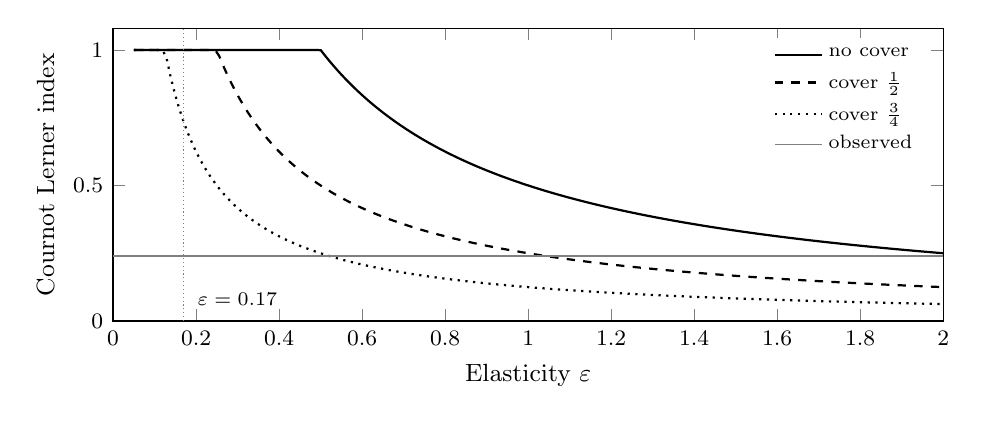
\begin{tikzpicture}
\begin{axis}[width=\linewidth, height=5.3cm, xmin=0, xmax=2, ymin=0, ymax=1.08,
  xlabel={\small Elasticity $\varepsilon$}, ylabel={\small Cournot Lerner index},
  tick label style={font=\footnotesize},
  legend style={font=\scriptsize, draw=none, fill=white, at={(0.98,0.97)}, anchor=north east},
  legend cell align=left]
\addplot[thick, domain=0.05:2, samples=200] {min(1, 0.5/x)};
\addlegendentry{no cover}
\addplot[thick, dashed, domain=0.05:2, samples=200] {min(1, 0.25/x)};
\addlegendentry{cover $\frac{1}{2}$}
\addplot[thick, dotted, domain=0.05:2, samples=200] {min(1, 0.125/x)};
\addlegendentry{cover $\frac{3}{4}$}
\addplot[gray, domain=0:2] {0.24};
\addlegendentry{observed}
\draw[gray, densely dotted] (axis cs:0.17,0) -- (axis cs:0.17,1.08);
\node[font=\scriptsize, anchor=west] at (axis cs:0.18,0.08) {$\varepsilon = 0.17$};
\end{axis}
\end{tikzpicture}
\caption{Cournot markups and contract cover}
\end{subfigure}
\caption{Why oligopoly theory predicts high electricity markups. Panel (a) is a schematic. The industry marginal cost
curve $MC(Q)$ ranks plants from cheapest to most expensive. Demand $D$ is nearly vertical, so withholding a quantity
$\Delta$ of low-cost capacity shifts the offered supply to $S^{w}$ and raises the price from $P^{c}$ to $P^{w}$. Panel
(b) plots the Cournot Lerner index $\min\{1, \frac{s_i}{\varepsilon}(1 - \frac{x_i}{q_i})\}$ of a firm with share
$s_i = \frac{1}{2}$ and contract cover $\frac{x_i}{q_i}$, from \eqref{eq:03-contracts}. Under constant-elasticity
demand, the value one marks the region with no interior equilibrium. The gray horizontal line is the observed average Lerner index of 0.24.}
\label{fig:03-merit-order}
\end{figure}

\subsection{Data and the measurement of marginal cost}\label{sec:03-wolfram-data}

\casehead{The data}
The sample covers 25,639 half-hour periods: nearly every half-hour of six months (January, February, March, April,
July and November) in each of 1992, 1993 and 1994, 18 months in all. About 40 periods are missing. The Pool data come
from the National Grid Company, which lacked some variables before 1992 \citep[pp.~810, 822 and n.~49]{Wolfram1999}.
Price is the SMP, which excludes the capacity payment, because the cost measure covers only fuel. Quantity is the
energy metered in each half-hour, including transmission losses. Appendix Table A1 of the paper reports a mean SMP of
\pounds 22.26 per megawatt-hour (MWh), with a standard deviation of 7.10. The pool selling price, which adds the
capacity payment and uplift, has a mean of \pounds 24.40 and a standard deviation of 10.17. Mean quantity is 16,211
MWh per half-hour, with a standard deviation of 2,839. Energy of 16,211 MWh delivered in half an hour is an average
rate of about 32 GW.

\casehead{Plant marginal cost}
The short-run marginal cost of a fossil-fuel plant is the cost of the fuel it burns per unit of electricity. Let plant
$k$ burn fuel with price $w_k$ in pounds per gigajoule (GJ) and convert fuel energy into electricity with
\emph{thermal efficiency} $e_k \in (0, 1)$. One MWh equals 3.6 GJ, so the plant needs $\frac{3.6}{e_k}$ GJ of fuel per
MWh, a quantity called its \emph{heat rate} $h_k$. Its marginal cost is
\begin{equation}\label{eq:03-plant-mc}
mc_k = w_k\, h_k = \frac{3.6\, w_k}{e_k} \quad \text{(pounds per MWh)}.
\end{equation}
For illustration, take coal at \pounds 1.50 per GJ plus \pounds 0.08 of transport and a hypothetical coal plant with an
efficiency of 36 percent. Then $mc_k = \frac{3.6 \times 1.58}{0.36} = 15.8$, inside the range of the flat coal segment of
\cref{fig:03-wolfram-scatter}.

Each input of \eqref{eq:03-plant-mc} is measured with unusual precision \citep[p.~810]{Wolfram1999}. Before
privatization, the \emph{CEGB Statistical Yearbook} published the thermal efficiency of every coal, oil and gas plant.
\citet{GreenNewbery1992} distilled 20 years of these figures into efficiencies under optimal operating conditions, and
Wolfram replaces them with later engineering estimates where plants had been upgraded. Such data later became
competitively sensitive. They are available only because the industry had recently been public. New combined-cycle gas
turbine (CCGT) plants are assumed to have an efficiency of 45 percent. Fuel prices for oil, gas peaking and CCGT plants
are market prices. Coal was bought from British Coal under contracts. The first contracts, which expired in March 1993,
were effectively take-or-pay and supplied more coal than the generators burned. To capture the replacement cost of coal,
Wolfram uses the prices of the next two contracts. Coal burned before the end of March 1994 is valued at 150 pence per
GJ, and coal burned afterwards at 137 pence. Transport costs average 8 pence per GJ, about 5 percent of fuel costs. Nuclear stations are
assigned \pounds 13 (Magnox, the first-generation gas-cooled reactors) and \pounds 11 (advanced gas-cooled reactors)
per MWh. These figures are too high, but
nuclear plants are never marginal. Pumped storage is costed at the average pool price during pumping, adjusted for
efficiency, and imports from Scotland and France at their bid prices.

\casehead{Capacity and the merit order}
A plant's available capacity varies with maintenance and age. Generators may also withhold capacity strategically to
raise capacity payments \citep{WolakPatrick1997}. Wolfram therefore assigns each plant a capacity equal to the mean
plus one half standard deviation of its declared daily capacity in the month. This is on average 85 percent of the
maximum capacity the plant declared for the year. Weighted by plant size the average is 100 percent. The high-availability case of \cref{tab:03-wolfram-robust}, the mean
plus a full standard deviation, raises the unweighted average to 92 percent \citep[pp.~810--811, 816]{Wolfram1999}.
Sorting plants by marginal cost
gives the industry marginal cost curve, called the \emph{merit order}. Index months by $\mu$, and let month $\mu$ have
plants ordered so that $mc_{(1)} \le mc_{(2)} \le \dots$, with capacities $K_{(1)}, K_{(2)}, \dots$. Then
\begin{equation}\label{eq:03-merit-order}
MC_\mu(Q) = mc_{(j)} \qquad \text{for } \sum_{l < j} K_{(l)} < Q \le \sum_{l \le j} K_{(l)}.
\end{equation}
This nondecreasing step function is the marginal cost of producing $Q$ at least cost. Each half-hour $t$ of month $\mu$
yields a markup $L_t = \frac{P_t - MC_\mu(Q_t)}{P_t}$.

\begin{remark}[What the merit-order cost measures]\label{rem:03-merit-order}
Without firm-level quantities, Wolfram cannot compute each firm's own marginal cost. The merit order supplies an
industry marginal cost directly. Under least-cost dispatch every running plant has $mc_k \le MC_\mu(Q_t)$ and the
marginal plant has exactly $MC_\mu(Q_t)$. If every firm operates a plant at the margin, then $MC_{it} = MC_\mu(Q_t)$ for
all $i$, and
any weights in \cref{prop:03-aggregation} give the same industry marginal cost. If firms withhold low-cost units, the
units that run are more expensive than least-cost dispatch requires. The measured markup then compares price with the
efficient marginal cost, so it also counts the productive inefficiency that withholding creates.
\end{remark}

\casehead{What the data show}
\Cref{fig:03-wolfram-scatter} reproduces the paper's Figure 2 for January and July 1993, a winter and a summer month at
the midpoint of the sample (n.~17). The marginal cost curve rises over the first few gigawatt-hours, where nuclear and
other cheap plants sit. It is then almost flat, between about \pounds 14 and \pounds 17 per MWh, over a wide range where
coal plants are marginal. Near capacity it turns almost vertical, around 26 to 28 GWh per half-hour in January and 21
to 23 GWh in July, when plants are out for summer maintenance. Every observed price lies above marginal cost. In January
prices run from about \pounds 17 to \pounds 35, and the gap widens with quantity. July prices are more dispersed, with a
band near \pounds 31 at low quantities, a cluster around \pounds 50 and one price above \pounds 100. Prices were more
volatile after March 1993, when the initial contracts expired (n.~17). The clouds sit on the flat part of the cost
curve, far from the steep segment where withholding by a duopoly would push them.

\begin{figure}[htbp]
\centering
\begin{subfigure}[b]{0.72\textwidth}
\centering
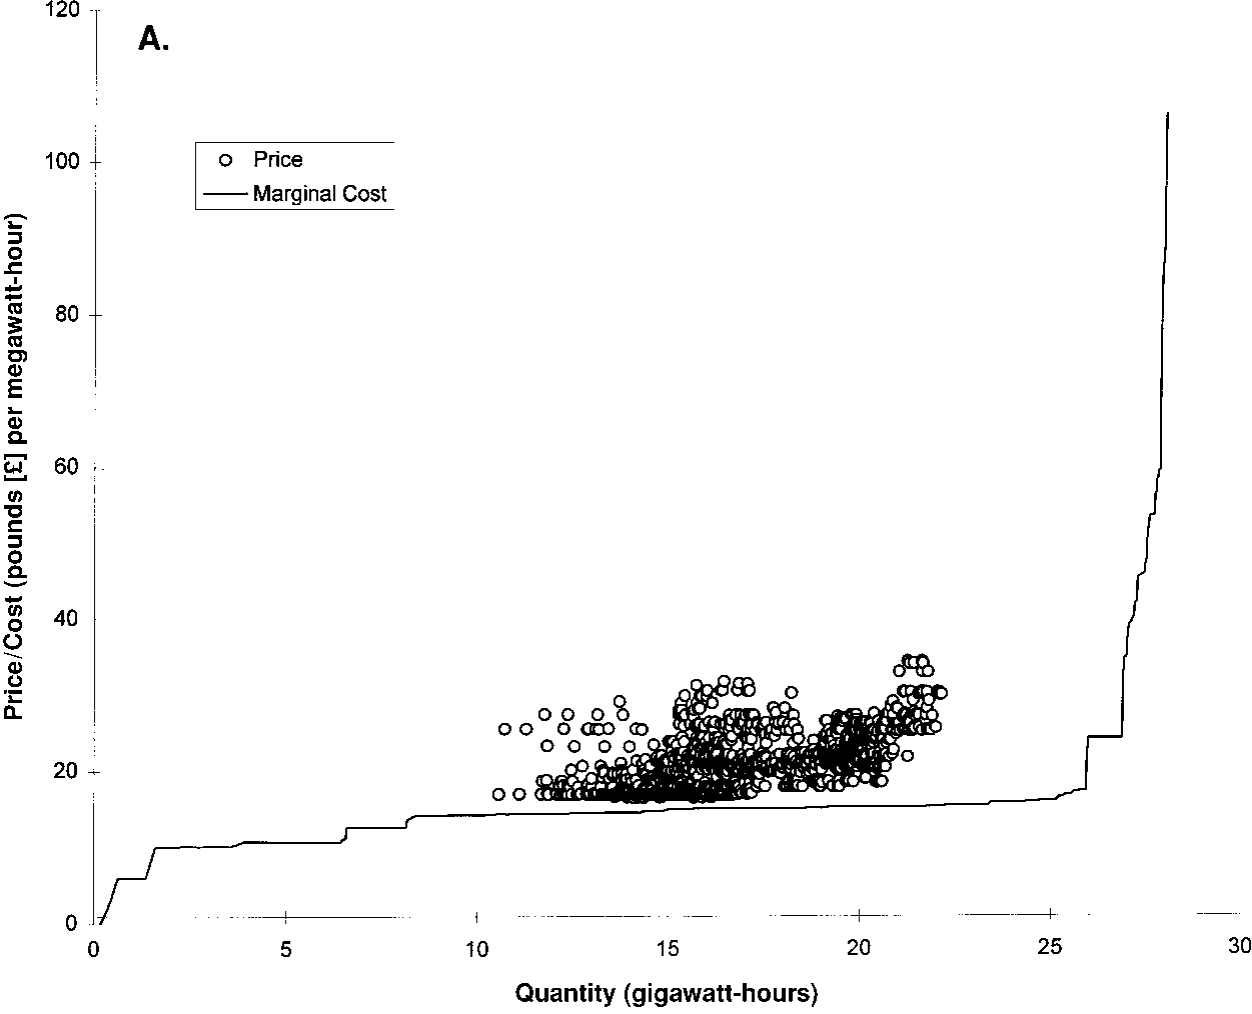
\includegraphics[width=\linewidth]{figures/ch03/wolfram1999_fig2a.png}
\caption{January 1993}
\end{subfigure}

\medskip
\begin{subfigure}[b]{0.72\textwidth}
\centering
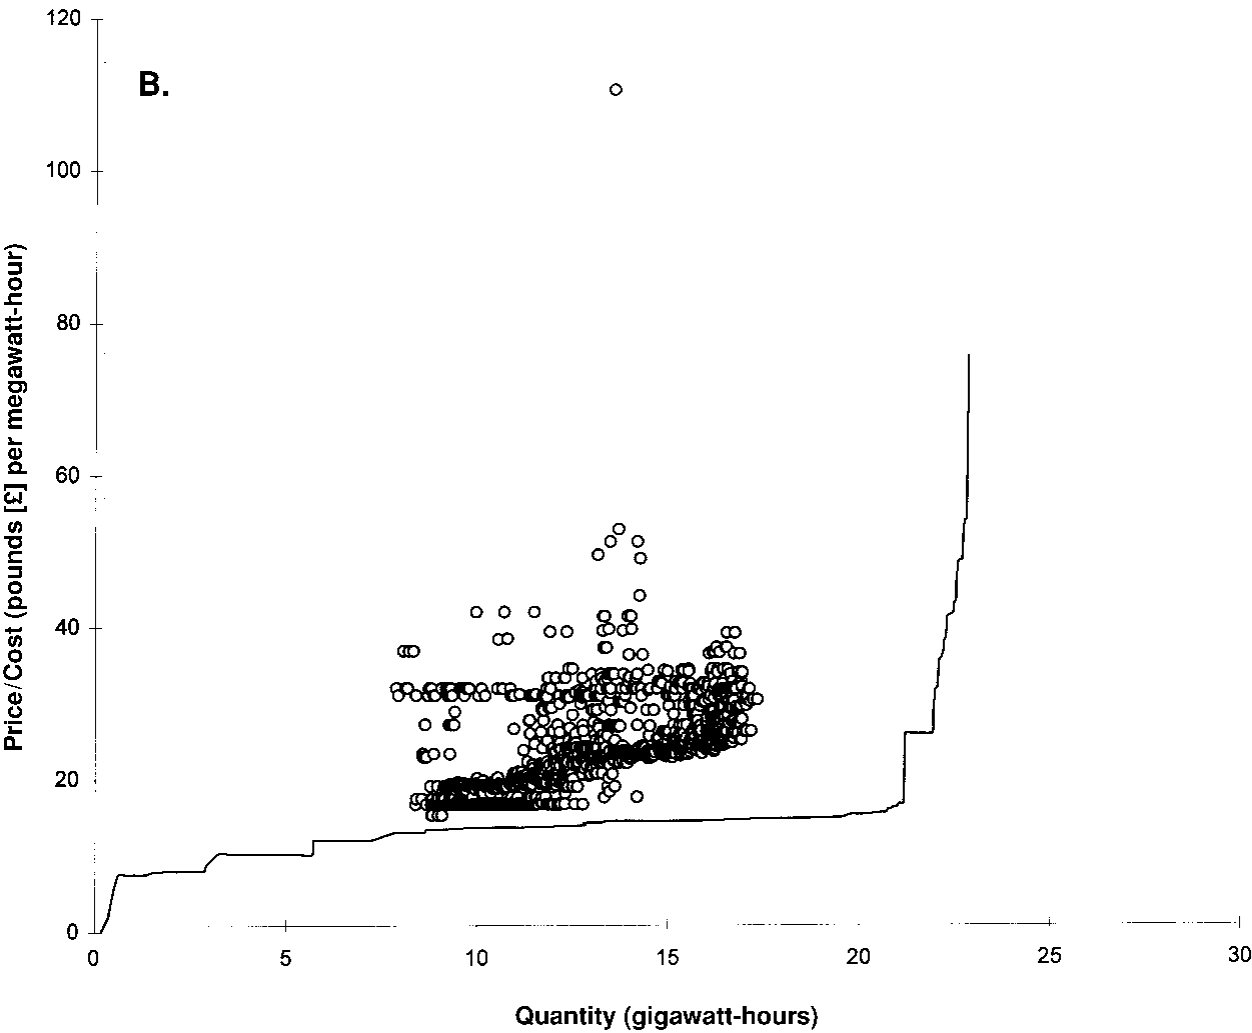
\includegraphics[width=\linewidth]{figures/ch03/wolfram1999_fig2b.png}
\caption{July 1993}
\end{subfigure}
\caption{Pool prices (circles, one per half-hour) and the merit-order marginal cost curve (line), in pounds per MWh
against quantity in gigawatt-hours per half-hour. Source: \citet{Wolfram1999}, Figure 2.}
\label{fig:03-wolfram-scatter}
\end{figure}

\subsection{The model and the direct measure of conduct}\label{sec:03-wolfram-model}

\casehead{Demand, cost and the firm supply relation}
Wolfram's framework is the supply relation of \cref{sec:03-framework} written for half-hours $t$
\citep[pp.~808--809]{Wolfram1999}. Demand is
\begin{equation*}
D_t = D(P_t, X_t, u^d_t),
\end{equation*}
with observed demand shifters $X_t$ such as weather and a demand shock $u^d_t$. Pool demand does respond to price. Some
large users buy directly from the Pool or on contracts tied to pool prices. They switch to backup generators, shut down
energy-intensive processes, or reschedule maintenance when prices are high. Demand also depends on prices in other
half-hours, which the notation suppresses (n.~10). Generator $i$ has marginal cost $MC_{it} = MC_i(q_{it}, Z_{it},
u^s_{it})$, with cost shifters $Z_{it}$ and a cost shock $u^s_{it}$, and profit
\begin{equation*}
\Pi_{it} = P(Q_t, X_t, u^d_t)\, q_{it} - C_i(q_{it}, Z_{it}, u^s_{it}).
\end{equation*}
Its first-order condition, written with a firm-level conduct parameter $\tilde\theta_{it}$, is
\begin{equation}\label{eq:03-wolfram-foc}
P_t = MC_i(q_{it}, Z_{it}, u^s_{it}) - \tilde\theta_{it}\, q_{it}\, P_Q(Q_t, X_t, u^d_t),
\end{equation}
where $P_Q$ is the slope of inverse demand. Cournot conduct is $\tilde\theta_{it} = 1$ and price taking is
$\tilde\theta_{it} = 0$. In the language of \cref{cor:03-benchmarks}, $\tilde\theta_{it} = 1 + r_i$.

\casehead{Aggregation}
Firm-level quantities are not available, so the analysis works with the industry. Applying
\cref{prop:03-aggregation} to \eqref{eq:03-wolfram-foc} with weights $\varphi_{it}$ gives
\begin{equation}\label{eq:03-wolfram-supply}
P_t = MC(Q_t, \mathbf{Z}_t, u^s_t) + \frac{P_t}{\varepsilon_t}\,\theta_t,
\qquad
\theta_t = \sum_{i=1}^{N} \varphi_{it}\,\frac{q_{it}}{Q_t}\,\tilde\theta_{it},
\end{equation}
which is Wolfram's eq.~(5). Rearranging gives her eq.~(6),
\begin{equation}\label{eq:03-wolfram-theta}
\theta_t = \varepsilon_t\,\frac{P_t - MC_t}{P_t}.
\end{equation}
Wolfram writes $\eta$ for the elasticity and $\kappa_{it}$ for the weights. With $\varphi_{it} = \frac{1}{N}$ and a common
$\tilde\theta_t$, industry conduct is $\theta_t = \frac{\tilde\theta_t}{N}$. It equals 1 for joint profit maximization,
$\frac{1}{N}$ for Cournot and 0 for perfect competition. For this reason $\frac{1}{\theta_t}$ is sometimes read as an
``equivalent number of firms.'' Wolfram treats $\theta_t$ as a summary measure, the elasticity-adjusted markup. She makes
no claim about the conjectures that firms hold (n.~12, citing \citealp{Corts1999}).

\begin{remark}[Markups as transfers]\label{rem:03-wolfram-welfare}
With very inelastic demand, even large markups cause little deadweight loss. Approximate demand by a straight line near
the equilibrium and take marginal cost as flat. Pricing at $P$ instead of $MC$ reduces quantity by about
$\varepsilon Q\frac{P - MC}{P}$, so the Harberger triangle is
\begin{equation*}
DWL \approx \frac{1}{2}(P - MC)\,\varepsilon Q\,\frac{P - MC}{P}
\qquad\Longrightarrow\qquad
\frac{DWL}{PQ} \approx \frac{1}{2}\,\varepsilon L^2 = \frac{1}{2}\,\theta L.
\end{equation*}
With $\varepsilon = 0.17$ and $L = 0.24$, the loss is about 0.5 percent of expenditure, while the transfer
$\frac{(P - MC)Q}{PQ} = L$ is 24 percent. This is why Wolfram also reports quantity-weighted average markups, which speak
to the surplus transferred to producers (p.~814).
\end{remark}

\casehead{The demand slope}
Marginal cost is measured, so only the elasticity is missing from \eqref{eq:03-wolfram-theta}. Wolfram does not
estimate it for this purpose. She assumes linear demand with slope $D_p = \frac{\partial D}{\partial P} = -125$, which
makes her numbers comparable with the simulations of \citet{GreenNewbery1992} \citep[p.~811]{Wolfram1999}. The units are
MWh per half-hour per pound per MWh. A fall of 125 MWh within a half-hour is an average rate of 250 megawatts, or
0.25 GW, which is the slope $b = 0.25$ that Green and Newbery report in gigawatts. Their low and high cases correspond to
$D_p = -50$ and $D_p = -250$. With linear demand,
\begin{equation}\label{eq:03-wolfram-theta-linear}
\varepsilon_t = -D_p\,\frac{P_t}{Q_t}
\qquad\Longrightarrow\qquad
\theta_t = \varepsilon_t\,\frac{P_t - MC_t}{P_t} = -D_p\,\frac{P_t - MC_t}{Q_t}.
\end{equation}
At the sample means, $\varepsilon = \frac{125 \times 22.26}{16{,}211} = 0.17$. This is in the range of short-run
elasticities found elsewhere \citep{Taylor1975}. The largest elasticity that \citet{PatrickWolak1997} find for customers
on pool-price contracts is about 0.3, for water companies, a group unusually sensitive to price. With an average Lerner
index of 0.241, \eqref{eq:03-wolfram-theta-linear} at the means gives $\theta = \frac{125 \times 0.241 \times
22.26}{16{,}211} = 0.041$.

Later work confirms that short-run electricity demand is very inelastic. One reason is that many households face
retail prices that do not vary with wholesale conditions \citep[p.~709]{KelloggReguant2021}. \citet{ReissWhite2005}
exploit the tiers of California tariffs in household survey data. They find an average elasticity of $-0.39$, which
reflects medium-run to long-run responses. \citet{Ito2014} compares households on either side of a utility border in
Orange County. He finds an elasticity of about $-0.08$ with respect to the average price. \citet{Shaffer2020} estimates
about $-0.04$ from bunching at a tariff kink in British Columbia \citep[pp.~710--711]{KelloggReguant2021}. These are
retail residential elasticities, and none measures the response of pool demand. Still, they bracket the value of 0.17
assumed here and the rotation estimates of about 0.1 in \cref{sec:03-wolfram-neio}.

\begin{example}[The Cournot benchmark under the assumed demand]\label{ex:03-wolfram-cournot}
Extend the linear demand through the sample means: $Q = 125(\bar\alpha - P)$ with choke price $\bar\alpha = 22.26 +
\frac{16{,}211}{125} = 151.95$. Let a symmetric duopoly have flat marginal cost $c = 16$, roughly the level of the coal
segment. Inverse demand is $P = \bar\alpha - \frac{Q}{125}$, and the symmetric Cournot price with $N$ firms is
$\frac{\bar\alpha + Nc}{N + 1}$. With $N = 2$,
\begin{equation*}
P^{C} = \frac{151.95 + 2 \times 16}{3} = 61.32,
\qquad
Q^{C} = 125\,(151.95 - 61.32) = 11{,}329.
\end{equation*}
The Lerner index is $\frac{61.32 - 16}{61.32} = 0.74$. The elasticity at this point is
$\frac{125 \times 61.32}{11{,}329} = 0.68$, and $\theta = 0.68 \times 0.74 = 0.5 = \frac{1}{N}$, as it must be. The
benchmark price is almost three times the mean SMP. The calculation extrapolates the linear demand far outside the
sample and is only an illustration of the scale of the predicted markups.
\end{example}

\casehead{Benchmarks for conduct}
Price taking gives $\theta = 0$ and joint profit maximization gives $\theta = 1$. Cournot gives
$\theta = \sum_i \varphi_{it} s_{it}$ (\cref{cor:03-benchmarks}). This is $\frac{1}{2}$ for a symmetric duopoly. For the
two asymmetric generators, Wolfram uses 0.52 (p.~818). That value matches a Herfindahl index computed with shares in the
ratio of the initial capacities, $\bigl(\frac{52}{85}\bigr)^2 + \bigl(\frac{33}{85}\bigr)^2 = 0.52$. The fourth
benchmark comes from a model built for electricity markets.

\casehead{Supply function equilibrium}
In the Pool, firms bid supply schedules that state a price for each quantity. \citet{KlempererMeyer1989} model such
competition. Each firm commits to a supply function before a demand shock is realized, and the market clears where total supply meets
demand. \citet{GreenNewbery1992} were the first to apply the concept to the Pool. They calibrate cost functions for the
two effective duopolists and a demand curve, and they solve for the supply function equilibria, including asymmetric
ones. The equilibria range from marginal-cost pricing to one that reproduces the Cournot quantities and prices. The
highest-price equilibrium implies large markups. Observed prices showed no such markups, and Green and Newbery
suggest that the generators' forward sales of much of their capacity may explain the gap. A long-run version of the model finds that
entry incentives depend strongly on the demand elasticity and on the incumbents' pricing strategies
\citep[pp.~145--146]{HortacsuPerrigne2021}. \citet{Wolfram1998} later treated the bids as a uniform-price multi-unit
auction. A higher bid raises the price paid on all accepted units if it sets the price, but it lowers the chance that
the unit is accepted \citep[p.~695]{KelloggReguant2021}. Her evidence is consistent with strategic withholding of
supply \citep[p.~146]{HortacsuPerrigne2021}.
The next result derives the equilibrium condition and shows where supply function markups fall. \Cref{rem:02-sfe}
states its Lerner form without proof.

\begin{proposition}[Supply function equilibrium markups]\label{prop:03-sfe-markup}
Two firms have cost functions $C_i$ with $C_i' \ge 0$. Demand is $D(P) + u$, with $D' < 0$ and a shock $u$ whose support
is an interval. Before $u$ is known, firm $i$ chooses a differentiable, nondecreasing, nonnegative supply function
$S_i(P)$, and the price clears $S_1(P) + S_2(P) = D(P) + u$. Suppose each $S_i$ maximizes firm $i$'s profit for every
realization of $u$, given $S_j$. Then at every clearing price at which firm $i$ sells a positive quantity,
\begin{equation}\label{eq:03-sfe-ode}
S_i(P) = \bigl(P - C_i'(S_i(P))\bigr)\bigl(S_j'(P) - D'(P)\bigr), \qquad i \ne j.
\end{equation}
At a clearing price with $S_i(P) = 0$, optimality requires only $P \le C_i'(0)$. If both firms sell positive
quantities at $P$, the Lerner index of firm $i$ is
\begin{equation}\label{eq:03-sfe-lerner}
L_i = \frac{s_i}{\varepsilon + s_j\,\eta_j}, \qquad \eta_j = \frac{P\,S_j'(P)}{S_j(P)} \ge 0,
\end{equation}
where $s_i = \frac{S_i}{Q}$ and $\varepsilon = -\frac{P D'(P)}{Q}$. Hence $0 < L_i \le \frac{s_i}{\varepsilon}$, and
firm $i$'s conduct parameter is $\tilde\theta_i = \frac{\varepsilon}{\varepsilon + s_j\eta_j} \in (0, 1]$.
\end{proposition}

\begin{proof}
Fix $S_j$ and a realization $u$. Whatever $S_i$ is, firm $i$ ends up at some price $P$ and sells its residual demand
$R_i(P, u) = D(P) + u - S_j(P)$. Since supply cannot be negative, only prices with $R_i(P, u) \ge 0$ can clear the
market. Choosing a supply function is therefore equivalent to choosing, for each $u$, such a price on the residual
demand curve. Profit at price $P$ is $\pi_i(P, u) = P R_i(P, u) - C_i(R_i(P, u))$, with derivative
\begin{equation*}
\frac{\partial \pi_i}{\partial P} = R_i(P, u) + \bigl(P - C_i'(R_i(P, u))\bigr)\bigl(D'(P) - S_j'(P)\bigr).
\end{equation*}
Residual demand strictly decreases in $P$, because $D' - S_j' < 0$. If the optimal price leaves firm $i$ a positive
quantity, nearby prices are also feasible, so the derivative is zero there. If it leaves the firm nothing, only lower
prices are feasible, and lowering the price must not raise profit. The derivative is then nonnegative. With
$R_i = 0$ it equals $\bigl(P - C_i'(0)\bigr)(D' - S_j')$, so this holds exactly when $P \le C_i'(0)$.
The shock shifts residual demand horizontally without changing its slope, so different realizations select different
optimal prices. The supply function $S_i$ implements all these optima only if $S_i(P) = R_i(P, u)$ at each optimal pair.
Setting the derivative to zero then gives \eqref{eq:03-sfe-ode} wherever $S_i(P) > 0$. Its left side is positive, so
$P > C_i'$ and $L_i > 0$. When $S_j(P) > 0$ as well, divide \eqref{eq:03-sfe-ode} by $P$ and then numerator and
denominator by $Q$:
\begin{equation*}
\frac{P - C_i'}{P} = \frac{S_i}{P(S_j' - D')} = \frac{\frac{S_i}{Q}}{\frac{S_j}{Q}\cdot\frac{P S_j'}{S_j} -
\frac{P D'}{Q}} = \frac{s_i}{s_j\eta_j + \varepsilon}.
\end{equation*}
Since $\eta_j \ge 0$, $L_i \le \frac{s_i}{\varepsilon}$. Comparing with the firm supply relation
$L_i = \tilde\theta_i\frac{s_i}{\varepsilon}$ of \cref{prop:03-aggregation} gives $\tilde\theta_i$.
\end{proof}

The equality \eqref{eq:03-sfe-ode} is required only of active firms. With asymmetric costs, a high-cost firm can optimally supply nothing
at some or all clearing prices. Its condition then holds only as the inequality $P \le C_i'(0)$.
The proposition places supply function equilibria between competition and Cournot. If the rival's supply does not
respond to price ($\eta_j = 0$), firm $i$ faces the Cournot residual demand. As the rival's supply becomes very elastic
($\eta_j \to \infty$), the markup goes to zero. The formula also shows why the concept suits electricity. As demand
becomes perfectly inelastic, the Cournot markup explodes, while the supply function markup stays finite at
$\frac{s_i}{s_j\eta_j}$, disciplined by the rival's supply response. In a symmetric equilibrium with positive supply,
\eqref{eq:03-sfe-ode} becomes
the differential equation $S'(P) = \frac{S(P)}{P - C'(S(P))} + D'(P)$, which has a continuum of solutions. Klemperer and
Meyer show that the equilibria form a range when the shock has bounded support. Wolfram computes the \emph{highest}
supply function equilibrium, the solution that passes through the symmetric Cournot point on the right-most demand
curve (pp.~813--814). Following Green and Newbery, she assumes a symmetric duopoly. The right-most demand curve has slope
$-125$ and passes through the monopoly price at a quantity of 30 in the gigawatt units of the paper. The largest
quantity in the sample is 24, so this choice is conservative (n.~22). The benchmark $\theta$ is the margin in the supply function equilibrium
times the elasticity under $D_p = -125$. Both are evaluated at the equilibrium point, where the price is higher and the
elasticity larger than in the data. Because marginal cost rises
so steeply, the lowest supply function equilibrium gives very similar markups (n.~23).

\subsection{Markups and conduct}\label{sec:03-wolfram-results}

\Cref{tab:03-wolfram} reproduces Table~1 of \citet{Wolfram1999}. Each entry averages over half-hours, and the
standard deviations in parentheses describe the dispersion across half-hours. The first column is the Lerner index
computed from the merit order. The second multiplies each half-hour's Lerner index by its elasticity under $D_p = -125$,
as in \eqref{eq:03-wolfram-theta-linear}. The third gives $\theta$ in the highest supply function equilibrium.

\begin{table}[htbp]
\centering
\begin{threeparttable}
\caption{Price-cost markups calculated with measured marginal cost}
\label{tab:03-wolfram}
\small
\setlength{\tabcolsep}{4.5pt}
\begin{tabular}{@{}lcccc@{}}
\toprule
& (i) & (ii) & (iii) & (iv) \\
Period & $\frac{P - MC}{P}$ & $\theta = \varepsilon\frac{P - MC}{P}$ & $\theta$, highest SFE & Observations \\
\midrule
Jan.~1992 to Mar.~1993 & 0.241 (0.129) & 0.043 (0.030) & 0.28 (0.06) & 12,704 \\
Apr.~1993 to Mar.~1994 & 0.259 (0.228) & 0.057 (0.055) & 0.29 (0.06) & 8,637 \\
After Mar.~1994 & 0.208 (0.416) & 0.067 (0.086) & 0.33 (0.07) & 4,298 \\
\addlinespace
Four weeks before a regulatory decision & 0.329 (0.150) & 0.071 (0.051) & & 3,216 \\
Four weeks after a regulatory decision & 0.156 (0.213) & 0.028 (0.040) & & 2,671 \\
\addlinespace
\multicolumn{5}{@{}l}{\emph{By quantity level}} \\
Jan.~1992 to Mar.~1993, above median & 0.279 (0.124) & 0.046 (0.027) & 0.31 (0.05) & 6,764 \\
\phantom{Jan.~1992 to Mar.~1993,} below median & 0.198 (0.121) & 0.039 (0.033) & 0.23 (0.02) & 5,940 \\
Apr.~1993 to Mar.~1994, above median & 0.299 (0.184) & 0.056 (0.044) & 0.33 (0.05) & 4,530 \\
\phantom{Apr.~1993 to Mar.~1994,} below median & 0.214 (0.261) & 0.058 (0.065) & 0.24 (0.02) & 4,107 \\
After Mar.~1994, above median & 0.554 (0.122) & 0.138 (0.057) & 0.37 (0.09) & 1,526 \\
\phantom{After Mar.~1994,} below median & 0.018 (0.398) & 0.027 (0.073) & 0.26 (0.02) & 2,772 \\
\bottomrule
\end{tabular}
\begin{tablenotes}\footnotesize
\item Notes: Reproduced from \citet{Wolfram1999}, Table~1. The unit of observation is a half-hour. Standard deviations
across half-hours in parentheses. Columns (ii) and (iii) assume linear demand with slope $D_p = -125$, so that
$\varepsilon = -D_p\frac{P}{Q}$. SFE: supply function equilibrium. The three periods sum to 25,639 half-hours, and each
pair of quantity rows sums to its period total. Column (ii) is a mean of ratios, so it differs from column (i) times
0.17.
\end{tablenotes}
\end{threeparttable}
\end{table}

\casehead{Levels}
Prices exceed measured marginal cost by more than 20 percent on average, so the market is far from competitive. The
averages are precise. Two-sided $t$-tests at the 1 percent level reject an average markup below 0.19 in the last period
and above 0.245 in the first. Serial correlation makes these tests somewhat optimistic (p.~811 and n.~21).
Conduct, however, is small. The values of $\theta$ between 0.043 and 0.067 are far from collusion ($\theta = 1$) and far
below Cournot (0.5 or 0.52). They are also far below the highest supply function equilibrium, between 0.28 and 0.33. A
value of 0.05 corresponds to symmetric Cournot competition among 20 firms. The values are significantly above zero, so
the Bertrand model of homogeneous price competition is rejected as well. Wolfram notes features that should have made
collusion easy (p.~813). The firms bid daily, an infinitely repeated game, and as former parts of one organization they
knew each other's plants well.

How wrong would the assumed elasticity have to be to reverse these conclusions? Column (ii) is column (i) times the
elasticity. Joint profit maximization would require an elasticity of about $\frac{1}{0.25} = 4$, and asymmetric Cournot
conduct one of about $\frac{0.52}{0.25} = 2.1$. Matching the highest supply function equilibrium would require an
elasticity above about 3, because that benchmark itself rises as demand becomes more elastic (p.~818). Even long-run electricity elasticities rarely exceed 1.5 \citep{Taylor1975}. The
qualitative conclusion
is therefore robust to the demand assumption, even though the level of $\theta$ is not.

\casehead{Patterns}
Markups rise with quantity, mildly before April 1994 and dramatically afterwards: 0.554 above the median quantity
against 0.018 below. The price cap explains the later pattern. It applied to the time-weighted average price, so the
generators could stay under it by cutting prices when demand was low and raising them when demand was high (p.~814).
Quantity-weighted averages, which track the surplus transferred, are close to the time-weighted ones before April 1994,
at 0.248 and 0.264. After March 1994 the quantity-weighted average is 0.262, against a time-weighted 0.208. Markups are
also much higher in the four weeks before a regulatory decision (0.329) than in the four weeks after (0.156). The
dispersion across half-hours is large, with standard deviations comparable to the means. Variation by quantity explains
less than 5 percent of it (n.~26). Within a month the merit-order curve is fixed, but marginal cost still moves along
it as quantity changes. The plants at the margin over much of the observed range have similar costs, so the curve is
nearly flat there (\cref{fig:03-wolfram-scatter}). Wolfram therefore attributes the volatility of markups primarily to
prices (n.~26).

\casehead{Robustness}
\Cref{tab:03-wolfram-robust} reproduces the paper's Table~2. High fuel costs value coal at the take-or-pay contract price
of 180 pence per GJ before April 1993. They also raise oil and gas prices by 20 percent and add \pounds 1 per MWh to
nuclear costs.
Low fuel costs set coal at world prices (120 and then 110 pence per GJ) and lower the other fuels symmetrically. Low and
high availability assign each plant the monthly mean, or the mean plus a full standard deviation, of its declared
capacity. The last column measures the margin against the pool selling price, which adds capacity payments and uplift
to the SMP.

\begin{table}[htbp]
\centering
\begin{threeparttable}
\caption{Lerner indices under alternative assumptions}
\label{tab:03-wolfram-robust}
\small
\setlength{\tabcolsep}{4pt}
\begin{tabular}{@{}lccccccc@{}}
\toprule
& & \multicolumn{2}{c}{Fuel prices} & \multicolumn{3}{c}{Plant capacity} & \\
\cmidrule(lr){3-4}\cmidrule(lr){5-7}
& (i) & (ii) & (iii) & (iv) & (v) & (vi) & (vii) \\
Period & Benchmark & High & Low & \makecell{Low\\avail.} & \makecell{High\\avail.} & Declared &
  \makecell{Pool selling\\price} \\
\midrule
Jan.\ 1992 to Mar.\ 1993 & \makecell{0.241\\(0.129)} & \makecell{0.097\\(0.154)} & \makecell{0.384\\(0.105)} &
  \makecell{0.231\\(0.130)} & \makecell{0.250\\(0.127)} & \makecell{0.231\\(0.130)} & \makecell{0.278\\(0.147)} \\
\addlinespace
Apr.\ 1993 to Mar.\ 1994 & \makecell{0.259\\(0.228)} & \makecell{0.119\\(0.269)} & \makecell{0.399\\(0.184)} &
  \makecell{0.246\\(0.231)} & \makecell{0.268\\(0.226)} & \makecell{0.245\\(0.233)} & \makecell{0.314\\(0.233)} \\
\addlinespace
After Mar.\ 1994 & \makecell{0.208\\(0.416)} & \makecell{0.179\\(0.432)} & \makecell{0.338\\(0.352)} &
  \makecell{0.196\\(0.421)} & \makecell{0.215\\(0.415)} & \makecell{0.195\\(0.422)} & \makecell{0.270\\(0.417)} \\
\bottomrule
\end{tabular}
\begin{tablenotes}\footnotesize
\item Notes: Reproduced from \citet{Wolfram1999}, Table~2. Entries are average Lerner indices $\frac{P - MC}{P}$ with
standard deviations across half-hours in parentheses. Column (i) is column (i) of \cref{tab:03-wolfram}. Column (vi)
uses each plant's actual declared daily capacity. Observations: 12,704, 8,637 and 4,298.
\end{tablenotes}
\end{threeparttable}
\end{table}

Markups are sensitive to fuel costs. Before April 1994 the two fuel cases move them by 54 to 60 percent in each
direction. After March 1994 the high-cost case lowers them by only 14 percent, while the low-cost case raises them by
about 63 percent. Markups are much less sensitive to availability. About 90 percent of the fuel-cost sensitivity comes from the coal assumptions. Coal plants set
the price most of the time, and in the 12 months to March 1997 they set the SMP in 82 percent of half-hours
(n.~33). Changing coal costs shifts the long flat segment of the merit order, which moves almost every markup.
Changing availability only lengthens or shortens that segment. Margins over the pool selling price are 15 to 30 percent
higher, because the extra charges are 5 to 10 percent of the pool price.

Three further checks support the cost measure \citep[p.~817]{Wolfram1999}. First, it implies producer surplus of about
25 percent of the generators' SMP revenue. SMP is about 90 percent of the pool price, and pool revenue is about 70
percent of National Power's total revenue. Fuel costs are therefore about $0.75 \times 0.9 \times 0.7 = 47$ percent of
revenue, close to the 40 and 45 percent reported in the two companies' 1994 annual reports. Second, a regression version
of \eqref{eq:03-wolfram-supply} imposes constant conduct and a constant elasticity. Solving $P_t = MC_t +
\frac{P_t}{\varepsilon}\theta$ for $P_t$ gives Wolfram's eq.~(7),
\begin{equation}\label{eq:03-wolfram-omega}
P_t = \omega\, MC_t + e_t, \qquad \omega = \frac{\varepsilon}{\varepsilon - \theta}.
\end{equation}
The coefficient $\omega$ is the constant-elasticity pass-through rate of \cref{cor:03-passthrough-cases}, with total
marginal cost in place of a tax. On all the data $\hat\omega = 1.92$ (robust standard error 0.75), which implies
$\theta = \varepsilon(1 - \frac{1}{\hat\omega}) = 0.17 \times (1 - \frac{1}{1.92}) = 0.081$. Instrumenting marginal cost
with the demand shifters, to address measurement error, raises the estimate slightly and insignificantly. Third, the
functional form of demand matters little. With a constant elasticity of 0.17, $\theta$ is 0.041, 0.044 and 0.035 in the
three periods. With a concave demand curve whose elasticity is 0.17 at the means, it is 0.043, 0.060 and 0.077
(n.~37).

\subsection{Why are markups so low?}\label{sec:03-wolfram-explanations}

Prices respond to the generators' incentives, yet they stay far below static oligopoly predictions. Wolfram weighs
three explanations (pp.~814--815): contracts, the threat of regulation, and the threat of entry.

\casehead{Contracts}
A generator that has sold part of its output forward gains less from a high spot price. The next result makes this
precise. It is the spot-market stage of the model of \citet{AllazVila1993}, and it restates \cref{ex:02-forward}.

\begin{proposition}[Forward contracts and spot markups]\label{prop:03-contracts}
Firm $i$ holds two-way contracts for $x_i$ units at strike price $F_i$ and then chooses its output $q_i$ as a Cournot
competitor. Its profit is
\begin{equation*}
\Pi_i = P(Q)\,(q_i - x_i) + F_i\, x_i - C_i(q_i),
\end{equation*}
and at an interior optimum
\begin{equation}\label{eq:03-contracts}
L_i = \frac{P - MC_i}{P} = \frac{s_i}{\varepsilon}\Bigl(1 - \frac{x_i}{q_i}\Bigr).
\end{equation}
\end{proposition}

\begin{proof}
The firm sells $q_i$ at the spot price and pays $(P - F_i)x_i$ on its contracts, so
$\Pi_i = P q_i - (P - F_i)x_i - C_i(q_i) = P(q_i - x_i) + F_i x_i - C_i(q_i)$. The first-order condition is
\begin{equation*}
P + P'(Q)\,(q_i - x_i) - MC_i = 0
\quad\Longrightarrow\quad
P - MC_i = -P'(Q)\, q_i\Bigl(1 - \frac{x_i}{q_i}\Bigr).
\end{equation*}
Dividing by $P$ and using $-\frac{P' Q}{P} = \frac{1}{\varepsilon}$ and $\frac{q_i}{Q} = s_i$ gives
\eqref{eq:03-contracts}.
\end{proof}

The firm cares about the price only on its uncontracted output $q_i - x_i$. Full cover makes it a price taker, and
cover above output makes it want a price below marginal cost. In conduct terms, $\tilde\theta_i = 1 - \frac{x_i}{q_i}$.
A one-way contract works differently. The generator refunds the excess of the pool price over the strike price, so cover
dampens its incentive only when the price is above the strike. Panel (b) of \cref{fig:03-merit-order} plots
\eqref{eq:03-contracts} for a firm with half the market.

The British data allow a test. Wolfram estimates that the initial contracts covered about 75 percent of the generators'
output and their replacements about half (p.~814). At the observed point, with $s_i = 0.5$ and $\varepsilon = 0.17$,
\eqref{eq:03-contracts} requires $L_i = \frac{0.5}{0.17}\times 0.25 = 0.74$ under the initial contracts and
$L_i = \frac{0.5}{0.17}\times 0.5 = 1.47$ under the replacements. The observed prices and quantities therefore cannot
be a Cournot equilibrium with either level of cover. What happens away from the observed point depends on the shape of
demand. Under a constant elasticity of 0.17, half cover would leave no interior equilibrium. Under the linear demand
of \cref{ex:03-wolfram-cournot}, the elasticity rises with the price, and an interior equilibrium exists for both
levels of cover. Write $\zeta = \frac{x_i}{q_i}$ for the cover ratio and take $c = 16$. The first-order condition
of \cref{prop:03-contracts} reads $P - c = \frac{(1 - \zeta)\, q_i}{125}$. In a symmetric duopoly
$q_i = \frac{125(\bar\alpha - P)}{2}$, so
\begin{equation*}
P - c = \frac{(1 - \zeta)(\bar\alpha - P)}{2}
\quad\Longrightarrow\quad
P - c = \frac{(1 - \zeta)(\bar\alpha - c)}{3 - \zeta},
\end{equation*}
which gives a price of 31.11 with 75 percent cover and 43.19 with half cover. The Lerner indices are 0.49 and 0.63. Either
way the model predicts a sharp rise after March 1993. \Cref{tab:03-wolfram} shows a rise from 0.241 to 0.259. A
fall of more than 20 percentage points in contract cover raised markups by less than 2 percentage points. Contracts
may restrain prices slightly, but they cannot explain why oligopoly models predict so poorly.

The contracts in Britain were imposed at privatization. \citet{AllazVila1993} show that duopolists choose to sell
forward even when nobody forces them to. The following example shows the mechanism in the simplest case.
\Cref{sec:02-forward} sketches the same calculation, and we give it in full here.

\begin{example}[Strategic forward sales]\label{ex:03-allaz-vila}
Two firms with constant marginal cost $c$ face inverse demand $P = a - bQ$. In stage 1 each firm sells $x_i$ forward.
Arbitrage sets the forward price equal to the spot price, which is known in this deterministic model. In stage 2 the
firms choose outputs. Stage-2 first-order conditions from \cref{prop:03-contracts} are
\begin{equation*}
a - b(q_i + q_j) - b(q_i - x_i) - c = 0, \qquad i = 1, 2,
\end{equation*}
so that
\begin{equation*}
q_i = \frac{a - c + 2b x_i - b x_j}{3b},
\qquad
P - c = \frac{a - c - b(x_i + x_j)}{3}.
\end{equation*}
A forward sale raises the firm's own output by $\frac{2}{3}$ and lowers the price by $\frac{b}{3}$ per unit. Since the
forward price equals the spot price, firm $i$'s total profit is $(P - c)q_i$. Its stage-1 condition is
\begin{equation*}
-\frac{b}{3}\, q_i + \frac{2}{3}(P - c) = 0
\quad\Longrightarrow\quad
P - c = \frac{b\, q_i}{2}.
\end{equation*}
In a symmetric equilibrium, substituting $q = \frac{a - c + bx}{3b}$ and $P - c = \frac{a - c - 2bx}{3}$ gives
\begin{equation*}
\frac{a - c - 2bx}{3} = \frac{a - c + bx}{6}
\quad\Longrightarrow\quad
x = \frac{a - c}{5b}, \qquad q = \frac{2(a - c)}{5b}, \qquad P - c = \frac{a - c}{5}.
\end{equation*}
Each firm covers half of its output. The margin falls from the Cournot level $\frac{a - c}{3}$ to $\frac{a - c}{5}$,
and both firms earn less. Each sells forward to commit itself to aggressive spot behavior, a prisoner's dilemma.
\end{example}

\citet{Green1999} builds contracts into the supply function framework and shows that pool prices fall as contract
cover rises \citep[p.~810]{Wolfram1999}. Contracts are therefore a coherent mechanism. The British evidence suggests that
they were not the main force restraining prices.

\casehead{The threat of regulation}
Prices react to the regulator's calendar. In the four weeks before OFFER's statements on pool prices the Lerner index
averages 0.329, and in the four weeks after it averages 0.156. Two-sided $t$-tests reject that markups around these
decisions equal markups at other times, and the differences persist after controlling for demand factors (n.~27). The
generators knew when a statement was being prepared, and the regulator analyzed prices from earlier months. Wolfram
suggests that the generators raised prices while the regulator could not yet see them and restrained prices afterwards,
when attention was on the Pool (pp.~814--815). In the model of \citet{GlazerMcMillan1992}, the threat of regulation
leads a monopolist to price below the monopoly level. The firm raises its price as the probability of future
regulation rises. The response to the 1994 price cap, documented above, is direct evidence that regulation shaped
pricing, and of the distortions a cap on average prices creates.

\casehead{The threat of entry}
Two pieces of evidence point to entry deterrence (p.~815). First, pool prices sat just below the long-run average cost
of a new entrant. Following Green and Newbery, a new CCGT plant had capital and non-fuel operating costs of roughly
\pounds 85 per kilowatt of capacity. Treating this as an annual cost, a plant that runs 90 to 95 percent of the year has
non-fuel costs of $\frac{85{,}000}{8{,}760 \times 0.95} = 10.2$ to $\frac{85{,}000}{8{,}760 \times 0.90} = 10.8$ pounds
per MWh. Adding
fuel costs of roughly \pounds 16 gives an average cost of \pounds 26 to \pounds 27 per MWh. Pool prices averaged
\pounds 23.6 per MWh in fiscal years 1993 and 1994. Second, pool prices moved with the price of natural gas, the fuel
of potential entrants, even in high-demand periods when no existing CCGT plant was marginal. In a regression of the
pool price on the demand variables and the gas price interacted with a dummy for demand above 15 GW, the gas coefficient
is 0.024 (standard error 0.008). A 10 percent rise in the gas price thus raises the pool price by less than 1 percent.
Pricing just below the entrant's cost would imply a nearly one-to-one relation between gas and pool prices. Wolfram
suggests that the generators may follow a more complex strategy, or that the gas price an entrant faces is measured
with error (n.~29).

\emph{Limit pricing} of this kind keeps prices low to make entry unprofitable. Game-theoretic models of limit pricing
rely on entrants being uncertain about incumbents' costs, which is implausible here, although entrants could be unsure
about regulatory constraints (n.~30). Some entry did occur. All independent plants added after privatization were at
least partly owned by RECs, which could pass their costs to franchise customers whatever the pool price. Entry decisions
may therefore have depended on more than pool prices.

\subsection{Estimates that ignore cost data}\label{sec:03-wolfram-neio}

Section~IV of the paper asks what a researcher without cost data would conclude. Wolfram applies two methods. The first
is new and exploits the distortion created by the price cap. The second is the demand-rotation approach of
\cref{sec:03-identification}.

\casehead{A bound from the price cap}
The cap on the time-weighted average price rotated the industry supply curve counterclockwise. Prices fell at low
demand and rose at high demand. \Cref{fig:03-pricecap-rotation} redraws the paper's stylized Figure~3. Wolfram sorts
half-hours into 25 groups by quantity, in bands of 0.5 GWh. For each group $g$ she compares the average price after the
cap, $P_{H,g}$, with the average price before, $P_{L,g}$. The \emph{rotation axis} is the lowest quantity at which prices
after the cap exceed prices before. Eleven groups lie to its left and fourteen to its right.

\begin{figure}[htbp]
\centering
\begin{tikzpicture}[scale=0.9,>=Stealth]
\draw[->] (0,0) -- (6.6,0) node[below] {\small $Q$};
\draw[->] (0,0) -- (0,4.7) node[left] {\small $P$};
\draw[thick] (0.5,0.8) -- (5.5,4.2);
\draw[thick,dashed] (0.5,1.5) -- (5.5,3.0);
\draw[thick,gray] plot[domain=0.5:5.6,samples=60] (\x,{0.45+0.012*\x*\x+0.6*exp(2.2*(\x-5.6))});
\draw[densely dotted] (2.342,0) -- (2.342,4.4);
\node[font=\footnotesize,align=center] at (2.342,4.6) {rotation axis};
\draw[decorate,decoration={brace,amplitude=4pt}] (5.6,4.2) -- (5.6,3.0);
\node[font=\footnotesize,anchor=west] at (5.75,3.6) {$P_{H} - P_{L}$};
\node[font=\footnotesize,anchor=south east] at (4.9,3.95) {after cap};
\node[font=\footnotesize,anchor=north west] at (3.9,2.45) {before cap};
\node[font=\footnotesize,gray,anchor=north] at (4.3,0.6) {marginal cost};
\end{tikzpicture}
\caption{The price cap rotates the supply relation. The solid and dashed lines are average prices by quantity after and
before the cap of April 1994. To the right of the rotation axis the normalized gap $\frac{P_H - P_L}{P_H}$ bounds the
Lerner index from below. The gap $P_H - P_L$ itself bounds the markup $P_H - MC$ from below.
Schematic redrawn after \citet{Wolfram1999}, Figure~3.}
\label{fig:03-pricecap-rotation}
\end{figure}

The logic is a revealed-preference bound. Suppose prices before the cap were at least as high as marginal cost after
the cap, $P_{L,g} \ge MC_g$. Then for each group to the right of the axis
\begin{equation}\label{eq:03-rotation-bound}
\frac{P_{H,g} - P_{L,g}}{P_{H,g}} \le \frac{P_{H,g} - MC_g}{P_{H,g}} = L_g.
\end{equation}
The condition holds if the generators priced at or above cost before the cap and costs did not rise. The coal price
fell from 150 to 137 pence per GJ in April 1994, which only helps. Averaging the left side over the fourteen groups,
weighted by their numbers of half-hours, gives 0.277 (standard deviation 0.145). If prices had equaled marginal cost
before the cap, this would approximate the Lerner index above the median quantity after March 1994. That index is 0.554
in \cref{tab:03-wolfram}, so the bound captures about half of the measured markup (p.~819). Groups to the left of the
axis are excluded, because the generators may have priced below cost at low demand to stay under the cap (n.~39). The
method compares pricing regimes, like \citet{Porter1983}, but here regulation creates the regimes. It also resembles
the tax-based test of \citet{AshenfelterSullivan1987} (n.~41).

\casehead{Comparative statics in demand}
The second method estimates linear demand and a linear supply relation, with $\theta$ identified by a demand rotation
\citep[pp.~820--821]{Wolfram1999}. The demand equation, her eq.~(8), lets the price coefficient differ between winter
weekdays and other periods. Its coefficients $\alpha$, $\beta_w$ and $\beta_s$, like $\gamma$ and $\delta$ below, are
local symbols that follow the paper:
\begin{equation}\label{eq:03-wolfram-demand}
Q_t = X_t\alpha - \beta_w\, P_t\, \indic\{\text{winter weekday}\}_t - \beta_s\, P_t\,
\indic\{\text{summer or weekend}\}_t + u^d_t.
\end{equation}
Winter weekdays are 9 a.m.\ to 5 p.m.\ on weekdays in January, February and March. The Pool's demand forecasters
reported that elasticities differ most between these periods and the rest. Write demand as $Q_t = a_t - b_t P_t +
u^d_t$, with systematic intercept $a_t = X_t\alpha$ and slope $b_t \in \{\beta_w, \beta_s\}$. Under linear demand $\frac{P_t}{\varepsilon_t} =
\frac{Q_t}{b_t}$, and with linear marginal cost $MC_t = Z_t\tilde\gamma + \tilde\delta Q_t + u^s_t$ the supply relation
\eqref{eq:03-wolfram-supply} becomes
\begin{equation}\label{eq:03-wolfram-rotation}
P_t = Z_t\tilde\gamma + \tilde\delta\, Q_t + \theta\,\frac{Q_t}{b_t} + u^s_t.
\end{equation}
Substituting $\frac{Q_t}{b_t} = \frac{a_t}{b_t} - P_t + \frac{u^d_t}{b_t}$ and solving for $P_t$ gives Wolfram's
eq.~(9),
\begin{equation*}
P_t = Z_t\gamma + \delta\, Q_t + \frac{\theta}{1 + \theta}\,\frac{a_t}{b_t} + \tilde u^s_t,
\qquad \tilde u^s_t = \frac{1}{1 + \theta}\left(u^s_t + \theta\,\frac{u^d_t}{b_t}\right),
\end{equation*}
with $\gamma = \frac{\tilde\gamma}{1 + \theta}$ and $\delta = \frac{\tilde\delta}{1 + \theta}$. She estimates it with
$a_t$ and $b_t$ replaced by their demand estimates. The composite error $\tilde u^s_t$ contains the demand shock as
well as the cost shock. The instruments for eq.~(9) must therefore be uncorrelated with both
$u^s_t$ and $u^d_t$, and the estimation error in $\frac{a_t}{b_t}$ adds a further term. She reports similar results
for the form \eqref{eq:03-wolfram-rotation} (n.~43), whose structural error is the cost shock $u^s_t$ alone.

Identification follows \cref{prop:03-rotation}. If $b_t$ were constant, $\frac{Q_t}{b_t}$ would be proportional to
$Q_t$, and \eqref{eq:03-wolfram-rotation} would identify only $\tilde\delta + \frac{\theta}{b}$, the observational
equivalence of \cref{prop:03-obs-equiv}. Weather and other shifters in $X_t$ move demand in parallel and trace out the
slope of the supply relation. The switch of the demand slope between winter weekdays and other periods is a rotator.
It separates the markup term from the slope of marginal cost.

Price in \eqref{eq:03-wolfram-demand} is endogenous, so it needs a cost shifter as instrument. Wolfram uses
\emph{nuclear availability}, the MWh of nuclear capacity available each day. Nuclear plants have very low marginal cost
and run continuously. When one is out of service, more expensive plants run at every level of demand, so the merit order
shifts up. Planned outages are scheduled for low-demand periods and are treated as available. Only unplanned outages,
which are random and unrelated to demand, count as unavailable. The data needed to build the instrument exist only for
fiscal year 1994 (April 1993 to March 1994), which leaves 7,523 half-hours. The demand shifters are weather variables
used by the Pool's forecasters: temperature, its square, the cooling power of the wind, cloud cover, and dusk and night
dummies. The demand equation also has winter-weekday, month, time-of-day by weekday and time-of-day by weekend fixed
effects. Both equations are estimated by two-stage least squares. The corrected standard errors use the Newey-West
estimator for serial correlation and, in the supply relation, the correction of \citet{Newey1984} for the generated
regressor $\frac{a_t}{b_t}$ (\cref{app:econometrics}).

\begin{table}[htbp]
\centering
\begin{threeparttable}
\caption{Market power from comparative statics in demand}
\label{tab:03-wolfram-neio}
\small
\begin{tabular}{@{}lccc@{}}
\toprule
Variable & Coefficient & Standard error & Corrected standard error \\
\midrule
\multicolumn{4}{@{}l}{\emph{Demand equation (dependent variable $Q_t$)}} \\
Price $\times$ winter weekday & $-71.4$ & 24.9 & 108.2 \\
Price $\times$ summer or weekend & $-45.1$ & 20.8 & 78.4 \\
Temperature & $-331$ & 15 & 57 \\
Temperature squared & 9.86 & 0.54 & 1.66 \\
Cooling power & 5.38 & 1.46 & 4.32 \\
Clouds & 49.8 & 5.4 & 12.5 \\
Dusk & 518 & 74 & 223 \\
Night & 1,816 & 177 & 674 \\
\addlinespace
\multicolumn{4}{@{}l}{\emph{Supply relation (dependent variable $P_t$)}} \\
Constant & 11.0 & 2.2 & 5.13 \\
Nuclear availability & $-0.001$ & 0.0005 & 0.0007 \\
Winter & $-8.20$ & 0.20 & 0.84 \\
Quantity & 0.001 & 0.0004 & 0.0007 \\
$\theta$ & 0.012 & 0.002 & 0.044 \\
\bottomrule
\end{tabular}
\begin{tablenotes}\footnotesize
\item Notes: Reproduced from \citet{Wolfram1999}, Table~3. Two-stage least squares, $N = 7{,}523$ half-hours in fiscal
year 1994. The last column corrects for serial correlation \citep{NeweyWest1987} and, in the supply relation, for the
generated regressor \citep{Newey1984}. Price is the pool purchase price in pounds per MWh and quantity is in MWh per
half-hour. The demand equation also includes winter-weekday, month, time-of-day $\times$ weekday and time-of-day
$\times$ weekend fixed effects.
\end{tablenotes}
\end{threeparttable}
\end{table}

\Cref{tab:03-wolfram-neio} reports the results. The price coefficients are small, and the winter-weekday coefficient is
about 1.6 times the other one. At the means of fiscal year 1994 they imply elasticities of
$\frac{71.4 \times 23.0}{19{,}911} = 0.08$ and $\frac{45.1 \times 23.3}{15{,}777} = 0.07$, which Wolfram describes as
approximately 0.1. They are imprecise. With corrected standard errors, we cannot reject that the two price coefficients
are equal, or even that demand does not slope down. Estimates on daily averages are similar, $\beta_w = 101$ (125) and
$\beta_s = 62$ (86). In the supply relation, nuclear availability lowers costs, and costs are lower in winter, when
fewer plants are in maintenance. The positive quantity coefficient fits rising marginal cost. The estimate of $\theta$ is
0.012, essentially zero.

How does this compare with the direct measure? The direct $\theta$ for fiscal year 1994 is 0.057
(\cref{tab:03-wolfram}). With the corrected standard error of 0.044, we cannot reject $\theta = 0.057$, and we cannot
reject $\theta = 0$ either. With the conventional standard error of 0.002, the gap of 0.045 would be more than twenty
standard errors. \citet[p.~245]{Corts1999} worked from the 1997 working papers of this study and of the sugar study. He
reported that equality of the estimate and the direct measure could be rejected in both
(\cref{sec:03-corts-assessment}). In the published version, the corrected standard error no longer allows that rejection
for electricity. An earlier version of the paper found the estimates of
$\theta$ particularly sensitive to the specification of demand (n.~48).

\subsection{Assessment}\label{sec:03-wolfram-assessment}

\casehead{Interpretation}
The robust finding is a gap. Prices are well above marginal cost, but conduct is far from what static oligopoly models
predict for a duopoly facing inelastic demand. The gap survives every cost assumption in \cref{tab:03-wolfram-robust} and
any plausible elasticity. The cost-free methods agree with it. The price-cap bound shows that the generators could
raise prices sharply when regulation made it pay. The rotation estimate puts conduct near zero. The most plausible
reading is that forces outside the static model kept prices down, chiefly the threats of entry and of regulation. The
generators' quick responses to the regulator's calendar and to the cap show that they could move prices and chose not
to exploit their position fully.

\casehead{Critiques of the first-order-condition method}
Computing $\theta_t$ half-hour by half-hour from \eqref{eq:03-wolfram-theta-linear} is sometimes called the
first-order-condition method. Five concerns qualify it.
\begin{enumerate}[label=(\arabic*)]
\item \emph{The demand slope is assumed.} By \eqref{eq:03-wolfram-theta-linear}, $\theta_t$ is proportional to $-D_p$.
  Green and Newbery's low and high slopes would multiply every entry of column (ii) by 0.4 or by 2. The ranking against
  Cournot survives, since even the high case gives period averages of at most 0.134. The level of $\theta$ and comparisons over time do
  not, because the elasticity may have changed. More customers became eligible to buy directly from the Pool in April
  1994, and a pilot let twelve large customers bid demand from December 1993 (p.~818).
\item \emph{Marginal cost is fuel cost.} Start-up costs, no-load costs and limits on how fast units can change output
  are omitted. They can make the cost of serving one more MWh exceed the fuel cost of the marginal unit, especially at
  peaks. Capacity
  withholding and the capacity payment add further wedges \citep{WolakPatrick1997}. The markups move most with coal
  prices (\cref{tab:03-wolfram-robust}). Later studies confirm that such dynamic costs bias static markups
  (\cref{sec:03-wolfram-later}).
\item \emph{Conduct varies.} The standard deviations of $\theta_t$ are as large as its means, and conduct moves with
  the regulatory calendar, with demand and with the cap. A single $\theta$ summarizes a distribution. If conduct varies
  with demand, \cref{prop:03-corts} shows that a constant-$\theta$ estimator measures the slope of the supply relation.
  The rotation estimate below the direct average fits that pattern.
\item \emph{Periods are linked.} Demand in one half-hour depends on prices in others, which the static demand ignores.
  Within-day cross-price effects appear small (n.~42), but daily repeated bidding makes the game dynamic. The bids also
  form a multi-unit auction. \citet{VonDerFehrHarbord1993} model the Pool as a first-price, sealed-bid, multi-unit
  auction whose equilibria have prices above marginal cost.
\item \emph{Industry conduct is an average.} Quantity $Q_t$ includes nuclear output, imports and new entrants, which
  behave as price takers. By \cref{prop:03-aggregation}, their shares enter $\theta_t$ with $\tilde\theta = 0$ and pull
  it toward zero. The strategic conduct of National Power and PowerGen is therefore higher than $\theta_t$ suggests,
  although not by enough to approach the oligopoly benchmarks.
\end{enumerate}

\casehead{Contribution}
The paper made three contributions. It measured markups directly over a long period in a market where the necessary
cost data are reliable, and compared them with explicit oligopoly benchmarks. It showed that a highly concentrated
market facing inelastic demand priced far below those benchmarks. This shifted attention to entry, regulation and
contracts as sources of discipline. It introduced a way of measuring markups from a regulatory distortion and documented
how a cap on average prices reshapes pricing. Together with \cref{sec:03-sugar}, it remains the main evidence on how well
the conduct-parameter method performs when the truth is known. Its design of a competitive benchmark built from plant
costs became a standard tool for studying restructured electricity markets \citep[p.~692]{KelloggReguant2021}, the
subject of the next subsection.

\subsection{Later evidence from restructured markets*}\label{sec:03-wolfram-later}

Restructuring in the United States and elsewhere produced a second generation of studies built on Wolfram's design.
Most of them measure marginal cost plant by plant. Several also observe the output and the bids of each firm.
\citet[sec.~4.2]{KelloggReguant2021} organize this literature around a single first-order condition. We derive it first,
because it nests the pricing rules of this chapter. We then review the main findings.

\casehead{The residual-demand first-order condition}
Let market demand in period $t$ be $D_t(P)$, and let each rival $j \ne i$ offer a supply schedule $S_{jt}(P)$. The
\emph{residual demand} of firm $i$ is the demand left at price $P$ once its rivals have supplied,
\begin{equation}\label{eq:03-rd-elec}
R_{it}(P) = D_t(P) - \sum_{j \ne i} S_{jt}(P).
\end{equation}
Abstract from uncertainty and from the rule that offers must rise with price. Whatever schedule firm $i$ submits, it
ends up at some price on $R_{it}$, as in the proof of \cref{prop:03-sfe-markup}. Choosing a schedule is therefore
equivalent to choosing a price on the residual demand curve \citep[pp.~691--692]{KelloggReguant2021}. Suppose the
firm has sold $x_{it}$ units forward at a fixed price $F_{it}$, as in \cref{prop:03-contracts}. Its profit at price
$P$ is
\begin{equation*}
\Pi_{it}(P) = P\,R_{it}(P) - C_{it}\bigl(R_{it}(P)\bigr) - (P - F_{it})\,x_{it}.
\end{equation*}
If the optimal price leaves the firm a positive output, differentiating with respect to $P$ gives the first-order
condition
\begin{equation*}
R_{it}(P) + P\,R_{it}'(P) - C_{it}'\bigl(R_{it}(P)\bigr)\,R_{it}'(P) - x_{it} = 0 .
\end{equation*}
Collect the two terms in $R_{it}'(P)$ and divide by $R_{it}'(P) < 0$:
\begin{equation}\label{eq:03-rd-foc}
P = C_{it}' - \frac{R_{it}(P) - x_{it}}{R_{it}'(P)} .
\end{equation}
This is eq.~(24) of \citet[p.~694]{KelloggReguant2021}. Without a forward position it reduces to their eq.~(23),
$P = C_{it}' - \frac{R_{it}(P)}{R_{it}'(P)}$ (p.~692). In equilibrium the firm produces $q_{it} = R_{it}(P)$. Define
the elasticity of residual demand as $\varepsilon^R_{it} = -\frac{P\,R_{it}'(P)}{R_{it}(P)}$. Dividing
\eqref{eq:03-rd-foc} by $P$ gives
\begin{equation}\label{eq:03-rd-lerner}
\frac{P - C_{it}'}{P} = \frac{R_{it} - x_{it}}{-P\,R_{it}'}
= \frac{1}{\varepsilon^R_{it}}\Bigl(1 - \frac{x_{it}}{q_{it}}\Bigr).
\end{equation}
Holding the slope of residual demand fixed, a firm marks up more when its uncontracted output is larger.

\begin{remark}[One condition, several pricing rules]\label{rem:03-rd-nesting}
Equation \eqref{eq:03-rd-foc} nests the pricing rules derived earlier in the chapter.
\begin{enumerate}[label=(\roman*)]
\item \emph{Cournot rivals.} If rivals' outputs do not respond to price, $R_{it}' = D_t'$. Then
  $\varepsilon^R_{it} = -\frac{P D_t'}{Q_t}\cdot\frac{Q_t}{q_{it}} = \frac{\varepsilon}{s_{it}}$, and
  \eqref{eq:03-rd-lerner} becomes \eqref{eq:03-contracts}. With $x_{it} = 0$ it is the Cournot rule of
  \cref{prop:03-no-interior-cournot}.
\item \emph{Supply function rivals.} If the rival's schedule slopes up, $R_{it}' = D_t' - S_{jt}'$. With one rival
  and $x_{it} = 0$, \eqref{eq:03-rd-foc} is \eqref{eq:03-sfe-ode}, and \eqref{eq:03-rd-lerner} is
  \eqref{eq:03-sfe-lerner}.
\item \emph{Residual demand estimation.} With $x_{it} = 0$, the markup equals the inverse elasticity of residual
  demand, the object
  that \citet{BakerBresnahan1988} estimate with firm-specific cost shifters (\cref{sec:03-residual-demand}). In
  electricity markets rivals' bids are often observed, so the ex post residual demand can be computed instead of
  estimated \citep[p.~695]{KelloggReguant2021}.
\item \emph{Net buyers.} If $x_{it} > q_{it}$, the firm's contract obligations exceed its output, so it is a net
  buyer at the spot price. The markup in \eqref{eq:03-rd-lerner} is then negative, and the firm may exercise
  monopsony power \citep[p.~694]{KelloggReguant2021}. It bids below marginal cost on the part of its schedule below
  $x_{it}$ \citep[p.~145]{HortacsuPerrigne2021}.
\end{enumerate}
\end{remark}

\casehead{California: Borenstein, Bushnell and Wolak (2002)}
\citet{BorensteinBushnellWolak2002}, BBW below, study the California wholesale market from 1998 to 2000, the run-up to the
crisis of 2000 and 2001 in which prices soared. Several cost shocks hit the market in this period, among them a severe
drought, higher prices for nitrogen oxide (NOx) emissions and higher natural gas prices. The authors therefore build a
competitive benchmark price $P^{\mathrm{comp}}_t$ at the actual level of costs. In the benchmark every firm offers its
output at marginal cost and water is allocated efficiently. They simulate plant outages by Monte Carlo methods and
assign the limited hydroelectric supply to the hours in which it is most valuable. They also estimate the supply curve
of imports, which provide about 25 percent of California's consumption. The Lerner index is then
\begin{equation*}
L_t = \frac{P^{\mathrm{obs}}_t - P^{\mathrm{comp}}_t}{P^{\mathrm{obs}}_t}
\end{equation*}
\citep[p.~693]{KelloggReguant2021}. This is Wolfram's direct measure, with the merit order replaced by a simulated
competitive market.

The index was modest in 1998 and 1999 and rose sharply in 2000. Scarcity moved the market up its supply curve into
the region where market power is greatest. The authors then decompose the rise in consumers' costs into higher
production costs, higher competitive rents and higher market-power rents. Competitive rents can rise steeply along a
convex supply curve, because low-cost plants are paid the marginal price. Even so, about 59 percent of the increase
in costs between the summer of 1999 and the summer of 2000 is attributed to market power (p.~693). The benchmark
involves no model of conduct, so it cannot say whether firms behaved as Cournot competitors or colluded (p.~694).

\casehead{Firm conduct: Puller (2007)}
\citet{Puller2007} asks which model of conduct fits the same California market. He estimates the pricing condition
\eqref{eq:03-rd-foc} of individual firms with $x_{it} = 0$, which is eq.~(23) of \citet{KelloggReguant2021}. He
tests whether it is consistent with Cournot behavior. Cournot conduct corresponds to $\tilde\theta_{it} = 1$ in
\eqref{eq:03-wolfram-foc}. The slope of residual demand comes from the supply of fringe firms. He estimates its
elasticity using forecast demand as the instrument. The condition also allows for capacity constraints, which can
affect marginal cost \citep[p.~694]{KelloggReguant2021}. The \emph{shadow value} of capacity is the extra profit that
one more unit of capacity would earn. It adds to marginal cost when a plant runs at its limit. Before the crisis,
pricing is consistent with Cournot. From June to November 2000, firms exercised more market power than Cournot
predicts but stayed far from perfect collusion. Wolfram does not observe the output of each firm
\citep[p.~693]{KelloggReguant2021}. Puller, by contrast, measures conduct at the level of the firm
\citep[p.~146]{HortacsuPerrigne2021}.
\citet{KimKnittel2006} repeat the validation exercise for California from 1998 to 2000. Their direct measure is the
elasticity-adjusted Lerner index. It combines the BBW marginal costs, capped at the price, with the residual demand
elasticities estimated in the paper. The conduct estimates generally overstate market power and vary widely across demand
specifications, while the direct measures barely change. The estimates also point to market power only in 2000. The
direct elasticity-adjusted index, by contrast, varies little across the three years, although the unadjusted Lerner
index rises markedly in 2000.

\casehead{Forward positions: Bushnell, Mansur and Saravia (2008)}
The crisis did not spread to the other restructured markets. Natural gas prices also spiked in the eastern states, yet
prices in New England and PJM rose much less. \citet{BushnellMansurSaravia2008}, BMS below, ask whether forward positions explain
the difference. A \emph{forward position} is output committed at a preset price. It can be a physical contract, a
contract for differences, or the retail sales of a vertically integrated firm at regulated retail prices. Its price
must not depend on the spot market. In \eqref{eq:03-rd-foc} such a position reduces the inframarginal quantity
$R_{it} - x_{it}$ on which the firm gains from a higher price \citep{AllazVila1993}. The authors assemble data on
California, PJM and New England. Forward positions are observed through vertical arrangements, and they are zero in
California. They compare three models: a competitive model in the spirit of BBW, a Cournot model that ignores forward
positions, and a Cournot model with forward positions in the first-order condition.

The Cournot model with forward positions fits the observed prices well. The competitive model systematically
underpredicts prices, and the Cournot model without vertical arrangements overstates market power
\citep[pp.~694--695]{KelloggReguant2021}. Part of the overstatement comes from the Cournot assumption itself. Cournot
rivals offer perfectly inelastic schedules, so they do nothing to flatten residual demand (n.~36). The absence of
forward contracting can thus explain part of the California crisis. The contrast with Britain is instructive. There,
contract cover fell by more than 20 percentage points in 1993 while markups barely moved
(\cref{sec:03-wolfram-explanations}).

\casehead{Bid data: Horta\c{c}su and Puller (2008)}
Electricity markets are typically organized as multi-unit uniform-price auctions. Researchers often observe each
firm's bid schedule as well as its realized output \citep[p.~695]{KelloggReguant2021}. \citet{HortacsuPuller2008} use bids and
measured marginal costs from the Texas spot market. Suppose uncertainty only shifts residual demand in parallel. Then
the slope of residual demand at each price is enough to construct the optimal supply schedule, and the schedule is
optimal ex post as well as ex ante (p.~695). Contract positions are unobserved, yet \eqref{eq:03-rd-foc} reveals
them. At the quantity where the bid schedule crosses marginal cost, $P = C_{it}'$, so $R_{it} = x_{it}$
\citep[p.~697]{KelloggReguant2021}. The crossing point of the two curves therefore identifies the contract position
\citep[p.~146, n.~24]{HortacsuPerrigne2021}.

With costs and contracts in hand, the authors test whether bids are static best responses instead of assuming it.
Large firms bid close to the profit-maximizing benchmark. Small firms submit supply schedules that are too inelastic
and leave substantial profits unclaimed. The finding is surprising, since small firms have less market power and should
bid closer to marginal cost. The productive inefficiency that these inelastic bids create exceeds the inefficiency
caused by market power \citep[p.~146]{HortacsuPerrigne2021}.
\citet{HortacsuEtAl2019} rationalize the pattern with a level-$k$ model of strategic sophistication. Level-0 bidders
are not strategic, level-1 bidders best respond to level-0 bidders, and higher levels respond to the mix below them.
The estimated levels line up with observable measures of the firms' experience (pp.~146--147).

\casehead{Dynamic costs: Mansur (2008) and Reguant (2014)}
Most of these studies take marginal cost to be the fuel cost of the marginal unit, the simplification behind critique
(2) of \cref{sec:03-wolfram-assessment}. Real plants face costs of ramping output up or down, technical minimum output
levels and start-up costs \citep[p.~699]{KelloggReguant2021}. Three findings show that the omission matters. First,
\citet{BushnellMansurSaravia2008} find markups that appear negative at night and attribute them to dynamic
considerations. Second, \citet{Mansur2008} studies PJM with a flexible model that predicts each plant's production
from observables. A dynamic Bellman equation motivates the covariates, mostly lags and leads of price-cost margins.
The model is fit to behavior before restructuring. A static cost benchmark implies that production costs after
restructuring exceeded the competitive level by 13 to 21 percent. Against the flexible benchmark the excess is only 3
to 8 percent (p.~699).

Third, \citet{Reguant2014} studies the Spanish market. There firms can submit ``complementary'' bids that state the
minimum revenue a unit needs before it starts, and these bids identify start-up costs. She compares a strategic firm's
simulated best response with a competitive counterfactual in which the firm minimizes its production costs. The
markup is the percentage gap between the two simulated prices (sec.~5.3).\footnote{We cite \citet{Reguant2014} by the
section, page and table numbers of the January 2014 version that the author posts as the article. The journal version
has the same abstract.} Earlier studies compare outcomes that reflect start-up costs with a
competitive benchmark that omits them. This comparison gives negative average markups at night (p.~38). A dynamic
model shows that pricing below marginal cost at night is optimal for competitive and strategic firms alike. Market
power still raises prices in every hour \citep[pp.~699--700]{KelloggReguant2021}. During the day, comparisons whose competitive simulation omits start-up
costs err upward. From 9~a.m. to 3~p.m., the markup averages about 10.1 percent when both simulations include
start-up costs. It averages 10.7 percent when neither does and 12.4 percent when only the strategic one does
\citep[Table~5]{Reguant2014}. Through a model without start-up costs, firms seem to run too many plants at night and too few during the
day. Such a model underestimates market power at night, overestimates it during the day and overstates markup
volatility (p.~40). \citet[p.~700]{KelloggReguant2021} write instead that a static model tends to underestimate market
power in hours of high demand. Reguant's table and conclusion support the direction given here.
\citet[p.~147]{HortacsuPerrigne2021} summarize the paper as finding more market power once start-up costs are
accounted for. By our calculation, her eight three-hour blocks average 9.1 percent with start-up costs in both
simulations, 8.9 percent with none and 9.0 percent with the strategic one only. The correction
mainly smooths markups over the day, as the paper's conclusion states (p.~40).

\casehead{What the later studies add}
These studies extend Wolfram's conclusions in four ways. First, cost-based benchmarks measure markups, but a model of
conduct is needed to explain them. BBW measure the markup, while Puller and BMS test models of how it arose. Second,
forward positions help explain market power in US markets, as \cref{prop:03-contracts} predicts, even though the
British contract changes of 1993 did little. Third, observed bids and costs turn residual demand from an estimated
object into data. Conduct then need not be assumed to identify the model \citep[p.~696]{KelloggReguant2021}. This
removes much of the identification problem of \cref{sec:03-identification} at the level of the firm, and it lets
researchers test optimizing behavior instead of assuming it. Fourth, ignoring dynamic
costs can mislead in either direction. It makes night-time markups look too small, even negative, and daytime
markups too large. It also overstates the cost inefficiency of restructured markets.

\section{Synthesis: what conduct parameters can and cannot tell us}\label{sec:03-synthesis}

This chapter has presented a sequence of methods for measuring market power in homogeneous-goods industries. Each
method trades data requirements against maintained assumptions. This section compares the methods side by side, draws
seven lessons from them, and sketches where the field has gone since.

\subsection{The methods compared}\label{sec:03-synthesis-methods}

\Cref{tab:03-synthesis} collects the approaches. The columns state what variation identifies each method, what it
assumes, what it delivers, what its leading application found, and where it is weakest. The table complements the
taxonomy of \cref{tab:03-taxonomy}, which organizes the same methods by data requirements.

\begin{table}[!htb]
\centering
\begin{threeparttable}
\caption{Methods for measuring market power in homogeneous-goods industries compared}
\label{tab:03-synthesis}
\scriptsize
\setlength{\tabcolsep}{3pt}
\renewcommand{\arraystretch}{1.1}
\begin{tabularx}{\textwidth}{@{}>{\raggedright\arraybackslash}p{2.0cm}
  >{\raggedright\arraybackslash}X >{\raggedright\arraybackslash}X >{\raggedright\arraybackslash}p{1.9cm}
  >{\raggedright\arraybackslash}X >{\raggedright\arraybackslash}X@{}}
\toprule
Method & Identifying variation & Maintained assumptions & Output & Main finding & Main weakness \\
\midrule
Pass-through \citep{Sumner1981}, \S\ref{sec:03-sumner} & Changes in state excise taxes & Tax exogenous, flat marginal
  cost, known demand curvature & Test of $\theta = 0$, and $\theta$ given curvature & $\hat\rho = 1.074$ rejects
  competition. $\theta$ of 0.02 to 0.06 for industry elasticities of 0.3 to 0.8 & Identifies only $\theta(\chi - 1)$.
  Composition bias. Clustered errors much larger \\
\addlinespace
Tax bounds \citep{Sullivan1985,AshenfelterSullivan1987}, \S\ref{sec:03-revenue-tests} & Changes in taxes & Taxes trace
  out demand, nondecreasing cost & Upper bound on $\theta$, local test of monopoly & Cartel pricing of cigarettes
  rejected & Inequalities only. State quantities noisy \\
\addlinespace
Revenue test \citep{PanzarRosse1987}, \S\ref{sec:03-panzar-rosse} & Factor prices across firms & Cost homogeneous in
  factor prices, long-run equilibrium & Sign of $\psi$ & $\hat\psi > 0$ for newspapers, so monopoly rejected \citep{PanzarRosse1977} & Every
  factor price needed. Oligopoly leaves $\psi$ unsigned \\
\addlinespace
Residual demand \citep{BakerBresnahan1988}, \S\ref{sec:03-residual-demand} & Firm-specific cost shifters & Own shifters
  excluded from rivals' supply. Special conduct for a markup reading & Slope of one firm's residual demand & Inverse
  elasticities 0.745 (Coors), 0.058 (Pabst), 0.312 (Anheuser-Busch before 1975) & 21 annual observations. Markup
  reading needs a conduct assumption \\
\addlinespace
Demand rotation \citep{Bresnahan1982,Lau1982}, \S\ref{sec:03-identification} & Shifters that change the demand slope &
  Forms of demand and cost, constant $\theta$ & Point estimate of $\theta$ and of the cost slope & $\theta$ identified
  unless demand has a single index & Needs rotators. $\hat\theta$ is a slope when conduct varies \\
\addlinespace
Observed cost: sugar \citep{GenesoveMullin1998}, \S\ref{sec:03-sugar} & Cuban imports, canning season, known technology
  & Fixed proportions, demand form & $\hat\theta$ against direct $L_\varepsilon$ & Estimates 0.035 to 0.045 against direct
  0.10 & Cost parameters poorly recovered. Price wars read as cost drops \\
\addlinespace
Observed cost: electricity \citep{Wolfram1999}, \S\ref{sec:03-electricity} & Plant fuel costs, price cap, nuclear
  outages & Demand slope $D_p = -125$, fuel-only cost & $\theta_t$ each half-hour, a bound, and $\hat\theta$ & $L$ about
  0.24 and $\theta$ 0.04 to 0.07, against 0.28 to 0.33 in the highest SFE. $\hat\theta = 0.012$ (0.044) & $\theta_t$
  scales with the assumed slope. Static model \\
\bottomrule
\end{tabularx}
\begin{tablenotes}\footnotesize
\item Notes: Our construction from \cref{tab:03-sumner,tab:03-baker-bresnahan,tab:03-gm-nliv,tab:03-wolfram,%
tab:03-wolfram-neio}. The Baker and Bresnahan figures are the absolute values of the estimated residual demand slopes.
The sugar estimates are the NLIV estimates with both cost parameters free \citep[Table~11]{GenesoveMullin1995}.
\end{tablenotes}
\end{threeparttable}
\end{table}

\subsection{Seven lessons}\label{sec:03-lessons}

\casehead{1. Without restrictions, conduct explains anything}
\Cref{prop:03-exact-fit} shows that a conduct parameter free to vary by observation fits any data exactly. Every method
in the chapter buys empirical content with restrictions. Some hold conduct constant or constant within regimes. Others
bound it between zero and one, or fix it by a specific game. The question to ask of any estimate is which restriction
delivered it.

\casehead{2. Cost shocks bound conduct, demand rotations identify it}
A market-wide cost shifter moves the supply relation along the demand curve. It therefore traces out demand and reveals
conduct only through the response of price, which mixes conduct with curvature
(\cref{prop:03-passthrough-id,prop:03-sullivan-bound}). Such designs yield tests and bounds. A demand shifter traces out
the supply relation but confounds conduct with the slope of marginal cost (\cref{prop:03-obs-equiv}). Only variation
that changes the slope of demand, or two shifters that do not collapse to one index, separates the two
(\cref{prop:03-rotation,prop:03-lau}). Firm-specific cost shifters identify a single firm's residual demand instead.

\casehead{3. Curvature and the slope of marginal cost are the recurring confounders}
The same two unknowns reappear in every design. In the pass-through test, curvature $\chi$ and conduct enter only
through $\theta(\chi - 1)$. With rising marginal cost, competitive pass-through falls below one. In the linear model,
conduct and the slope of marginal cost enter only through $b_1 - \frac{\theta}{a_1}$. In the sugar study, exponential
demand makes the price $c + \frac{\theta}{\lambda}$, so without the seasonal rotation of $\lambda$ conduct cannot be
separated from the non-sugar cost. Methods differ mainly in how they pin
down these two objects: by assumption, by outside information, or by rotations.

\casehead{4. Estimates track direct measures but understate them}
Most estimates of conduct lie strictly between zero and one (\cref{tab:01-bresnahan-table}). The two validation studies
show what such numbers are worth. In sugar, constant-$\theta$ estimates of 0.035 to 0.045 compare with a direct measure
of 0.10. In electricity, the rotation estimate of 0.012 compares with a direct value of 0.057 for the same year. The
methods get the order of magnitude right and correctly reject monopoly and the
static oligopoly benchmarks. They understate the level, as \citet{Corts1999} predicts, and they recover cost parameters
poorly.

\casehead{5. Conduct varies, so a constant $\theta$ measures a slope}
Conduct changes with price wars in sugar and with the regulatory calendar, the level of demand and the price cap in
electricity. The half-hourly $\theta_t$ in \cref{tab:03-wolfram} have standard deviations as large as their means. When
conduct moves with the variables that identify it, an estimated constant $\theta$ measures how the markup responds at
the margin, which need not equal its average level (\cref{prop:03-corts}). Bounds that allow conduct to vary freely within $[0, 1]$ avoid
this problem at the cost of precision (\cref{sec:03-bounds}).

\casehead{6. A priori cost information is decisive}
In sugar, when the researcher imposes constant costs, the estimates detect the fall in conduct during price wars. When
non-sugar costs may also change in price wars, the same data attribute the wars to cost drops of 0.10 to 0.18. Conduct
then falls by only 0.015 to 0.024 \citep[Table~15]{GenesoveMullin1995}. Costs were in fact constant. The data cannot
separate a change in conduct from a change in cost unless the researcher knows something about cost. Electricity makes
the same point from the other side. Once cost is measured, a single assumption about demand delivers conduct.

\casehead{7. Low conduct in concentrated markets points to forces outside static models}
Both validation studies find conduct far below what concentration suggests. A sugar industry dominated by a single
trust behaved, on average, like a symmetric ten-firm Cournot industry. A duopoly facing an elasticity of 0.17 behaved like a twenty-firm one. The
explanations lie outside the static model: the threat of entry and imports, the threat of regulation or antitrust
action, and contracts. In US electricity markets, the absence of forward positions helps explain why California
suffered more market power than New England or PJM (\cref{sec:03-wolfram-later}). This echoes \citet{Stigler1964}. Structure alone does not determine conduct, and the forces
that discipline prices must be studied directly.

\subsection{Where the field went}\label{sec:03-field}

\citet[pp.~1053--1054]{Bresnahan1989} surveyed the first wave of this research. He concluded that ``although the NEIO
has had a great deal to say about measuring market power, it has had very little, as yet, to say about the causes of
market power.'' He called for work on entry, predation and long-run strategic competition. Four lines of research
took up the methods and questions of this chapter.

First, conduct is now usually tested as a choice among a few discrete models within a differentiated-products demand
system. \citet{Bresnahan1987} compared collusion and competition in the 1955 automobile market (\cref{ch:discrete}).
\citet{Nevo1998} extended the identification analysis to differentiated products, and \citet{Nevo2001} compared the
markups implied by alternative models of conduct with accounting margins for breakfast cereals (\cref{ch:blp}).
\citet[p.~1749]{BerryHaile2014} derived testable restrictions that discriminate among models of conduct in
nonparametric models. They call these restrictions the first general formalization of the intuition of
\citet{Bresnahan1982}. \citet{BackusConlonSinkinson2021} and \citet{DuarteEtAl2024} developed formal tests of conduct
based on the model-selection test of \citet{RiversVuong2002}. Their instruments must move markups but not marginal cost,
a set much broader than demand rotations \citep[p.~4]{BackusConlonSinkinson2021}. The rotation logic of
\cref{sec:03-identification} survives in these tests as a special case. Backus, Conlon and Sinkinson find that own-firm
profit maximization fits ready-to-eat cereal better than pricing under common ownership. \citet[p.~573]{DuarteEtAl2024}
favor the model in which yogurt manufacturers set retail prices.

Second, explicit dynamic models of collusion replaced the static conduct parameter as the account of how firms sustain
high prices. Price wars, monitoring and punishment are modeled directly (\cref{ch:collusion-theory}), and
regime-switching estimators measure their incidence (\cref{ch:collusion-evidence}). Third, merger simulation turned the
estimated supply relation into a predictive tool. It estimates demand, backs out marginal cost from an assumed model of
conduct, and solves for post-merger prices (\cref{ch:mergers}). Fourth, the production approach recovers markups from
cost minimization alone. A variable input's output elasticity divided by its revenue share equals the markup, with no
assumption on demand or conduct \citep{Hall1988,DeLoeckerWarzynski2012}. Applied to firm-level accounts, it underlies
the recent evidence on rising markups \citep{DeLoeckerEeckhoutUnger2020}, discussed in \cref{ch:intro}. Each line keeps
the central insight of this chapter. Market power is measured industry by industry, and every estimate rests on
explicit assumptions about demand, cost and conduct that the data alone cannot supply.


\section{Bibliographic notes}\label{sec:03-notes}

\citet{Bresnahan1989} remains the essential survey of the methods in this chapter. It states the supply relation, the
identification arguments and the record of early estimates in one framework. \citet{PerloffKarpGolan2007} give a
book-length treatment of the estimation of market power, and \citet{ReissWolak2007} use the conduct parameter to
illustrate the logic of structural econometric models. The first studies to infer cost from pricing behavior include
\citet{Rosse1970} on newspapers and \citet{Iwata1974} on conjectural variations. \citet{GollopRoberts1979} and
\citet{Appelbaum1979,Appelbaum1982} combined the supply relation with flexible cost functions.

Excise taxes were the first source of credible cost variation. \citet{Sumner1981} introduced the pass-through test,
\citet{Sullivan1985} turned it into a bound, and \citet{AshenfelterSullivan1987} recast it as a revealed-preference
test. The theory of pass-through goes back to \citet{BulowPfleiderer1983}. \citet{WeylFabinger2013} give the general
treatment with conduct. \citet{MillerOsborneSheu2017} estimate pass-through of fuel costs above one in US portland cement
and use it to measure the incidence of carbon pricing.
\citet{BergquistDinerstein2020} estimate the effect of coordination among Kenyan maize traders from first-order
conditions, with experimental instruments \citep[p.~214, n.~86]{AskerNocke2021}. The revenue test of \citet{PanzarRosse1987} was applied early to newspapers by \citet{PanzarRosse1977} and to
banking by \citet{Shaffer1982}. Residual demand
estimation begins with \citet{BakerBresnahan1985,BakerBresnahan1988}, and \citet{ScheffmanSpiller1987} adapted it to the
definition of antitrust markets.

The identification of conduct by demand rotations is due to \citet{Bresnahan1982} and \citet{Lau1982}, with an early
application on the buying side by \citet{JustChern1980}. \citet{BerryHaile2014} place the argument within the
nonparametric identification of differentiated-products models. The modern practice of testing a menu of conduct models
starts with \citet{Bresnahan1987} and \citet{Nevo1998,Nevo2001} and continues in \citet{BackusConlonSinkinson2021} and
\citet{DuarteEtAl2024}. The critique of \citet{Corts1999} is the reference point for interpreting a conduct estimate, and
\citet{Rosen2007} develops the bounds that replace it when conduct varies. \citet{Stigler1964} is the origin of the
detection-based theory of collusion that \citet{GreenPorter1984} formalized (\cref{ch:collusion-theory}).

Validation studies compare conduct estimates with direct measures. \citet{GenesoveMullin1998} for sugar and
\citet{Wolfram1999} for electricity are the classic pair. \citet{ClayTroesken2003} and \citet{KimKnittel2006} extend the
exercise to whiskey and to California electricity.
\citet[sec.~4]{KelloggReguant2021} survey the industrial organization of electricity markets, and
\citet[sec.~7]{HortacsuPerrigne2021} treat electricity markets as multi-unit auctions. Plant-level cost benchmarks
became a standard tool for restructured markets \citep[p.~692]{KelloggReguant2021}, as in
\citet{BorensteinBushnellWolak2002}. \citet{Puller2007}
tests the conduct of individual California firms, and \citet{BushnellMansurSaravia2008} show how forward positions
shape market power across US markets. \citet{Wolfram1998} and \citet{HortacsuPuller2008} use bid data to study
strategic bidding directly, and \citet{Mansur2008} and \citet{Reguant2014} bring dynamic production costs into the
measurement of markups. The production
approach of \citet{Hall1988} and \citet{DeLoeckerWarzynski2012} measures markups without a model of demand or conduct.
\citet{DeLoeckerEeckhoutUnger2020} apply it to the long-run evolution of markups.

\section{Exercises}\label{sec:03-exercises}

\begin{enumerate}[label=\arabic*., leftmargin=*, itemsep=6pt]

\item \textit{Choosing a method.} The campus coffee shop of \cref{ch:intro} is the only seller of coffee in its building.
\begin{enumerate}[label=(\alph*)]
  \item Suppose a researcher observes only its daily prices. Which method of this chapter, if any, can say something
  about its market power? State the maintained assumptions.
  \item Suppose a researcher observes prices and quantities, and a city tax of 10 cents per cup is introduced midway
  through the sample. Explain what the price response reveals under \cref{prop:03-passthrough-id}. Which outcome would reject
  competition, and which would be consistent with any conduct?
  \item Suppose that during examination weeks the shop's customers are mostly students working late, who are less price
  sensitive than the daytime crowd. Explain why this is a candidate demand rotator. State the exclusion restriction it
  must satisfy, and give one reason it might fail.
  \item Suppose a rival cafe opens next door. Can the change in the shop's price separate a change in conduct from a
  change in the shop's residual demand? Relate the answer to \cref{sec:03-residual-demand}.
\end{enumerate}

\item \textit{Ad valorem taxes.} A tax at rate $\tau$ is levied on the consumer price, so firms receive $(1 - \tau)P$ per
unit. Marginal cost $c$ is constant and conduct $\theta$ does not depend on $\tau$.
\begin{enumerate}[label=(\alph*)]
  \item Write the supply relation with the tax. Show that under constant-elasticity demand
  $P = \frac{\varepsilon}{\varepsilon - \theta}\cdot\frac{c}{1 - \tau}$.
  \item Show that $\frac{\dd \ln P}{\dd \tau} = \frac{1}{1 - \tau}$ for every $\theta$. Explain why a regression of
  $\ln P$ on $-\ln(1 - \tau)$ with market fixed effects cannot reveal conduct under constant elasticity.
  \item Under linear inverse demand $P = A - BQ$, show that $P = \frac{\theta A + \frac{c}{1 - \tau}}{1 + \theta}$ and
  $\frac{\dd P}{\dd \tau}\big|_{\tau = 0} = \frac{c}{1 + \theta}$. Why does the response depend on the level of cost,
  and what extra information would a researcher need to recover $\theta$ from it?
\end{enumerate}

\item \textit{Curvature and the pass-through test.} Let inverse demand be the power family $P = a - bQ^{\gamma}$, with
$b\gamma > 0$, and let marginal cost be flat.
\begin{enumerate}[label=(\alph*)]
  \item Derive $\rho(\theta) = \frac{1}{1 + \theta\gamma}$ directly from the supply relation, without using
  \cref{prop:03-passthrough}.
  \item Show that for $\gamma > 0$ every $\theta > 0$ gives $\rho < 1$, so a test of $\rho = 1$ against $\rho > 1$ never
  rejects competition. For which $(\theta, \gamma)$ is the estimate $\hat\rho$ closest to one?
  \item Let $\gamma < 0$ and $b < 0$. Show that $\rho > 1$, provided the stability condition
  $1 + \theta\gamma > 0$ holds. Compute the conduct implied by $\hat\rho = 1.075$ when
  $\gamma = -0.5$ and when $\gamma = -0.07$, and relate the two answers to \cref{fig:03-identified-set}.
  \item Show that log demand $P = a_0 - b_0\ln Q$ is the limit of this family as $\gamma \to 0$ with $b\gamma = b_0$ and
  $a - b = a_0$ held fixed. Deduce that log demand makes every conduct look competitive in a pass-through test.
\end{enumerate}

\item \textit{Observational equivalence and rotation.} Use the linear example of \cref{sec:03-obs-equiv}.
\begin{enumerate}[label=(\alph*)]
  \item Verify that the competitive model ($MC^c = 2 + 1.1Q$) and the monopoly model ($MC^m = 2 + 0.1Q$) both produce
  $E_1 = (3.81, 6.19)$ under $D_1$ and $E_2 = (4.76, 7.24)$ under $D_2$.
  \item Let inverse demand have slope $-s$ and let the competitive marginal cost have slope $b^c_1$. Find the marginal
  cost slope that makes a monopolist observationally equivalent. When is it nonnegative?
  \item Rotate demand through $E_1$ to $D_4\colon P = 8.476 - 0.6Q$. Check that $D_4$ passes through $E_1$, and compute
  the competitive and the monopoly equilibria.
  \item Repeat (c) for $\theta = 0.25$, with the marginal cost slope chosen to fit $E_1$ and $E_2$. Verify that
  \eqref{eq:03-rotation-response} recovers $\theta = 0.25$ from the response of quantity.
\end{enumerate}

\item \textit{Lau's condition in two demand systems.} Use \cref{prop:03-lau}.
\begin{enumerate}[label=(\alph*)]
  \item Let demand be $Q = Y\,h(P)$ with $h$ decreasing. Show that inverse demand has a single index. For a given
  $\theta' \ge 0$, construct the marginal cost function that rationalizes the data, following the proof of part (i).
  \item Let demand be $Q = Y_1 P^{-\varepsilon(Y_2)}$, with $\varepsilon(\cdot)$ positive and differentiable. Show that
  the Jacobian of $(f, f_Q)$ with respect to $(Y_1, Y_2)$ has determinant
  $\frac{f^2\,\varepsilon'(Y_2)}{\varepsilon(Y_2)^3\, Q\, Y_1}$, where $f$ is inverse demand.
  \item Interpret the condition $\varepsilon'(Y_2) \ne 0$. Give an economic example of a variable that could play the
  role of $Y_2$ in a homogeneous-goods market.
\end{enumerate}

\item \textit{Varying conduct and the instrumental-variables estimand.} Demand takes a low and a high state with equal
probability. The instrument $Z_t$ is an indicator of the high state, and the markup term is $m_L$ or $m_H > m_L$.
Conduct is $\theta_t = \vartheta_0 - \vartheta_1 m_t$ with $\vartheta_1 > 0$, and marginal cost is constant with an
unknown level.
\begin{enumerate}[label=(\alph*)]
  \item Show that the estimand of \cref{prop:03-corts} is $\vartheta_0 - \vartheta_1(m_L + m_H)$, while average conduct
  is $\vartheta_0 - \frac{\vartheta_1}{2}(m_L + m_H)$.
  \item Evaluate both for $\vartheta_0 = 1$, $\vartheta_1 = 0.2$, $m_L = 1.5$ and $m_H = 4$. When is the estimand
  negative in general?
  \item Explain how the same mechanism produces a negative estimate in the Bertrand supergame of
  \cref{sec:03-corts-bertrand} at $\delta = 0.51$. Which feature of that model plays the role of $\vartheta_1 > 0$?
\end{enumerate}

\item \textit{The sugar rotation.} Use the linear demand estimates of \cref{tab:03-gm-demand,tab:03-gm-derived}, with
choke prices $\alpha_L = 5.82$ and $\alpha_H = 7.91$.
\begin{enumerate}[label=(\alph*)]
  \item Write $P^M(c)$ and $P(c; \theta)$ for each season. Compute the predicted high-season rise in price at a given
  marginal cost for $\theta \in \{0, 0.1, 1\}$.
  \item Suppose the observed high-season rise at a given raw sugar price were 12 cents. Back out $\theta$ and compare it
  with the direct measure of 0.10 and with the estimate of \cref{sec:03-sugar-neio}.
  \item With $k = 1.075$ imposed, predict the change in the refined price after a 40-cent fall in the raw sugar price
  within one season, under $\theta = 0.1$. Compare the prediction with those under competition and monopoly.
  \item Suppose true conduct is 0.10 in the low season and 0.07 in the high season. Using the season mean prices of
  \cref{tab:03-gm-stats}, compute the estimand of \cref{prop:03-gm-wald}. Explain the result with \cref{prop:03-corts}.
\end{enumerate}

\item \textit{Electricity, contracts and supply functions.} Let market demand have a constant elasticity
$\varepsilon = 0.17$.
\begin{enumerate}[label=(\alph*)]
  \item Compute the Cournot Lerner index of firms with shares 0.5 and 0.3. Explain what the numbers imply about the
  existence of an interior equilibrium.
  \item Repeat (a) with contract cover of 85 percent and of 50 percent, using \eqref{eq:03-contracts}. Compare the
  results with the observed average Lerner index of about 0.24.
  \item With cover of 85 percent and a share of 0.5, what elasticity would make the Cournot Lerner index equal 0.24?
  \item In a symmetric duopoly supply function equilibrium, find the elasticity $\eta_j$ of the rival's supply that
  yields a Lerner index of 0.24 under \eqref{eq:03-sfe-lerner}. Is that elasticity plausible near the flat coal segment
  of the merit order?
  \item A generator faces residual demand $R(P) = 20 - 2P$ and has constant marginal cost 4. It holds a forward
  position $x$. Use \eqref{eq:03-rd-foc} to find its price and output when $x = 0$ and when $x = 6$. For which $x$
  does it price below marginal cost? Relate the answer to \cref{rem:03-rd-nesting}.
  \item Discuss which forces outside these models could discipline prices, and what data would distinguish them.
\end{enumerate}

\end{enumerate}
